\graphicspath{{chapt_dutch/}{intro/}{chapt2/}{chapt3/}{chapt4/}{chapt5/}{chapt6/}{chapt7/}{chapt8/}}

% Header
\renewcommand\evenpagerightmark{{\scshape\small Chapter 6}}
\renewcommand\oddpageleftmark{{\scshape\small Search for a heavy higgs state in the semileptonic channel}}

\hyphenation{}

\chapter[Search for a heavy higgs state in the semileptonic channel]%
{Search for a heavy higgs state in the semileptonic channel}\label{Research_str_meth}
This chapter gives a complete overview of the heavy Higgs search in the $t\bar t$ semileptonic final state. The chapter is organized sequentially as, starting from the signal modelling with analytical calculation and event generation and validation, the simulation and the data used in the analysis. It defines corrections to simulation, pile-up reweighting, jet energy scale and resolution, b-tagging, trigger efficiencies, lepton scale factors, generator level weights and top $p_T$ correction. It also describes the final objects selection used in the analysis which consists of leptons (muon or electron) with corresponding neutrino, jets, b-tagged jets and the event selection in the semileptonic final state. The search variables utilized for the statistical evaluation, the data-driven modelling of the multijet background, systematic uncertainties and the final statistical analysis are described. 
  
The work described in this chapter has been documented in the CMS analysis note in Ref.~\cite{CMS-AN-16-272}. It is a team work and I contributed in specific parts, partially in the signal generation and simulation, synchronization of objects and event selection with other groups in our team, process full 2016 data and all simulated backgrounds, applied corrections to data and simulations and compared data to background. My further contribution is in making QCD templates for the final statistical analysis using data driven techniques. I also tried to apply top $p_{T}$ correction scale factors from theory. I calculated the k-factors to scale the signal both in semileptonic and dileptonic final states to higher order cross section for interpretation in the context of hMSSM. 

The discovery of the Higgs boson by CMS~\cite{cms_sm_higgs} and ATLAS~\cite{atlas_sm_higgs} in July 2012 was not only the confirmation of the Higgs sector in the Standard Model, but also many consequences on BSM. These results strongly support the Higgs mechanism of electroweak symmetry breaking, but don't exclude the possibility of any additional Higgs state with mass range below or around 1\,TeV. A number of searches are devoted to additional spin-zero particles at the LHC, but until now all of them are negative~\cite{Bernreuther:2015fts}. There are many extensions of the SM, like MSSM, 2HDM~\cite{Branco:2011iw}. In the Standard Model the simplest possible scalar structure is assumed ( one SU(2) doublet ) that has only one Higgs boson; on the contrary, its extensions like 2HDM produces a spectrum of physical particles which consists of five spin 0 particles, two of them are charged H$^\pm$, two are $\mathcal{CP}$-even neutral h and H and one $\mathcal{CP}$-odd A. 

Different types of possibilities must be take into account to search these particles. One possibility is to reduce the couplings of one of these Higgs particle to the weak vector bosons - or even zero as in the case of pseudo-scalar - where its couplings to fermions enhanced with respect to the SM Higgs couplings~\cite{PhysRevD.58.114031}. The Higgs sector in the above mentioned models have strong Youkawa couplings to the top quark in the small vacuum expectation value and higher mass regime. Hence decay of $\mathcal{CP}$-even neutral H to $t\bar{t}$ becomes dominant. At tree level the $\mathcal{CP}$-odd A can't decay into WW and ZZ and the only mode of decay is $t\bar{t}$. This makes the $\mathcal{CP}$-odd state A more interesting.

The large branching ratio of the heavy Higgs boson, $\Phi$, in the $t\bar{t}$ final state is more attractive at the LHC but this channel faces challenges from the SM $t\bar t$ background which is copiously produced. The production of heavy Higgs from gluon fusion via a top quark loop and it's subsequent decay into $t\bar t$ interferes with the SM $t\bar t$. A non-trivial phase involved in the signal and SM background amplitude which further augmented the large interference effects. As a results, a peak-dip, dip-peak, pure dip, pure peak or nothingness~\cite{Jung:2015gta} can appear instead of normal resonance shape and doesn't vanish at the narrow width approximation. The only public experimental result in which the interference has been taken into account is the search for $\text{H} / \text{A} \rightarrow t \bar t$ performed by the ATLAS collaboration~\cite{Aaboud:2017hnm}.

This chapter and the following are based on the search of a heavy Higgs boson~$\Phi$ in the final state of $t\bar t$. The $t\bar t$ decays in semileptonic final state that consists of a lepton (electron or muon) and jets. The interference effects from the SM $t\bar t$ has taken explicitly. 
The coupling of the new particle to top quarks is given by
\begin{linenomath}
\begin{equation}
 \label{Eq:Coupling}
 \mathcal L_\text{Yukawa} \supset \frac{m_t}{v} \left(g_{H_{tt}} t\bar t+ ig_{A_{tt}} t \gamma_5 \bar t\right) \Phi,
\end{equation}
\end{linenomath}
where m$_t$ is the mass of the top quark, $v \approx 246$\,GeV{} is the vacuum expectation value, and $g_{H_{tt}}$ and $g_{A_{tt}}$ are arbitrary real-valued scale factors.
To consider a pure $\mathcal{CP}$ (scalar, H) or $\mathcal{CP}$-odd (pseudoscalar, A), one of the two coupling scale factors is always zero.

The analysis included in this thesis is performed based on $pp$ collision data collected by the CMS experiment during 2016, corresponding to integrated luminosity of 36\,fb$^{-1}$. The semileptonic final state has been selected with a lepton (muon or electron), at least four jets, two of them must be b-tagged. The $t\bar t$~system is reconstructed by utilizing kinematic constraints imposed by the known masses of the top quark and the W~boson and the interference effects coming from the SM $t\bar t$ is taken into account. All backgrounds are taken from the simulation except the QCD, which is estimated from the data using a data driven techniques. A two-dimensional distribution of the mass of the reconstructed $t\bar t$ system, m$_{t\bar t}$ and an angular variable $\abs{\cos\theta^*}$ is investigated with a complete assessment of the main systematic uncertainties. With no indication of the presence of the BSM signal, upper limits on the coupling scale factors are computed for various signal hypotheses. 

The dileptonic channel of the $t\bar t$ final state has been searched and separately documented in Ref.~\cite{CMS-AN-16-164}. The semileptonic and dileptonic channels are combined in Ref.~\cite{CMS-AN-17-202} which includes more detailed discussion of the statistical analysis and an interpretation of results in the hMSSM model~\cite{Djouadi:2013uqa}. Chapter~\ref{chapt:8} based on the combination of semileptonic and dileptonic channel.


\section{Datasets}
\label{Sec:Datasets}
%
\subsection{Collision data}
%
The data used in the present search collected in 2016 in $pp$~collisions at a centre-of-mass energy of 13~TeV. Two primary data sets, \texttt{SingleMuon} and \texttt{SingleElectron} are used, both of the data sets are divided into seven data taking periods (B, C, D, E, F, G and H) under different data conditions.
The analysis uses the latest reprocessing, \texttt{03Feb2017}, and only certified data selected by mask \texttt{Cert\char`_271036-284044\char`_13TeV\char`_23-}\\ \texttt{Sep2016ReReco\char`_Collisions16\char`_JSON.txt} are considered.
Corresponding integrated luminosity, as recorded with an unprescaled trigger, totals to $35.9 \pm 0.9fb^{-1}$~\cite{CMS-PAS-LUM-17-001}.
The complete list of data sets is provided in Table~\ref{Tab:DataSamples}.
\begin{table}
\center{
  \caption{Data sets with collision data. Ending \texttt{/MINIAOD} in their names is omitted. Integrated luminosities are computed using the certification file referenced above.}
  \label{Tab:DataSamples}
  \begin{tabular}{lc}
  \hline
  \hline
  \multicolumn{1}{c}{Data set} & Integrated luminosity, $fb^{-1}$  \\
  \hline
  \texttt{/SingleMuon/Run2016B-03Feb2017\char`_ver2-v2}      & 5.8  \\
  \texttt{/SingleMuon/Run2016C-03Feb2017-v1}                 & 2.6  \\
  \texttt{/SingleMuon/Run2016D-03Feb2017-v1}                 & 4.2  \\
  \texttt{/SingleMuon/Run2016E-03Feb2017-v1}                 & 4.0  \\
  \texttt{/SingleMuon/Run2016F-03Feb2017-v1}                 & 3.1  \\
  \texttt{/SingleMuon/Run2016G-03Feb2017-v1}                 & 7.5  \\
  \texttt{/SingleMuon/Run2016H-03Feb2017\char`_ver2-v1}      & 8.4  \\
  \texttt{/SingleMuon/Run2016H-03Feb2017\char`_ver3-v1}      & 0.2  \medskip\\

  \texttt{/SingleElectron/Run2016B-03Feb2017\char`_ver2-v2}  & 5.8  \\
  \texttt{/SingleElectron/Run2016C-03Feb2017-v1}             & 2.6  \\
  \texttt{/SingleElectron/Run2016D-03Feb2017-v1}             & 4.2  \\
  \texttt{/SingleElectron/Run2016E-03Feb2017-v1}             & 4.0  \\
  \texttt{/SingleElectron/Run2016F-03Feb2017-v1}             & 3.1  \\
  \texttt{/SingleElectron/Run2016G-03Feb2017-v1}             & 7.5  \\
  \texttt{/SingleElectron/Run2016H-03Feb2017\char`_ver2-v1}  & 8.4  \\
  \texttt{/SingleElectron/Run2016H-03Feb2017\char`_ver3-v1}  & 0.2  \\
  \hline
  \hline
  \end{tabular}
}
\end{table}

\subsection{Simulation}
%
Signal and background characteristics can be investigated using simulated samples.
Monte Carlo (MC) events for signal samples were produced using $\textsc{MadGraph5\_amc@nlo}$ event generator as described in Sec.~\ref{sec:sig_gen_val} and simulation is done privately with the same configuration for modelling of the detector response and for reconstruction as applied in central campaign \texttt{RunIISummer16MiniAODv2}.
Samples with the $l+jets$ final state are published under names that match the mask
\begin{verbatim}
  /HToTT-semilep_{parity}-M{mass}-RelW{width}-{type}-v2_
  13TeV-madgraph-pythia8/aapopov-MiniAOD-
  28028af67189b3de7224b79195bd0e1d/USER
\end{verbatim}
where the placeholders take the following values:
\begin{verbatim}
  {parity}: scalar, pseudoscalar
  {mass}: 400, 500, 600, 750
  {width}: 2p5, 5, 10, 25, 50
  {type}: res, int
\end{verbatim}
Each sample contains about 0.5~M events.
Although the dilepton final state is not included in this thesis, it can give a small contribution when one of the leptons is not reconstructed or when it is a $\tau$~lepton reconstructed as a jet.
For this reason corresponding samples are also included.
They were not published in DAS, and files are stored at \texttt{T2\char`_DE\char`_DESY} under path \texttt{/store/user/afiqaize/samples80X/ahtt\char`_maod\char`_100117/}.
There is about 0.4~M events generated for each combination of parameters.

Samples with simulation of background processes considered in this search are listed in Table~\ref{Tab:SimSamplesNominal}.
The dominant background is $t\bar t$~production, which is modelled with \textsc{Powheg~v2}~\cite{Nason:2004rx} and $\textsc{Pythia~8}$.
The tune CUETP8M2T4, also referred to as CP0, is used, which improves description of the jet multiplicity and some other observables.
The parton distribution functions are taken from NNPDF3.0.
The cross section of $t\bar t$~production was computed with the \textsc{Top++~2.0} program to next-to-next-to-leading order (NNLO) in perturbative QCD, including soft-gluon resummation to next-to-next-to-leading-log order, (see Ref.~\cite{Czakon:top_pp} and references therein).
A top quark mass $m_{t} = 172.5$~GeV is assumed in both event generation and computation of the cross section.

Remaining minor backgrounds are normalized according to cross sections given in Ref.~\cite{Wiki:CrossSections}, with two exceptions.
Leading-order cross sections are used for samples of events comprised of jets produced via the strong interaction (referred to as ``QCD'' in the table), and a special procedure is applied for W~boson production, which is described with a set of samples with different parton multiplicities.
These exclusive samples are normalized by scaling the NNLO inclusive cross section by the fraction of events with the given multiplicity found in the inclusive sample, in the same way as was done in Ref.~\cite{CMS-AN-13-113}.
Events with zero partons in the final state of the matrix element are neglected in this analysis as they constitute only about 3\% of selected $W + \text{jets}$ events, and W~boson production is already a small background.

Finally, Table~\ref{Tab:SimSamplesSyst} lists dedicated samples with systematic variations in $t\bar t$~production.
As will be discussed in Sec.~\ref{Tab:SimSamplesSyst}, they are assigned the same cross section as the nominal sample, i-e 831.76~pb.
Samples with systematic variations for other backgrounds are not considered because of the small contribution from these processes.

\begin{landscape}
  \label{Tab:SimSamplesNominal}
  \begin{table}
  \centering
  \begin{tabular}{lcc}

    \hline
    \hline
    \multicolumn{1}{c}{Data set}  & Cross section, pb  & Equivalent luminosity, $\text{fb}^{-1}$  \\
    \hline
    \texttt{TT\char`_TuneCUETP8M2T4\char`_13TeV-powheg-pythia8}                               & 831.76    & 186  \medskip\\
    \texttt{ST\char`_t-channel\char`_top\char`_4f\char`_inclusiveDecays\char`_TuneCUETP8M2T4\char`_}     & \multirow{2}{*}{136.02}  & \multirow{2}{*}{44}  \\
    \qquad\texttt{13TeV-powhegV2-madspin}  &   &   \\
    \texttt{ST\char`_t-channel\char`_antitop\char`_4f\char`_inclusiveDecays\char`_}                      & \multirow{2}{*}{80.95}  & \multirow{2}{*}{49}  \\
    \qquad\texttt{TuneCUETP8M2T4\char`_13TeV-powhegV2-madspin}   &   &   \\
    \texttt{ST\char`_tW\char`_top\char`_5f\char`_inclusiveDecays\char`_13TeV-powheg-pythia8\char`_}      & \multirow{2}{*}{35.85}  & \multirow{2}{*}{28}  \\
    \qquad\texttt{TuneCUETP8M2T4}   &   &   \\
    \texttt{ST\char`_tW\char`_antitop\char`_5f\char`_inclusiveDecays\char`_13TeV-powheg-pythia8\char`_}  & \multirow{2}{*}{35.85}  & \multirow{2}{*}{29}  \\
    \qquad\texttt{TuneCUETP8M2T4}   &   &   \\
    \texttt{ST\char`_s-channel\char`_4f\char`_leptonDecays\char`_13TeV-amcatnlo-pythia8\char`_}          & \multirow{2}{*}{3.36}  & \multirow{2}{*}{298}  \\
    \qquad\texttt{TuneCUETP8M1}   &   &   \medskip\\
    \texttt{W1JetsToLNu\char`_TuneCUETP8M1\char`_13TeV-madgraphMLM-pythia8}                   & 11917.5  & 3.8  \\
    \texttt{W2JetsToLNu\char`_TuneCUETP8M1\char`_13TeV-madgraphMLM-pythia8}                   & 3850.4   & 7.8  \\
    \texttt{W3JetsToLNu\char`_TuneCUETP8M1\char`_13TeV-madgraphMLM-pythia8}                   & 1124.0   & 53   \\
    \texttt{W4JetsToLNu\char`_TuneCUETP8M1\char`_13TeV-madgraphMLM-pythia8}                   & 579.3    & 52   \\
    \texttt{DYJetsToLL\char`_M-50\char`_TuneCUETP8M1\char`_13TeV-madgraphMLM-pythia8}         & 5765.4   & 25   \medskip\\
    \texttt{WW\char`_TuneCUETP8M1\char`_13TeV-pythia8}                                        & 118.7    & 8.4  \\
    \texttt{WZ\char`_TuneCUETP8M1\char`_13TeV-pythia8}                                        & 47.13    & 21   \\
    \texttt{ZZ\char`_TuneCUETP8M1\char`_13TeV-pythia8}                                        & 16.523   & 60   \medskip\\
    \texttt{TTWJetsToLNu\char`_TuneCUETP8M1\char`_13TeV-amcatnloFXFX-madspin-pythia8}         & 0.2043   & 11$\times 10^{3}$   \\
    \texttt{TTWJetsToQQ\char`_TuneCUETP8M1\char`_13TeV-amcatnloFXFX-madspin-pythia8}          & 0.4062   & 2.1$\times 10^{3}$  \\
    \texttt{TTZToLLNuNu\char`_M-10\char`_TuneCUETP8M1\char`_13TeV-amcatnlo-pythia8}           & 0.2529   & 7.9$\times 10^{3}$  \\
    \texttt{TTZToQQ\char`_TuneCUETP8M1\char`_13TeV-amcatnlo-pythia8}                          & 0.5297   & 1.4 $\times 10^{3}$ \medskip\\
    \texttt{QCD\char`_Pt-*\char`_MuEnrichedPt5\char`_TuneCUETP8M1\char`_13TeV\char`_pythia8}  & ---      & ---  \\
    \texttt{QCD\char`_Pt-*\char`_EMEnriched\char`_TuneCUETP8M1\char`_13TeV\char`_pythia8}     & ---      & ---  \\
    \texttt{QCD\char`_Pt\char`_*\char`_bcToE\char`_TuneCUETP8M1\char`_13TeV\char`_pythia8}    & ---      & ---  \\
    \hline
    \hline
  \end{tabular}
 \caption{Nominal simulated samples used in the analysis. Only primary data set names are listed, while the condition string \newline ``\texttt{RunIISummer16MiniAODv2-PUMoriond17*\char`_80X\char`_mcRun2\char`_asymptotic\char`_2016\char`_TrancheIV\char`_v6*}'' and the data tier ``\texttt{MINIAODSIM}'' are omitted. Effective integrated luminosity is computed taking into account all available extension samples.} 
\end{table} 
\end{landscape}

%\begin{landscape}
  \begin{table}
  \centering
  \begin{tabular}{lcc}
    \hline
    \hline
    \multicolumn{1}{c}{Data set}  & Equivalent luminosity, $\text{fb}^{-1}$  \\
    \hline
    \texttt{TT\char`_TuneCUETP8M2T4\char`_13TeV-powheg-isrup-pythia8}             & 71  \\
    \texttt{TT\char`_TuneCUETP8M2T4\char`_13TeV-powheg-isrdown-pythia8}           & 71  \\
    \texttt{TT\char`_TuneCUETP8M2T4\char`_13TeV-powheg-fsrup-pythia8}             & 71  \\
    \texttt{TT\char`_TuneCUETP8M2T4\char`_13TeV-powheg-fsrdown-pythia8}           & 71  \\
    \texttt{TT\char`_hdampUP\char`_TuneCUETP8M2T4\char`_13TeV-powheg-pythia8}     & 71  \\
    \texttt{TT\char`_hdampDOWN\char`_TuneCUETP8M2T4\char`_13TeV-powheg-pythia8}   & 70  \\
    \texttt{TT\char`_TuneCUETP8M2T4\char`_mtop1755\char`_13TeV-powheg-pythia8}    & 71  \\
    \texttt{TT\char`_TuneCUETP8M2T4\char`_mtop1695\char`_13TeV-powheg-pythia8}    & 70  \\
    \texttt{TT\char`_TuneCUETP8M2T4up\char`_13TeV-powheg-pythia8}                 & 71  \\
    \texttt{TT\char`_TuneCUETP8M2T4down\char`_13TeV-powheg-pythia8}               & 70  \\

    \hline
    \hline
  \end{tabular}
 \caption{Simulated samples with systematic variations. Only primary data set names are listed, while the condition string ``\texttt{RunIISummer16MiniAODv2-PUMoriond17*\char`_80X\char`_mcRun2\char`_asymptotic\char`_2016\char`_TrancheIV\char`_v6*}'' and the data tier ``\texttt{MINIAODSIM}'' are omitted. Effective integrated luminosity is computed taking into account all available extension samples.}\label{Tab:SimSamplesSyst}  
 \end{table} 
%\end{landscape} 
%----------------------------------------------------------------------------

\section{Corrections to simulation}\label{sec:correc_sim}
Following corrections to simulation are applied per-event basis to reproduce corresponding distributions in data.
\subsection{Pile-up re-weighting}\label{Subsec:PileupReweighting}
In the high luminosity $pp$ collision in the LHC, in-time multiple interactions stemming from soft QCD and overlap to hard scattering, can occur in the same bunch crossing. Out-of-time $pp$ collisions occurring in bunch crossings just before and after the collision of interest.  
Due to in-time and out-of-time pile-up in the simulated events, the pile-up profile imposed for the MC production does not agree exactly with the one observed in the data, as illustrated by Fig.~\ref{Fig:PUProfiles}.
The profile in data is deduced from the distribution of the luminosity delivered per bunch crossing, assuming for the (effective) total cross section of inelastic $pp$ scattering a value of 69.2~mb.
In order to reproduce this profile, events in simulation are assigned weights based on the expected (``true'') number of pile-up interactions, as directed by the standard prescription~\cite{Wiki:PileupReweighting, Wiki:PileupJSON}.

\begin{figure}
  \centering
  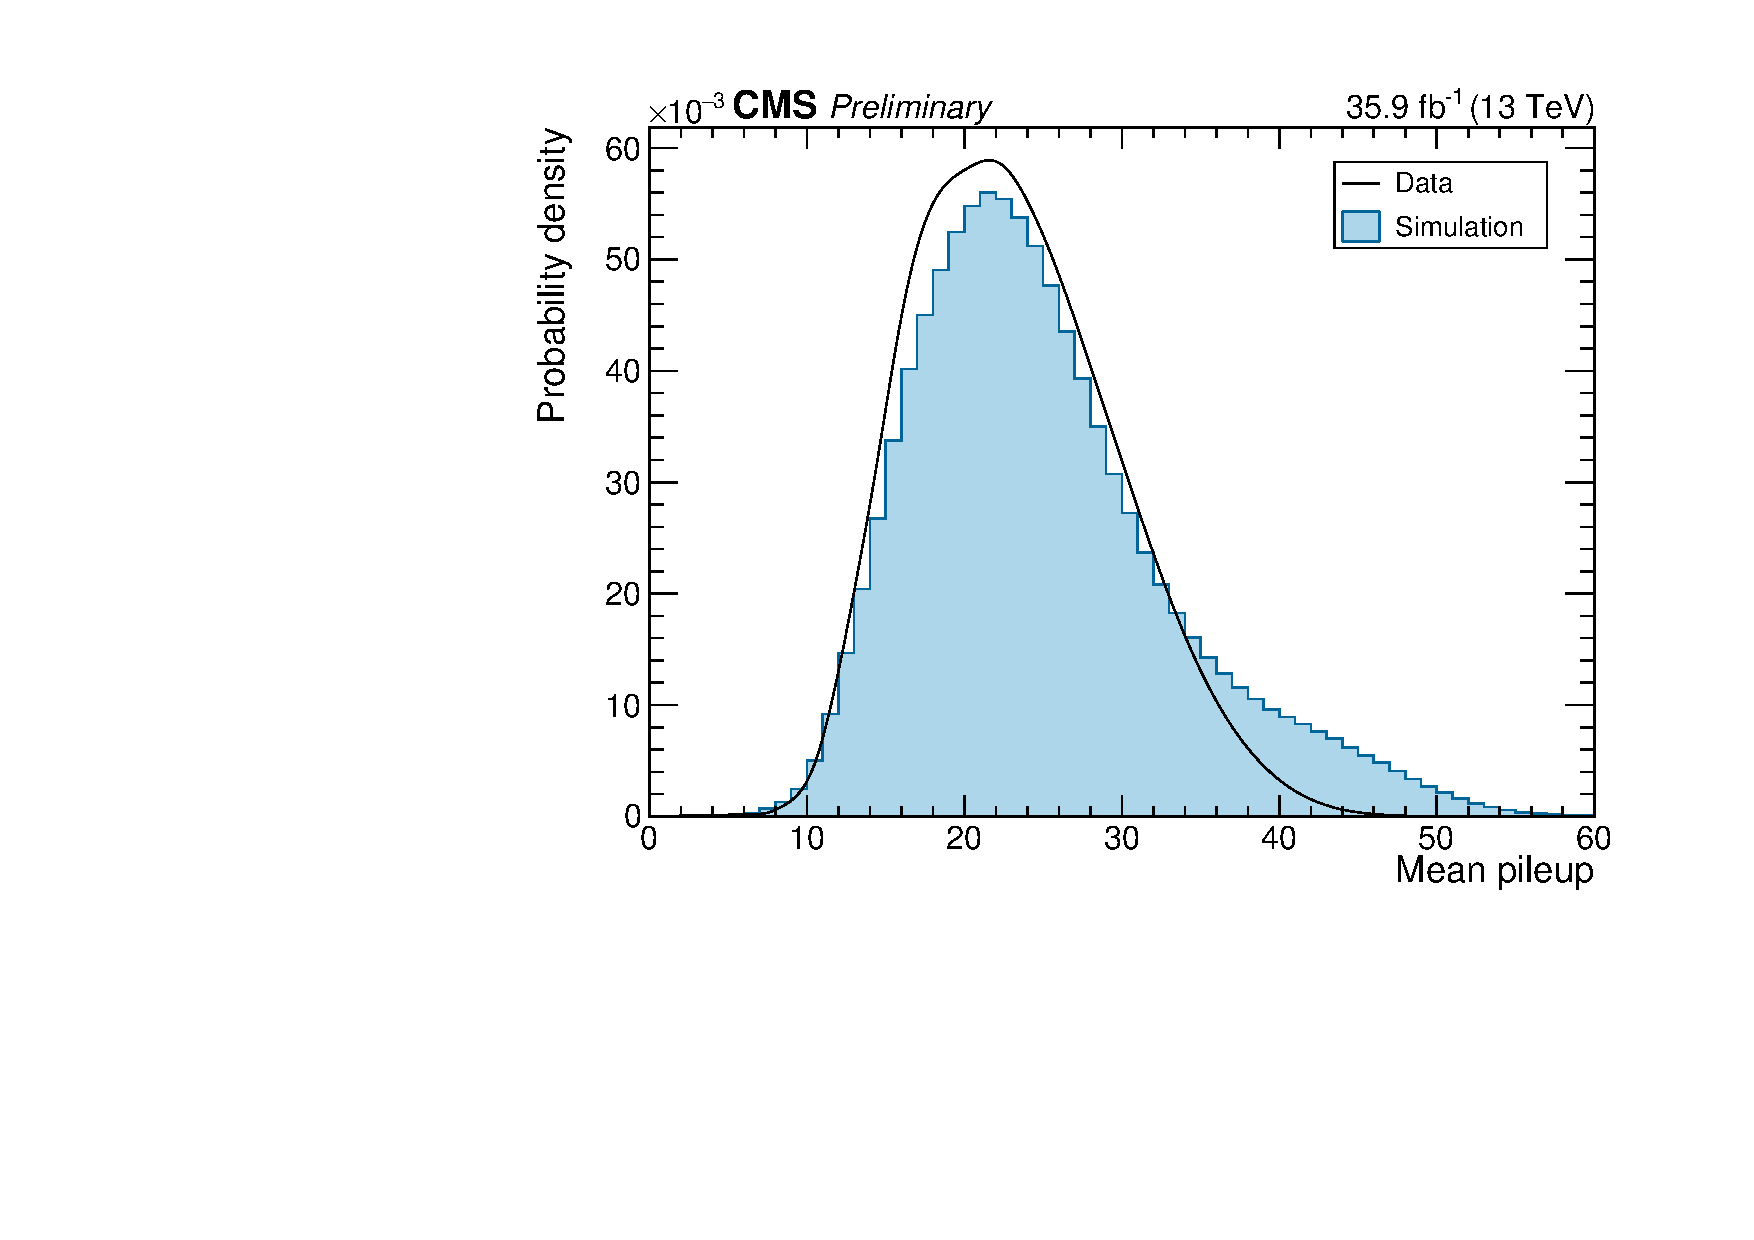
\includegraphics[width=0.6\textwidth]{fig/chapt7/correction/pileup-profiles.pdf}
  \caption{Pile-up profiles in data and simulation without corrections.}
  \label{Fig:PUProfiles}
\end{figure}


\subsection{Jet Energy Scale and Resolution}\label{sec:jes_jer}
Jet Energy Corrections (JEC) are applied to calibrate jets in order to have the correct energy scale like other experimental objects.
Jet energy scale corrections are applied to the reconstructed jets in simulation using the so called \texttt{Summer16\_23Sep2016ReReco\_V4}~\cite{wiki:jec} to have the correct energy scale as observed in data.\\
Jet Energy Resolution (JER) gives the spread of the response in the Gaussian core region and is different from JEC. In simulation the nominal jet energy resolution is smeared using a $p_{T}, \eta$-dependent parameterization~\cite{wiki:jer}. This analysis uses the recommended ``hybrid'' method for JER.


\subsection{B tagging}
\label{Sec:BTagReweighting}
%
The identification of b-jet is very important for the study of top quark decays, Higgs decay and many new physics phenomena. b-tagging is a reconstruction technique that takes advantage of the b hadron properties and assigns to each jet a likelihood that contains a b hadron. Following are the b-jets characteristics which discriminate them from jets produced by light quarks and gluons.
\begin{itemize}
\item Long life time: $\tau \sim$ 1.5 ps, $c\tau \sim$ 450 $\mu $m
\item Large mass: mass $\sim$ 4.2 GeV 
\item High track multiplicity $\sim$ 4-5
\item Large semileptonic branching fraction 
\end{itemize}
We use the combined multivariate algorithm (cMVAv2) that combines information from six different b-jet identification discriminators with a Boosted Decision Tree (BDT)~\cite{cms_pas_cmvav2}. cMVAv2 has three operating points, loose, medium and tight and this analysis uses the medium working point with cMVAv2 > 0.4432. 
Performance of b-tagging algorithms in data is known to be slightly worse than expected from simulation~\cite{CMS-PAS-BTV-15-001}.
In order to account for the difference, the b-tagging efficiencies in simulation are modified with the help of scale factors provided by the BTV POG~\cite{Wiki:BTagSF}.
There are several ways to perform the correction.
This search utilizes method~1a from Ref.~\cite{Wiki:BTagSFMethods}, which is summarized below.

For each simulated event the probability to reproduce the observed b-tagging configuration is given by
\begin{linenomath}
\begin{equation}
\mathcal P_\text{Sim} = \prod_{i\in\text{tagged}} \epsilon_i \enspace \cdot \prod_{j\notin\text{tagged}} (1 - \epsilon_j),
\end{equation}
\end{linenomath}
where $\epsilon_i$ is the b-tagging efficiency for jet~$i$ in simulation, and the first (second) product is calculated over b-tagged (not b-tagged) jets.
The probability to reproduce the same b-tagging configuration with efficiencies as in data reads as
\begin{linenomath}
\begin{equation}
\mathcal P_\text{Data} = \prod_{i\in\text{tagged}} s_i\epsilon_i \enspace \cdot \prod_{j\notin\text{tagged}} (1 - s_j\epsilon_j),
\end{equation}
\end{linenomath}
where $s_i$ is the scale factor for jet~$i$, which is parameterized as a function of $p_{T}$, $\eta$, and flavour of the jet.
In this analysis scale factors from the payload ``\texttt{ttbar}'' (``\texttt{incl}'') are used for b and c~quark (light-flavour) jets.
To account for the mismodelling of the b-tagging probabilities, the event is assigned a weight
\begin{linenomath}
\begin{equation}
\label{Eq:WeightBTag}
w = \mathcal P_\text{Data} / \mathcal P_\text{Sim} = \prod_{i\in\text{tagged}} s_i \enspace \cdot \prod_{j\notin\text{tagged}} \frac{1 - s_j\epsilon_j}{1 - \epsilon_j}.
\end{equation}
\end{linenomath}

The b-tagging efficiencies in simulation, which are needed to determine the weight, depend on the physics process and the event selection and therefore cannot be provided centrally.
They have been computed after applying the full analysis event selection (which will be described later) but b-tagging.
The measurement is done with only the $t\bar t$ sample as this is by far the dominant background and also representative of jet properties in the signal process.
The efficiencies are parameterized with jet $p_{T}$, $\eta$, and flavour, with the three usual flavour categories considered: b and c~quark jets and all the rest.

The effect of b-tagging correction is shown on leading b-jet $p_{T}$ in Fig.~\ref{fig:btag_correction}, (a) is without b-tagging correction while correction is applied in (b). 
\begin{figure}[htp]
\centering
\begin{tabular}{cc}
\hspace{-0.5cm}
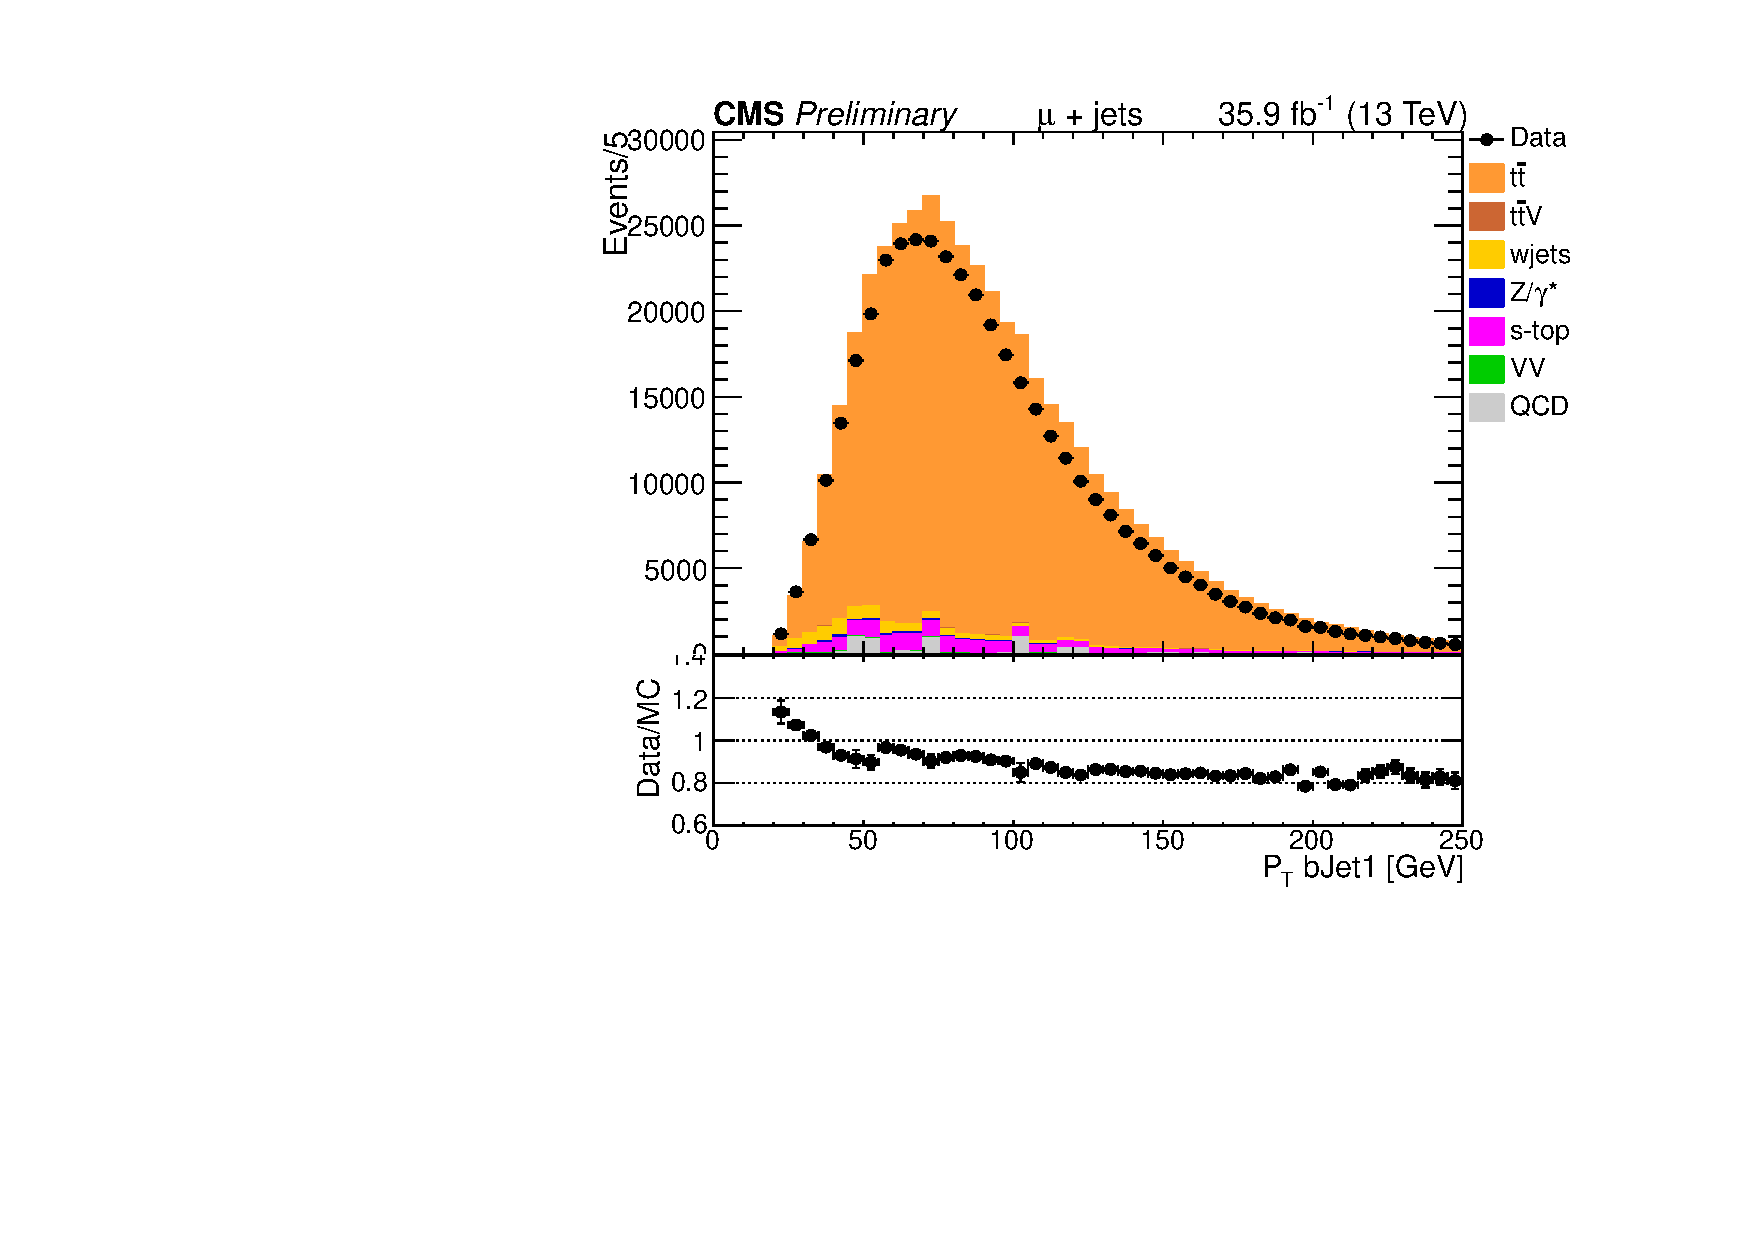
\includegraphics[scale=0.45]{fig/chapt7/correction/btag_nocorrection_Pt_bJet1.pdf}
& \hspace{-1.50cm} 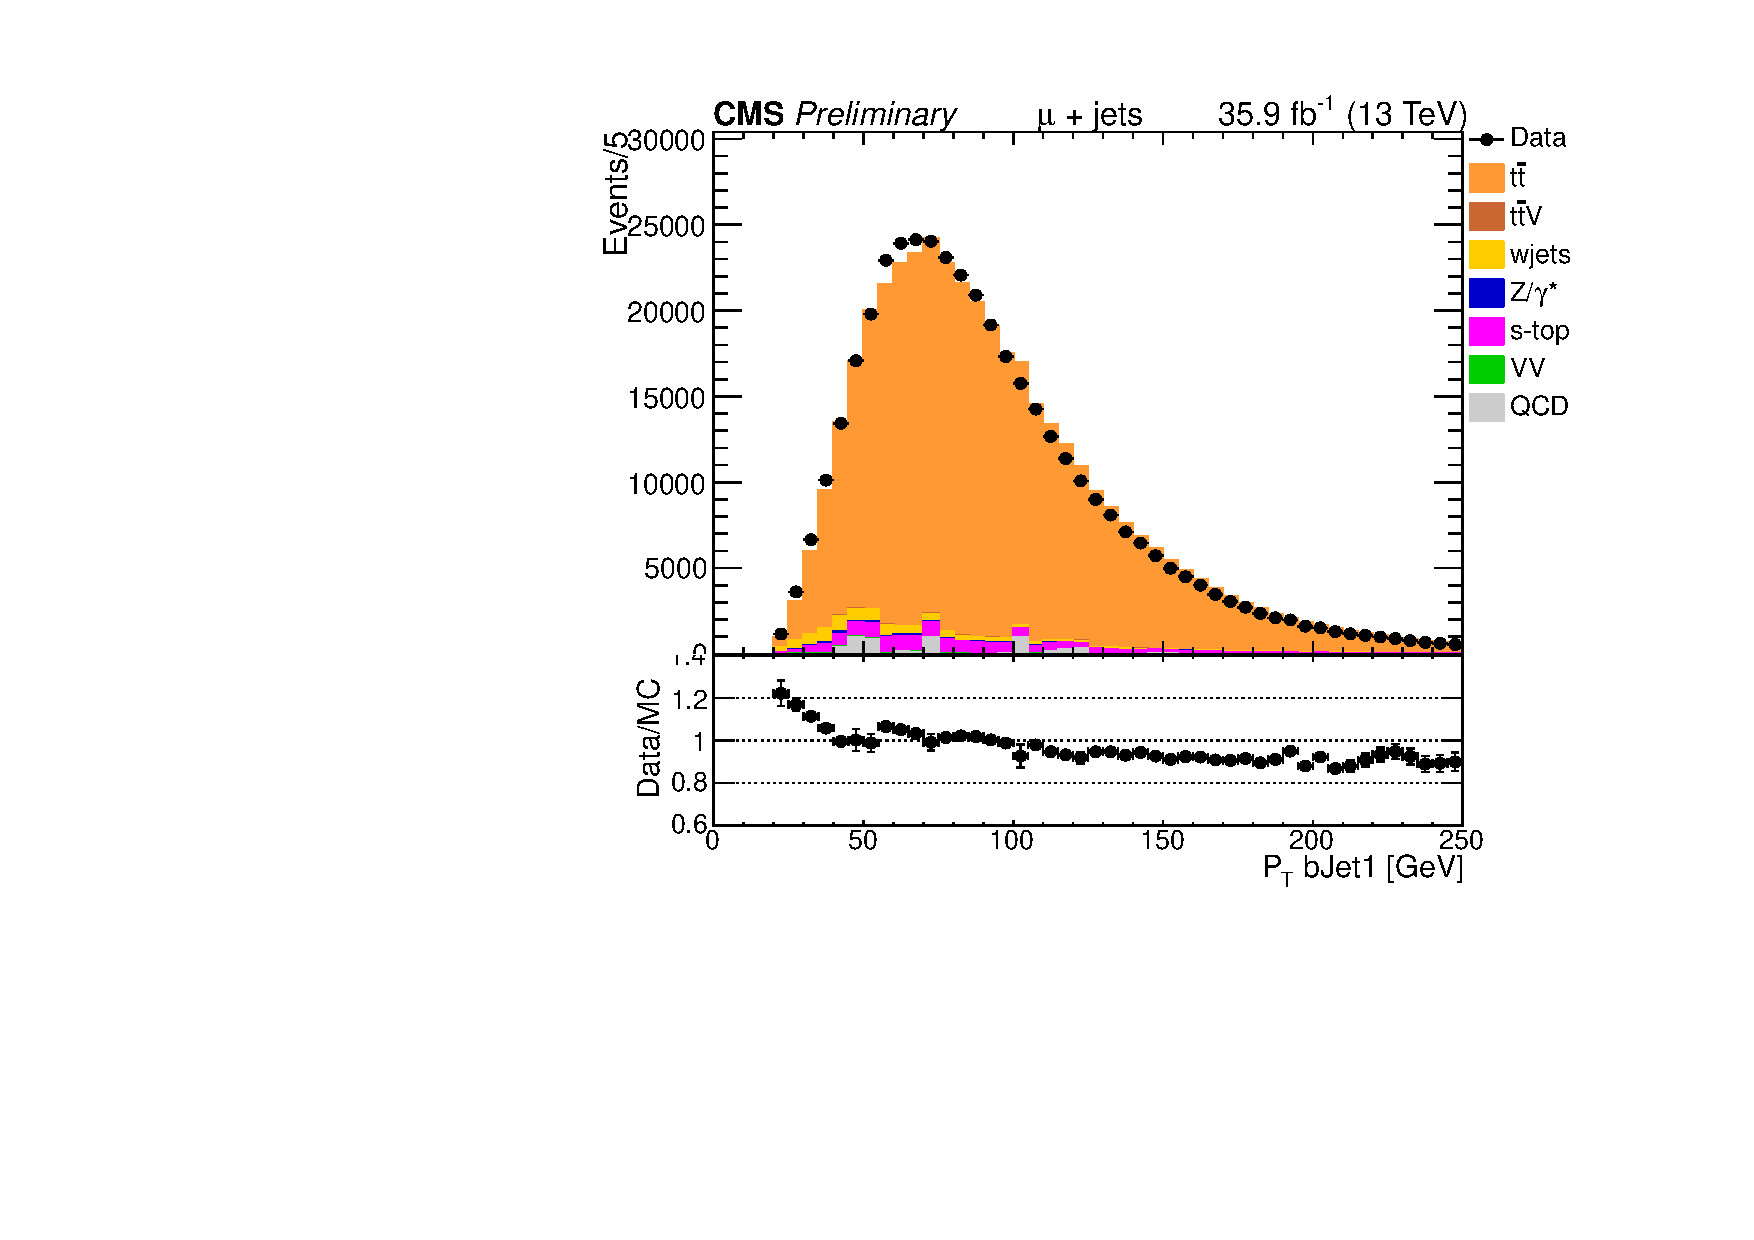
\includegraphics[scale=0.45]{fig/chapt7/correction/btag_correction_Pt_bJet1.pdf}\\
  \qquad ($\mathbf{a}$)\qquad\qquad&($\mathbf{b}$)\qquad\qquad\qquad\qquad \\
\end{tabular}
\caption{Transverse momentum of first b-tagged jet in data and MC pre (a) and post (b) b-tagging correction in the $t\bar{t}$ dominated region using muon channel. Data/MC comparison improves after applying jet energy correction.}\label{fig:btag_correction}
\end{figure}

%\subsection{Efficiency of trigger \texorpdfstring{\texttt{HLT\char`_Ele27\char`_WPTight\char`_Gsf}}{HLT\_Ele27\_WPTight\_Gsf}}\label{subsec:elec_trigg}
\subsection{Trigger efficiency}\label{subsec:elec_trigg}
%
\textbf{Electron trigger efficiency}: Corrections to efficiency of electron trigger \texttt{HLT\char`_Ele27\char`_WPTight\char`_Gsf\char`_v*}, which is used in this search, are not provided centrally.
Instead, a dedicated measurement is performed in a sample of $Z \rightarrow e^+e^-$ events using the tag-and-probe method~\cite{CMS-AN-09-111, Khachatryan:2010xn, CMS-AN-12-116}.
Results discussed below have been presented before EGM~POG and approved~\cite{Talk:EleTriggerSF}.

The method exploits two sets of selections for electrons.
A ``tag'' electron is required to have $p_{T} > 40$~GeV{} and $|\eta_\text{SC}| < 2.1$, not fall in the transition region between the barrel and the endcaps of the ECAL ($1.4442 < |\eta_\text{SC}| < 1.5660$), and pass the tight working point of the cut-based identification algorithm and the recommended additional selection on impact parameters.
It must also be matched, within $\Delta R < 0.3$, to a trigger object passing the last filter in trigger \texttt{HLT\char`_Ele27\char`_WPTight\char`_Gsf\char`_v*}.
Finally, it is required to be matched, also within $\Delta R < 0.3$, to an L1T $e/\gamma$ object that passes trigger \texttt{L1\char`_SingleIsoEG34er}.
This last condition is needed because all single-electron HLT paths in 2016 are seeded by an inclusive~\textit{or} of all available single-$e/\gamma$ L1T~seeds, most of which were prescaled during some periods of data taking.
The lowest-$p_{T}$ seed that was never prescaled is \texttt{L1\char`_SingleIsoEG34er} (although \texttt{L1\char`_SingleIsoEG32er} was unprescaled in the full data set but few pb$^{-1}$).
The matching to the L1T~seed guarantees that the sample of selected events is not biased in terms of prescales of L1T~seeds with lower thresholds~\cite{Talk:L1EGPrescales}.
The other set of requirements defines a ``probe'' electron.
It is subject to a looser selection, requiring $p_{T} > 25$~GeV and $|\eta_\text{SC}| < 2.5$ and asking for the tight working point of the identification algorithm and the additional selection on impact parameters.
If a ``probe'' is additionally matched to one of the considered HLT objects, it is referred to as a ``passing probe''.
Efficiency of the trigger under study is determined as the probability for a ``probe'' electron to be also a ``passing probe''.
It is parameterized with the transverse momentum of the electron and the pseudorapidity of the associated ECAL supercluster, which allows to apply the measurement to electrons used in this search despite the fact that they are defined with a tighter selection on~$p_{T}$ and with the transition region between the barrel and the endcaps excluded.

Trigger efficiency is measured in data as well as in simulation of the Drell-Yan process using events selected by trigger \texttt{HLT\char`_Ele27\char`_WPTight\char`_Gsf\char`_v*} and containing exactly two ``probe'' electrons with opposite electric charges, at least one of which also satisfies definition of a ``tag''.
Invariant mass of the pair of electrons must satisfy $60 < m_{e^+e^-} < 120$~GeV.
The tag-and-probe method allows to account for the presence of background with non-prompt leptons by fitting the $m_{e^+e^-}$~spectrum, taking an advantage of the non-peaking distributions for the background.
The fit, however, is not required in this case because the selected region is already very pure in $Z \rightarrow e^+e^-$ events.
The trigger efficiency is computed simply as
\begin{linenomath}
\begin{equation}
 \epsilon = \frac{N_\text{P}}{N_\text{P} + N_\text{F}},
\end{equation}
\end{linenomath}
where $N_\text{P}$ ($N_\text{F}$) is the number of tag--probe pairs with a passing (failing) ``probe''.
It should be noted that if both ``probes'' in an event are also ``tags'', this single event gives two tag--probe pairs, in which the two electrons are swapped.
Example distributions of $m_{ee}$ are shown in Fig.~\ref{Fig:TnPExamples}.
\begin{figure}
  \centering
  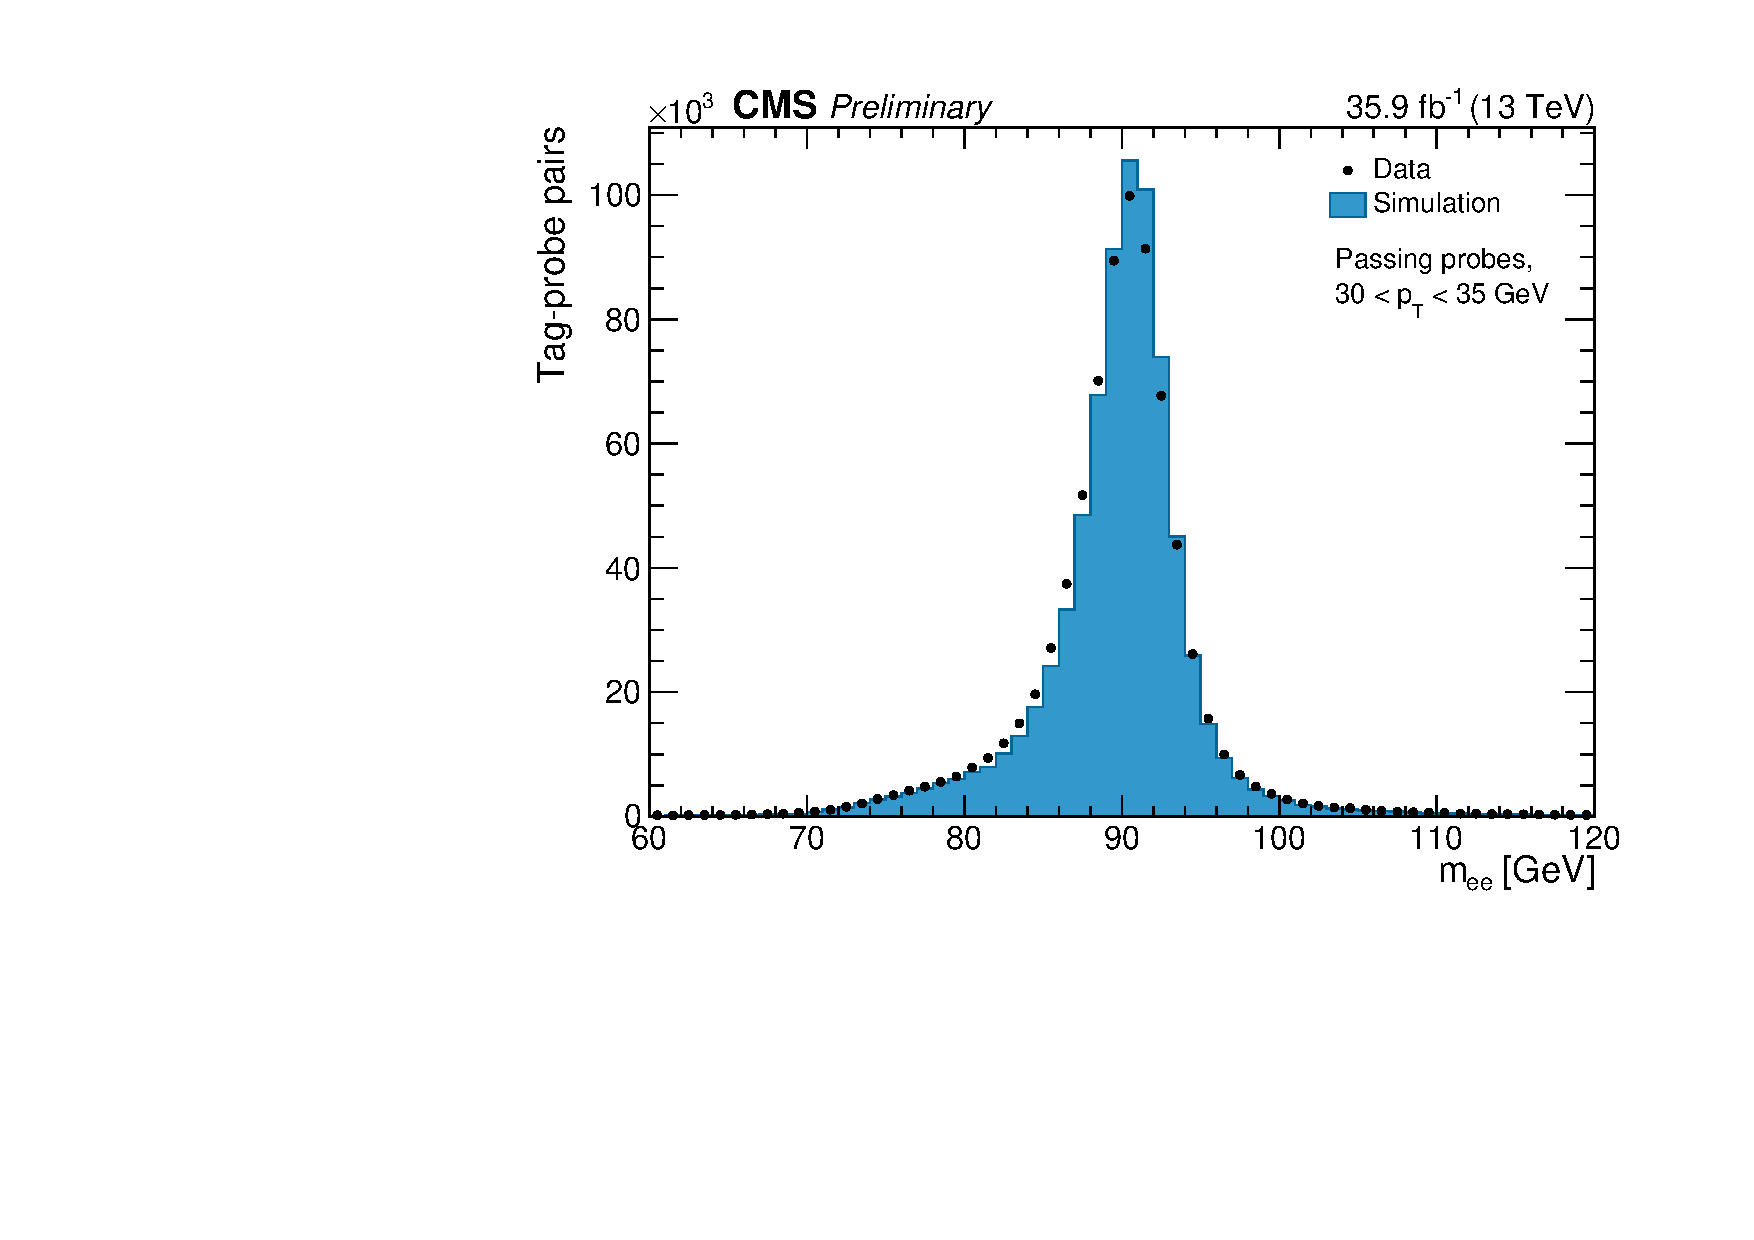
\includegraphics[width=0.45\textwidth]{fig/chapt7/trigger_eff/pass_pt30to35.pdf}
  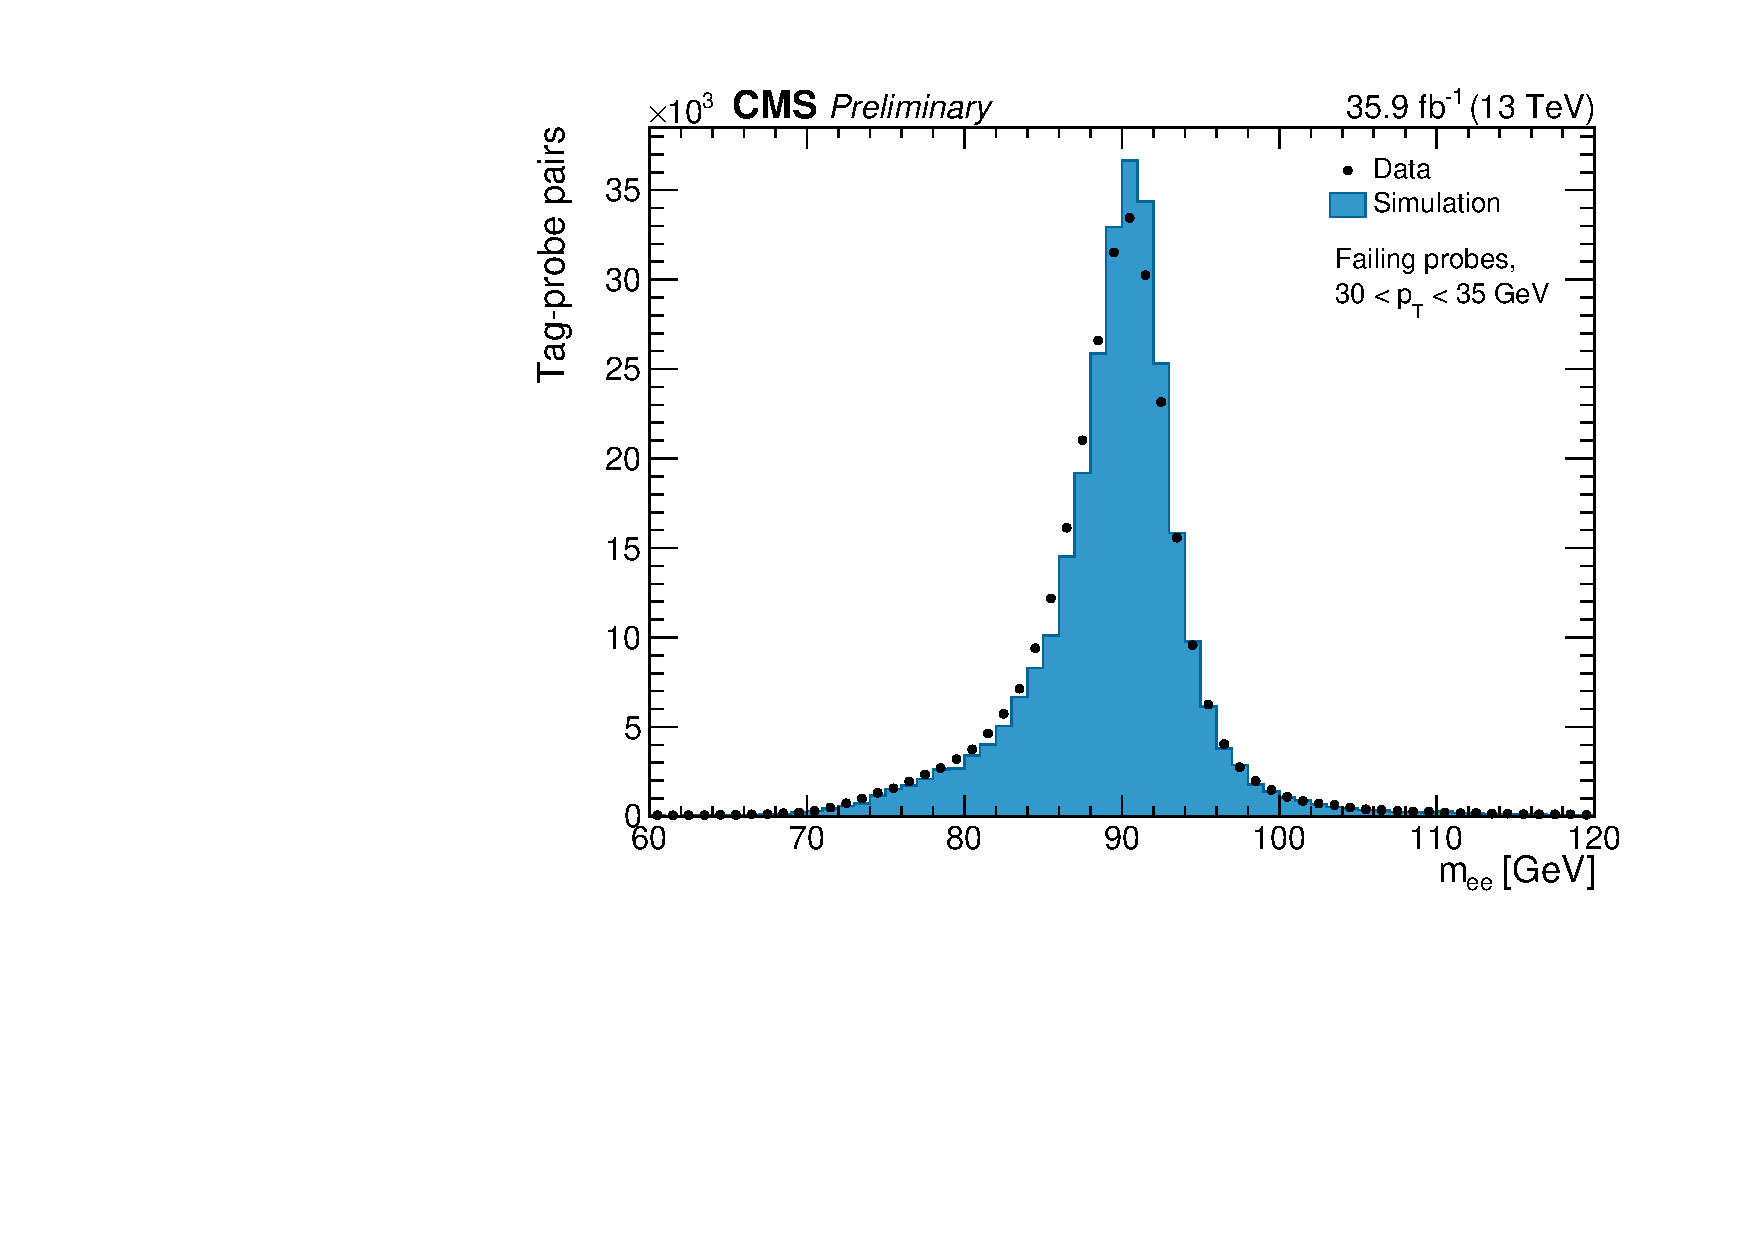
\includegraphics[width=0.45\textwidth]{fig/chapt7/trigger_eff/fail_pt30to35.pdf}
  \caption{Example distributions of $m_{ee}$ in tag--probe pairs with passing (left) and failing (right) ``probes''. Shown for $30 < p_{T}^\text{probe} < 35$~GeV.}
  \label{Fig:TnPExamples}
\end{figure}
Figure~\ref{Fig:TnP1DEff} shows one-dimensional trigger efficiencies as functions of different observables.
Compared to simulation, certain degradation of the efficiency is observed for low-$p_{T}$ electrons as well as in the forward region.
In part, this is an effect of imperfect transparency corrections for ECAL crystals.
A moderate dependence of the scale factors on the amount of pile-up is visible, which, however, will be absorbed in the final scale correction because simulation is reweighted to match the pile-up profile observed in data.
The dependence on the number of jets in the event will be covered by an additional uncertainty.

\begin{figure}
  \centering
  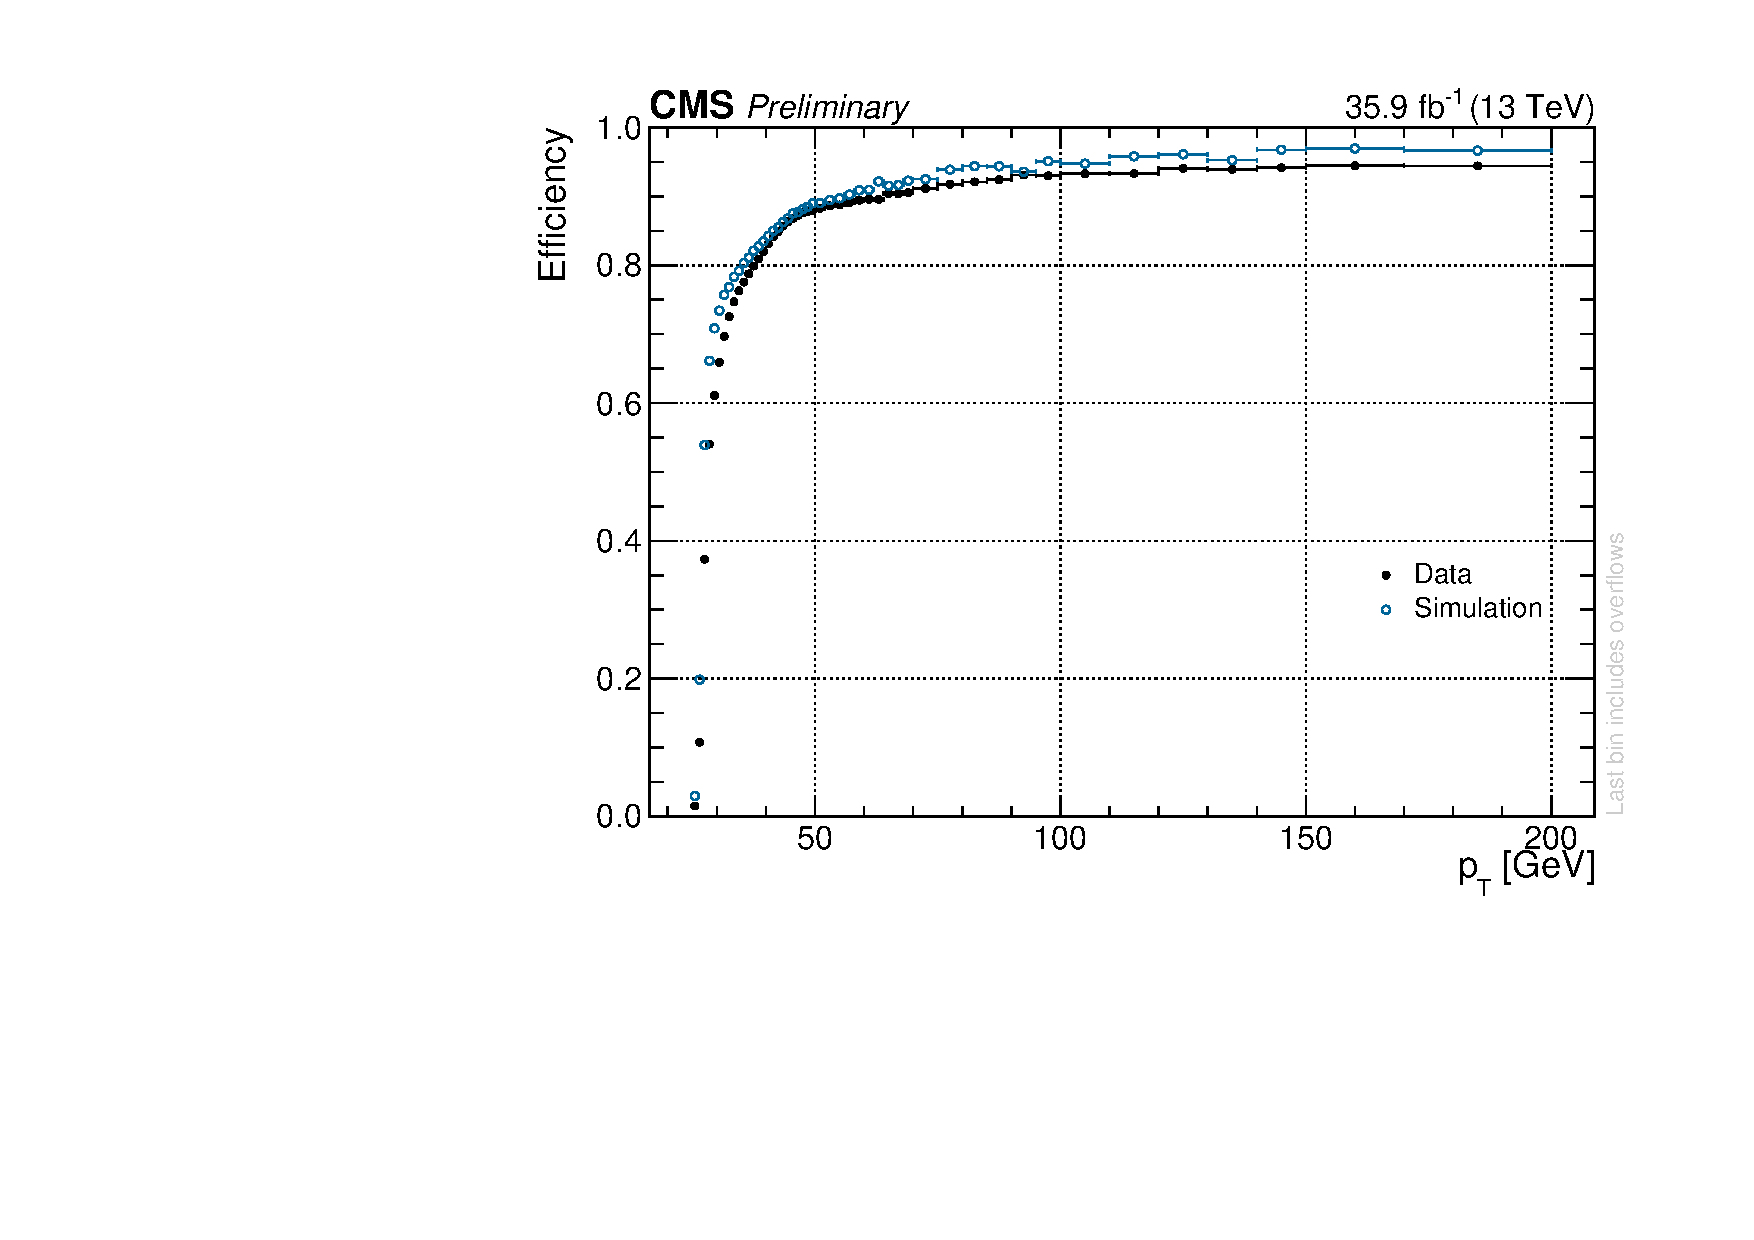
\includegraphics[width=0.45\textwidth]{fig/chapt7/trigger_eff/eff_pt.pdf}
  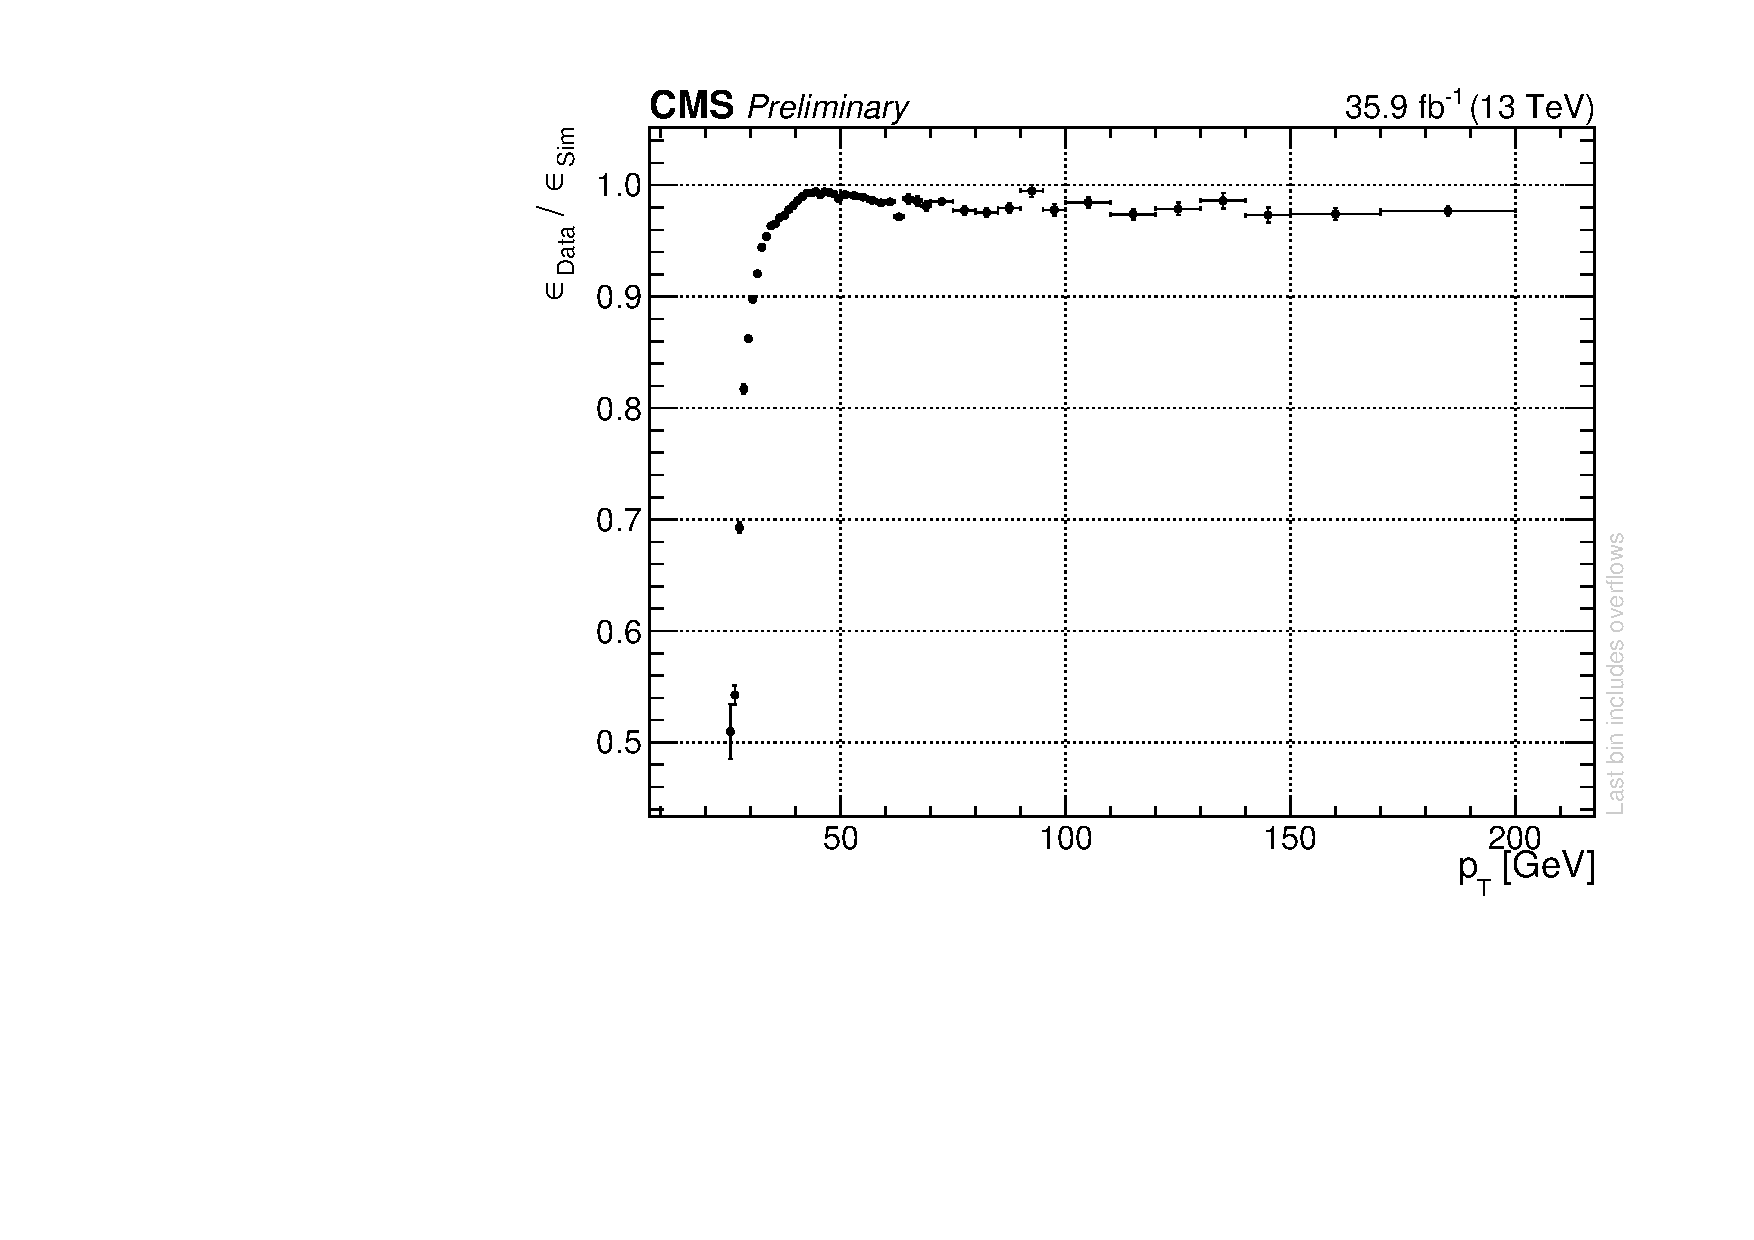
\includegraphics[width=0.45\textwidth]{fig/chapt7/trigger_eff/sf_pt.pdf} \\
  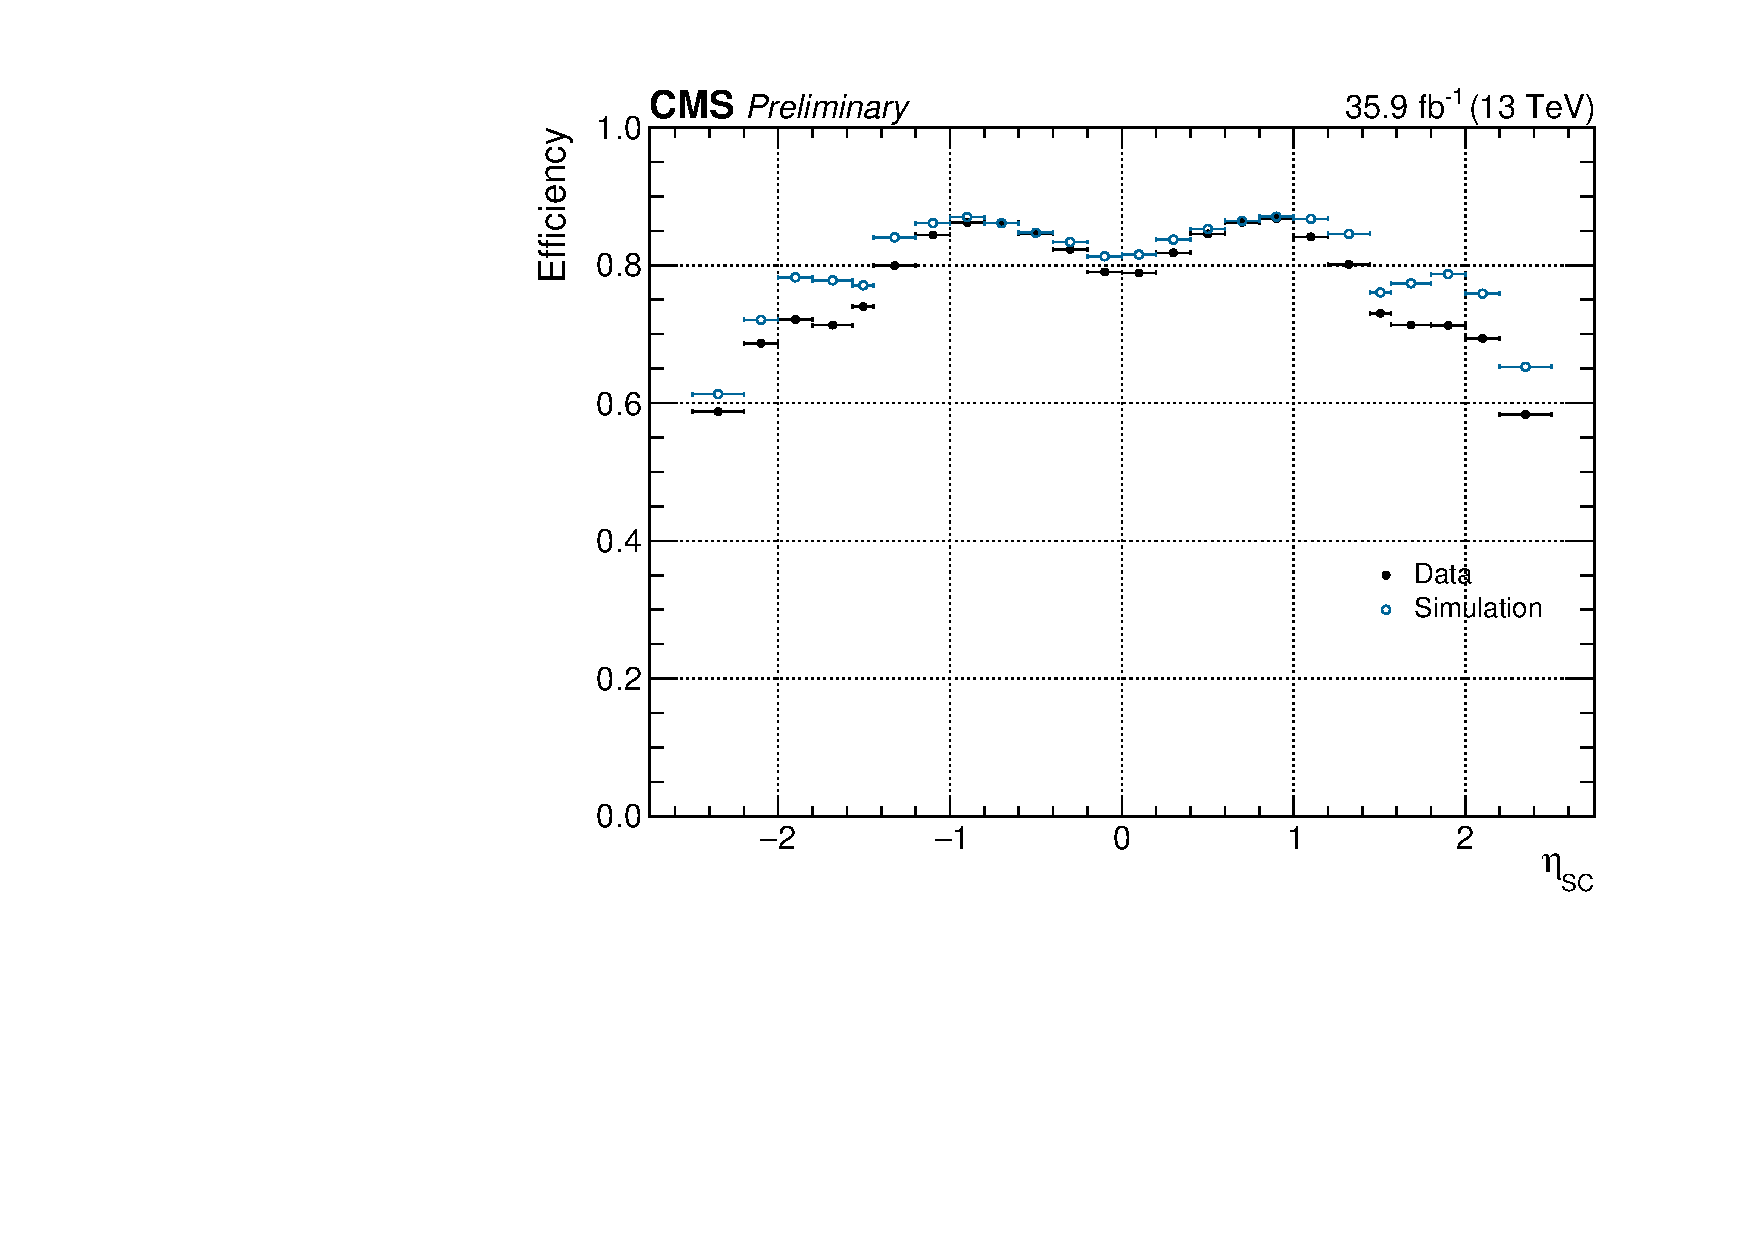
\includegraphics[width=0.45\textwidth]{fig/chapt7/trigger_eff/eff_eta.pdf}
  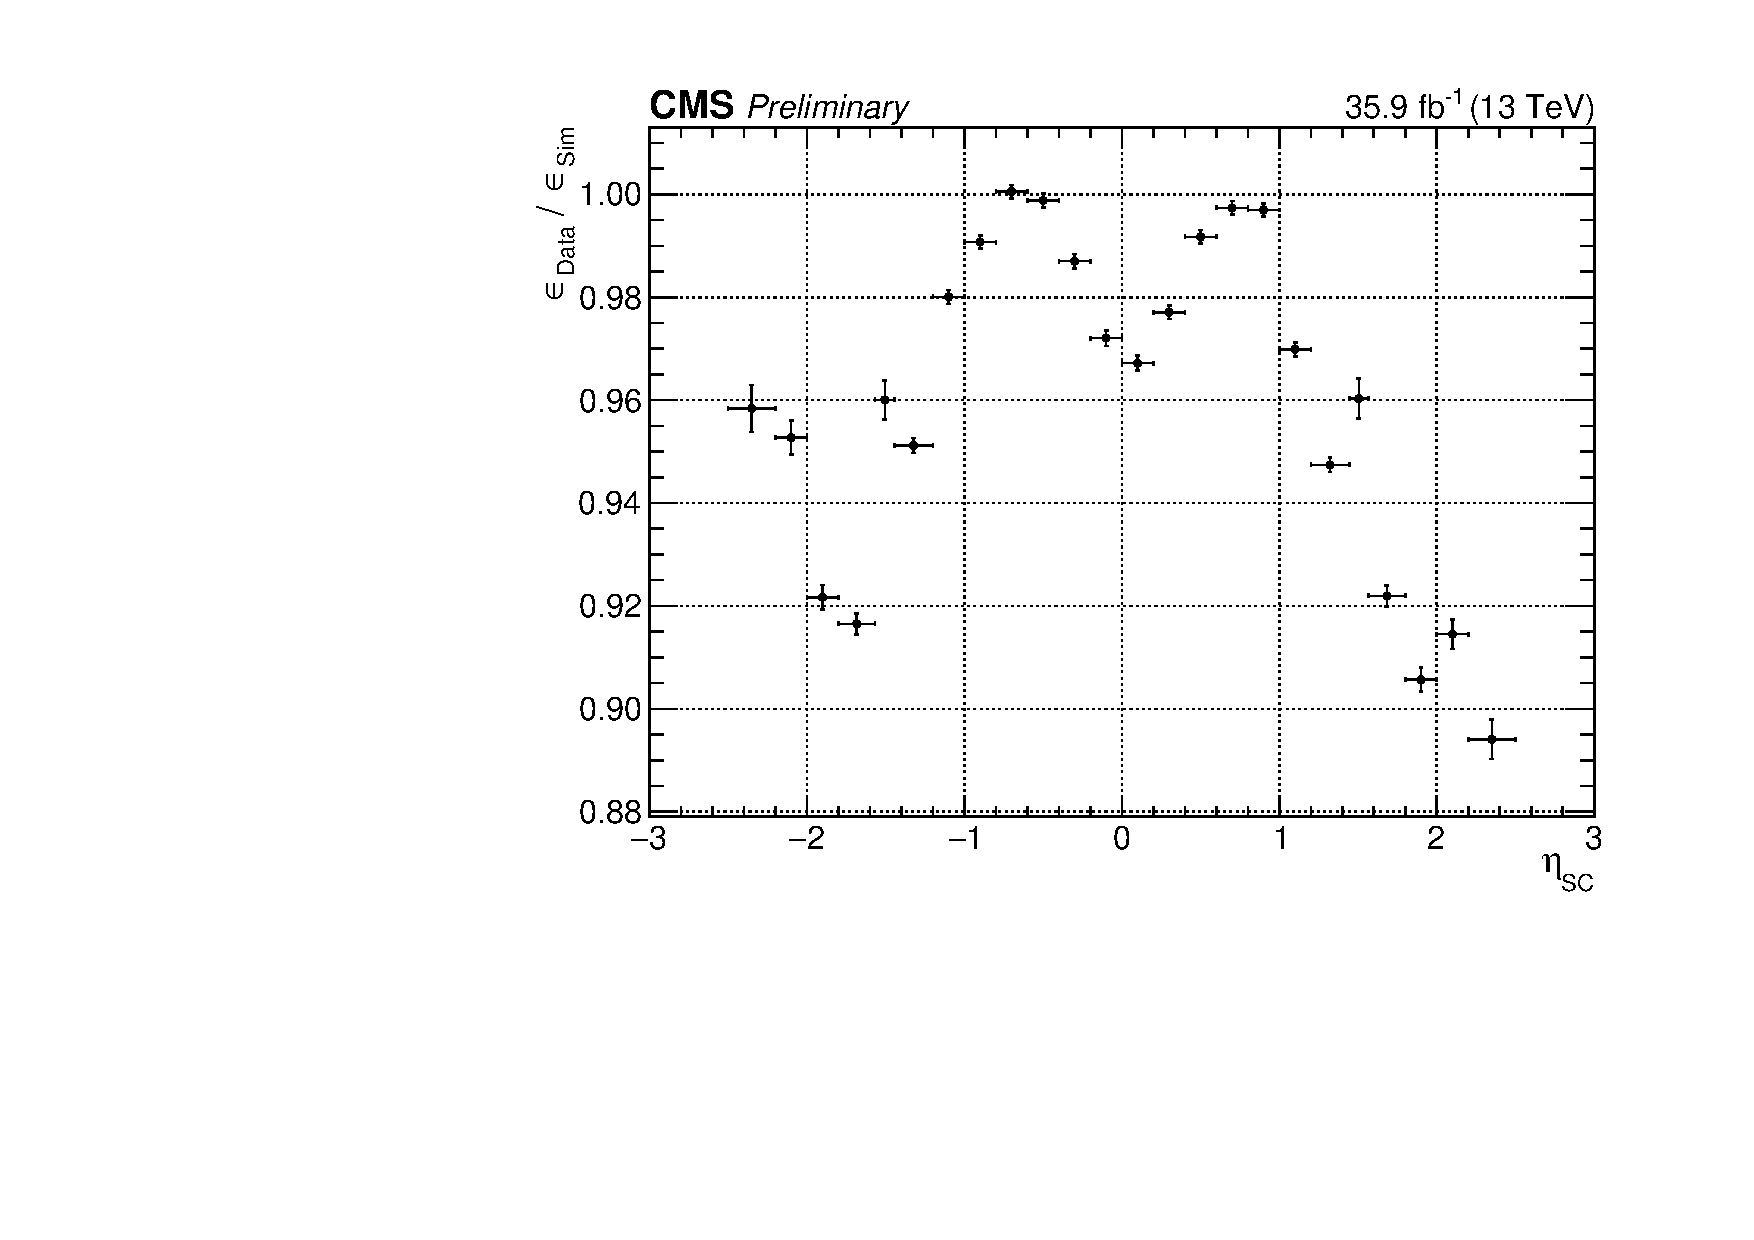
\includegraphics[width=0.45\textwidth]{fig/chapt7/trigger_eff/sf_eta.pdf} \\
  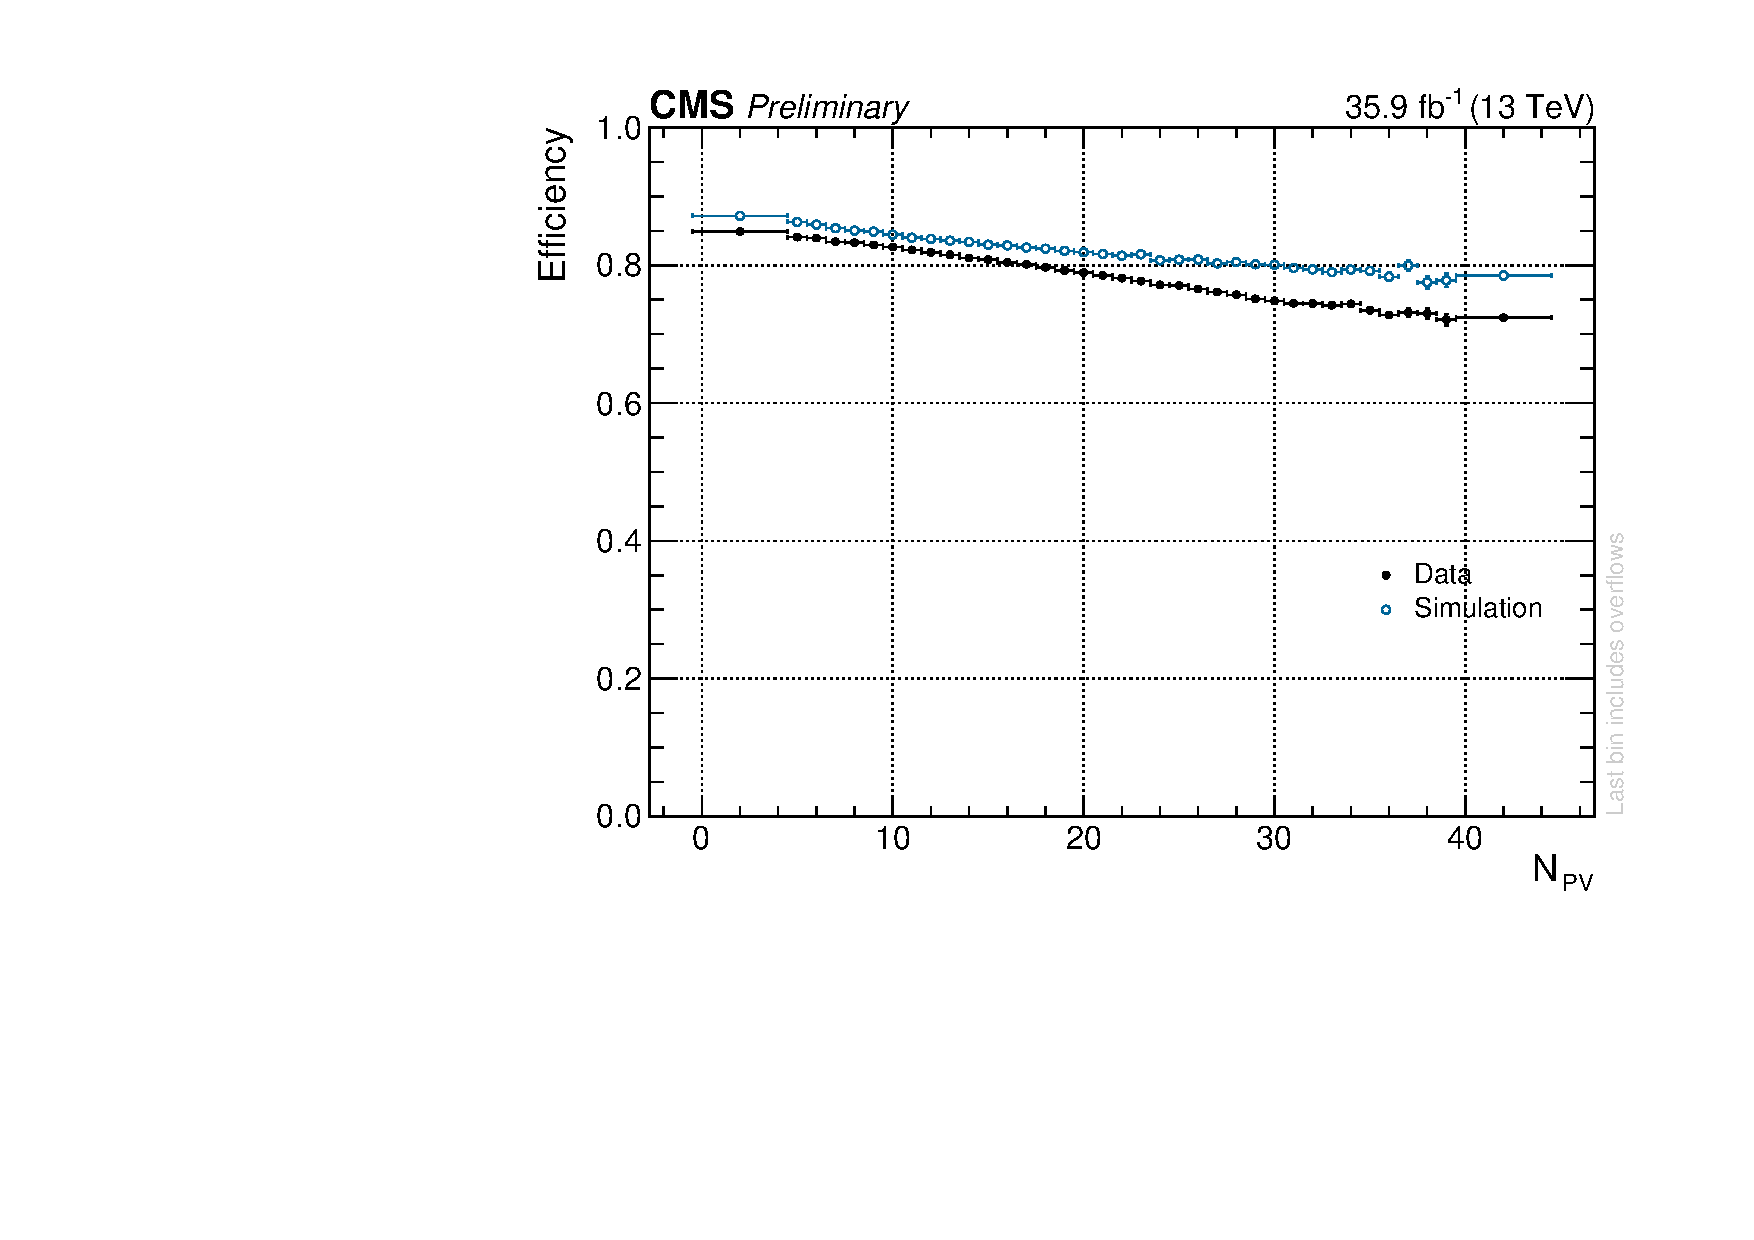
\includegraphics[width=0.45\textwidth]{fig/chapt7/trigger_eff/eff_PV.pdf}
  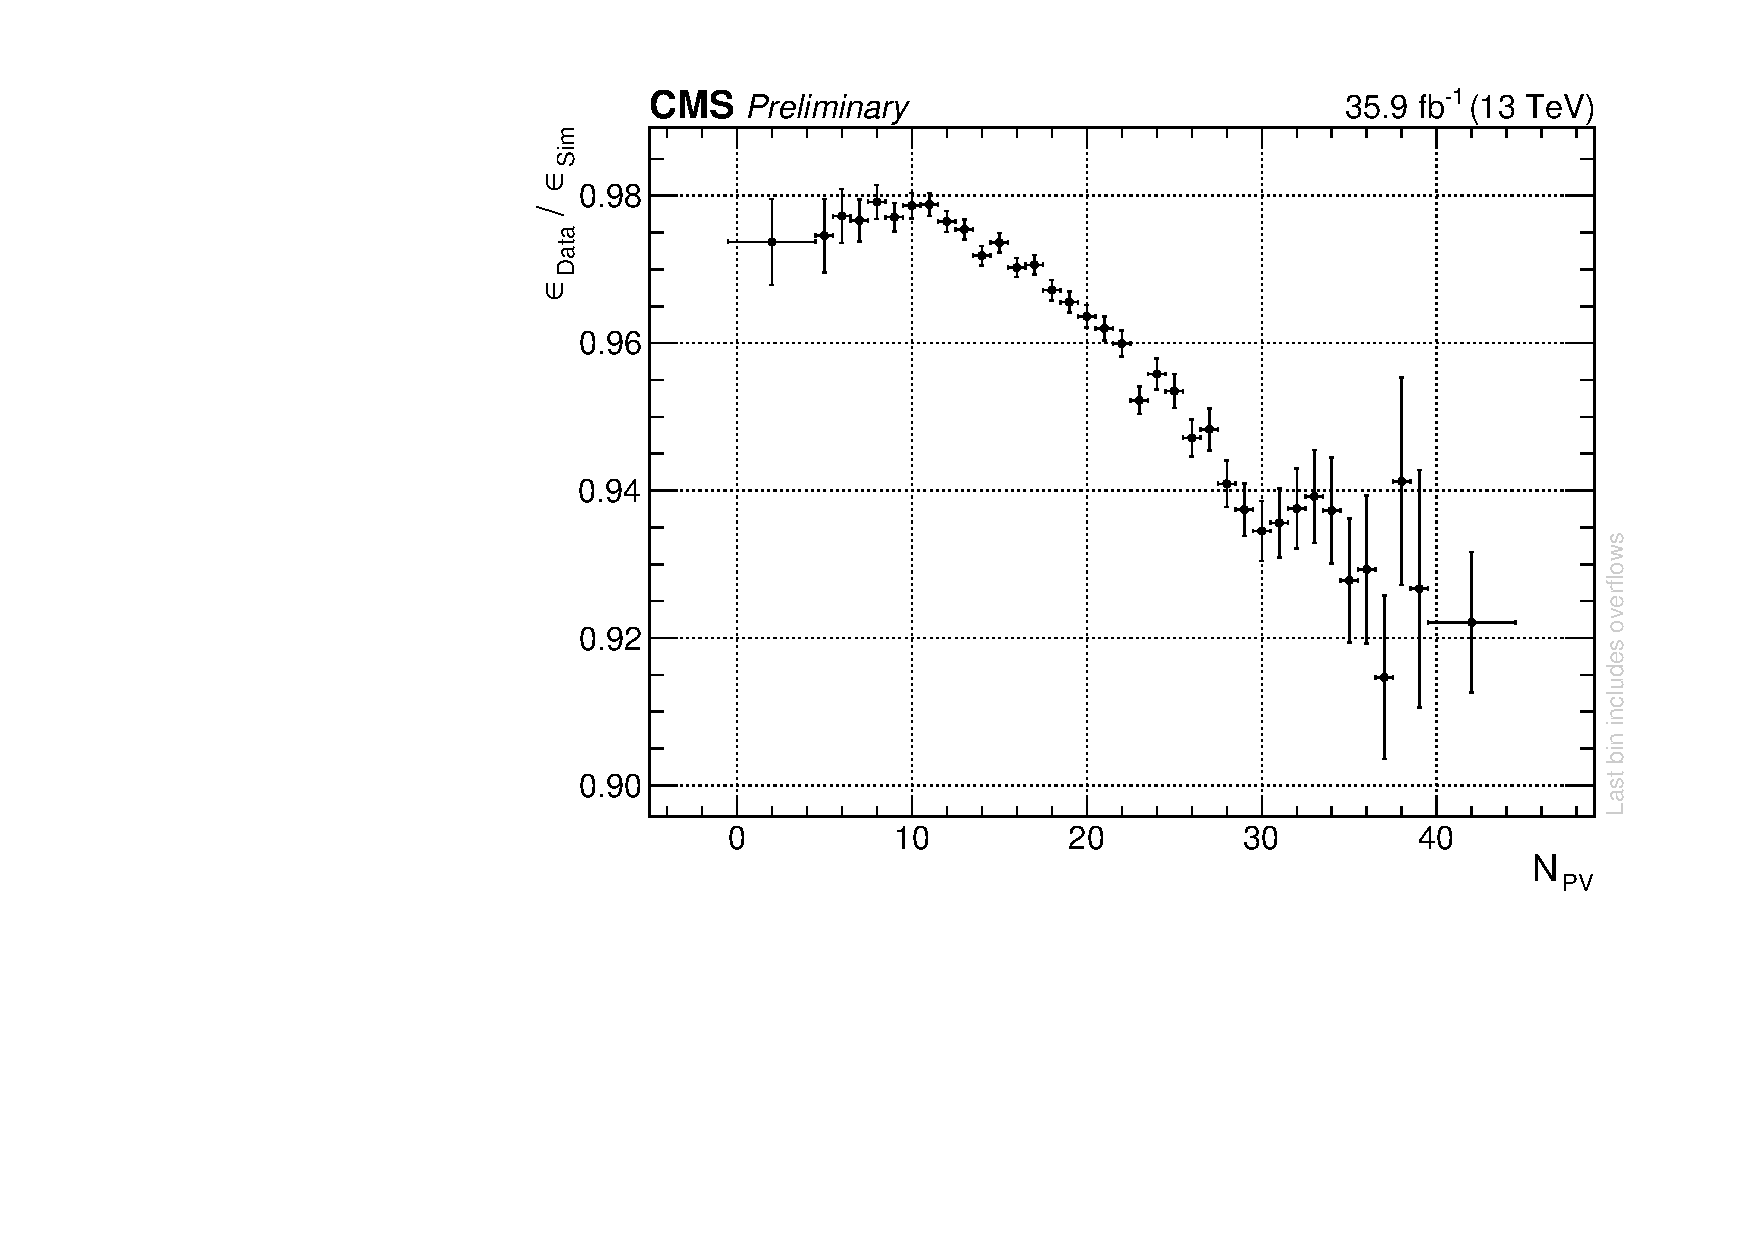
\includegraphics[width=0.45\textwidth]{fig/chapt7/trigger_eff/sf_PV.pdf} \\
  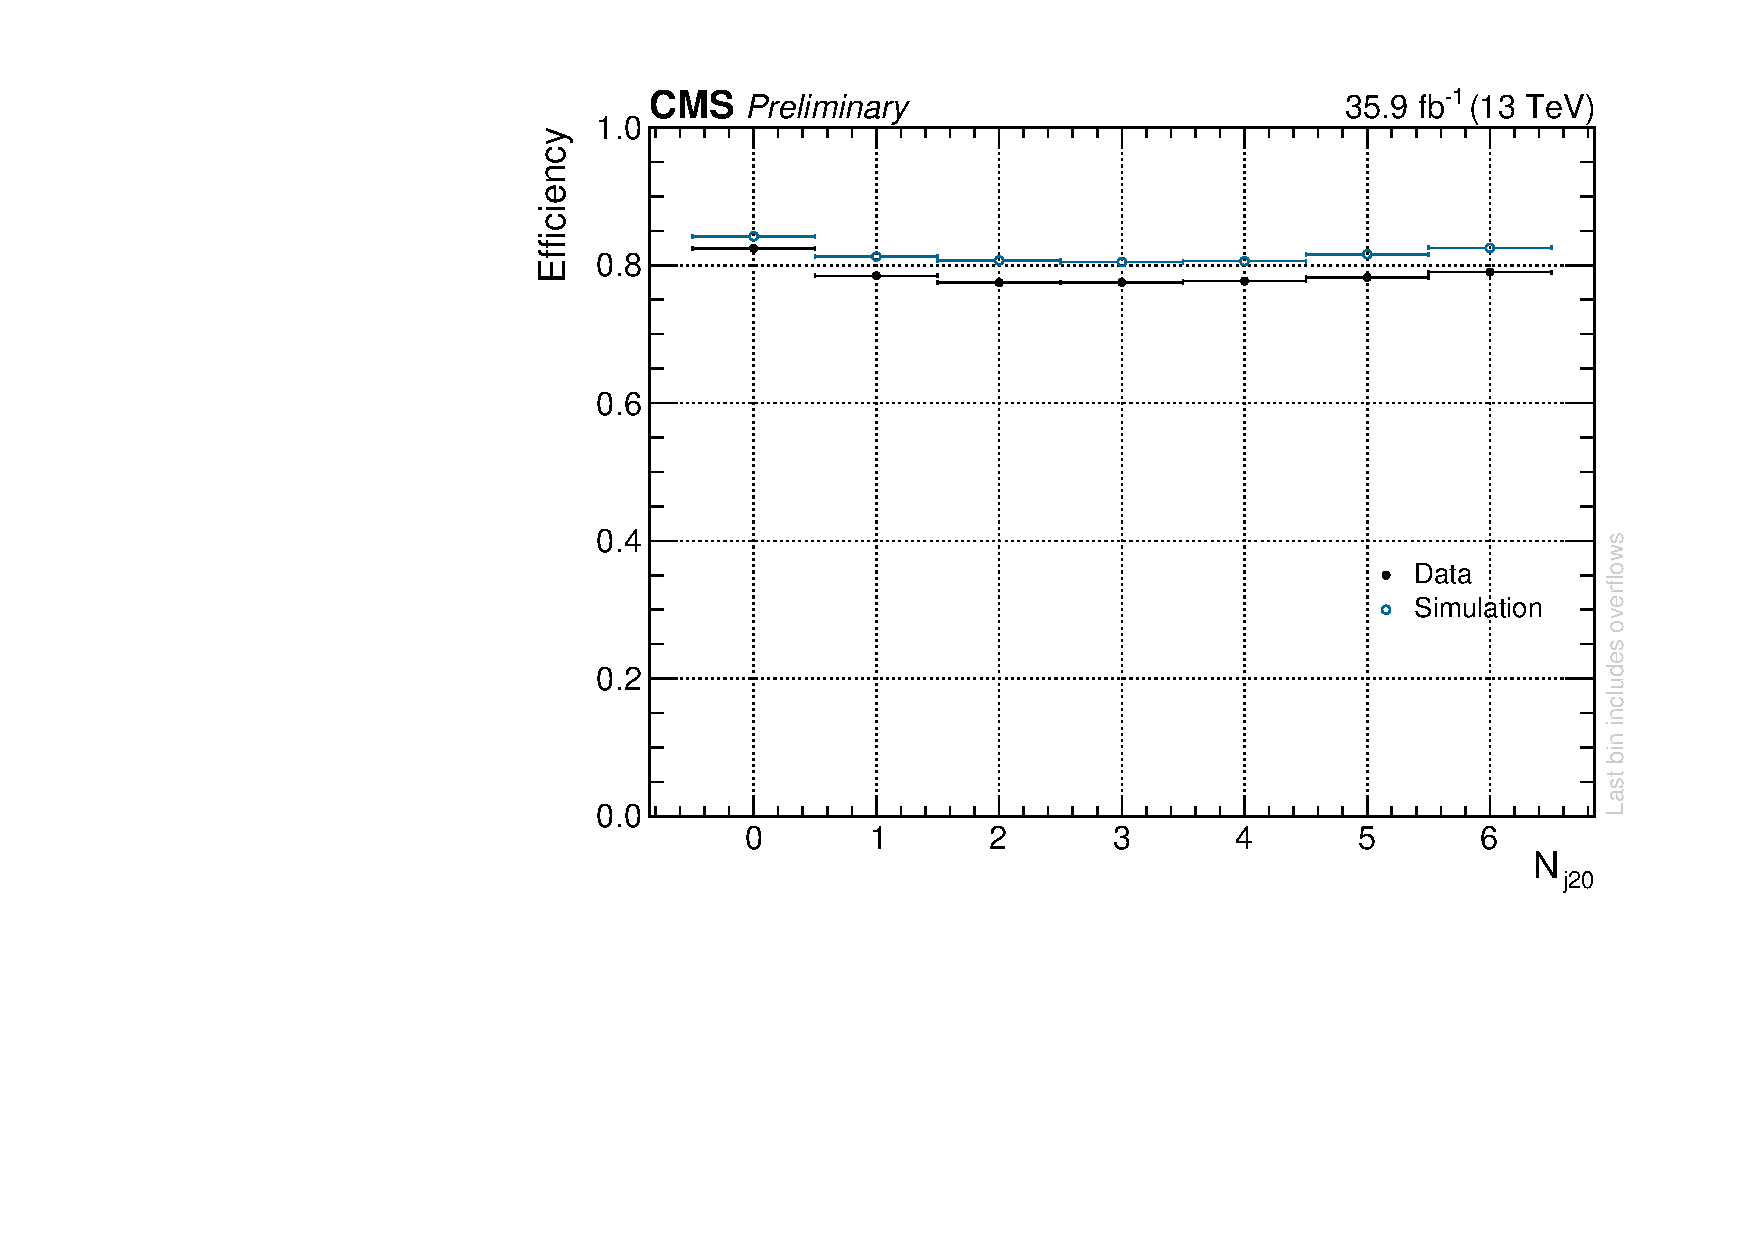
\includegraphics[width=0.45\textwidth]{fig/chapt7/trigger_eff/eff_jets.pdf}
  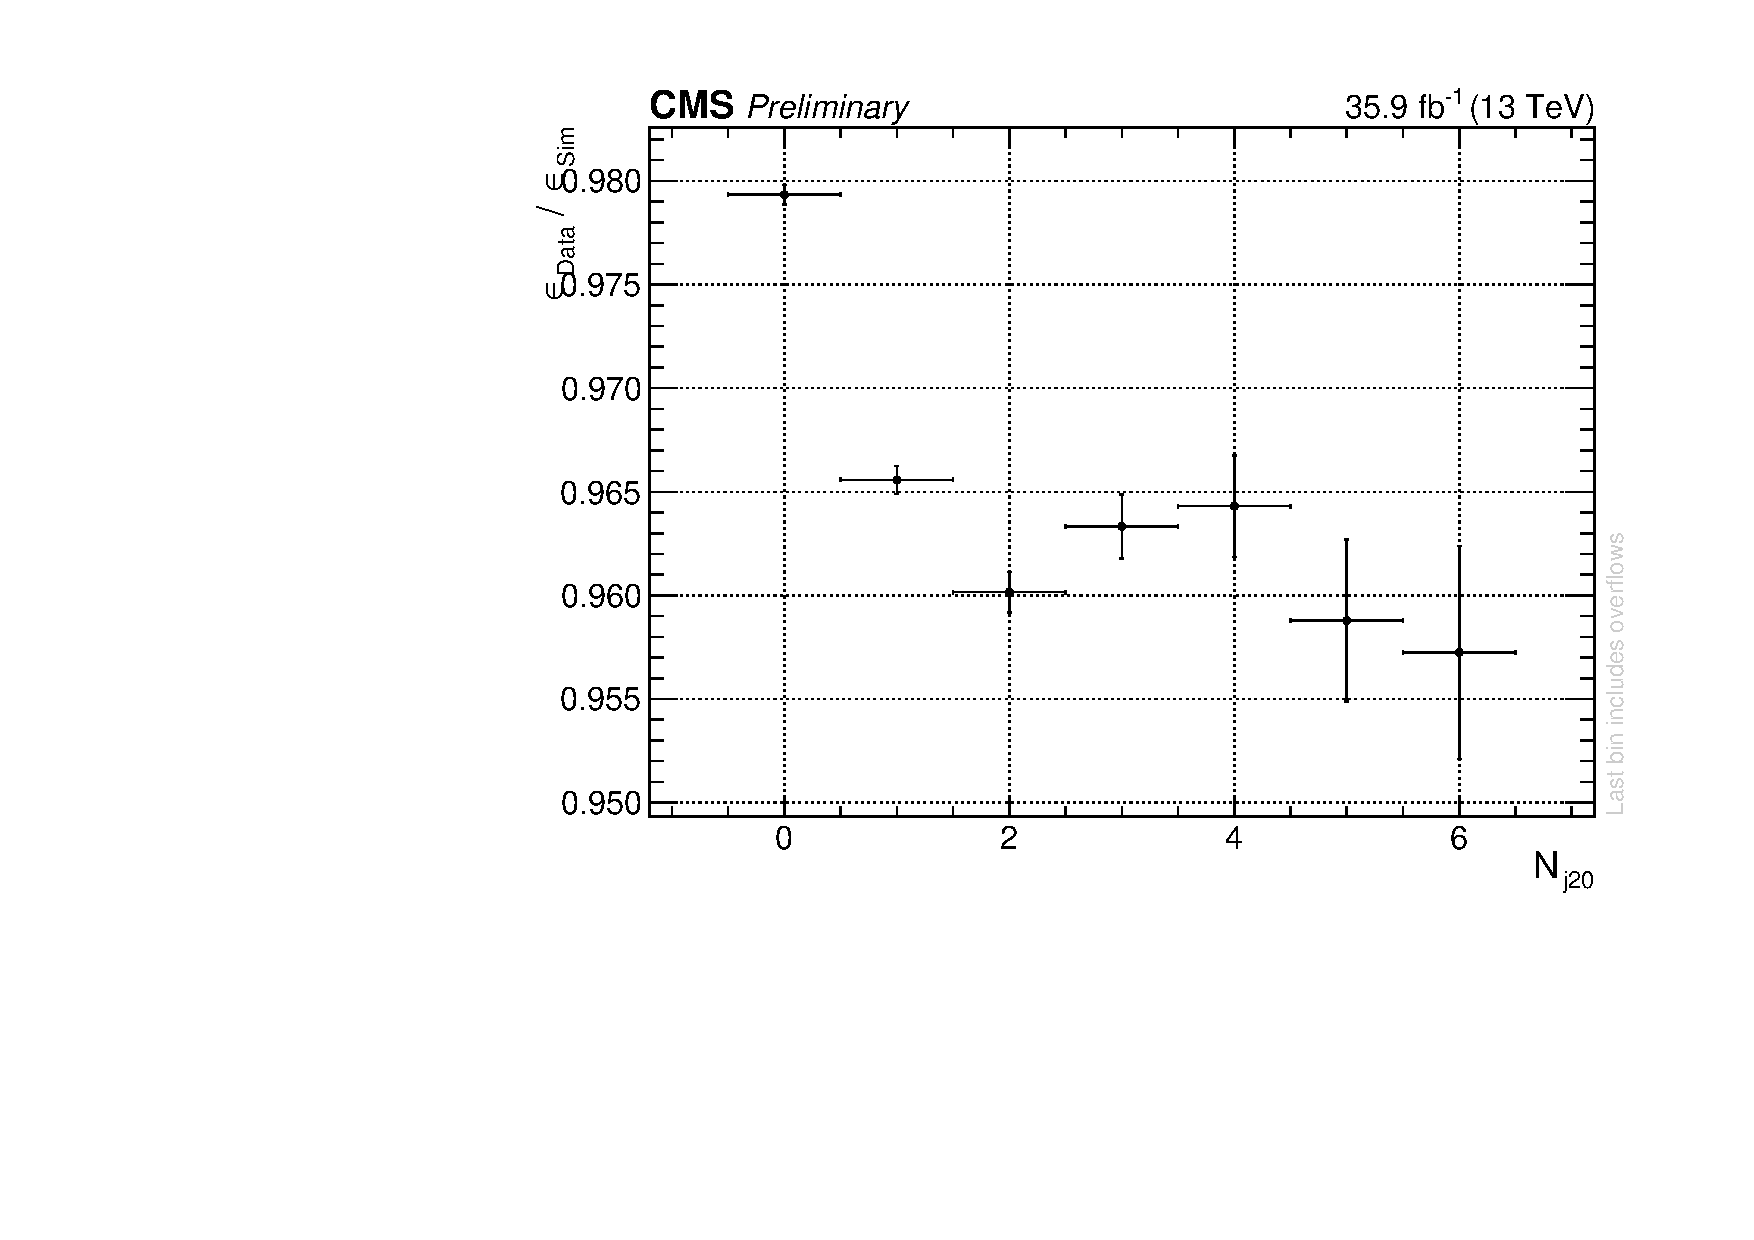
\includegraphics[width=0.45\textwidth]{fig/chapt7/trigger_eff/sf_jets.pdf}
  \caption{Trigger efficiencies in data and Drell--Yan simulation and their ratios as a function of $p_{T}$ of the ``probe'', pseudorapidity of the associated ECAL supercluster, number of reconstructed primary vertices, and number of jets with $p_{T} > 20$~GeV. Statistical uncertainties are shown.}
  \label{Fig:TnP1DEff}
\end{figure}

Two-dimensional scale factors used in this search are shown in Fig.~\ref{Fig:TnP2DSF}, together with their full uncertainties.
Main components of the uncertainties are shown in Fig.~\ref{Fig:TnP2DSFUnc} and represent the statistical uncertainty (in both data and simulation) and two systematic shifts.
The first systematic uncertainty accounts for the change in the scale factors when the mass window is tightened to $70 < m_{ee} < 110$~GeV.
The second one is induced by increasing the $p_{T}$~threshold in the definition of the ``tag'' to $p_{T} > 45$~GeV.
These three sources are summed up in quadrature, together with a 2\%~uncertainty to cover for the dependence on jet multiplicity and an additional 1\%~uncertainty for unaccounted effects.

\begin{figure}
\centering
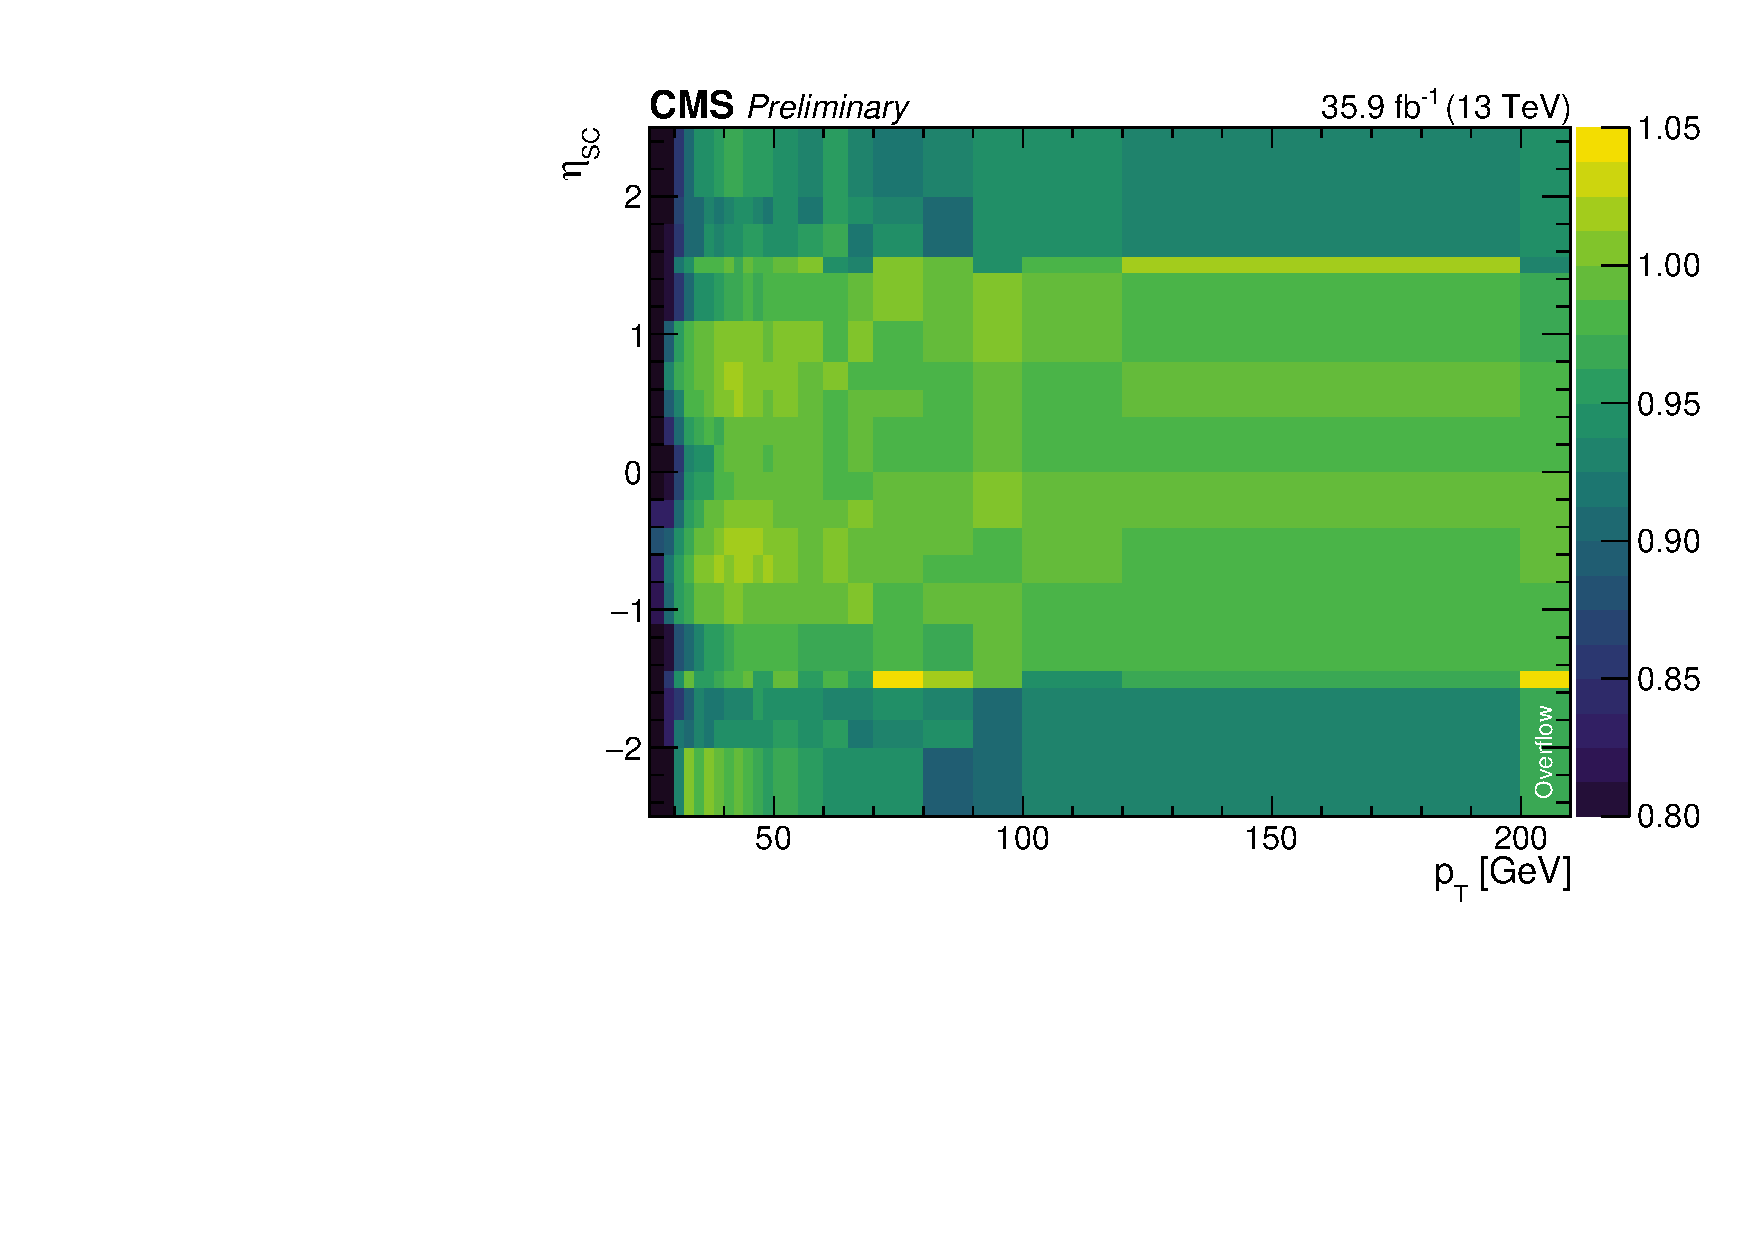
\includegraphics[width=0.45\textwidth]{fig/chapt7/trigger_eff/sf2d_nominal}
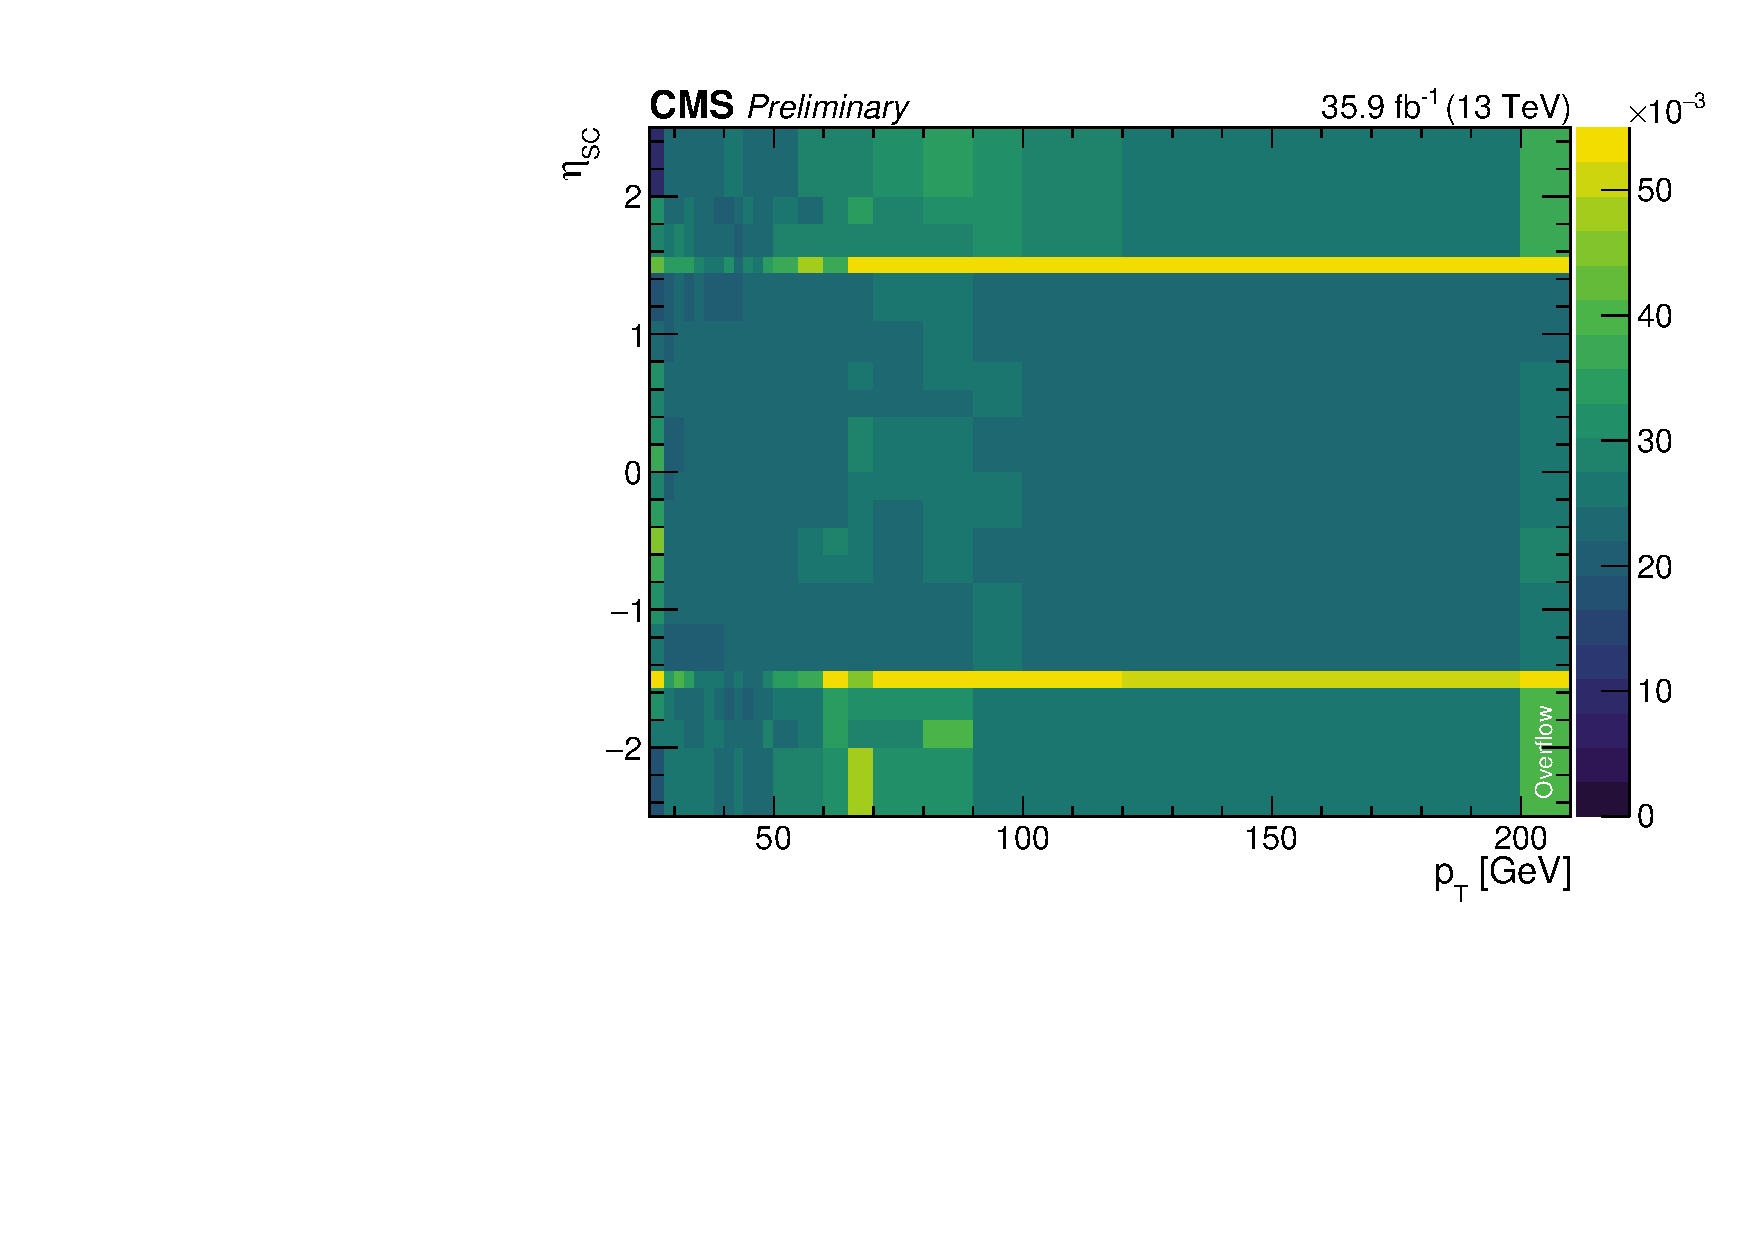
\includegraphics[width=0.45\textwidth]{fig/chapt7/trigger_eff/sf2d_fullError}
\caption{Trigger scale factors as a function of $p_{T}$ and $\eta_\text{SC}$ (left) and their full uncertainties (right).}
\label{Fig:TnP2DSF}
\end{figure}

\begin{figure}
  \centering
  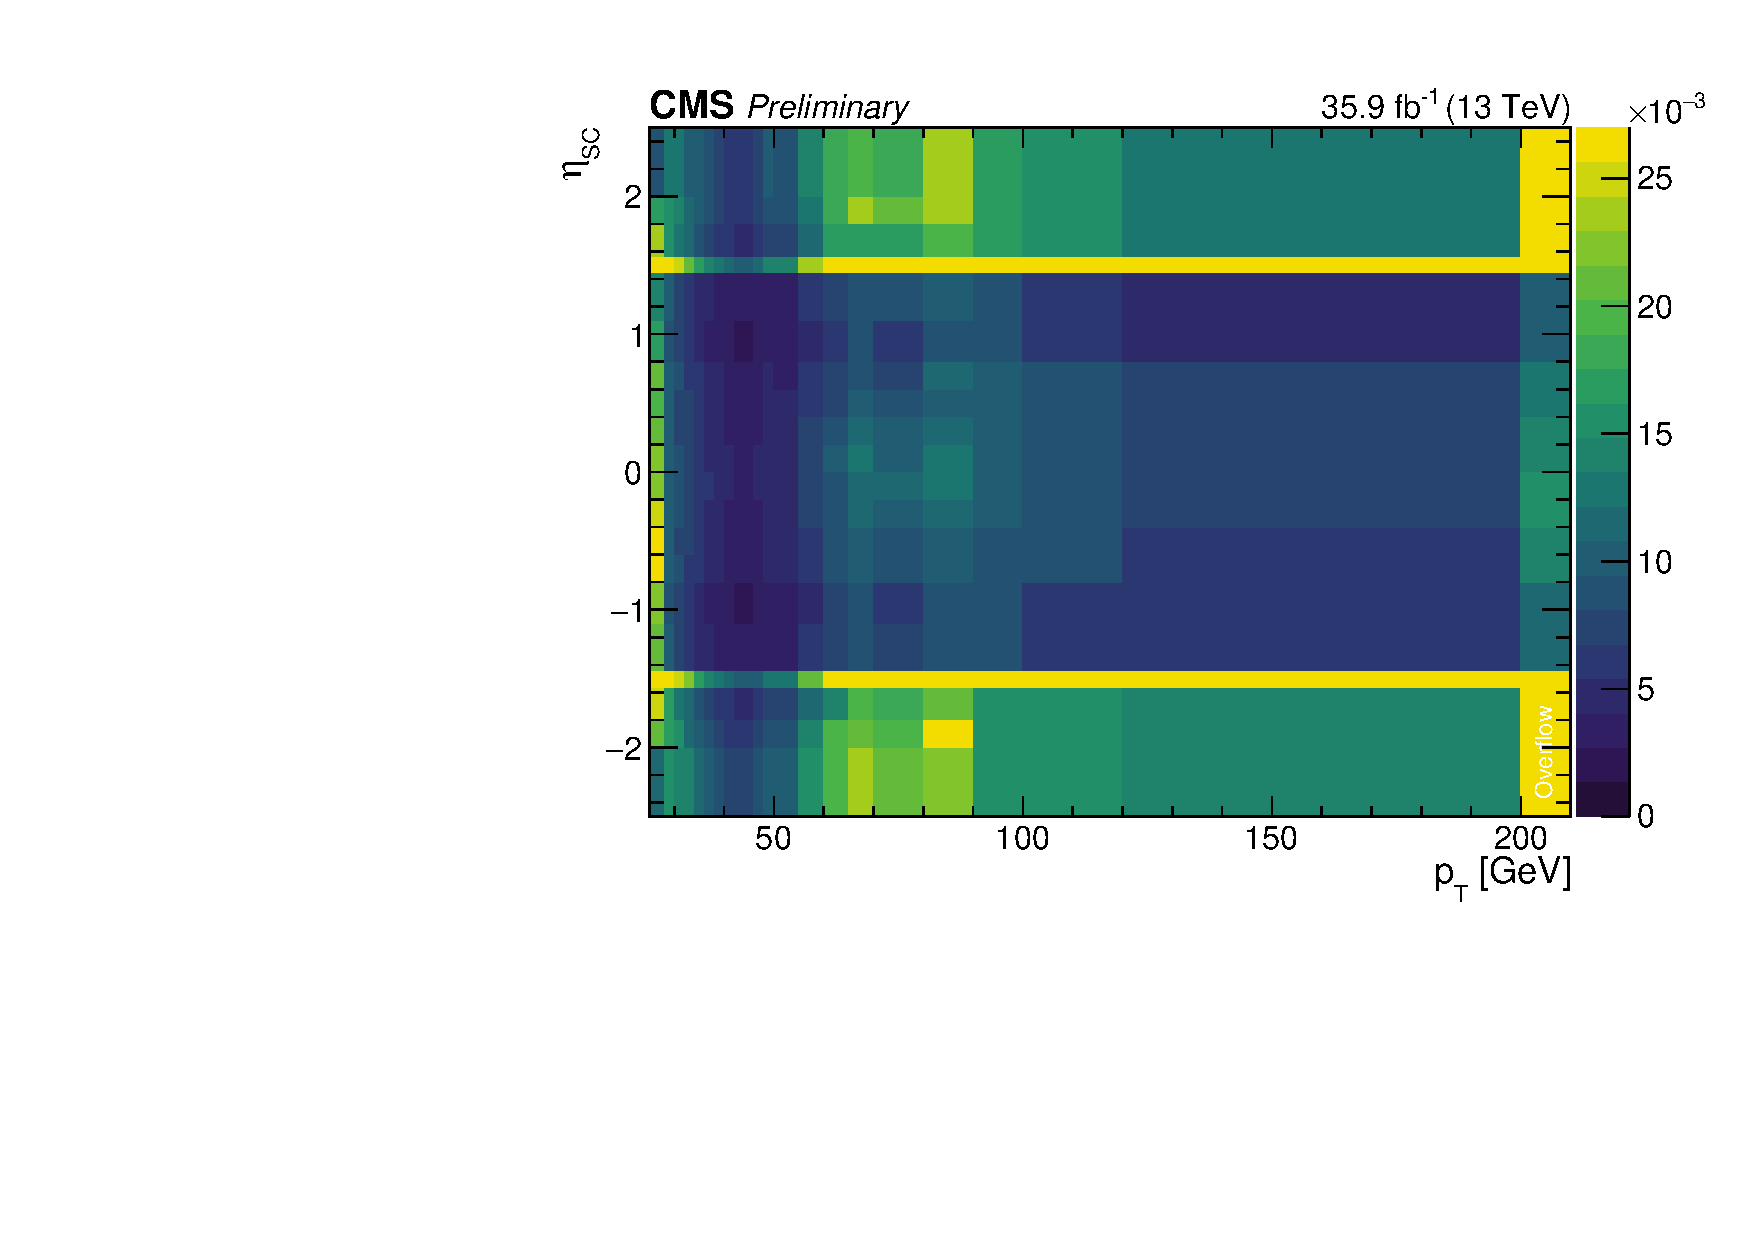
\includegraphics[width=0.32\textwidth]{fig/chapt7/trigger_eff/sf2d_statError}
  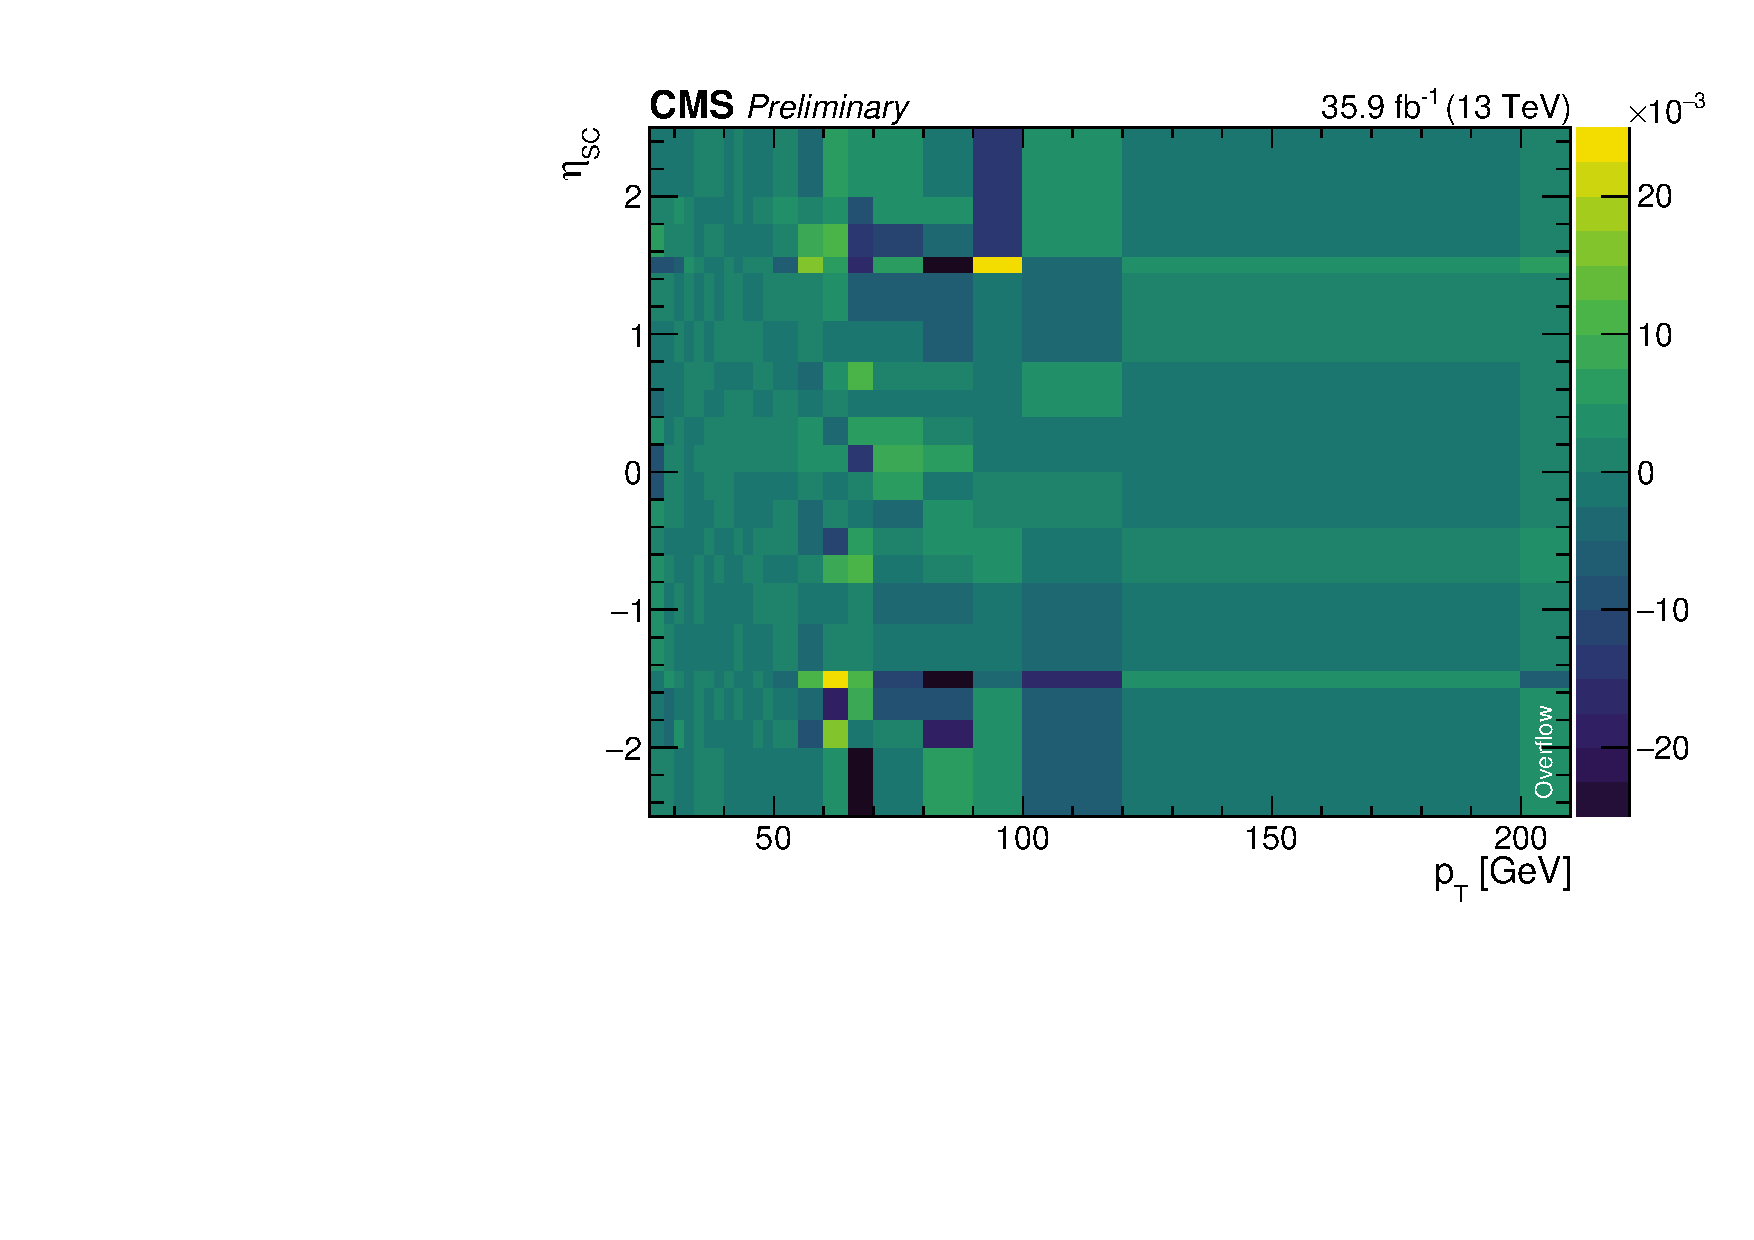
\includegraphics[width=0.32\textwidth]{fig/chapt7/trigger_eff/sf2d_diffMassWindow}
  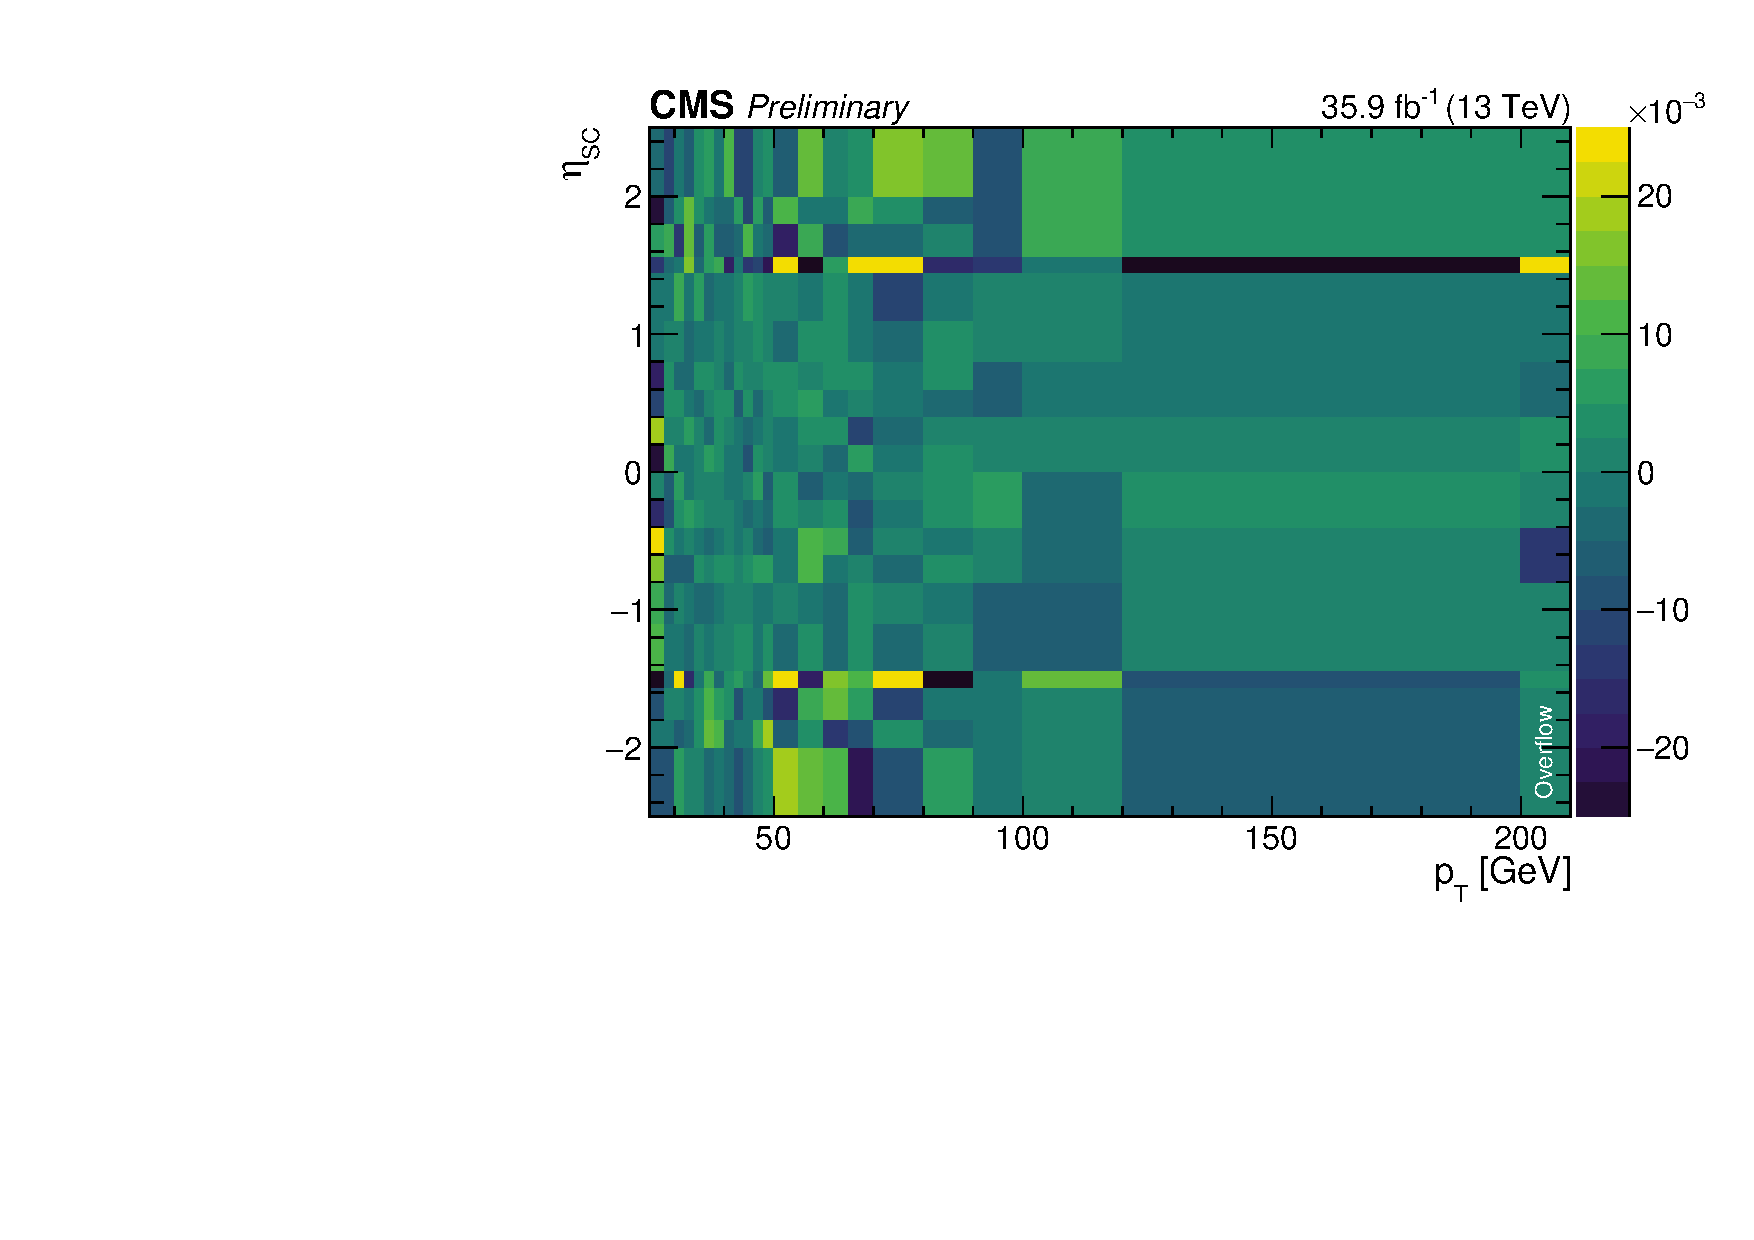
\includegraphics[width=0.32\textwidth]{fig/chapt7/trigger_eff/sf2d_diffTagPt}
  \caption{Components of uncertainties of the two-dimensional trigger scale factors: statistical uncertainty~(left), absolute difference due to the variation of the $m_{ee}$ window~(middle) and the $p_{T}$ of the ``tag''~(right).}
  \label{Fig:TnP2DSFUnc}
\end{figure}

\noindent \textbf{Muon trigger efficiency}: An inclusive~\textit{or} trigger of \texttt{HLT\_IsoMu24\_v*} and \texttt{HLT\_IsoTkMu24\_v*} triggers are used for muon selection in this analysis. The efficiencies scale factors are provided centrally as a function of $p_T$ and $\eta$ of the muons using the tag-and-probe method as discussed in the above Sec.~\ref{subsec:elec_trigg}. A detail study is given in the presentation here~\cite{wiki:muon_trigger} while Fig.~\ref{Fig:muon_trigg_eff} shows the trigger efficiencies as a function of $p_T$ and $\eta$, left to right.
\begin{figure}
  \centering
  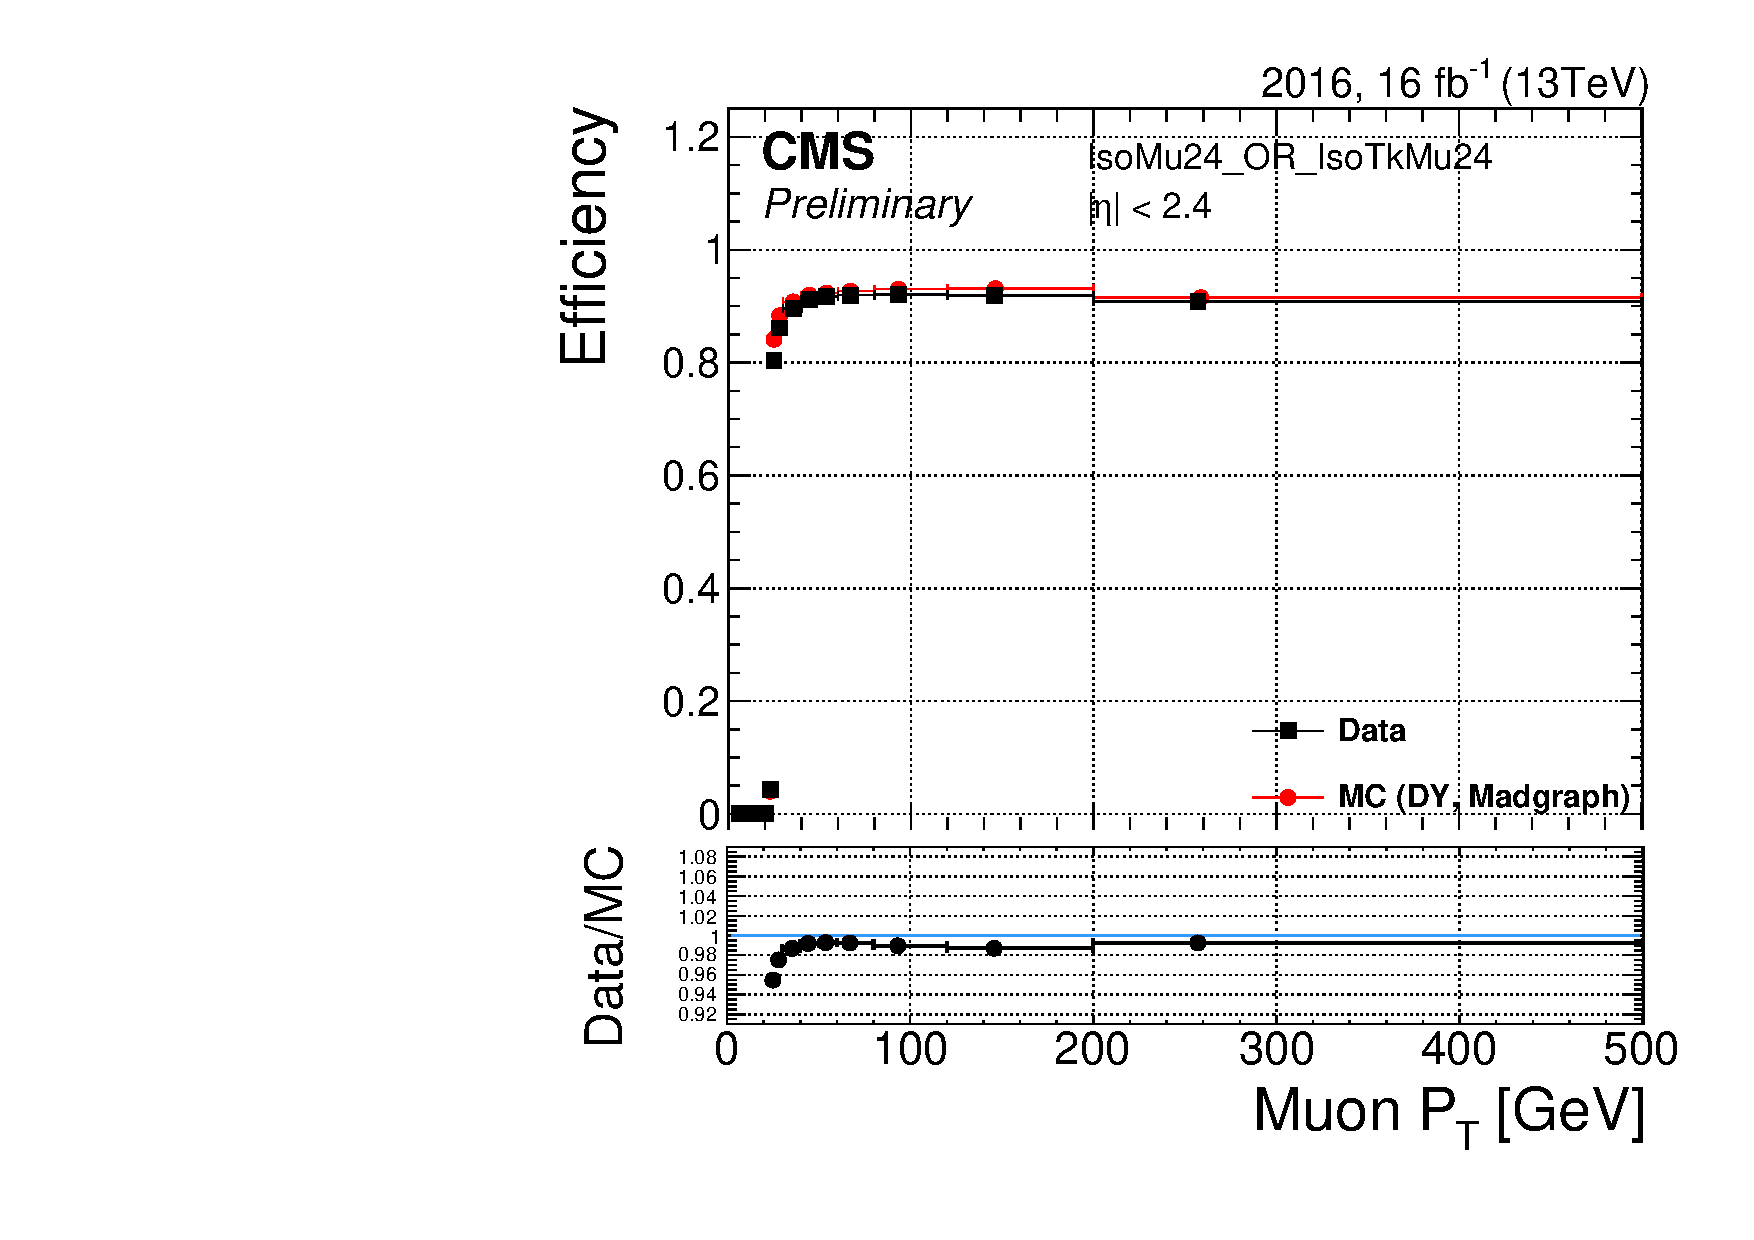
\includegraphics[width=0.45\textwidth]{fig/chapt7/trigger_eff/Total_IsoTkMu24_pt}
  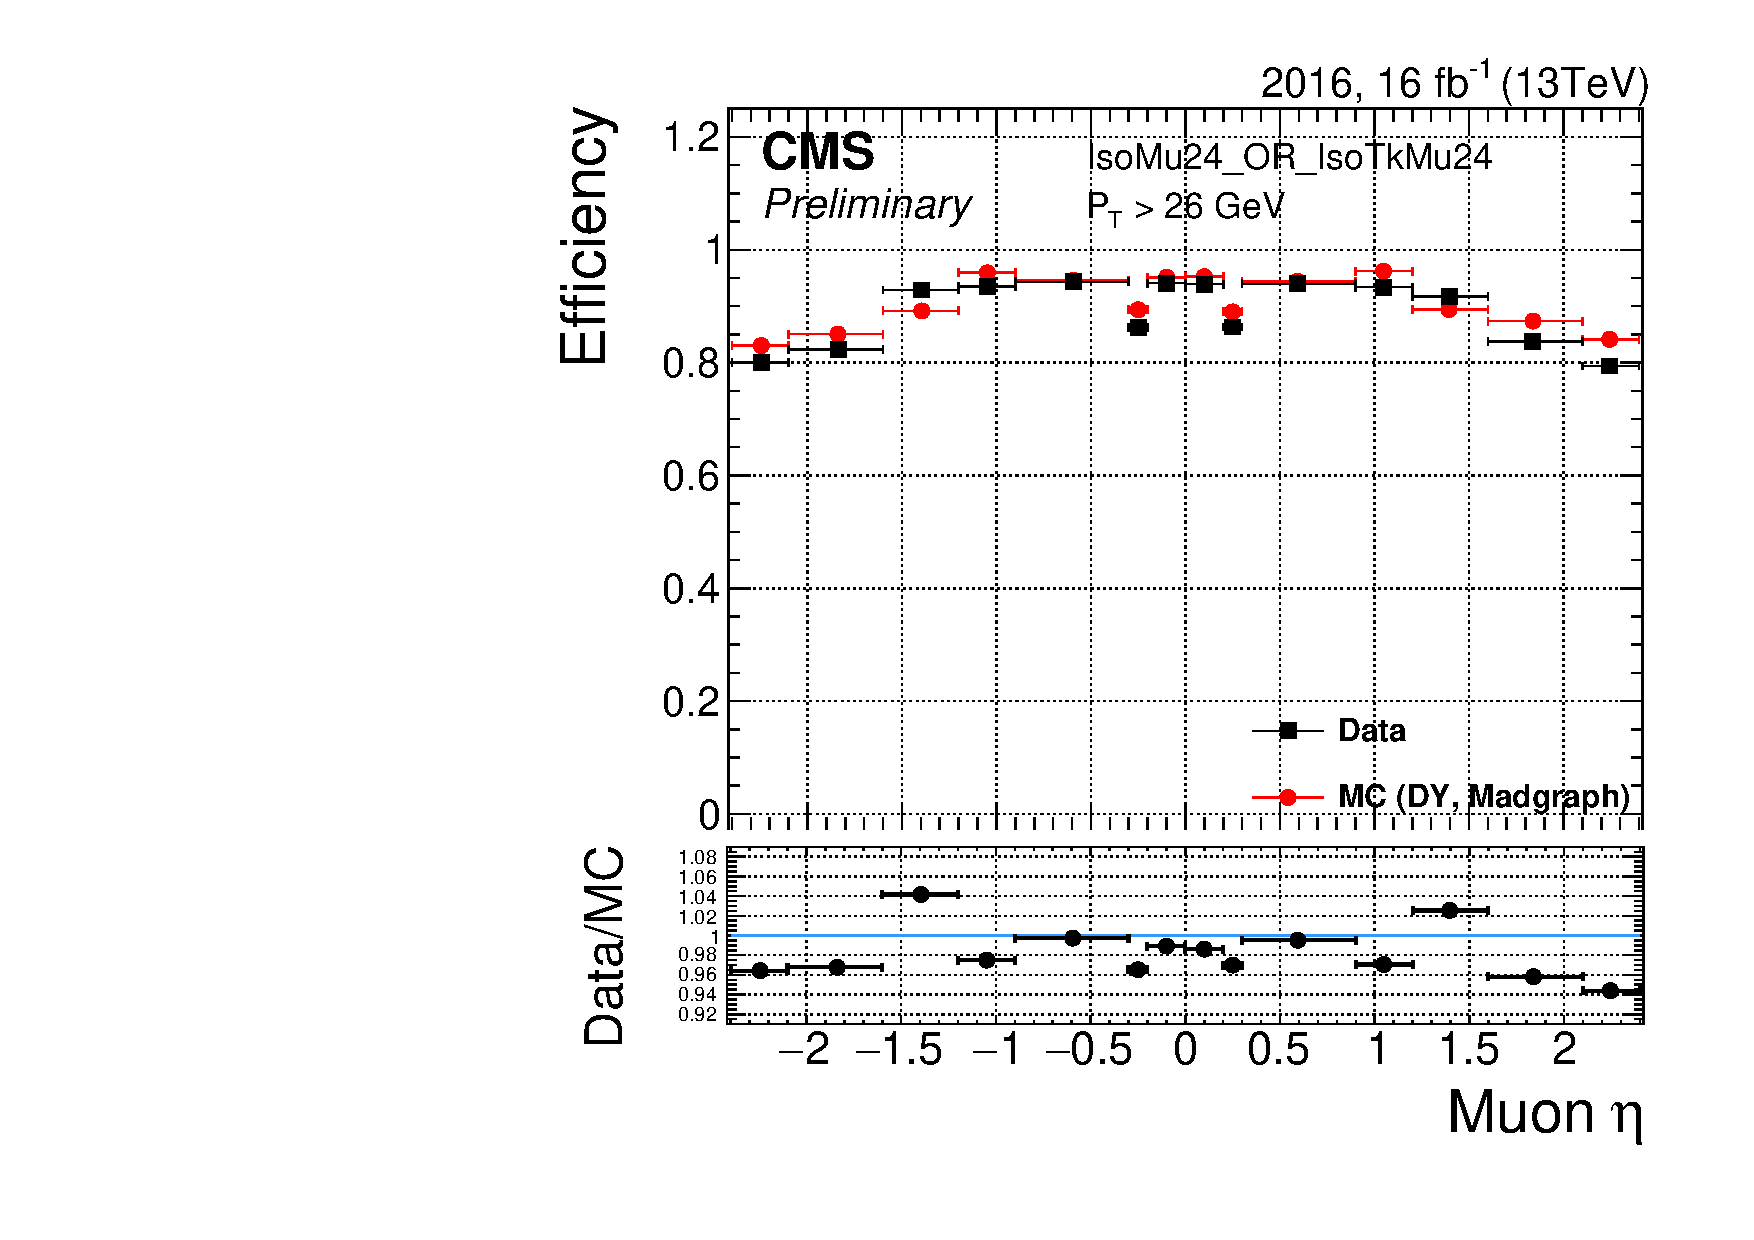
\includegraphics[width=0.45\textwidth]{fig/chapt7/trigger_eff/Total_IsoTkMu24_eta}
  \caption{Efficiencies of the muon trigger with $OR$ combination of triggers \texttt{HLT\char`_IsoMu24\char`_v*} and \texttt{HLT\char`_IsoTkMu24\char`_v*}: as a function of muon $p_T$, left and $\eta$ on right~\cite{wiki:muon_trigg_eff}.}
  \label{Fig:muon_trigg_eff}
\end{figure}  
\subsection{Muon and electron efficiency scale factors}
\label{Sec:LeptonSF}
%
Electrons and muons efficiencies scale factors for all other aspects of reconstruction are officially provided, except of the electron trigger scale factors discussed above.
All these measurements have also been performed with the tag-and-probe method.

Corrections for muons are taken from Ref.~\cite{Wiki:MuonSF}.
They include data-to-simulation scale factors for efficiencies of inclusive~\textit{or} of triggers \texttt{HLT\char`_IsoMu24\char`_v*} and \texttt{HLT\char`_IsoTkMu24\char`_v*}, track reconstruction, tight working point of the identification algorithm, and tight selection on isolation.
The correction for the efficiency of track reconstruction depends on the pseudorapidity of the muon, while all other scale factors are parameterized with $p_{T}$ and $|\eta|$ of the muon.
Whenever the scale factors are provided separately for different data-taking periods, they are combined assigning each measurement a weight that is proportional to the respective integrated luminosity. Plot~\ref{fig:lepidiso_correction}(b) is corrected by muon ID and isolation scale factors and in plot~\ref{fig:lepidiso_correction}(a) they are not applied.

In the electron channel this search makes use of scale factors for track reconstruction efficiency and the efficiency of the tight working point of the cut-based identification algorithm.
They are provided in Ref.~\cite{Wiki:ElectronSF} as functions of $\eta_\text{SC}$ and $(p_{T}, \eta_\text{SC})$ respectively. Although the scale factors for electron identification were computed with no selection on impact parameters, it has been demonstrated~\cite{Talk:EleSFImpactParameters} that they are applicable also for electrons defined as in Sec.~\ref{Sec:Reconstruction}.


\begin{figure}[htp]
\centering
\begin{tabular}{cc}
\hspace{-0.5cm}
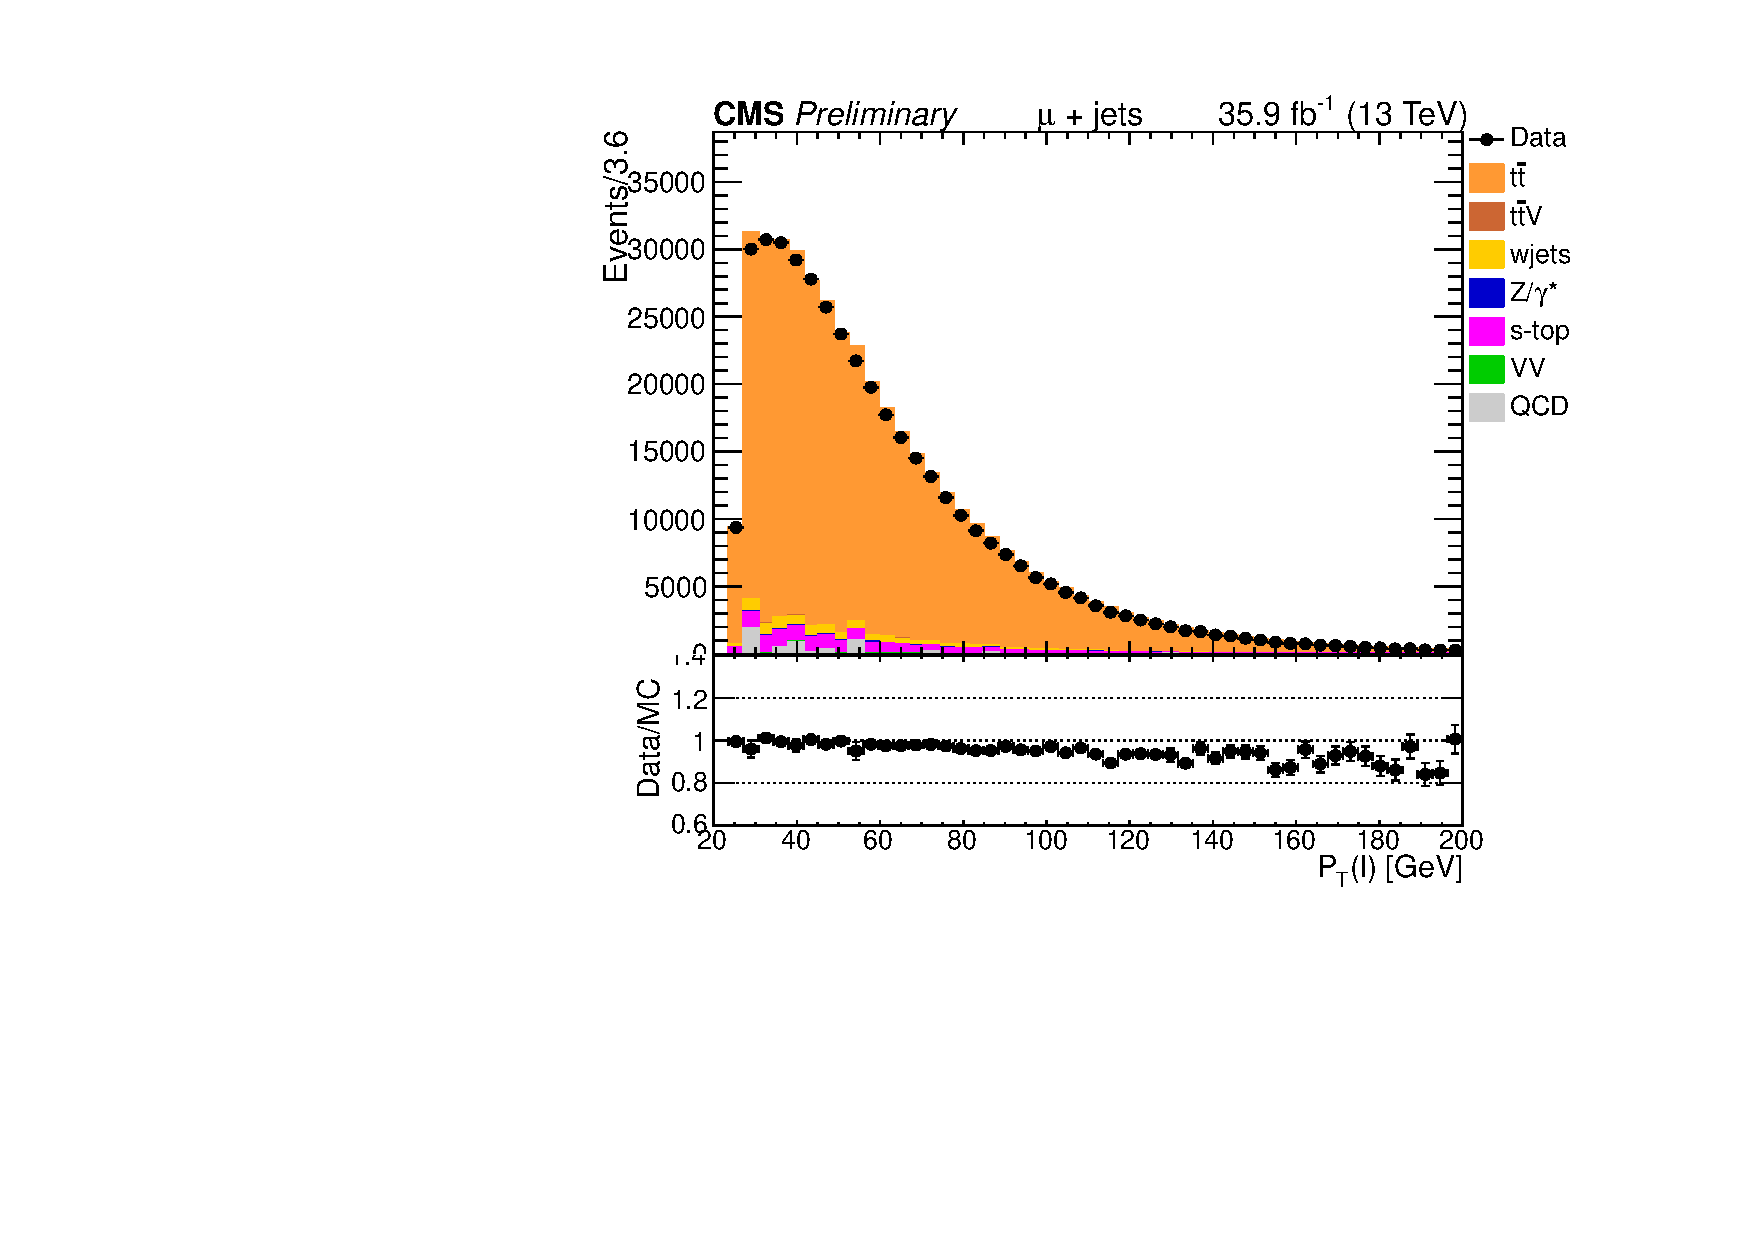
\includegraphics[scale=0.45]{fig/chapt7/correction/id_iso_nocorrection_Pt_lep.pdf}
& \hspace{-1.50cm} 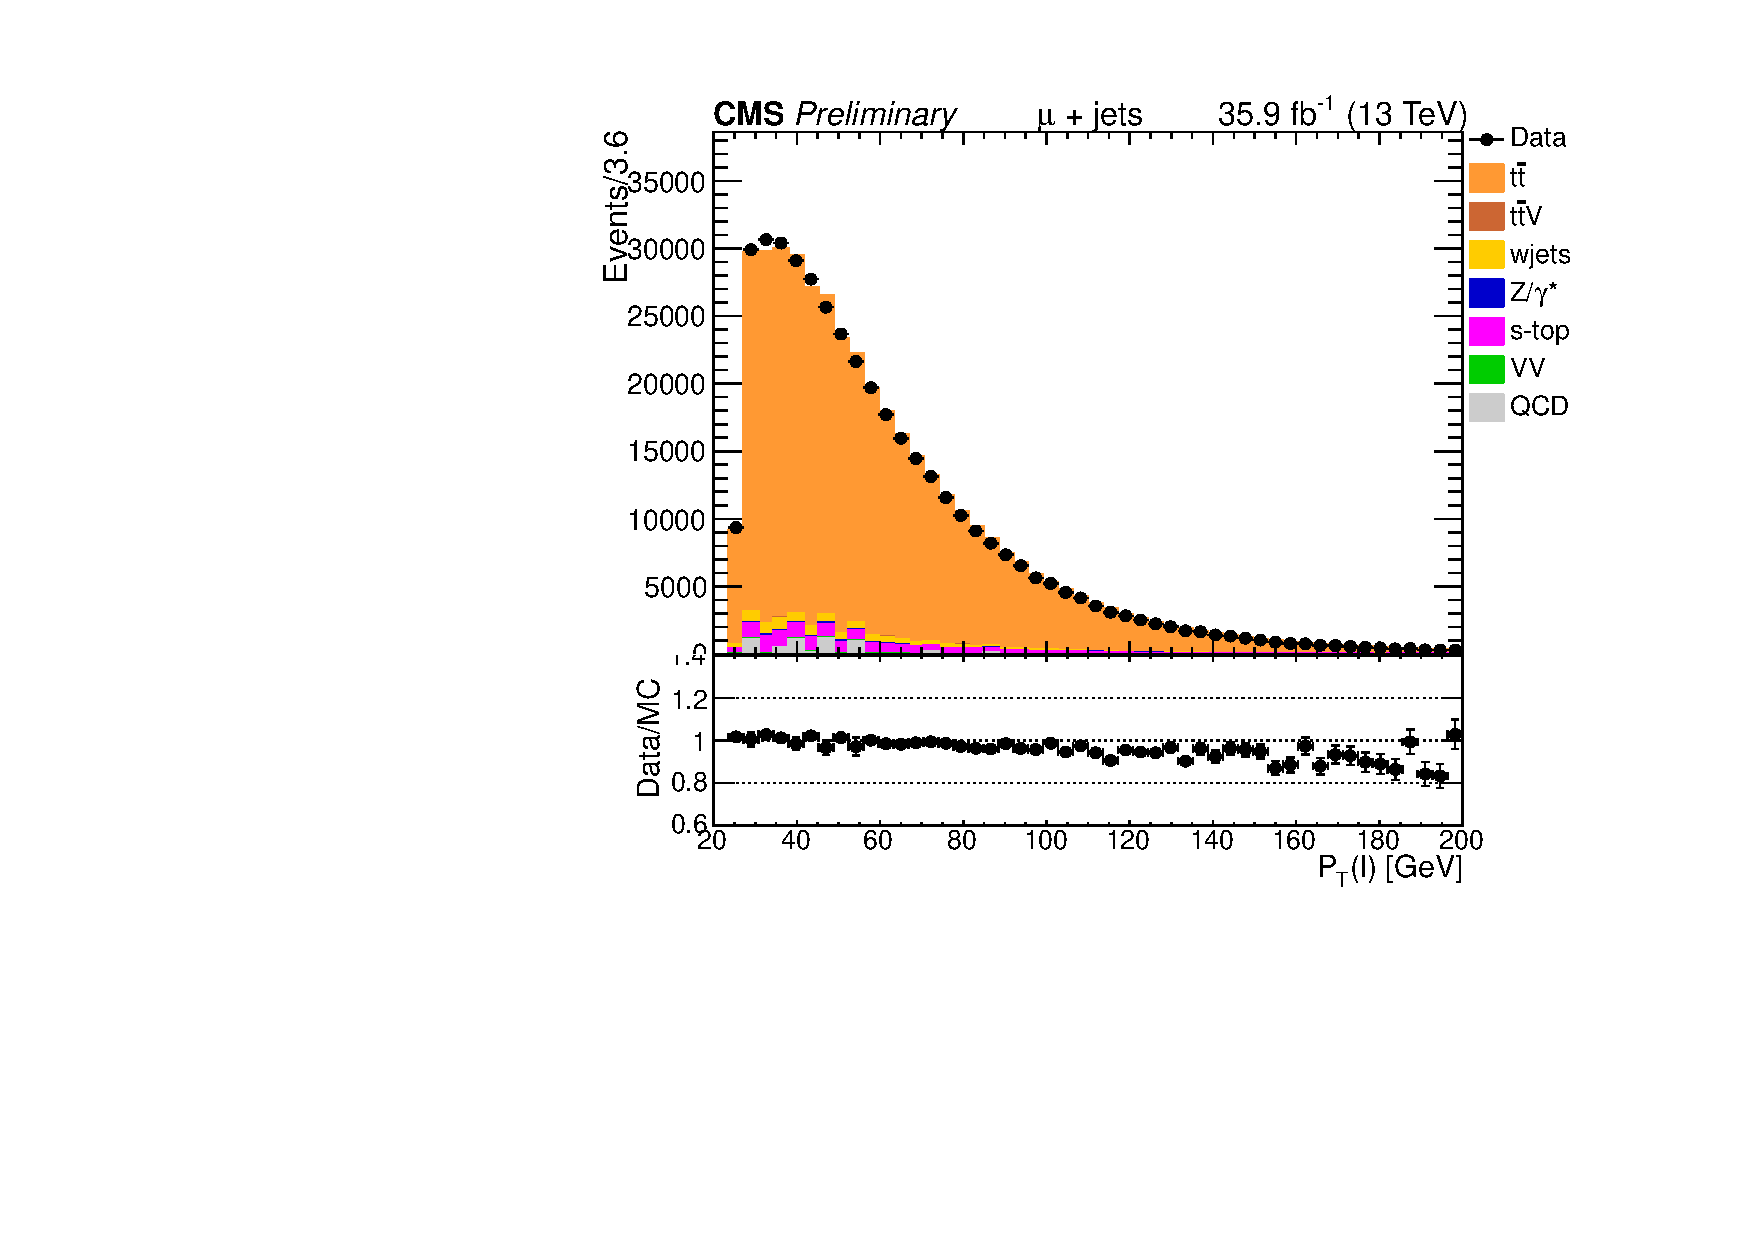
\includegraphics[scale=0.45]{fig/chapt7/correction/id_iso_corrected_Pt_lep.pdf}\\
  \qquad ($\mathbf{a}$)\qquad\qquad&($\mathbf{b}$)\qquad\qquad\qquad\qquad \\
\end{tabular}
\caption{Transverse momentum of muon in data and MC pre (a) and post (b) ID and Isolation correction in the $t\bar{t}$ dominated region.}\label{fig:lepidiso_correction}
\end{figure}

\subsection{Generator level weights}
\label{sec:genweights}
 Simulation processes are scaled according to the integrated luminosity using the following formula.
 \begin{equation}
 N = \mathcal{L} * \sigma
\end{equation}  
where $\mathcal{L}$ is the integrated luminosity, $\sigma$ is the theoretical prediction N is the generated number of events.
\subsection{Correction of $p_{T}$ spectrum of top quarks in $t\bar{t}$ events}
\label{Sec:TopPtReweighting}
%
It is known that available event generators do not describe distributions of transverse momenta of top quarks in the SM $t\bar t$ production~\cite{Khachatryan:2015oqa, Khachatryan:2015fwh, Khachatryan:2016mnb, CMS-PAS-TOP-16-007}.
In particular, the combination of $\textsc{POWHEG}$~V2 and $\textsc{PYTHIA}$~8 used in this search predicts an overall harder spectrum than observed in data.
The origin of this discrepancy is not understood, and uncovering it will likely require a substantial effort from the theory community.
At the same time it has a significant impact on the majority of analyses involving SM~$t\bar{t}$ and affects $p_{T}$~distributions of various reconstructed objects, not only the top quarks but also their decay products.

In order to correct for the discrepancy, an empirical reweighting based on the observed $p_{T}$~distributions of top quarks~\cite{Wiki:TopPtReweighting} is utilized.
It is only applied to the SM $t\bar{t}$~production.
Event weights are evaluated as a function of the transverse momenta of the last top quarks found in the event history (i.e. after the modelling of the final state radiation):
\begin{linenomath}
\begin{equation}
 \label{Eq:TopPtWeight}
 w\!\left(p_{T}^{(1)}, p_{T}^{(2)}\right) = \sqrt{\prod_{i = 1}^2 \exp\!\left(p_0 + p_1 \cdot p_{T}^{(i)}\right)} = \exp\!\left(p_0 + p_1 \cdot \frac{p_{T}^{(1)} + p_{T}^{(2)}}{2}\right).
\end{equation}
\end{linenomath}
Parameters of the reweighting are computed as
\begin{linenomath}
\begin{equation}
 \label{Eq:TopPtWeightParams}
 \begin{aligned}
  p_0 &= 6.15024\times 10^{-2} + 3.243 \times 10^{-2} \cdot \nu_1 - 4.353\times 10^{-7} \cdot \nu_2 \\
  p_1 &= -5.17833\times 10^{-4} - 1.404\times 10^{-4} \cdot \nu_1 - 1.005\times 10^{-4} \cdot \nu_2,
 \end{aligned}
\end{equation}
\end{linenomath}
where $\nu_1$ and $\nu_2$ are independent nuisance parameters distributed according to the standard normal distribution $\mathcal N(0, 1)$.
These nuisance parameters reflect uncertainties of the fit of the unfolded top quark's~$p_{T}$ spectrum.
Factors in front of $\nu_{1,\,2}$ have been obtained by finding a linear transformation that transforms the covariance matrix of the fit~\cite{HN:TopPtCovariance} into an identity one.
Nominal weights are computed by setting $(\nu_1, \nu_2) = (0, 0)$, while two pairs of independent systematic variations are given by values $(\pm 1, 0)$ and $(0, \pm 1)$.

The empirical reweighting has been constructed from the normalized differential cross section $1/\sigma \cdot \mathrm d\sigma / \mathrm dp_{T}$ and as such should only change the shape of the distribution but not the overall yield.
To enforce this condition, weights given by Eq.~\ref{Eq:TopPtWeight} are additionally divided by their mean values computed over the full $t\bar t$ dataset with no event selection.
These values are reported in Table~\ref{Tab:TopPtMeanWeights} for all considered variations.

\begin{table}
  \centering
  \caption{Mean values of weights given by Eqs.~\ref{Eq:TopPtWeight}, \ref{Eq:TopPtWeightParams} with no event selection.}
  \label{Tab:TopPtMeanWeights}
  \begin{tabular}{cc}
  \hline
  \hline
  Nuisances $(\nu_1, \nu_2)$  & Mean weight \\
  \hline
  $(0, 0)$   & 0.9985 \\
  $(+1, 0)$  & 1.0142 \\
  $(-1, 0)$  & 0.9832 \\
  $(0, +1)$  & 0.9865 \\
  $(0, -1)$  & 1.0107 \\
  \hline
  \hline
  \end{tabular}
\end{table}
The effect of the reweighting is demonstrated in Fig.~\ref{Fig:TopPtReweighting}, which shows distributions of the $p_{T}$ of the reconstructed top quarks, the mass of the $t\bar t$~system, and the angular observable used in this analysis, $\cos\theta^{\star}_{t_{l}}$, in the signal region.
Definition of the signal region and the reconstruction of the $t\bar t$~system will be described in dedicated sections below.
The results are compared against a reweighting to differential distributions computed with NNLO QCD + NLO EW precision~\cite{Czakon:2017wor}.
The corresponding event weights have been obtained as the ratio between the theoretical differential distributions and distributions of the last top quarks in the event history in the used $t\bar t$~datasets before any event selection, both normalized to the same cross section.
Theoretical results are not available for the angular variable.
As can be seen from the figure, both reweightings improve the modelling of the top quarks'~$p_{T}$ distributions, while for $m_{tt}$ using the theoretical distribution leads to a significantly worse description.
This does not necessarily indicate a problem in the theoretical computation because the matching between definitions of top quarks in the $\textsc{POWHEG}$ + $\textsc{PYTHIA}$ sample and the stable top quarks from Ref.~\cite{Czakon:2017wor} is not a well-posed problem, and using different definitions of top quarks might affect the distributions.
The empirical reweighting, on the other hand, gives a sufficiently good description of all the four observables and, as a direct result of the change in the distributions of top quarks'~$p_{T}$, also improves modelling of the transverse momenta of leptons, jets, and $p_{T}^{miss}$.
Figure~\ref{Fig:TopPtReweighting} shows a remaining discrepancy in the low-energy region, but, at least in part, it can be attributed to an underestimation of the multijet background.
It is described with a data-driven method, as will be discussed in Sec.~\ref{Sec:DataDrivenQCD}, and a conservative uncertainty of ${+100} / {-50}$\% is assigned for its normalization.
The impact of this uncertainty is also shown in the figure, and it covers for a part of the discrepancy.
\begin{figure}
  \centering
  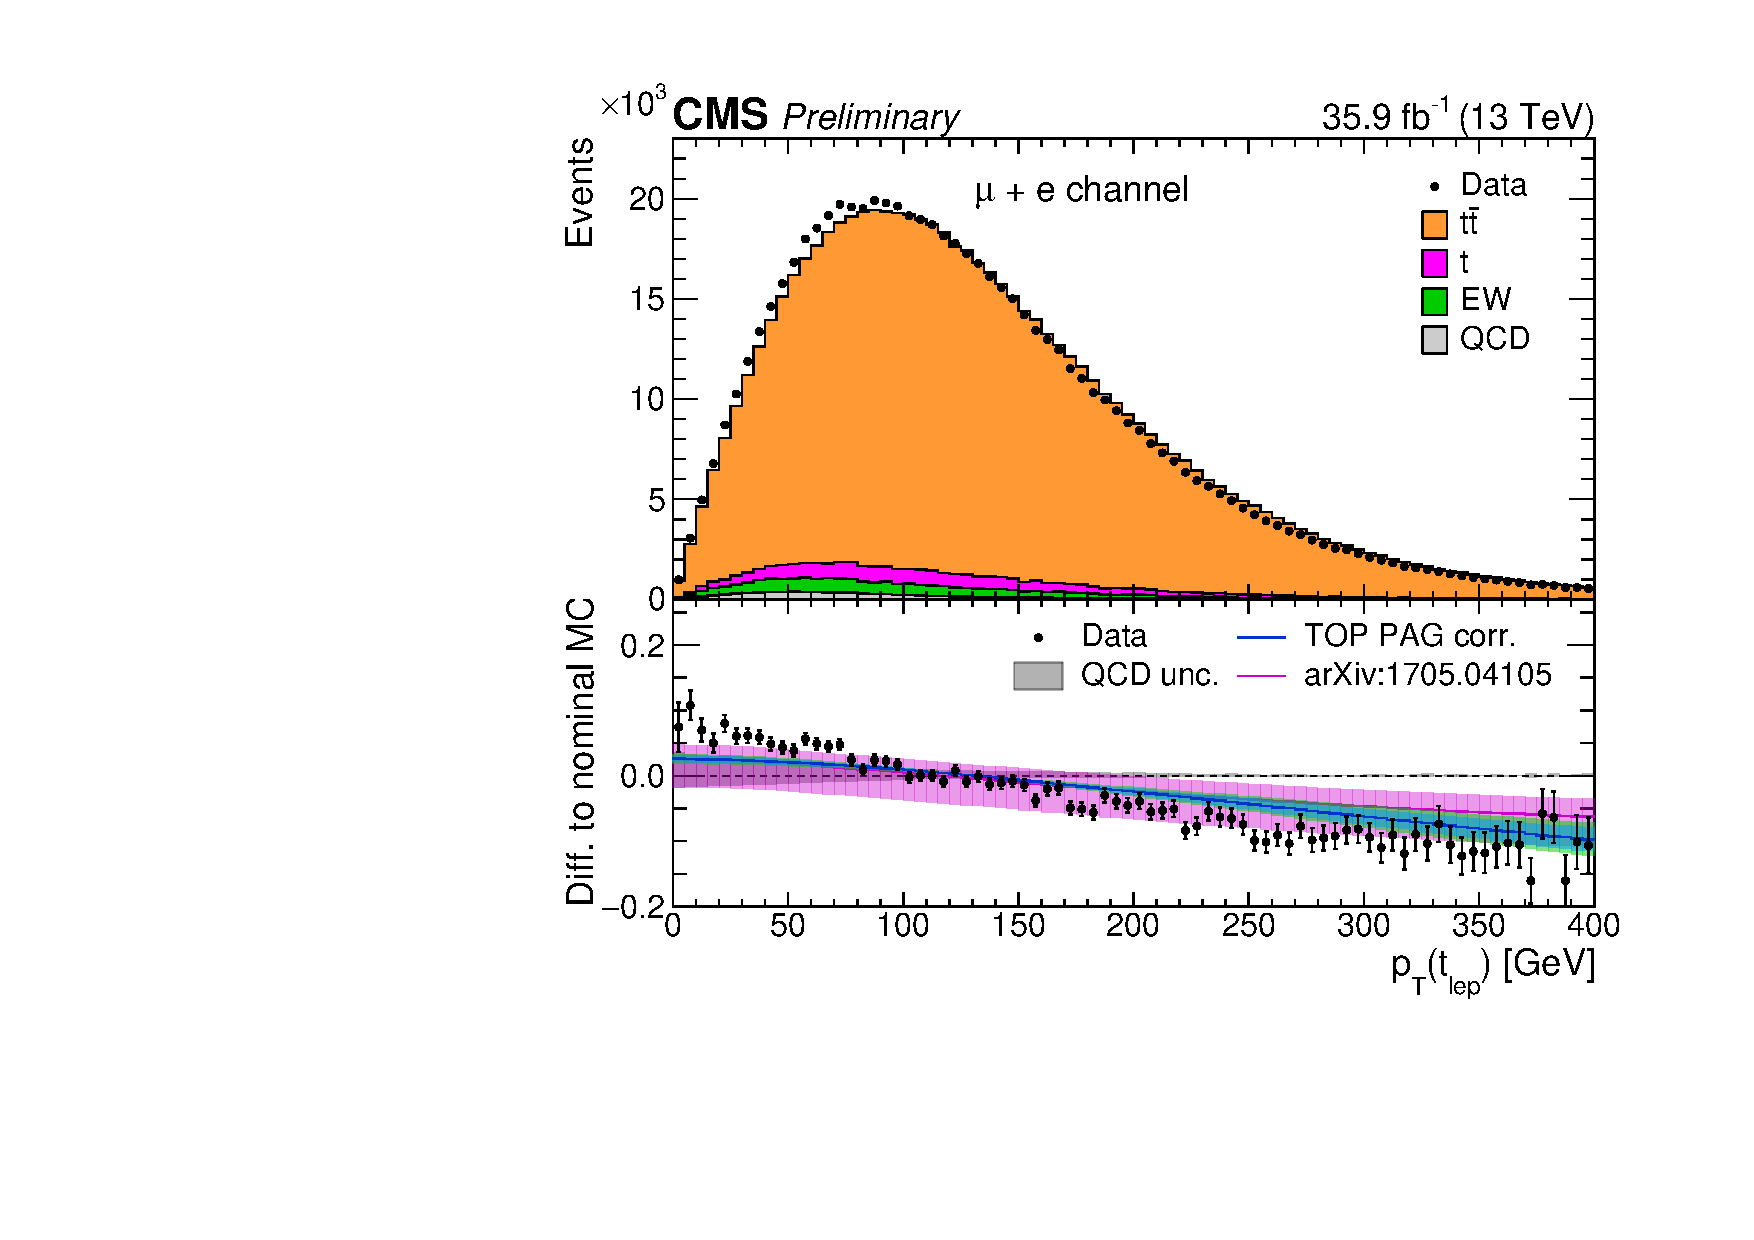
\includegraphics[width=0.45\textwidth]{fig/chapt7/correction/PtTopLep.pdf}
  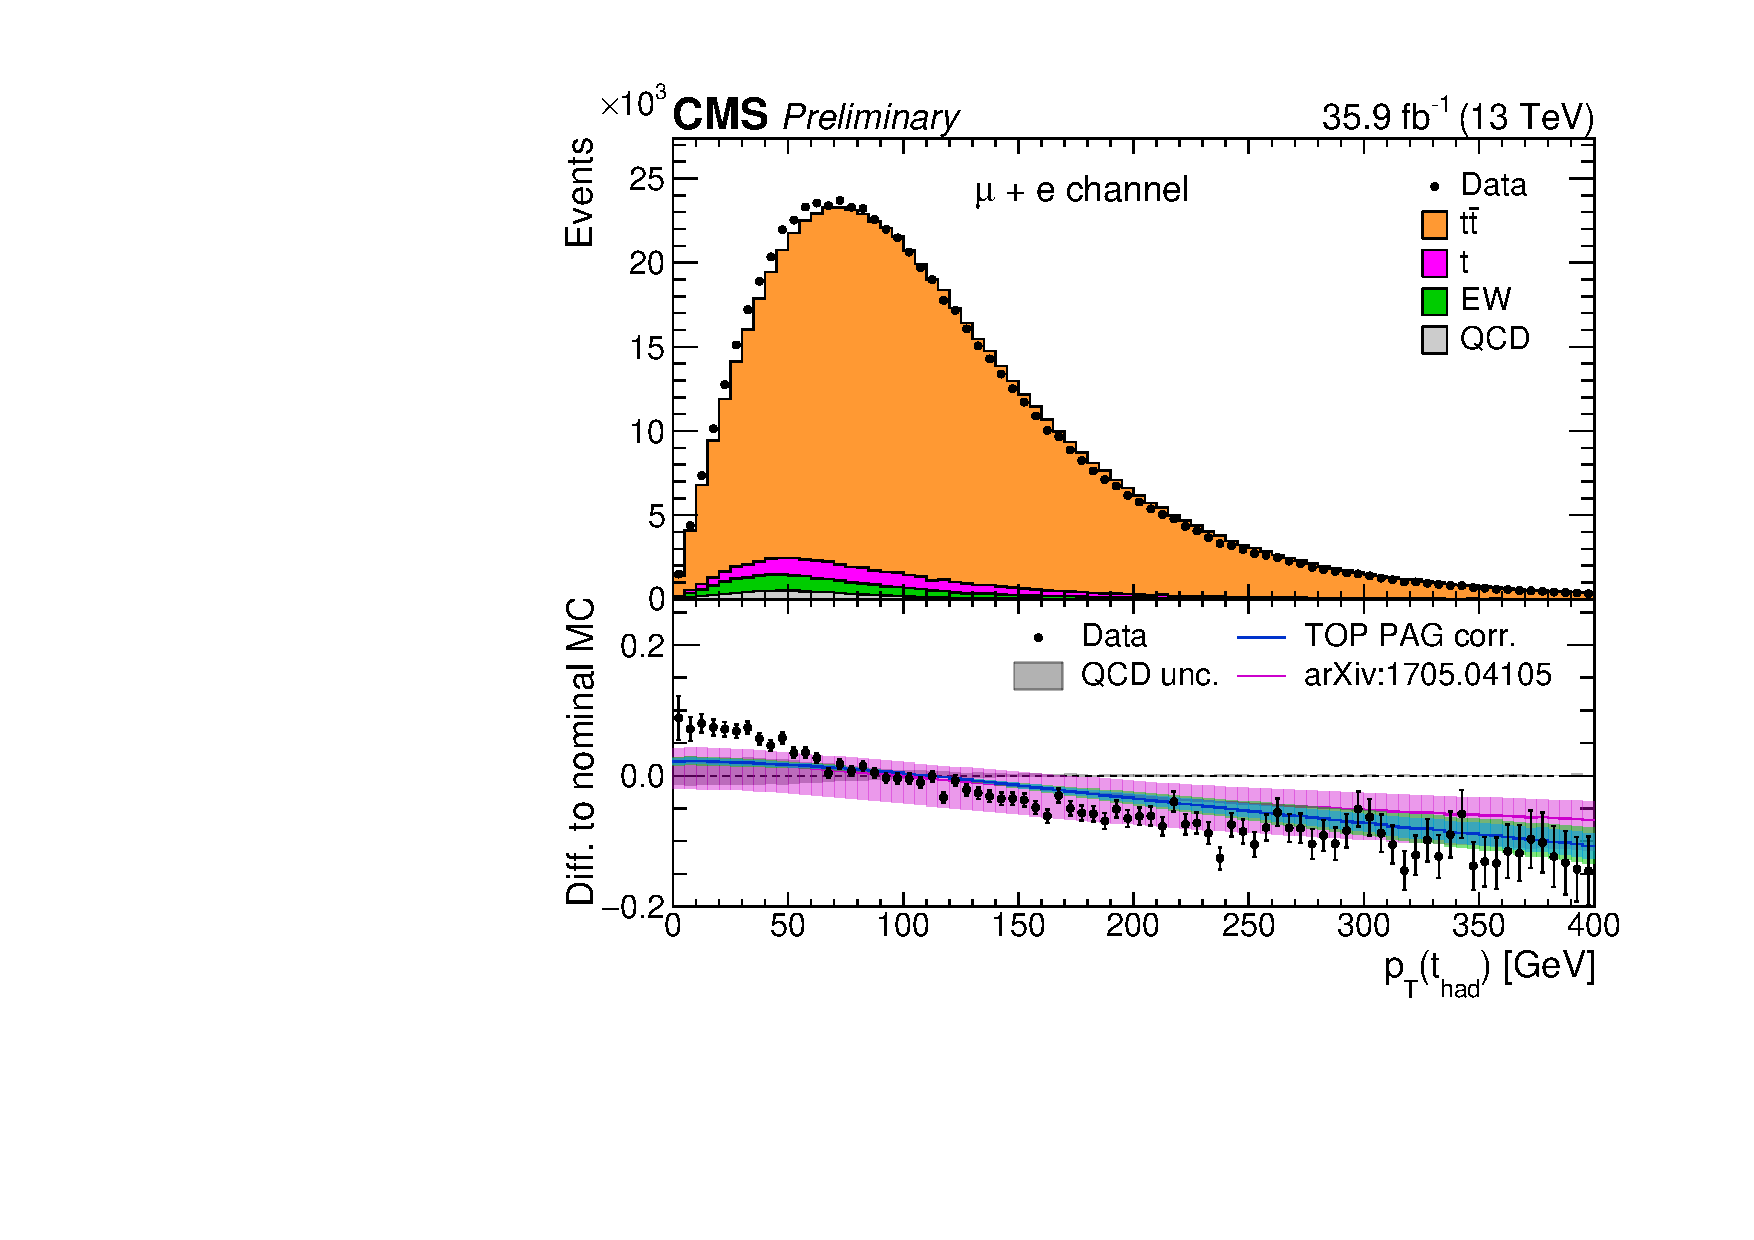
\includegraphics[width=0.45\textwidth]{fig/chapt7/correction/PtTopHad.pdf} \\
  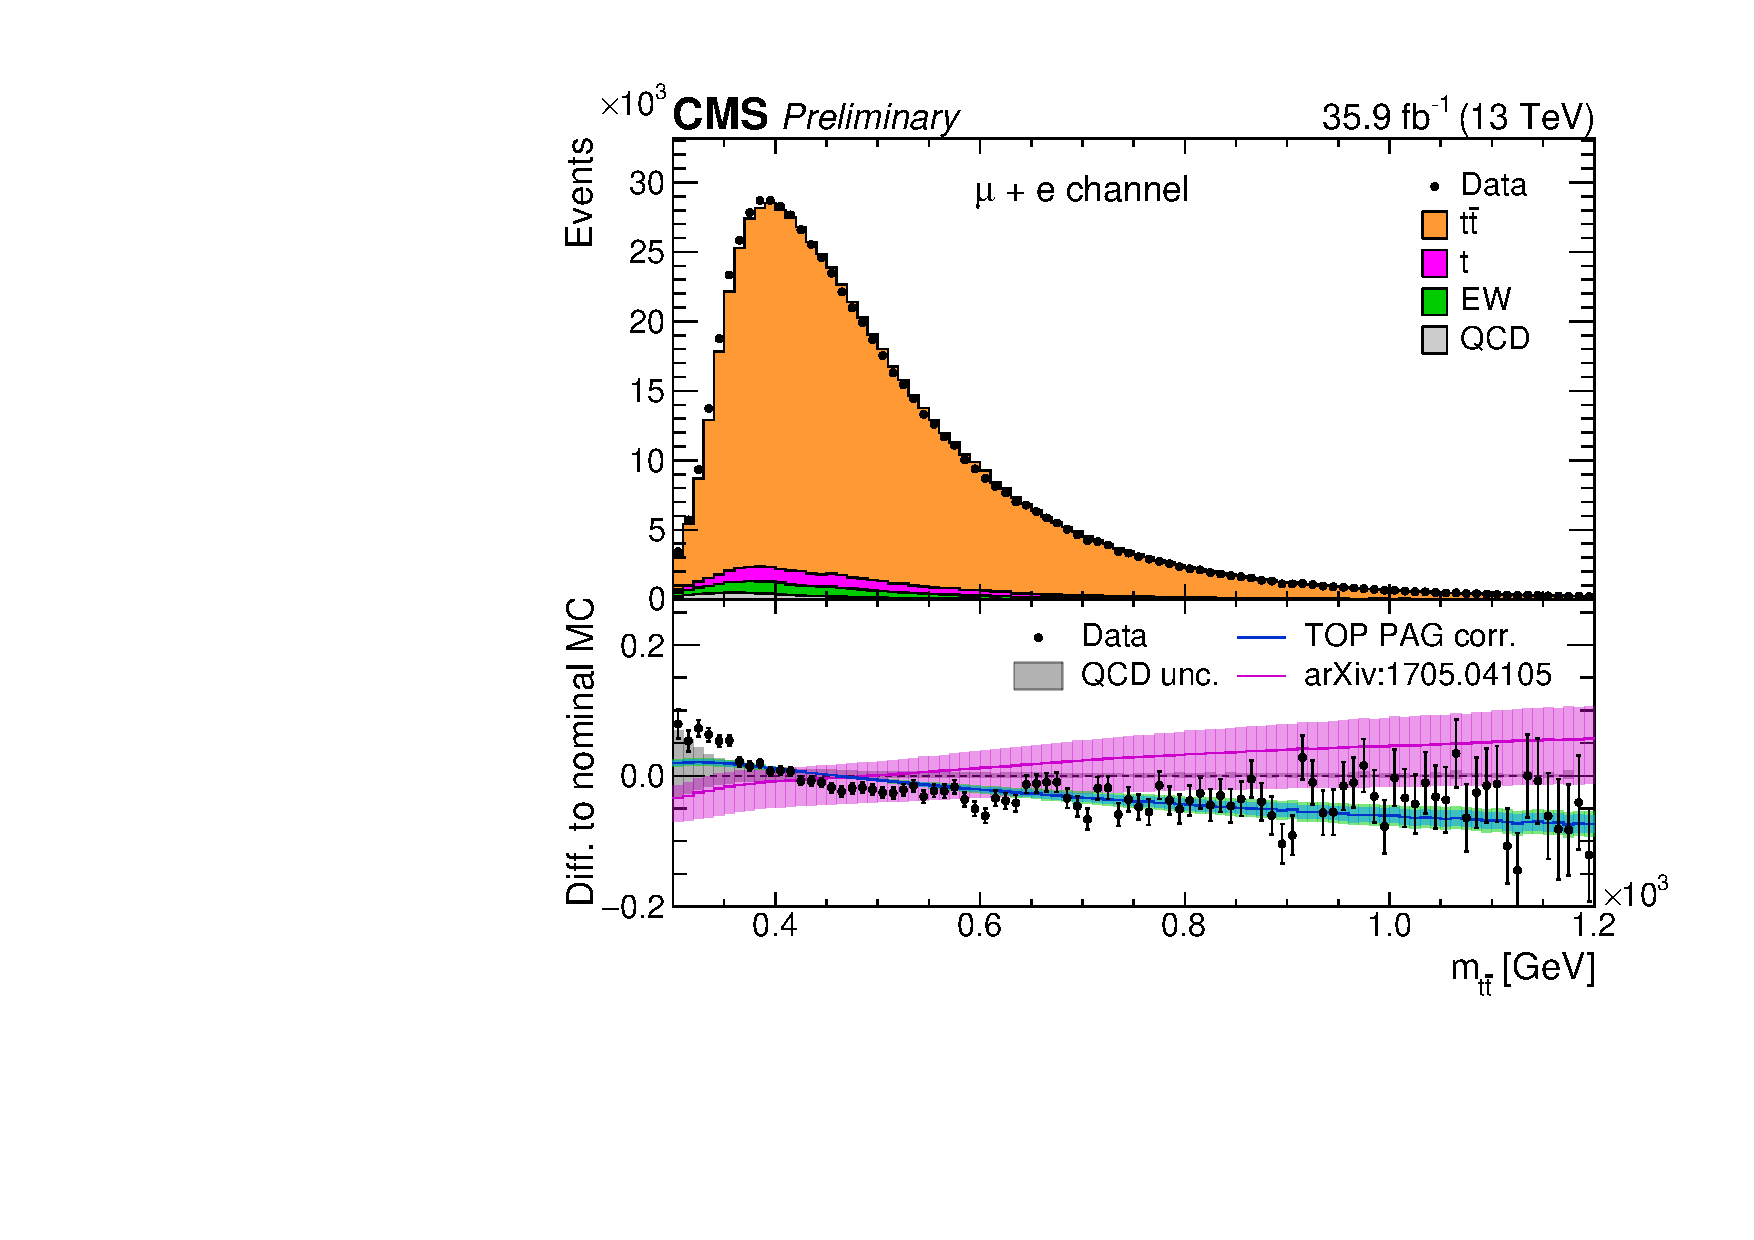
\includegraphics[width=0.45\textwidth]{fig/chapt7/correction/MassTT.pdf}
  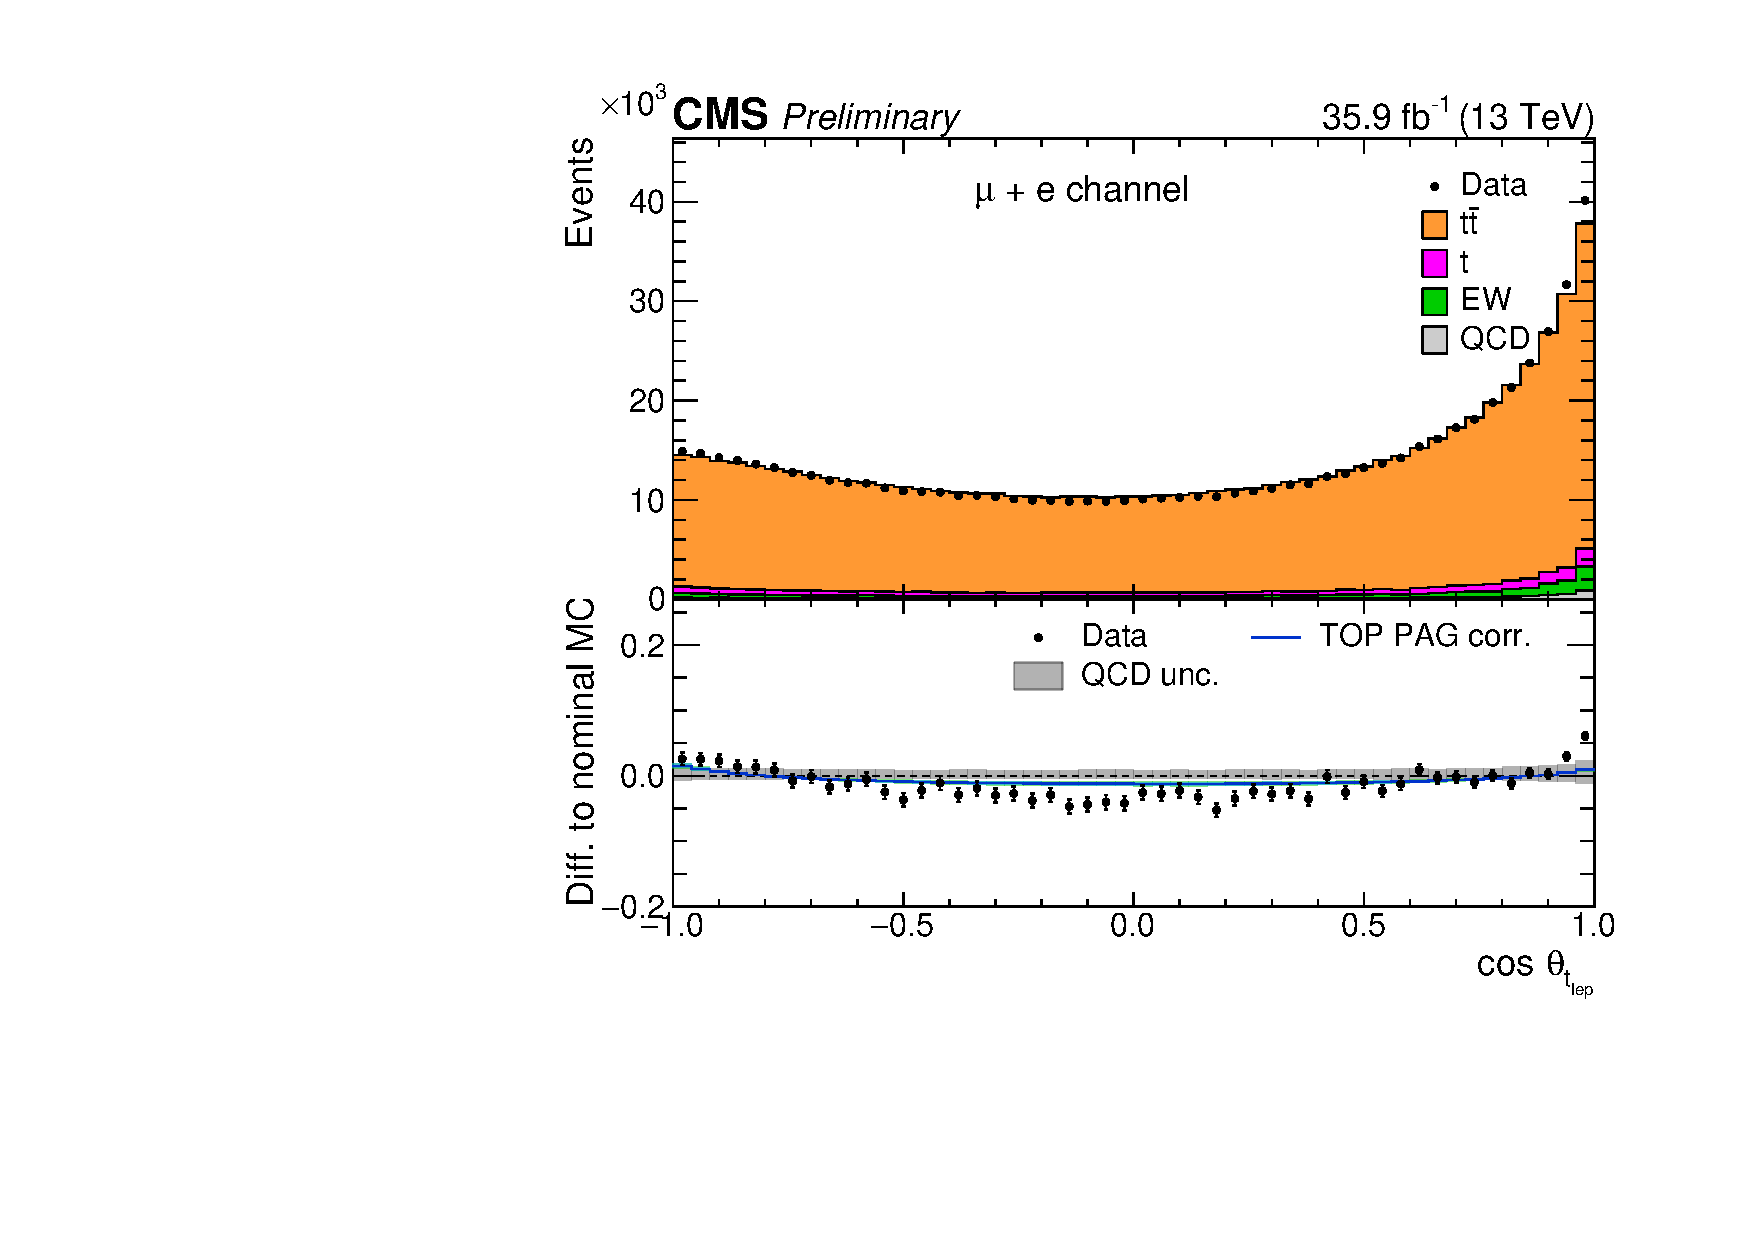
\includegraphics[width=0.45\textwidth]{fig/chapt7/correction/CosTopLepTT.pdf}
  \caption{Effect of the reweighting of SM~$t\bar t$. Shown for $p_{T}$ of the semileptonically and hadronically decaying top quarks (upper row), mass of the $t\bar t$~system (lower left figure), and the angular observable $\cos\theta^{\star}_{t_{l}}$ (lower right figure). Simulation of $t\bar t$~production in the stacked plots in the upper parts of the figures does not have the reweighting applied. The lower parts show relative differences from the full expectation without the $t\bar t$~reweighting. The empirical reweighting discussed in the text is shown with (largely overlapping) blue and green bands, which correspond to the two systematic variations. For comparison, also included are the results of reweighting to differential distributions in Ref.~\cite{Czakon:2017wor}, which are available for top~$p_{T}$ and $m_{t\bar t}$ (magenta bands). The grey bands show the effect of ${+100} / {-50}$\% variation of the normalization of the data-driven multijet background.}
  \label{Fig:TopPtReweighting}
\end{figure}
It should be noted that if the mismodelling of top quark's~$p_{T}$ is caused by unknown BSM effects, the empirical reweighting would hide them from the analysis.
However, these are not the kind of BSM effects that are targeted by this search.
Indeed, the sought-for signal would manifest itself with a peak--dip structure in the $m_{t\bar t}$~spectrum (including the peak-only and dip-only cases as extremes), while the reweighting implements mostly a change of the slope of the data-to-expectation ratio.
As such, it cannot introduce nor absorb features in the $m_{t\bar t}$~distribution.
Corrections to top $p_{T}$ based on pure theoretical values and its uncertainties given in Ref.~\cite{Czakon:2017wor} are also plotted in Fig.~\ref{fig:top_pt_correc_expec}. In Fig.~\ref{fig:top_pt_correc_expec} the leptonic top $p_{T}$ is plotted and in lower pad, a: the PDF uncertainty band and b: the $\mu_{F,R}$ variation from 0 to $\pm$2 are shown. The band shows normalization effect and doesn't cover the whole space which is the reason for using an alternative method from data as described above.  
\begin{figure}[htp]
\centering
\begin{tabular}{cc}
\hspace{-0.5cm}
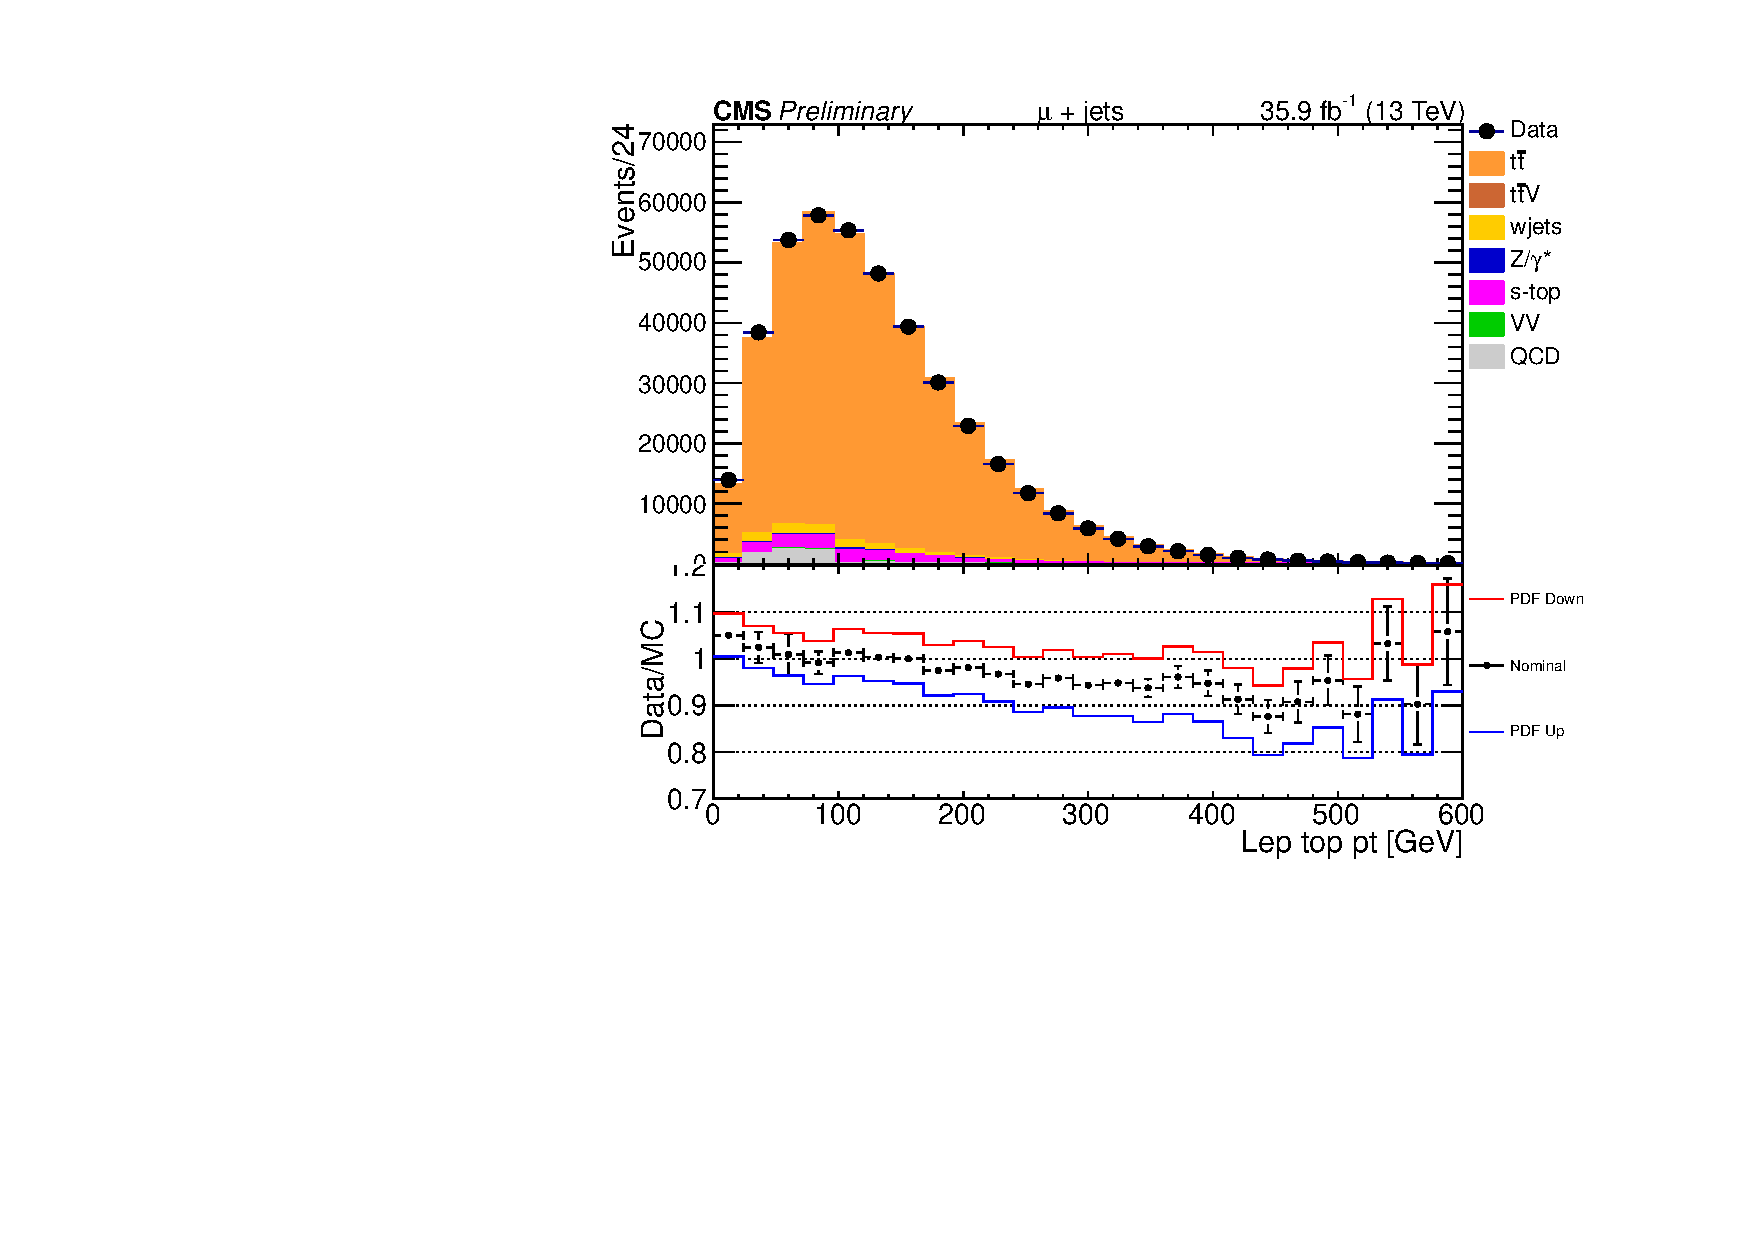
\includegraphics[scale=0.45]{fig/chapt7/correction/lep_topPT_pdf.pdf}
& \hspace{-1.50cm} 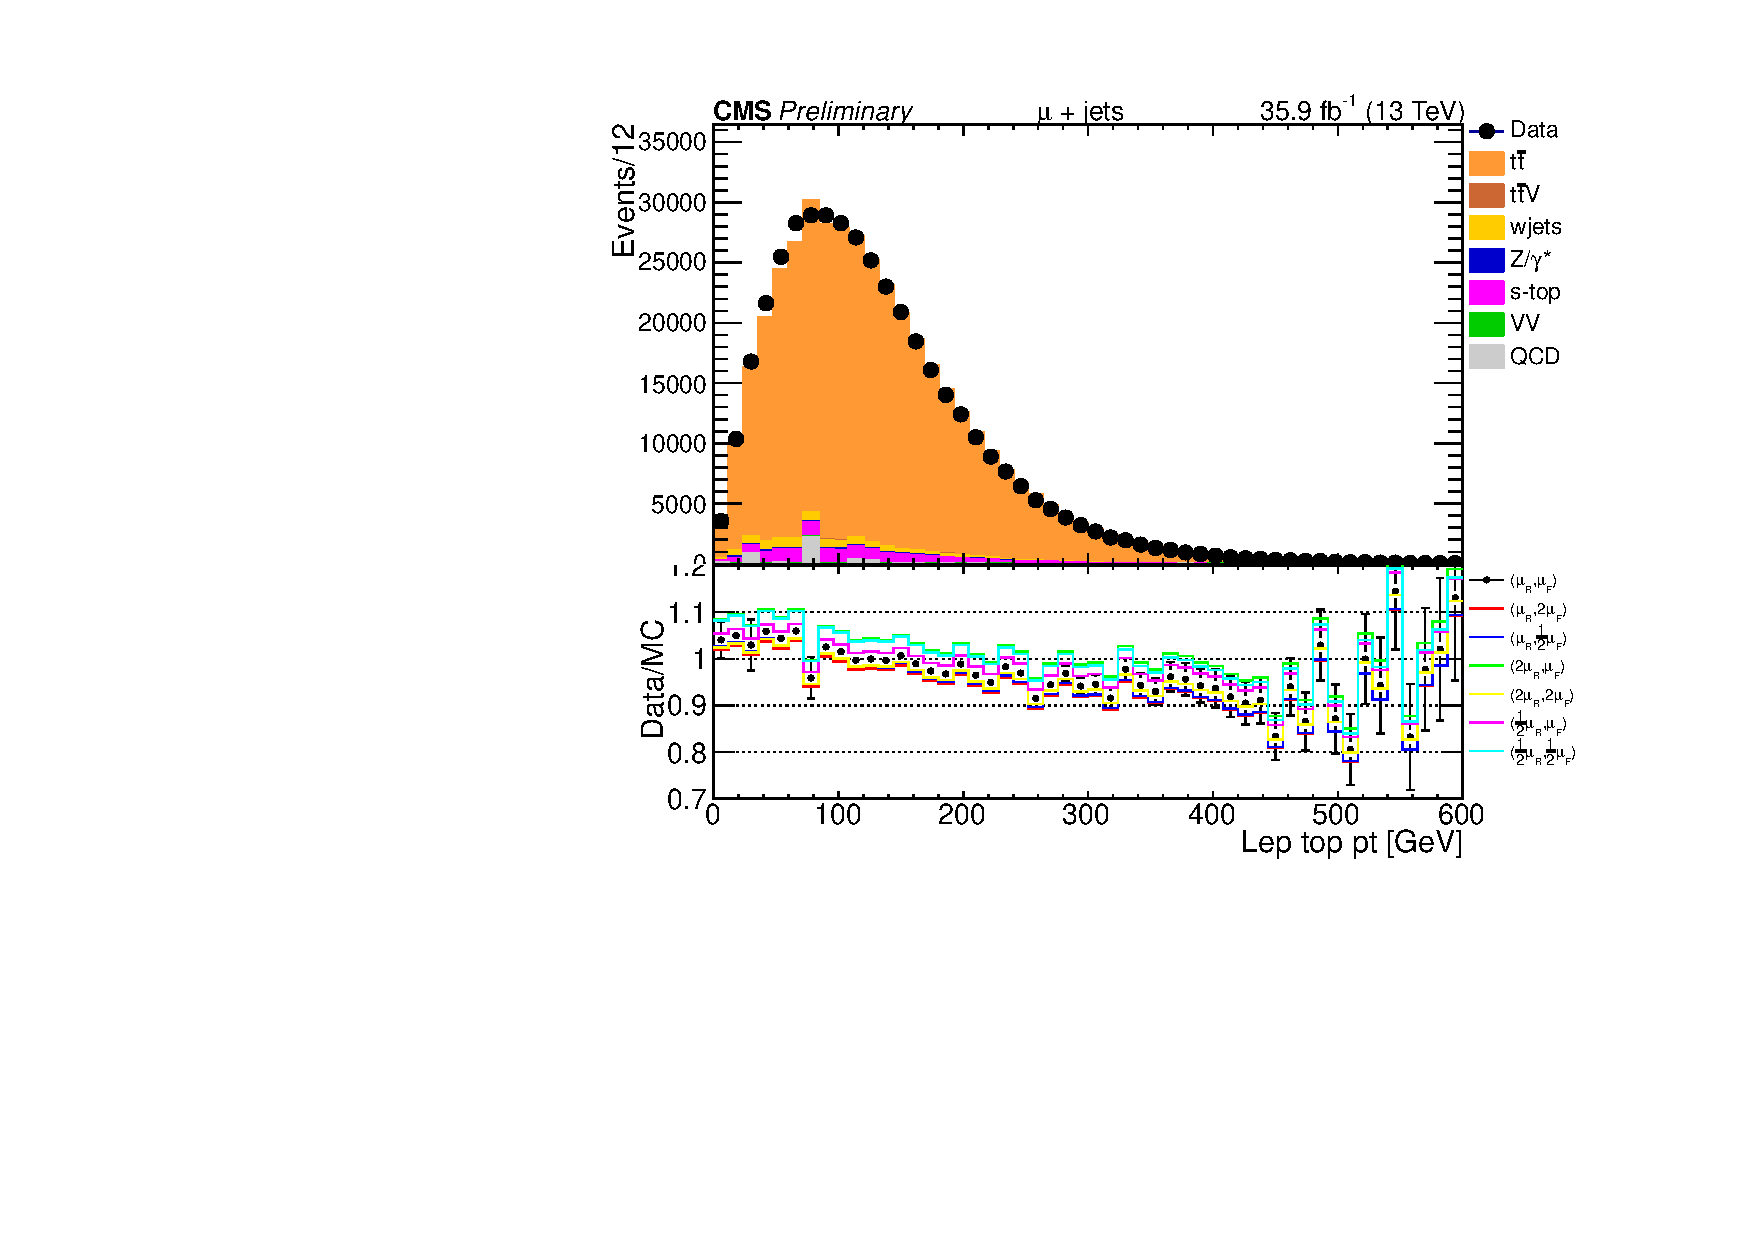
\includegraphics[scale=0.45]{fig/chapt7/correction/lep_top_ren_fac.pdf}\\
  \qquad ($\mathbf{a}$)\qquad\qquad&($\mathbf{b}$)\qquad\qquad\qquad\qquad \\
\end{tabular}
\caption{Corrections from theory to the leptonic top quark $p_{T}$, lower pad a: PDF uncertainty band and b: the $\mu_{F,R}$ variation from 0 to $\pm$2}\label{fig:top_pt_correc_expec}
\end{figure}  


\section{Physics objects selection}\label{Sec:Reconstruction}
For physics objects selection, we require first primary vertex (the one with the greatest sum of $p_{T}^{2}$ of associated physics objects) to be reconstructed in each event from at least four tracks and must not marked as “fake” by the reconstruction algorithm. It should also to lie within a cylinder of radius 2~cm around the nominal beam axis, and its z coordinate must satisfy $\abs{z} <$ 24~cm, where z = 0~cm corresponds to the geometric centre of the CMS detector.\\
Vertices that satisfy the above requirements are exploited to mitigate the impact from additional $pp$ interactions within the same bunch crossing (the pile-up) according to the so-called Charged Hadron Subtraction (CHS) scheme. If a PF candidate is identified as a charged hadron and it is associated to any but the first vertex, the candidate is removed from the event.

\subsubsection*{Muons}\label{sebsec:muon_selection}
%
The analysis uses a PF~candidate which is reconstructed outside-in as a Global Muon satisfying the tight working point of the identification algorithm~\cite{Wiki:MuonID} 
The conditions for this selection requires a goodness-of-fit of its track with $\chi^2/\text{n.\,d.\,f.} < 10$ and at least one muon chamber hit included in the global-muon track fit.
Muon segments in at least two muon stations must be associated with the candidate.
The tracker track's transverse impact parameter with respect to the first primary vertex must satisfy $|d_{xy}| < 2$\,mm, and the $z$~position of the muon vertex must lie within 5\,mm around the $z$~position of the primary vertex.
At least one hit in the pixel system and at least six tracker layers with measurements are required.

In addition to the above identification criteria, the muon must have $p_{T} > 26$\,GeV and $|\eta| < 2.4$ and must be isolated satisfying $I_{\Delta\beta} < 0.15$, where the relative $\Delta\beta$-corrected isolation is defined as
\begin{linenomath}
\begin{equation}
 \label{Eq:IsolationDeltaBeta}
 I_{\Delta\beta} = \frac{1}{p_{T}} \Big(\mathcal I_{h^\pm} + \max\big(\mathcal I_{h^0} + \mathcal I_\gamma - 0.5\cdot \mathcal I_{h^\pm}^\text{PU},\; 0\big)\!\Big).
\end{equation}
\end{linenomath}
Here, values~$\mathcal I$ in the numerator are sums of the transverse momenta of charged hadron, neutral hadron, and photon PF~candidates as well as charged hadron pile-up PF~candidates inside a cone of size $\Delta R = \sqrt{\Delta\eta^2 + \Delta\phi^2} = 0.4$ around the muon, and $p_{T}$ is the transverse momentum of the muon. In $\mathcal I_{h^\pm}^\text{PU}$ term, the contribution of neutral particles from pile-up interactions has been subtracted; the specific form of this correction can be either based on the PF~algorithm ($\Delta\beta$-correction) or on the average energy density measured in the event (effective-area correction).
The kinematic selection is driven by exploited triggers, while isolation is defined as recommended in Ref.~\cite{Wiki:MuonID}.

A muon satisfying the above requirements is referred to as a ``tight'' muon.
For the purpose of event selection, ``loose'' muons are also defined.
They are required to pass the loose working point of the identification algorithm~\cite{Wiki:MuonID}, which is to be muon PF~candidates that are at the same time global or tracker muons, and to satisfy $p_{T} > 10$~GeV, $\abs{\eta} < 2.5$, and $I_{\Delta\beta} < 0.25$.

\subsection*{Electron}\label{subsec:electron}

Similarly to the case of muons, ``tight'' and ``loose'' electrons are exploited.
They are defined according to the tight and the veto working points of the 2016 identification algorithm, respectively.
In case of ``tight'' electrons also the recommended selection on transverse and longitudinal impact parameters, namely $|d_{xy}| < 0.5$ (1)~mm and $|d_z| < 1$ (2)~mm in the ECAL barrel (endcaps), is applied.

In addition, a ``tight'' electron must have $p_{T} > 30$~GeV and $|\eta_\text{SC}| < 2.5$, excluding the transition region between the barrel and the endcap of the ECAL, $1.4442 < |\eta_\text{SC}| < 1.5660$, where $\eta_\text{SC}$ is the pseudorapidity of the associated ECAL supercluster, computed with respect to the geometrical centre of the CMS detector.

``Loose'' electrons are only required to have $p_{T} > 20$~GeV and $|\eta_\text{SC}| < 2.5$ in addition to the criteria of the identification algorithm.

\subsection*{Jets}\label{subsec:jets}
Jets are clustered using the anti-$k_{T}$ algorithm~\cite{Cacciari:2008gp} with a cone size of 0.4.
Pile-up charged hadrons are removed from the source collection for clustering, as described above.
Reconstructed jets must satisfy the loose working point of the PF~jet identification algorithm~\cite{Wiki:JetID}, which applies selection on the number of charged and neutral PF~candidates clustered in the jet and fractions of the total energy carried by different types of constituent PF~candidates.

In order to account for non-linearity of the calorimeter response, impact of minimum energy thresholds, and non-perfect modelling of the detector, several corrections are applied to measured jet momenta~\cite{Khachatryan:2016kdb, CMS-DP-2016-020}.
First, contribution to jet energy from pile-up is subtracted (on the average) using the L1FastJet corrections.
Then the L2L3 corrections are applied in both data and simulation.
They are derived in simulation and correct jet momentum to match transverse momentum of the corresponding particle-level jet.
Finally, jets in data are subject to the L2L3Residual corrections, which account for mismodelling of the detector response.
The version of jet energy corrections (JEC) used in this search is \texttt{Summer16\char`_23Sep2016ReReco\char`_V4}.

Jet energy resolution (JER) in data is known to be worse than predicted by simulation~\cite{Khachatryan:2016kdb}.
In order to account for this difference, jets in simulation are smeared following the recommended ``hybrid'' approach~\cite{Wiki:JetResolution}.
Namely, momenta of reconstructed jets that have matching particle-level jets are scaled with factors
\begin{linenomath}
\begin{equation}
 c_\text{JER} = 1 + (s_\text{JER} - 1)\,\frac{p_{T} - p_{T}^\text{ptcl}}{p_{T}},
 \label{Eq:JER1}
\end{equation}
\end{linenomath}
where $p_{T}$ and $p_{T}^\text{ptcl}$ are transverse momenta of the reconstructed jet and the corresponding particle-level jet, and $s_\text{JER}$ is the JER scale factor provided in Refs.~\cite{Wiki:JetResolution, CMS-AN-16-351}.
The matching particle-level jet is required to satisfy $\Delta R = \sqrt{\Delta\eta^2 + \Delta\phi^2} < 0.2$, which is the half of the jet cone size, and $|p_{T} - p_{T}^\text{ptcl}| < 3\,\sigma_\text{JER}\,p_{T}$, where $\sigma_\text{JER}$ is the relative $p_{T}$~resolution determined from simulation~\cite{CMS-AN-16-116}.
In rare cases when no particle-level jet is matched, jet momentum is rescaled using a stochastic factor
\begin{linenomath}
\begin{equation}
 c_\text{JER} = 1 + \mathcal N(0, \sigma_\text{JER}^2)\,\sqrt{\max(s_\text{JER}^2 - 1, 0)},
 \label{Eq:JER2}
\end{equation}
\end{linenomath}
where $\mathcal N(0, \sigma^2)$ denotes a random number sampled from a normal distribution with a zero mean and variance~$\sigma^2$.
Jet energy resolution and scale factors of version \texttt{Spring16\char`_25nsV10} are utilized.

Jets with $p_{T} > 20$\,~GeV{} and $|\eta| < 2.4$ are considered in this analysis.
Since jets are clustered from all non-pile-up PF~candidates, leptons defined as described above can also be reconstructed as jets.
To prevent the double counting, jets overlapping with a ``loose'' muon or electron within $\Delta R < 0.4$ are removed from the event.

As the signal signature involves b~quarks, the b-tagging capability of the detector is exploited in the analysis.
Jets produced by b~quarks are identified with the help of the updated combined MVA (cMVAv2) algorithm~\cite{CMS-PAS-BTV-15-001}, which combines several individual algorithms.
Indirectly, it makes use of impact parameters of individual tracks in the jet, properties of reconstructed secondary vertices and also soft muons and electrons originating from decays of B~hadrons, and other observables.
The medium working point of the algorithm is utilized, which corresponds to the b-tagging discriminator value larger than 0.4432.
Selection efficiency for b~quark (light-flavour) jets is about 65\% (1\%).

\subsubsection*{Missing transverse momentum}\label{subsec:met}
%
Reconstruction of neutrino from the decay $t \rightarrow bl\nu$ exploits missing transverse momentum
\begin{linenomath}
\begin{equation}
\vv{p}_{T}^{miss} = -\sum_i \vv{p}_{T}(i) - \sum_j \left(\vv{p}_{T}(j) - \vv{p}_{T}^\text{\,L1}(j)\right).
\end{equation}
\end{linenomath}
The first sum runs over all PF~candidates, including those that have been identified by the CHS procedure.
The second sum represents the so-called type-1 correction~\cite{CMS-PAS-JME-16-004} implemented following the $\text{L1L2L3} - \text{L1FastJet}$ scheme.
Here $\vv{p}_{T}(j)$ is the fully corrected transverse momentum of jet~$j$ whereas $\vv{p}_{T}^\text{\,L1}(j)$ denotes its momentum with only the L1FastJet correction applied, and the sum includes all jets with $p_{T} > 15$~GeV that do not overlap with ``loose'' muons or electrons.
JER smearing is not applied in this computation.

Two additional corrections are applied to $p_{T}^{miss}$ in data but not in simulation.
A significant fraction of the 2016 data set was affected by the dynamic tracker inefficiency~\cite{Talk:DTI}.
Its impact was mitigated in reconstruction, but as a side effect duplicate and fake muons were created in some events.
These spurious muons are propagated into $p_{T}^{miss}$ and can thus produce an artificial tail at large values of $p_{T}^{miss}$~\cite{Talk:SpuriousMuons}.
To correct for this bias, duplicate and fake muons are identified with dedicated filters~\cite{HN:GiovanniFilters} and removed from the collection of PF~candidates that is used to compute $p_{T}^{miss}$.
This is done centrally when MiniAOD data are produced~\cite{Talk:FebReMiniAOD}.
The second correction addresses a mismeasurement of ECAL energy deposition for high-$p_{T}$ electrons and photons due to the so-called ECAL gain switch effect~\cite{Talk:ECALGainSwitch}.
The correction that is applied to momenta of electrons and photons, is also propagated into $p_{T}^{miss}$.

\section{Event selection}
\label{Sec:EventSelection}
%
This search targets semileptonic decays $\Phi \rightarrow t\bar t \rightarrow l\,2b\,2q$, where $l$ denotes a muon or an electron.
Decays involving a $\tau$~lepton are not considered explicitly.
Final states with a muon or an electron are referred to as the muon and electron channels respectively.

In the muon channel the analysis is performed with data collected using an inclusive~\textit{or} of triggers \texttt{HLT\_Is-} \texttt{oMu24\_v*} and \texttt{HLT\_IsoTkMu24\_v*}, while in the electron channel trigger \texttt{HLT\_Ele27\_WPTight\_Gsf-} \texttt{\_v*} is exploited.
These triggers were unprescaled throughout 2016 data taking.
Simulated events are subjected to an emulation of the same triggers.

After the trigger selection, an event in the muon (electron) channel is required to contain exactly one ``tight'' muon (electron), as defined in Sec.~\ref{Sec:Reconstruction}.
In order to suppress the contribution from Drell--Yan and other processes in which multiple prompt leptons are produced, an event is rejected if an additional ``loose'' muon or electron is found, regardless of the channel.

Since decay products of the heavy Higgs boson include two b~quarks and two ligher quarks, an event must contain at least four jets, and at least two of them are required to be b-tagged.
The jets are defined as described in Sec.~\ref{Sec:Reconstruction}.
The relatively low $p_{T}$~threshold of 20~GeV is motivated by the spectrum of the subleading non-b quark from the hadronically decaying top quark.

To further suppresss the QCD multijet background, only events with $m_\text{T}^W > 50$~GeV are selected.
The variable $m_\text{T}^W$, which has a characteristic distribution in events containing a leptonically decaying W~boson, is defined as
\begin{linenomath}
\begin{equation}
  m_\text{T}^W = \sqrt{2p_{T}^l p_{T}^{miss} (1 - \cos\Delta\phi(\vv{p}_\text{T}^l, \vv{p}_{T}^{miss})),}
  \label{Eq:MtW}
\end{equation}
\end{linenomath}
where $\vv{p}_\text{T}^l$ is the transverse momentum of the only ``tight'' muon or electron in the event.

Finally, dedicated filters are applied to reject events with anomalous noise or problems in reconstruction~\cite{Wiki:METFilters}, as recommended for analyses that exploit $\vv{p}_{T}^{miss}$.
They target interactions between beam halo muons and calorimeters, anomalous noise in HCAL, unknown and unrecoverable energy depositions in some cells of ECAL~\cite{Talk:ECALTPFilter}, large spontaneous signals from specific supercrystals in EE, poorly reconstructed muons.
In addition, an event is rejected if its first primary vertex does not meet quality requirements listed in Sec.~\ref{Sec:Reconstruction}.

\begin{table}
  \centering
  \caption{Summary of the event selection.}
  \label{Tab:EventSelection}
  \begin{tabular}{l}
  \hline
  \hline
  $\mu$ ($e$) with $p_{T} > 26$ (30)~GeV  \\
  no additional loose muons or electrons  \\
  $\geqslant 4$ jets with $p_{T} > 20$~GeV, $|\eta| < 2.4$  \\
  $\geqslant 2$ b-tagged jets  \\
  $m_\text{T}^W > 50$~GeV \\
  \hline
  \hline
  \end{tabular}
\end{table}

The event selection is briefly summarized in Table~\ref{Tab:EventSelection}.
Resulting observed event yields and expectations for background processes and an example signal benchmark are shown in Table~\ref{Tab:EventYields}.
Combined signal acceptance for targeted decays changes from 7 to 10\% approximately, depending on the mass of the heavy Higgs boson.
The acceptance is computed for the resonant production and is defined as the ratio between the expected number of selected events, summed over the muon and electron channels, and the total expected number of produced events with the $e + \text{jets}$ and $\mu + \text{jets}$ final states.

After applying all cuts and corrections, a good data/MC comparison observed in distributions of basic observable, shown in appendix~\ref{app4}. 

\begin{table}
  \centering
  \caption{Observed and expected event yields. Here V denotes a W or a Z~boson. Numbers for backgrounds include only statistical uncertainties and uncertainties assigned for normalization of individual processes that will be described in Sec.~\ref{Sec:Systematics}. The entry for an example signal benchmark is the sum of contributions from the resonant production and the interference for a $\mathcal{CP}$-even state with mass 500\,GeV, relative total width 10\% of mass, and $g_{Att} = 1$. For signal, the statistical uncertainty and the combined theory uncertainty described in Sec.~\ref{Sec:Systematics} are included.}
  \label{Tab:EventYields}
  \renewcommand{\arraystretch}{1.5}  % increase vertical spacing for readability
  \begin{tabular}{lcc}
  \hline
  \hline
  \multicolumn{1}{c}{Process}  & Muon channel  & Electron channel \\
  \hline
  Data              & 483359                                   & 326346  \medskip\\
  $t\bar{t}$        & $\left(435^{+26}_{-25}\right)10^{3}$    & $\left(288 \pm 17\right)10^{3}$  \\
  Single top        & $\left(24^{+3}_{-2}\right)10^{3}$       & $\left(16.1^{+1.9}_{-1.7}\right)10^{3}$  \\
  W                 & $\left(17^{+9}_{-6}\right)10^{3}$       & $\left(11^{+5}_{-4}\right)10^{3}$  \\
  $Z/\gamma^*$      & $\left(2.2^{+1.1}_{-0.7}\right)10^{3}$  & $\left(2.1^{+1.0}_{-0.7}\right)10^{3}$  \\
  VV                & $\left(0.6^{+0.3}_{-0.2}\right)10^{3}$  & $360^{+180}_{-120}$  \\
  $t\bar{t}V$  & $\left(1.2 \pm 0.3\right)10^{3}$        & $810^{+250}_{-190}$  \\
  Multijet          & $\left(7^{+8}_{-4}\right)10^{3}$        & $\left(11^{+12}_{-6}\right)10^{3}$  \medskip\\
  Total background  & $\left(491^{+28}_{-27}\right)10^{3}$    & $\left(332^{+22}_{-19}\right)10^{3}$  \medskip\\
  Signal (A, 500\,GeV, 10\%)  & $-570^{+330}_{-370}$  & $-450^{+240}_{-270}$  \\
  \hline
  \hline
  \end{tabular}
\end{table}

\section{Search variables}
\label{Sec:SearchVars}
%
This section discusses the two search variables exploited in this analysis.
They are defined based on reconstructed top quarks, which approximate the underlying parton-level system.

\subsection{Reconstruction of the $t\bar t$ system}\label{subsec:ttbar_reco}
%
Each event that passes the selection described in the previous section is reconstructed under the assumption that it has been produced in the process $pp \rightarrow t\bar t \rightarrow l\nu\,2b\,2q$.
This is done using a variant of the algorithm adopted in Ref.~\cite{Khachatryan:2016mnb}.
All possible ways to assign four reconstructed jets to the four quarks in the final state are considered.
In order to reduce the number of combinations, it is required that each of the two b~quarks is associated with a b-tagged jet.
Out of the remaining jet assignments, the algorithm chooses the one with the largest value of the likelihood function constructed as described below.

For each considered choice of $b_{l}$, the b~quark jet stemming from the semileptonically decaying top quark, the neutrino is reconstructed following the procedure introduced in Ref.~\cite{Betchart:2013nba}.
The $z$~component of its momentum is not known, and while the transverse component can be approximated by the measured $\vv{p}_{T}^{miss}$, the accuracy of such an approximation is severely limited by the resolution of this observable.
Because of this, the algorithm treats the whole neutrino's three-momentum as unknown.
It is determined by utilizing mass constraints $(p(l) + p(\nu))^2 = m_{W}^2$ and $(p(l) + p(\nu) + p(b_{l}))^2 = m_{t}^2$, which typically result in a one-dimensional space of allowed solutions for $\vv{p}(\nu)$.
A unique solution is then chosen by minimizing the Euclidean distance $D_\nu = |\vv{p}_{T}(\nu) - \vv{p}_{T}^{miss}|$.

\begin{figure}
  \centering
  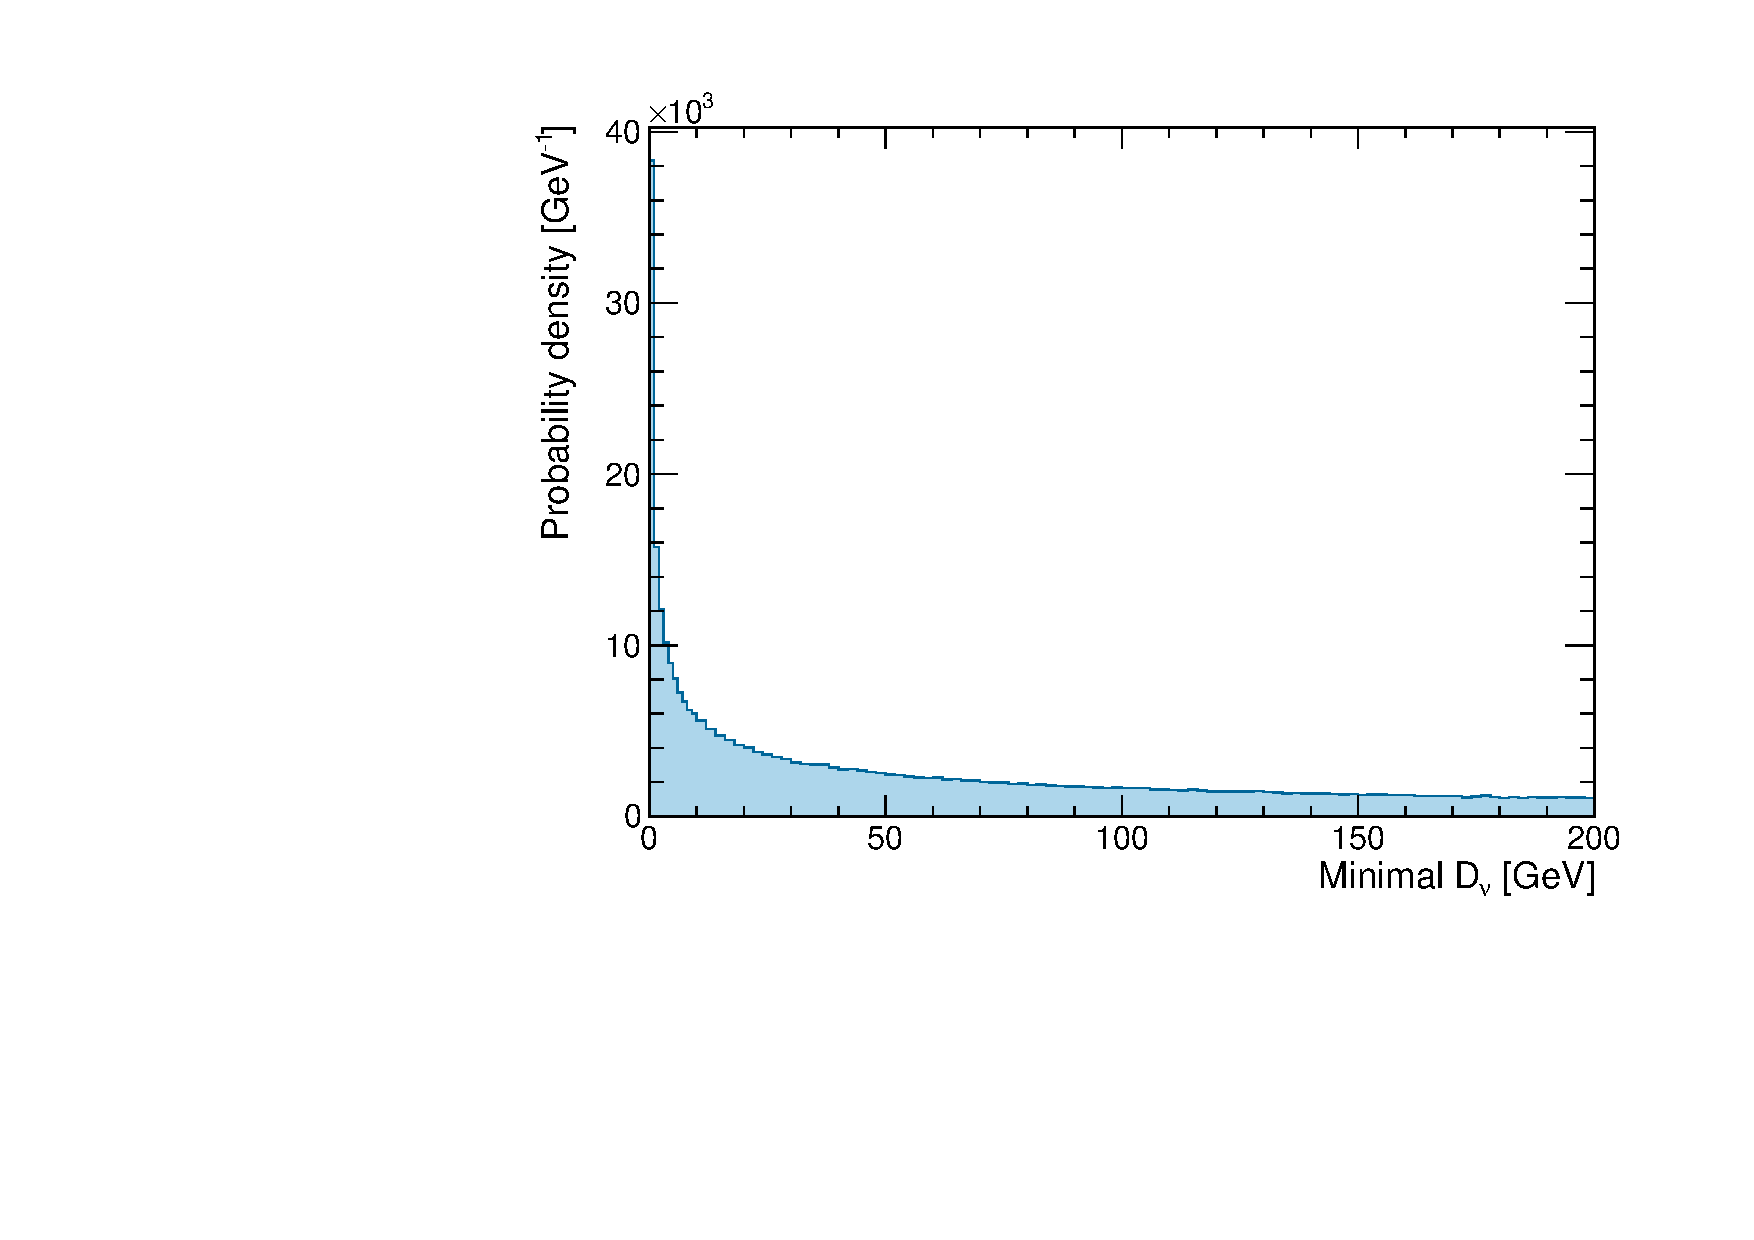
\includegraphics[width=0.45\textwidth]{fig/chapt5/Dnu.pdf}
  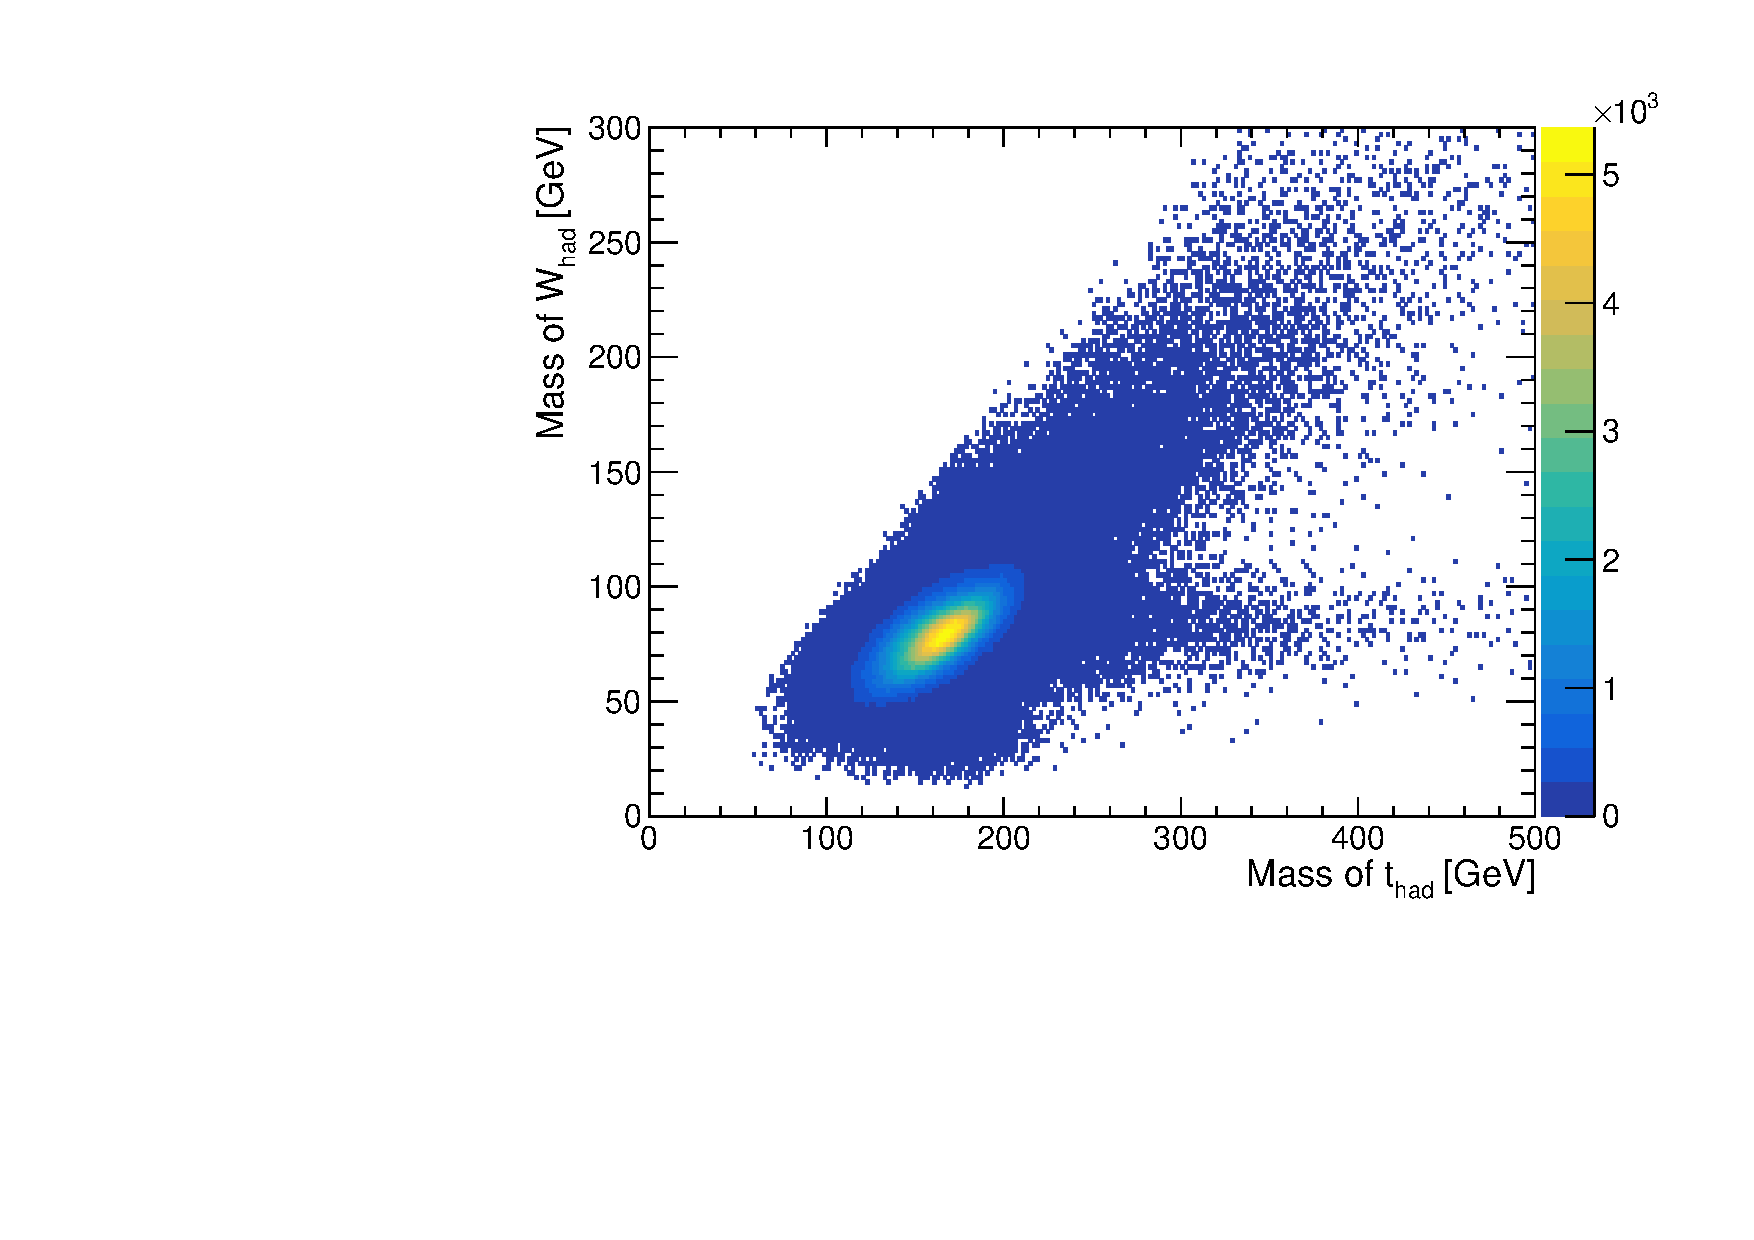
\includegraphics[width=0.45\textwidth]{fig/chapt5/M3.pdf}
  \caption{Components of the likelihood function for $t\bar t$~reconstruction: minimal $D_{\nu}$ (left) and masses involved in the hadronic branch of the decay (right).}
  \label{Fig:TTRecoLikelihood}
\end{figure}

The likelihood function is constructed using $t\bar t$ events with the correct jet assignment, which is performed according to the $\Delta R$ matching between reconstructed jets and generated partons.
In is computed as a product of two components.
The first one is the probability density of the minimal $D_{\nu}$, and the second component is the two-dimensional probability density of reconstructed masses of the top quark and the W~boson in the hadronic branch of the $t\bar t$~decay.
The two probability densities are shown in Fig.~\ref{Fig:TTRecoLikelihood}.
Among all considered jet assignments, the one with the greatest value of $L(D_{\nu}) \cdot L(m_{t}^\text{reco}, m_{W}^\text{reco})$ is selected.
This jet assignment also fixes momentum of the neutrino, which allows reconstructing the semileptonically decaying top quark.

Under some circumstances the $t\bar t$~reconstruction can fail.
The most common reason for the failure is the absence of a solution for neutrino's momentum when $(p(l) + p(b_l))^2 > m_t^2$ for all possible choices of $b_l$.
This might point to a largely mismeasured momentum of the jet or indicate that the actual jet from the decay $t \rightarrow bl\nu$ has not been reconstructed or has not passed the b-tagging requirement.
More rarely, the reconstruction fails if the likelihood is zero for all considered jet assignments.
Events for which the $t\bar t$~reconstruction has not succeeded are excluded from the subsequent analysis.
For SM~$t\bar t$ this amounts to about 12\% of events, some of which originate from other decays than the targeted $l + \text{jets}$ final state.

The performance of the $t\bar t$~reconstruction is studied below using SM~$t\bar t$ events that pass the event selection.
Additionally, only events with the targeted decays are considered, which further rejects about 15\% of events.
Kinematic requirements applied to jets as well as imperfection of the jet reconstruction and b-tagging limit the maximal achievable performance of the jet assignment algorithm, which is illustrated in Fig.~\ref{Fig:TTRecoPartonMatch}.
In the left panel it shows the probability that a quark from the $t\bar t$~decay is matched to a reconstructed jet within $\Delta R < 0.4$.
It can be seen that even with a perfect $t\bar t$~reconstruction it would only be possible to identify all the four jets correctly in about 55\% of cases.
In the remaining events the subleading non-b-quark jet from the decay often does not satisfy the kinematic requirements imposed in this analysis.
The right-hand panel shows that even when both b~quarks can be matched to reconstructed jets, in about 20\% of cases one of these jets does not pass the b-tagging requirement, which can happen, for instance, when one of the two b-tagged jets required by the event selection stems from the hadronization of the c~quark from the $W \rightarrow cs$ decay.
This further reduces the maximal achievable efficiency of the $t\bar t$~reconstruction.
In the following events in which each of the four quarks can be matched to reconstructed jets and the jets matched to the b~quarks are b-tagged are referred to as fully reconstructable events.

\begin{figure}
  \centering
  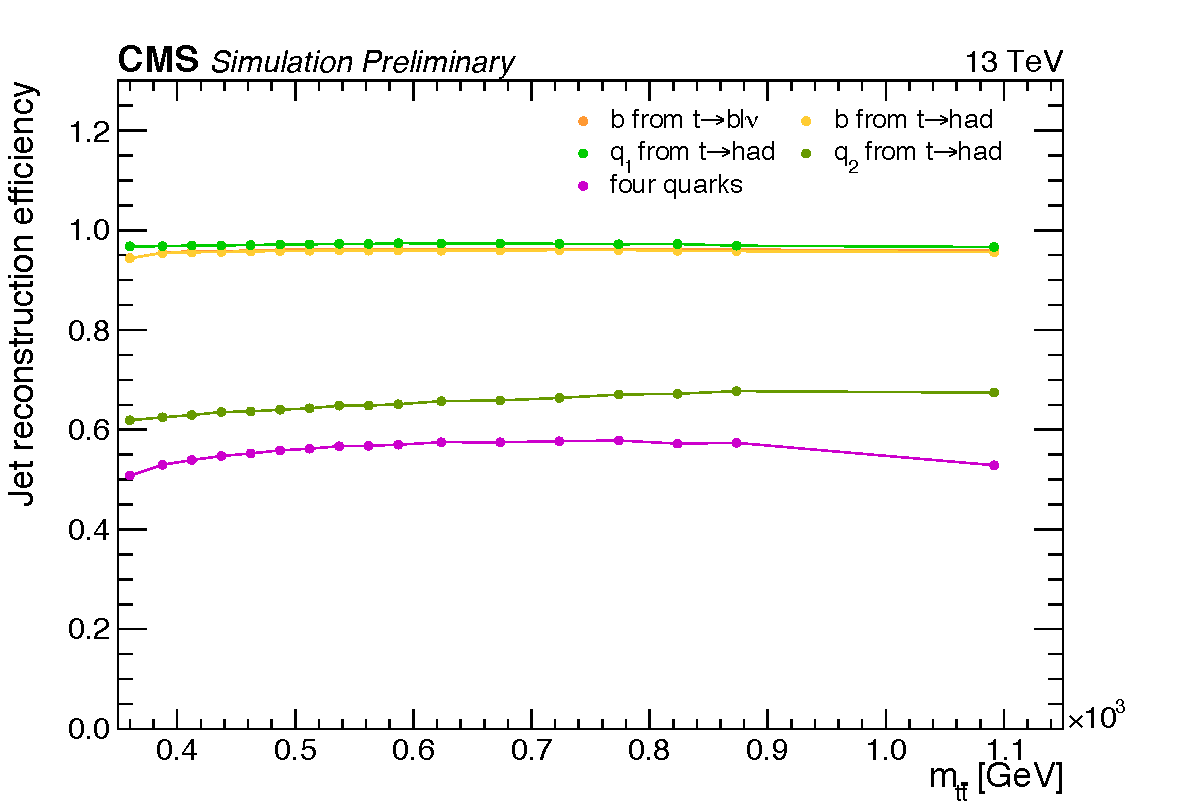
\includegraphics[width=0.45\textwidth]{fig/chapt5/perf/matching.pdf}
  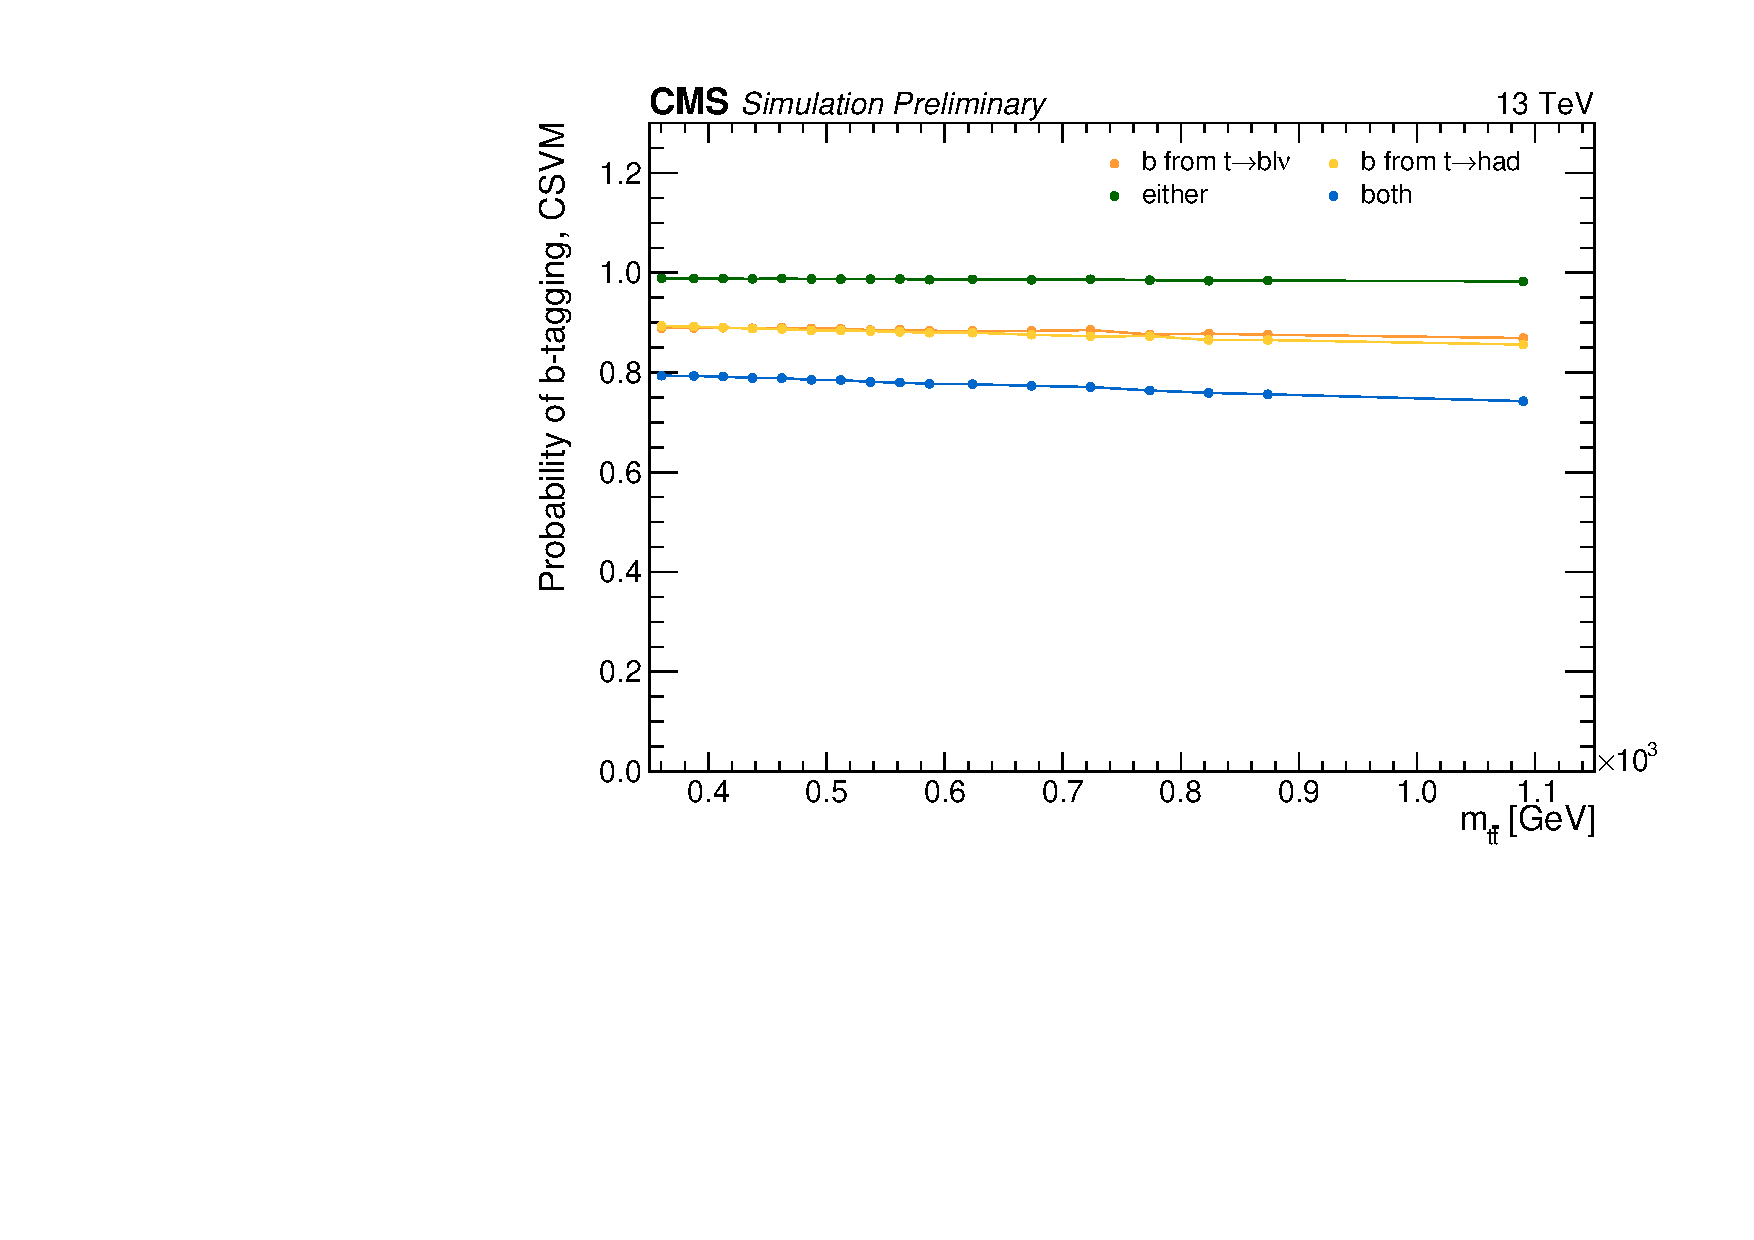
\includegraphics[width=0.45\textwidth]{fig/chapt5/perf/btag.pdf}
  \caption{Efficiency of reconstuction of jets stemming from the four quarks in the final state of the $t\bar t$~decay (left) and the b-tagging probability for jets matched to the two b~quarks (right). Shown as a function of parton-level $m_{t\bar t}$.}
  \label{Fig:TTRecoPartonMatch}
\end{figure}

The performance of the actual $t\bar t$~reconstruction algorithm is quantified over the fully reconstructable events, and the results are provided in Fig.~\ref{Fig:TTRefoEff}.
The algorithm declares the reconstruction successful in more than about 97\% of cases, and these events are used to determine the probability of correct assignment of reconstructed jets to the four quarks in the final state.
The probability that all the four jets are correctly identified varies from 60 to 80\% depending on the value of~$m_{t\bar t}$.
The resolution and the bias of the measured value of~$m_{t\bar t}$ are shown in Fig.~\ref{Fig:TTRecoMttPerf}.
They are computed as the standard deviation and the mean of distribution of $(m_{t\bar t}^\text{reco} - m_{t\bar t}^\text{parton}) / m_{t\bar t}^\text{parton}$ respectively.
The mass resolution is found to be about 14\%.
It should be noted that if not only fully reconstructable events were considered, the apparent resolution would be worse.

\begin{figure}
  \centering
  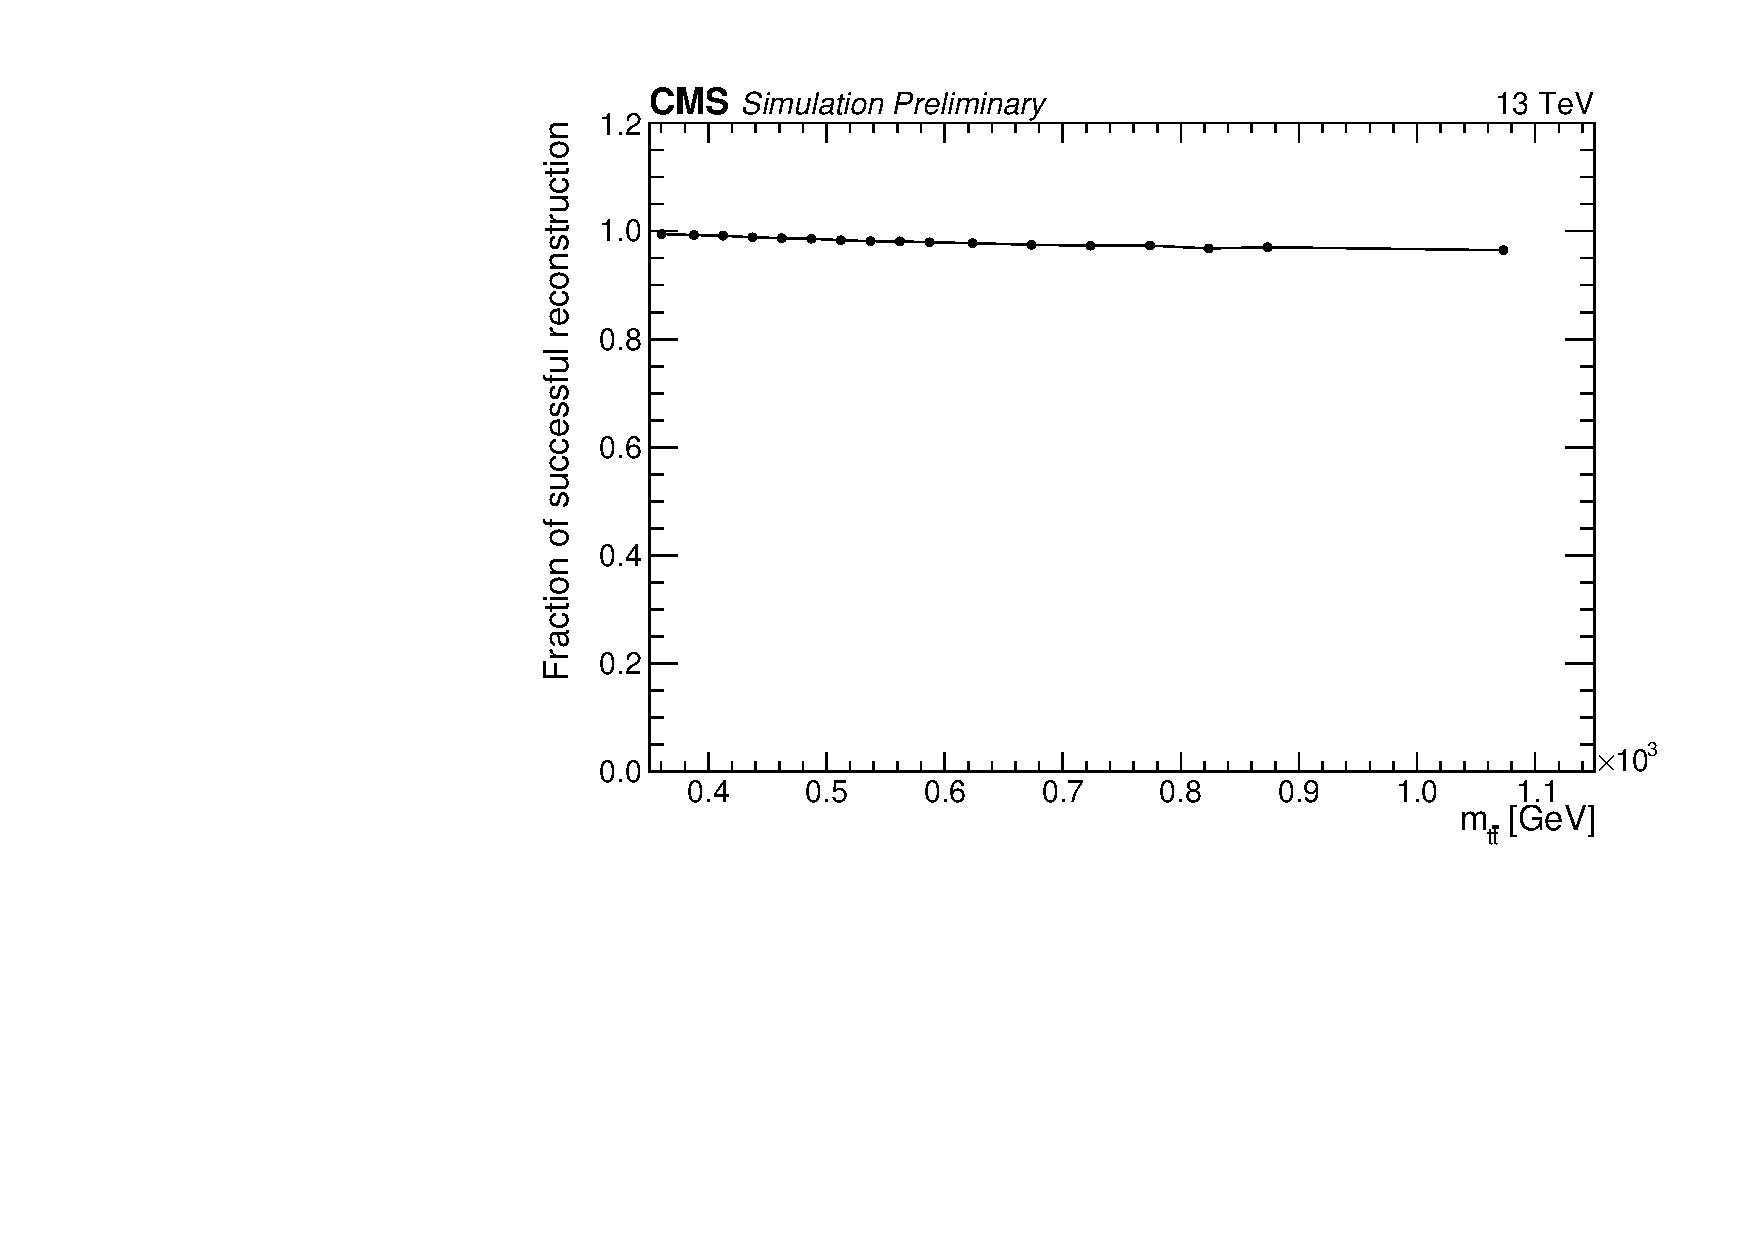
\includegraphics[width=0.45\textwidth]{fig/chapt5/perf/recoSuccess.pdf}
  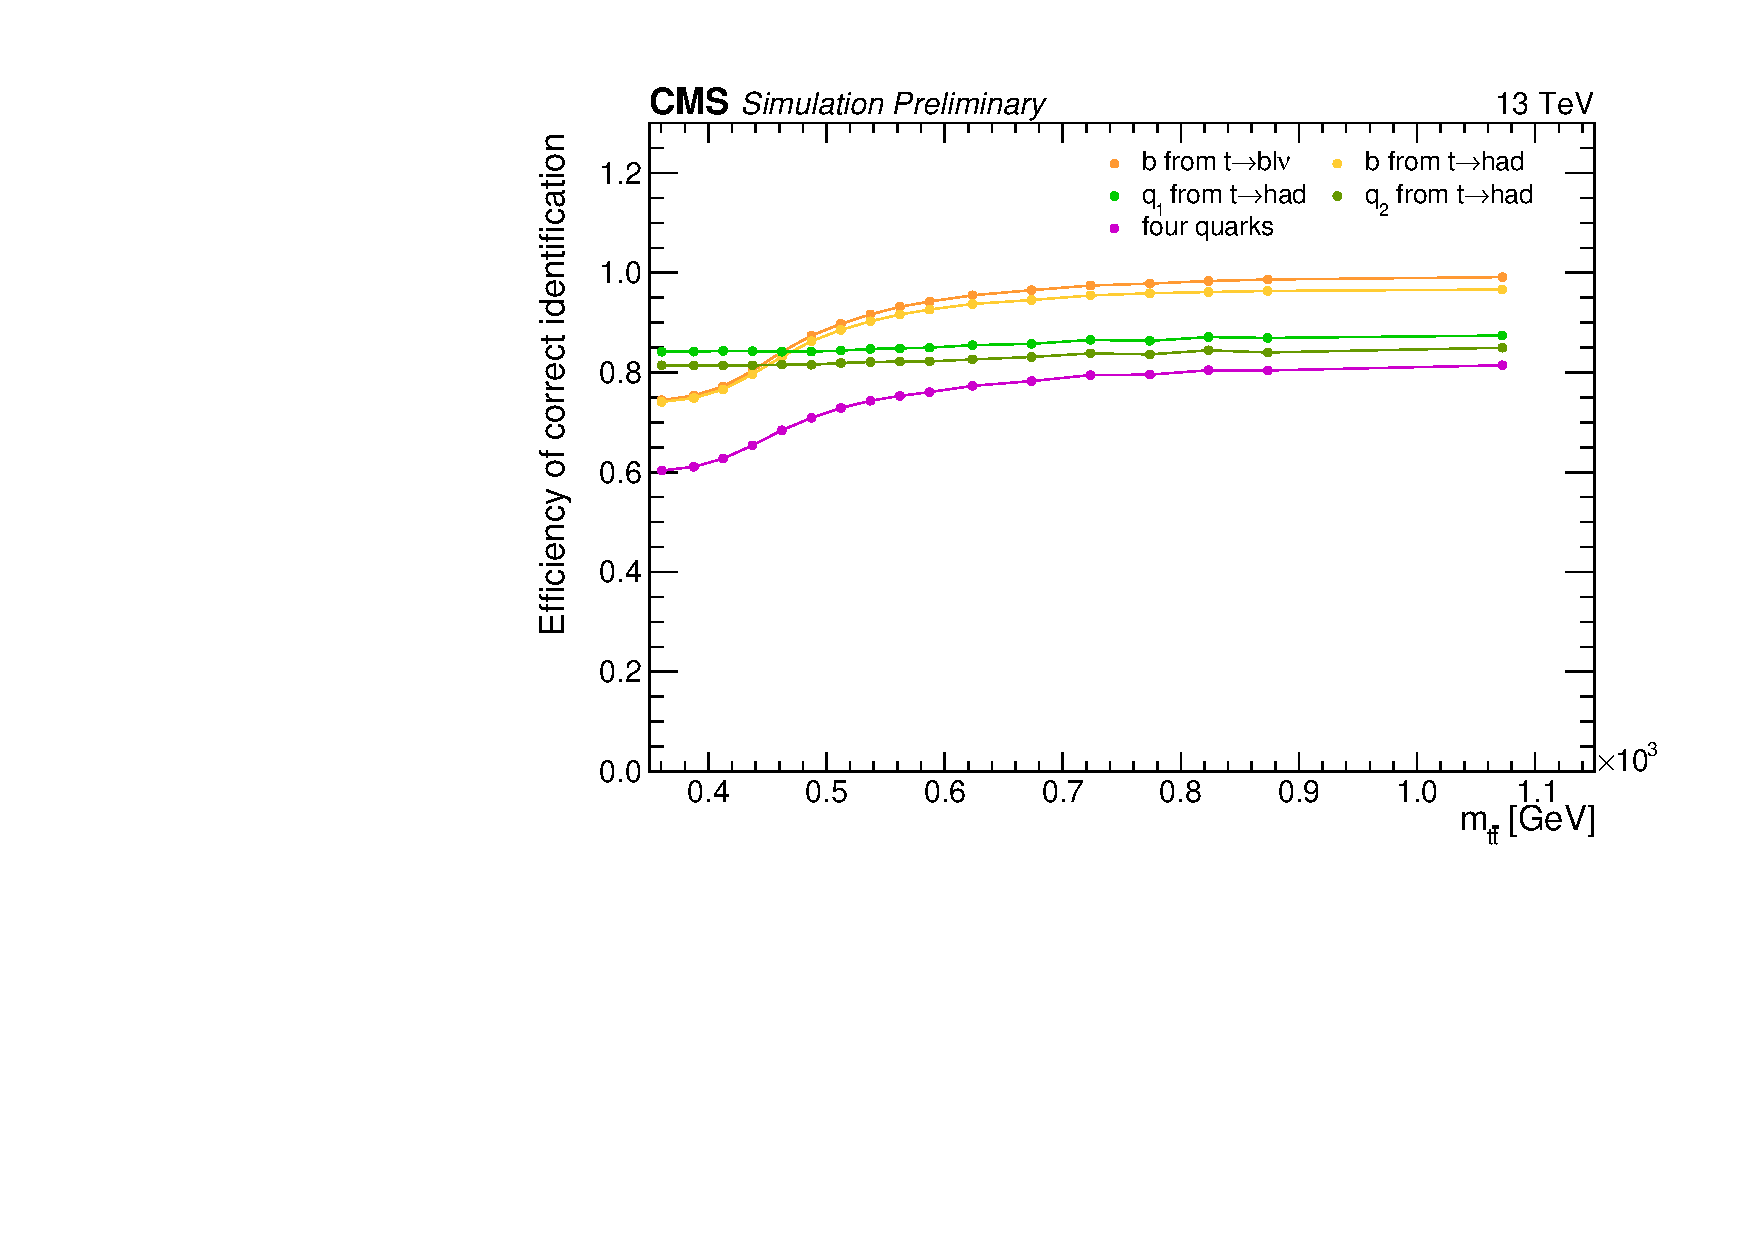
\includegraphics[width=0.45\textwidth]{fig/chapt5/perf/recoEff.pdf}
  \caption{Success rate of reconstruction of the $t\bar t$~system (left) and efficiencies of correct identification of jets stemming from various quarks in the final state of the $t\bar t$~decay (right). Shown as a function of parton-level $m_{t\bar t}$. Only fully reconstructable events are considered.}
  \label{Fig:TTRefoEff}
\end{figure}

\begin{figure}
  \centering
  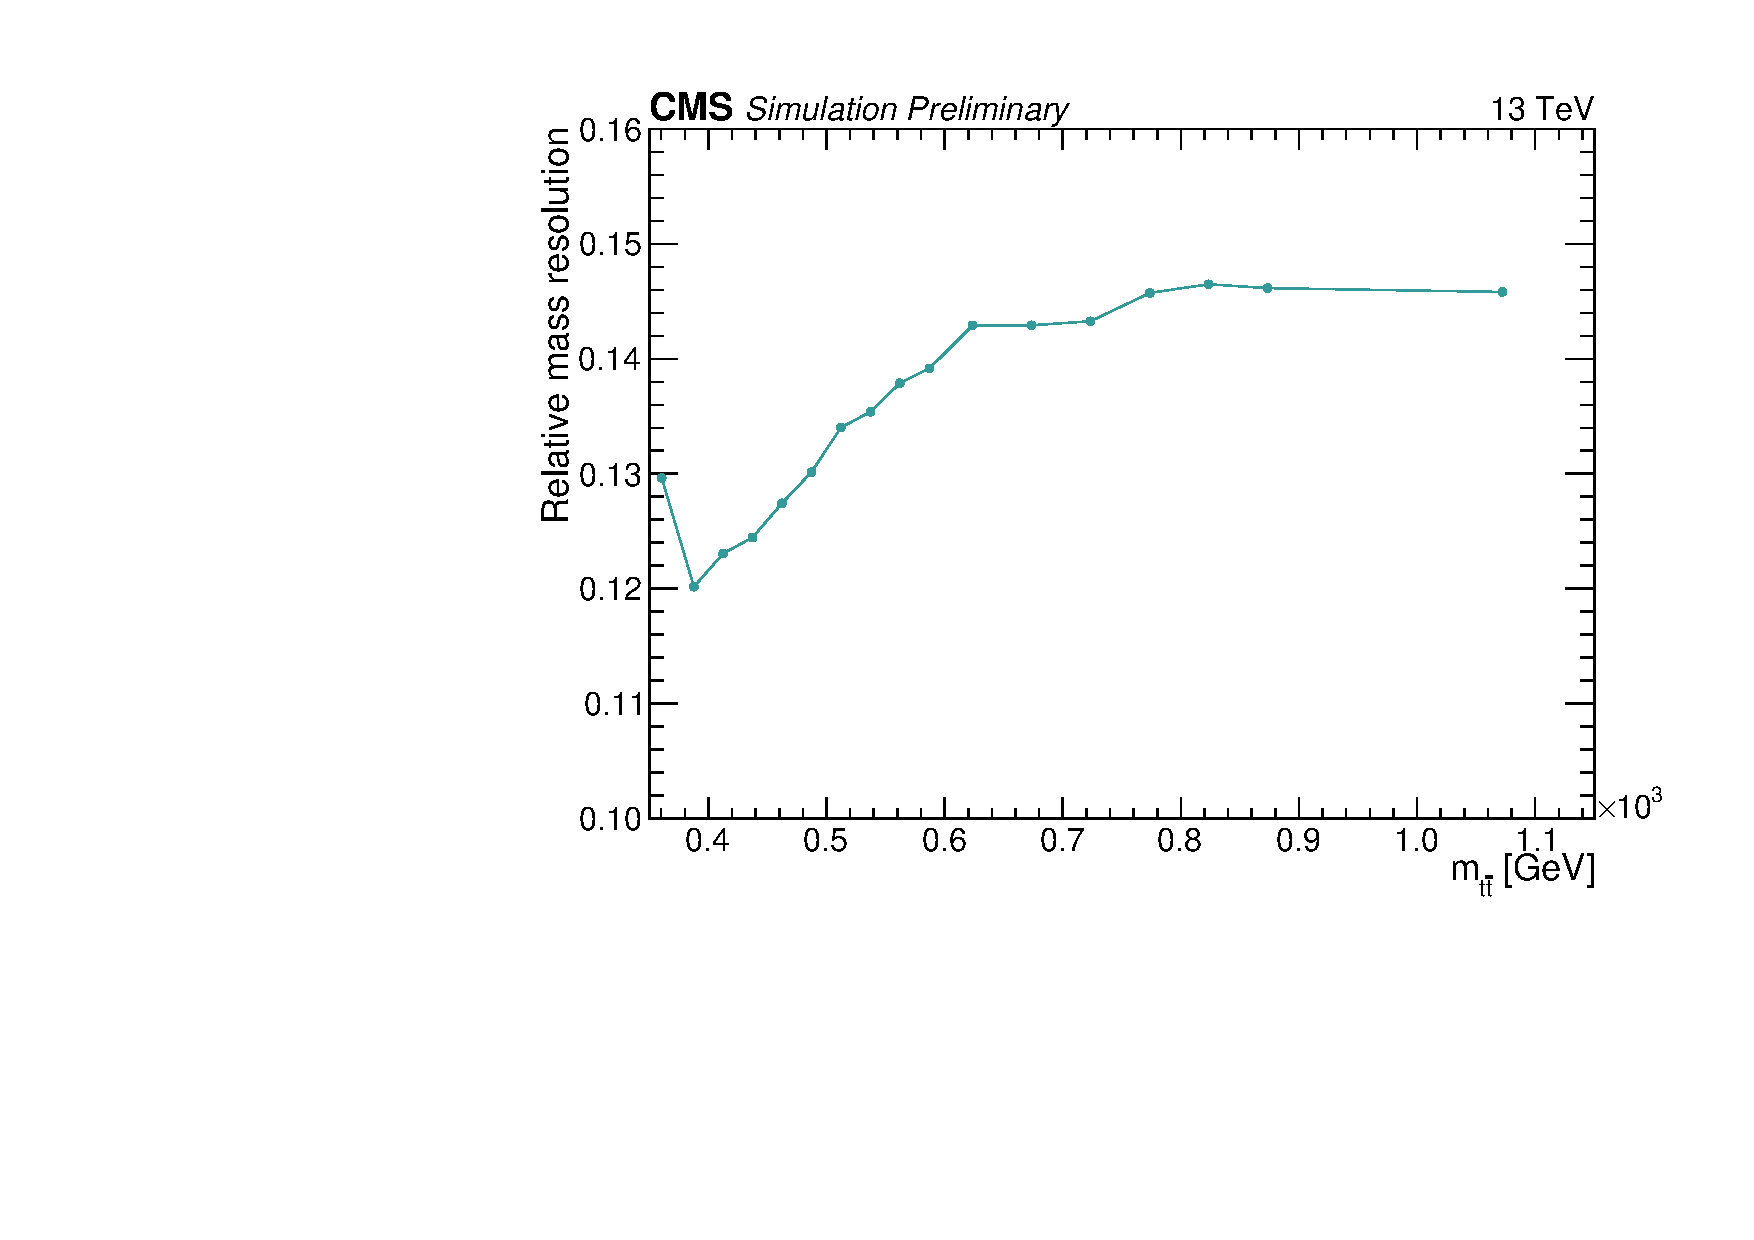
\includegraphics[width=0.45\textwidth]{fig/chapt5/perf/resolution.pdf}
  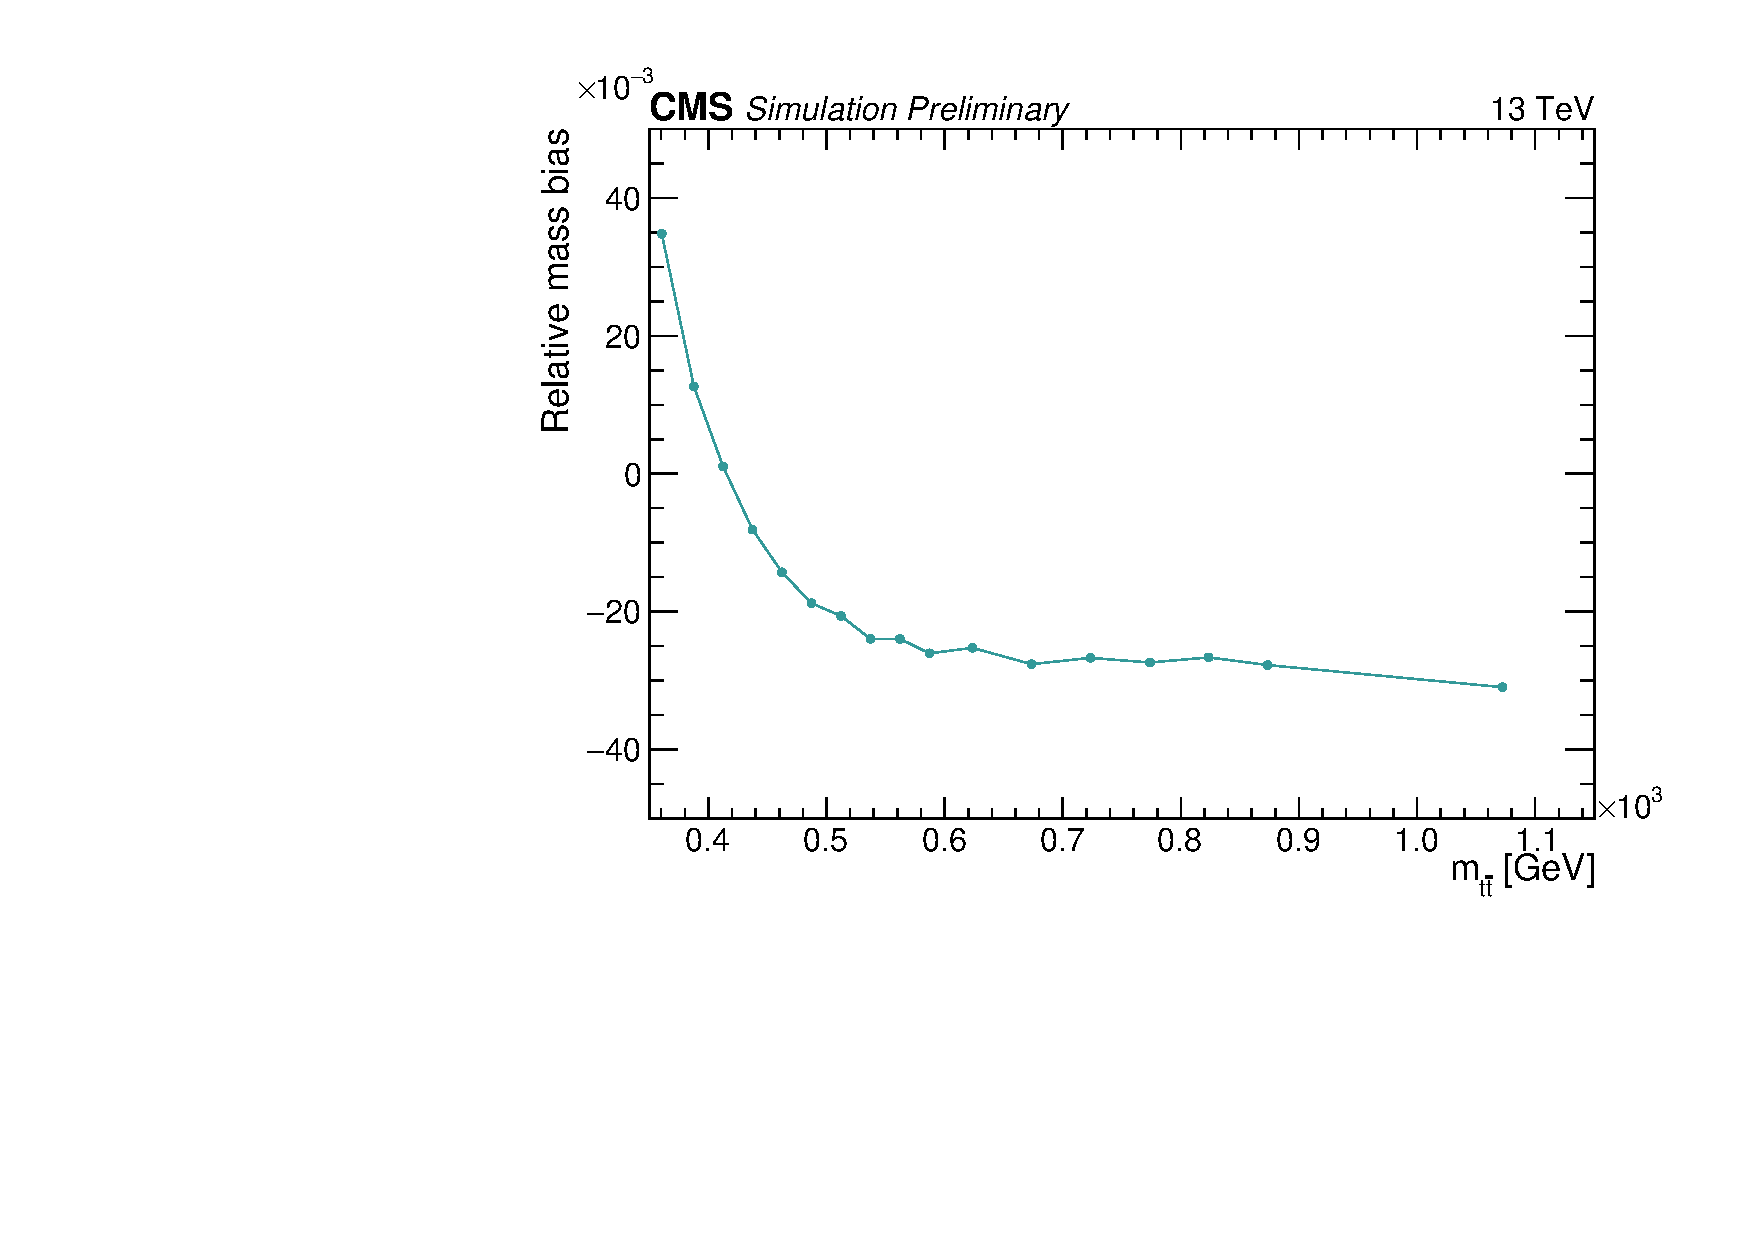
\includegraphics[width=0.45\textwidth]{fig/chapt5/perf/bias.pdf}
  \caption{Relative $m_{t\bar t}$~resolution (left) and bias (right) in fully reconstructable events.}
  \label{Fig:TTRecoMttPerf}
\end{figure}

Figure~\ref{Fig:MttSgnShapes} shows reconstructed $m_{t\bar t}$~distribution in the signal process for two example mass points.
Due to the experimental resolution, shapes for hypotheses with $\Gamma = 2.5$ and 5\% are very similar.

\begin{figure}
  \centering
  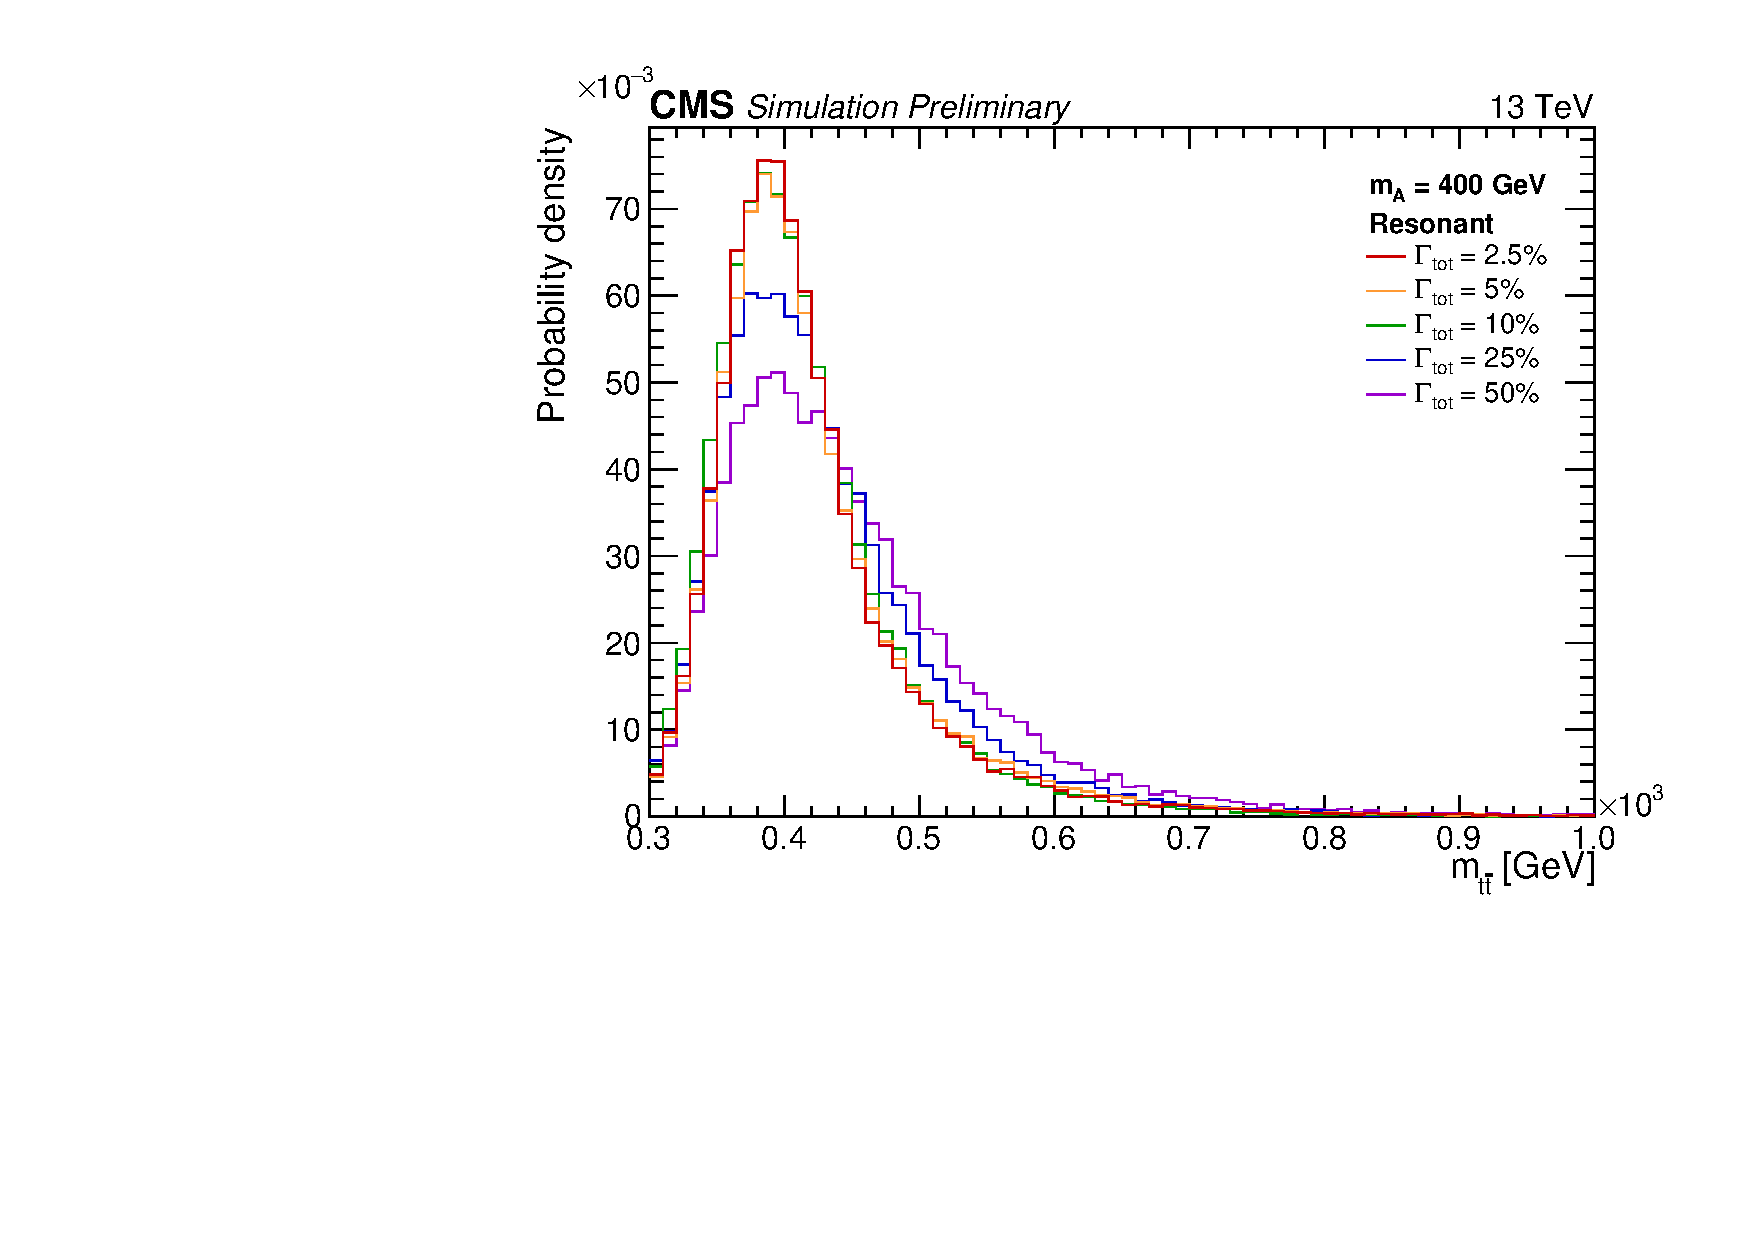
\includegraphics[width=0.45\textwidth]{fig/chapt5/sgnShapes/res/mtt_m400.pdf}
  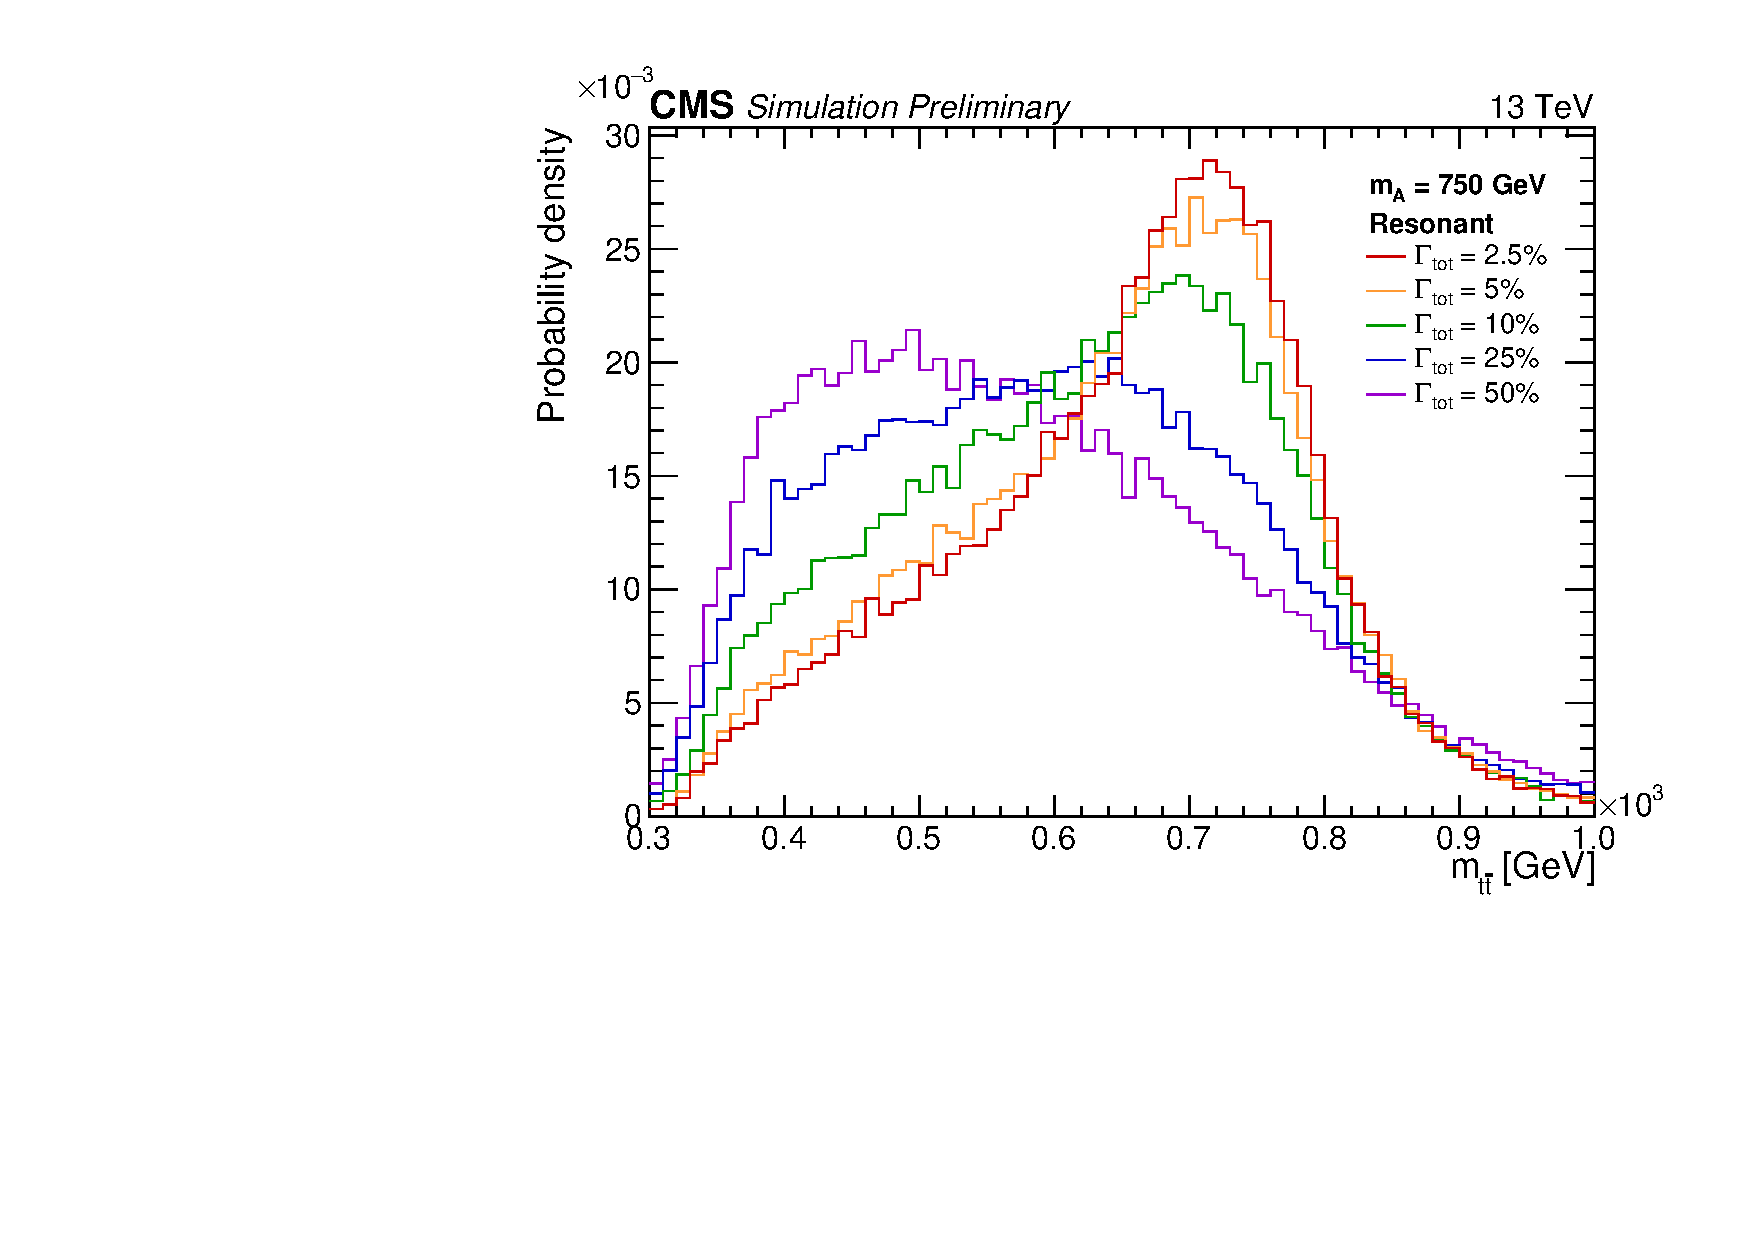
\includegraphics[width=0.45\textwidth]{fig/chapt5/sgnShapes/res/mtt_m750.pdf} \\
  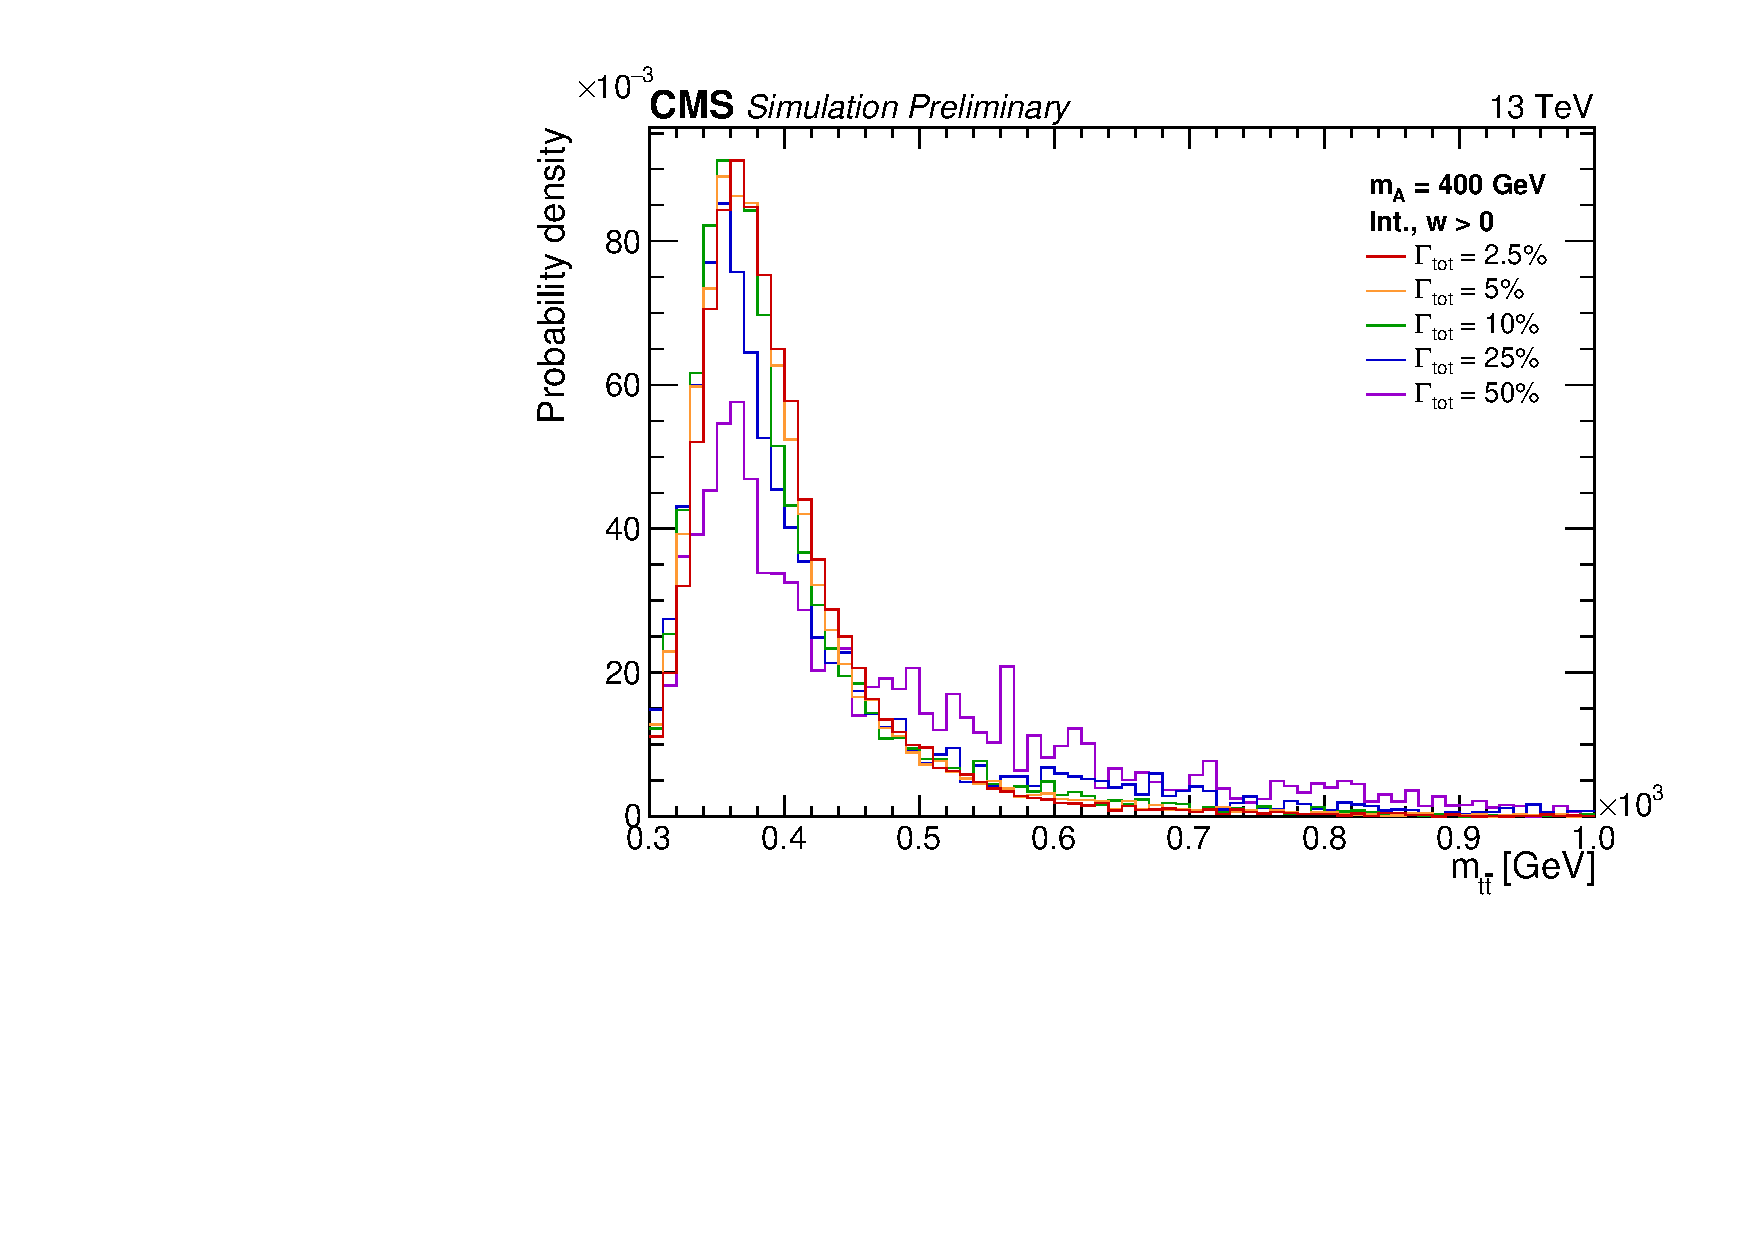
\includegraphics[width=0.45\textwidth]{fig/chapt5/sgnShapes/int/mtt_m400_pos.pdf}
  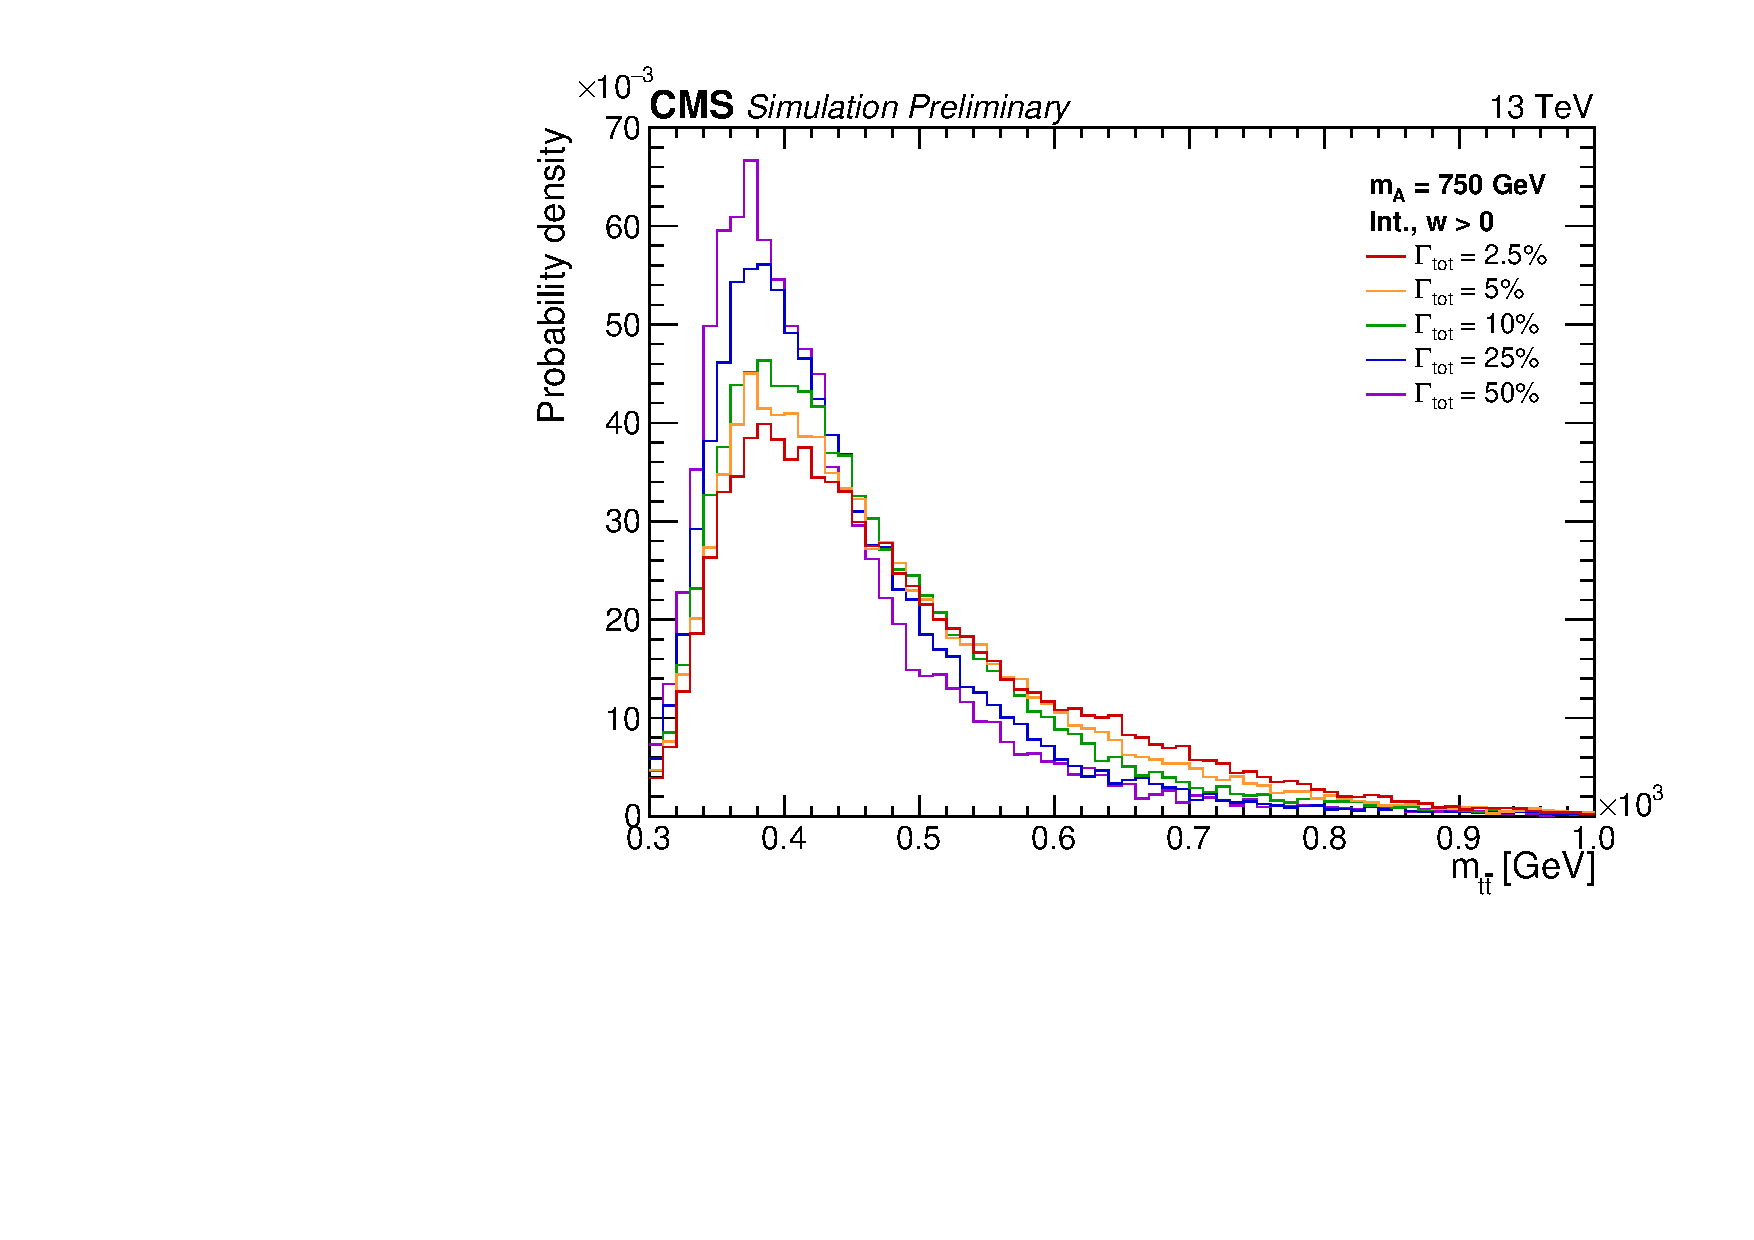
\includegraphics[width=0.45\textwidth]{fig/chapt5/sgnShapes/int/mtt_m750_pos.pdf} \\
  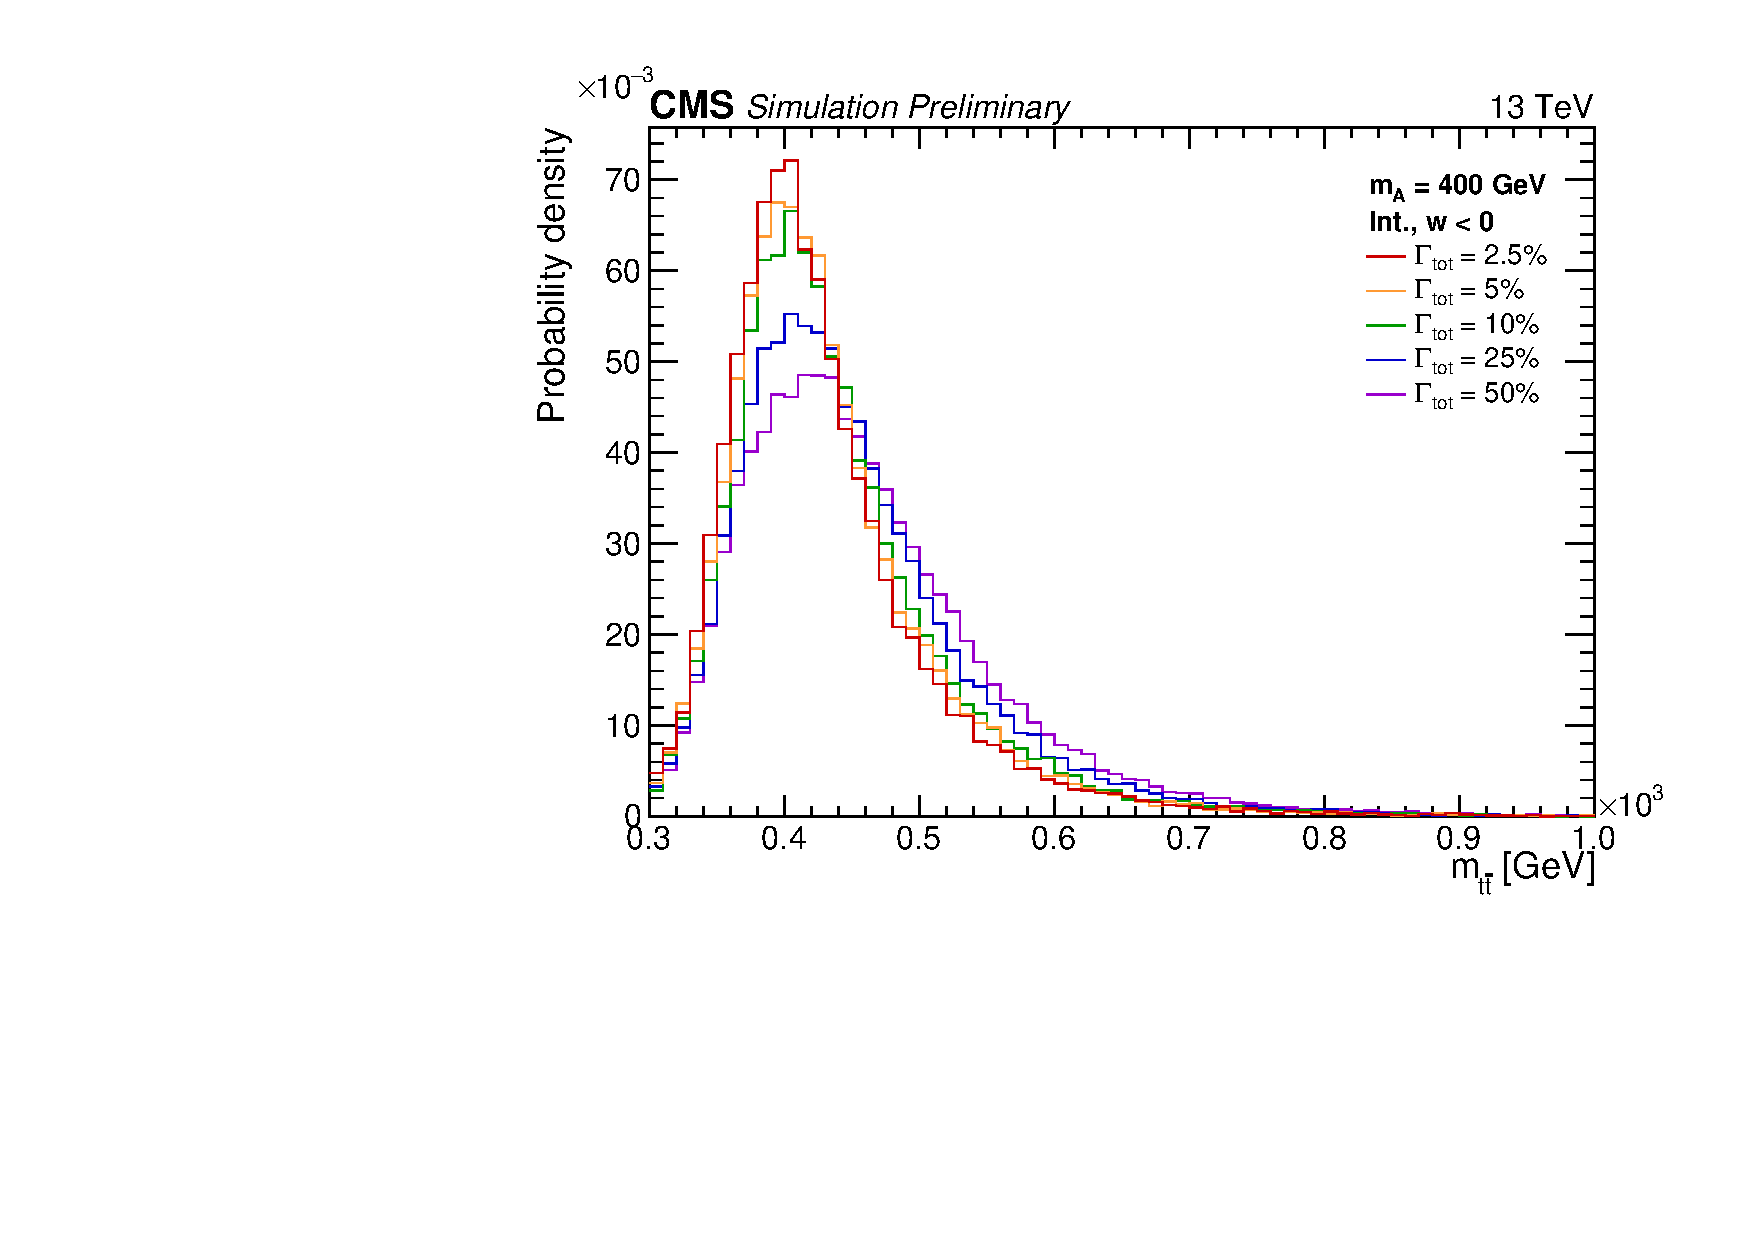
\includegraphics[width=0.45\textwidth]{fig/chapt5/sgnShapes/int/mtt_m400_neg.pdf}
  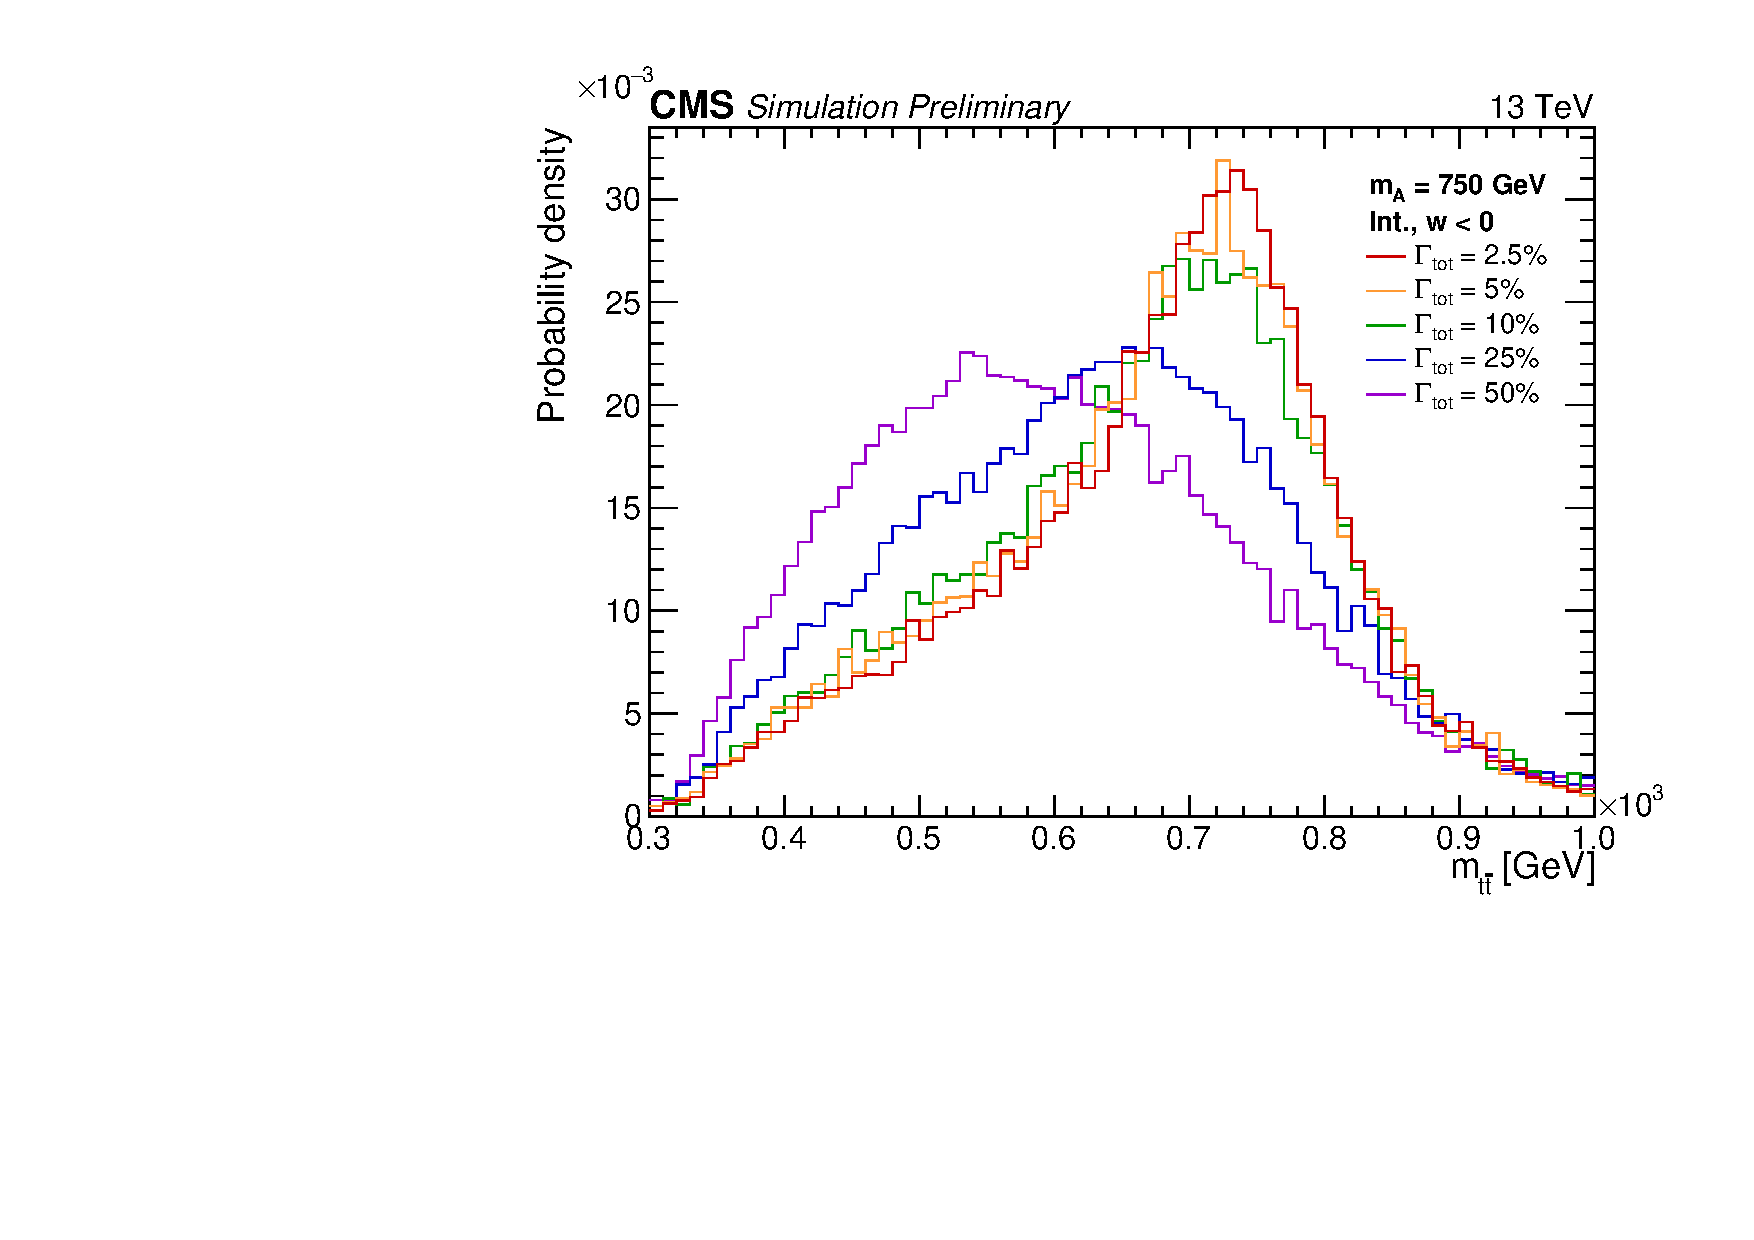
\includegraphics[width=0.45\textwidth]{fig/chapt5/sgnShapes/int/mtt_m750_neg.pdf}
  \caption{Reconstructed $m_{t\bar t}$~spectrum in resonant part of signal (top), interference with positive event weights (middle), and interference with negative weights (bottom). $\mathcal{CP}$-odd states with various total widths, $m = 400$~GeV (left) and 750~GeV (right). Distributions are normalized to unit area.}
  \label{Fig:MttSgnShapes}
\end{figure}

\subsection{Search variables}
\label{Sec:SearchVarsDef}
%
The search for $\Phi \rightarrow t\bar t$ is performed based on a joint distribution of two discriminative variables.
The first variable is the reconstructed invariant mass of the $t\bar t$~system, m$_{t\bar t}$, which serves as a proxy for the mass of the heavy Higgs boson.
In the subsequent statistical analysis its distribution is described using the non-uniform binning shown in Fig.~\ref{Fig:MttBinning}.
It has been adjusted so that the bin width is significantly smaller than the m$_{t\bar t}$~resolution everywhere except for the edges of the range.
The first and the last bins are inclusive.

\begin{figure}
  \centering
  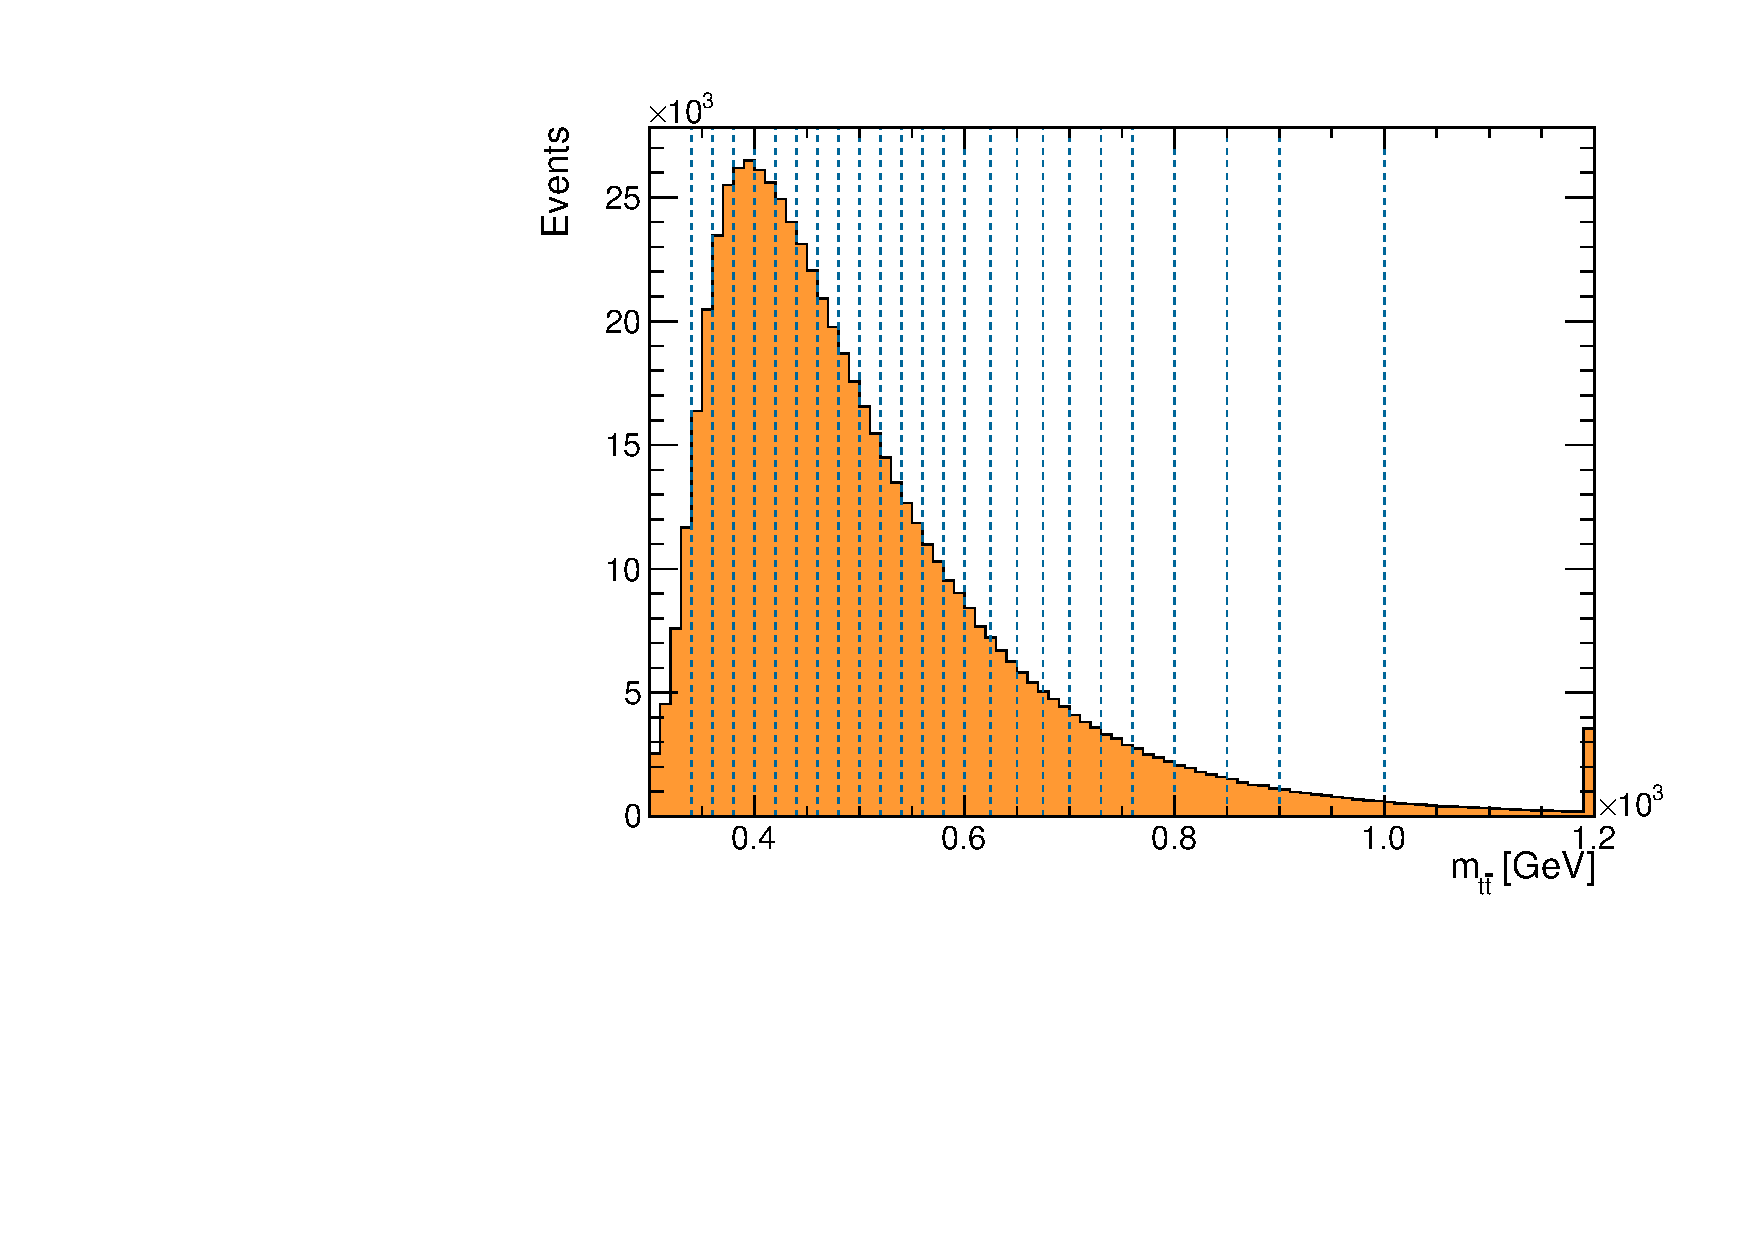
\includegraphics[width=0.45\textwidth]{fig/chapt5/searchVars/mtt-bins.pdf}
  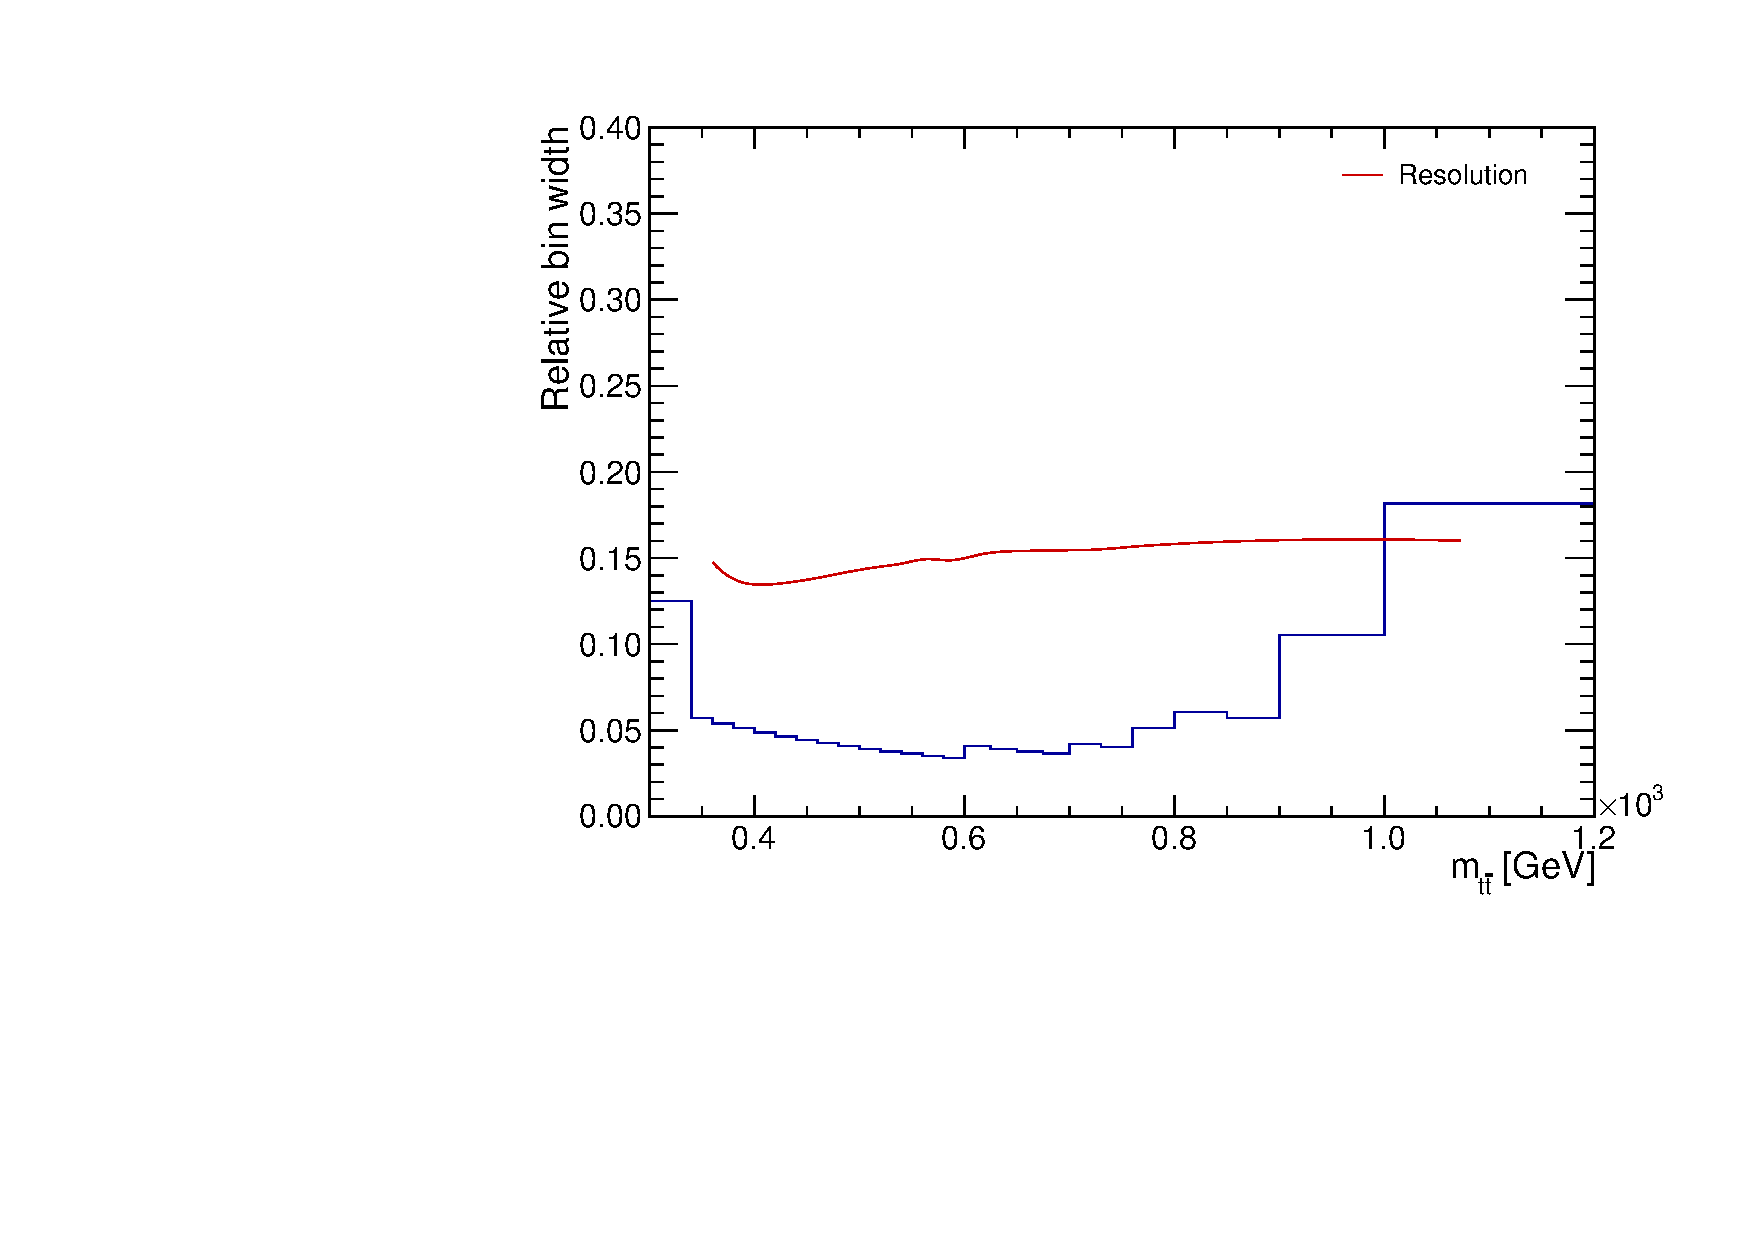
\includegraphics[width=0.45\textwidth]{fig/chapt5/searchVars/mtt-bin-width.pdf}
  \caption{Optimized binning in m$_{t\bar t}$, superimposed over the distribution of SM $t\bar{t}$, (left) and relative bin width compared to the m$_{t\bar t}$~resolution (right).}
  \label{Fig:MttBinning}
\end{figure}

The second variable is $\abs{\cos\theta^*}$, where $\theta^*$ is the angle between the three-momentum of the leptonically decaying top quark in the $t\bar{t}$ rest frame and the three-momentum of the $t\bar{t}$~system in the lab frame.
In the (resonant part of the) signal process the distribution of this variable reflects the fact that the Higgs boson is a scalar particle and therefore decays into top quarks isotropically.
On the other hand, the distribution for the SM~$t\bar{t}$ production has a non-trivial shape peaking at $\abs{\cos\theta^*} = 1$ (see Ref.~\cite{Dicus:1994bm} and references therein), which in part is driven by the contribution with the $s$-channel gluon exchange.

As illustrated in Fig.~\ref{Fig:CosThetaStar}, the reconstructed distribution of $\cos\theta^*$ is not symmetric.
However, the ratio between distributions of the signal process and the SM~$t\bar{t}$ background is approximately symmetric, which allows to consider in the analysis only the absolute value of the observable without a loss of sensitivity.
The binning used for the statistical analysis is adjusted to minimize the variation of the ratio within each bin, so that regions over which the ratio changes slowly are covered by wider bins.
The following bin edges have been chosen: 0., 0.4, 0.6, 0.75, 0.9, 1.

\begin{figure}
  \centering
  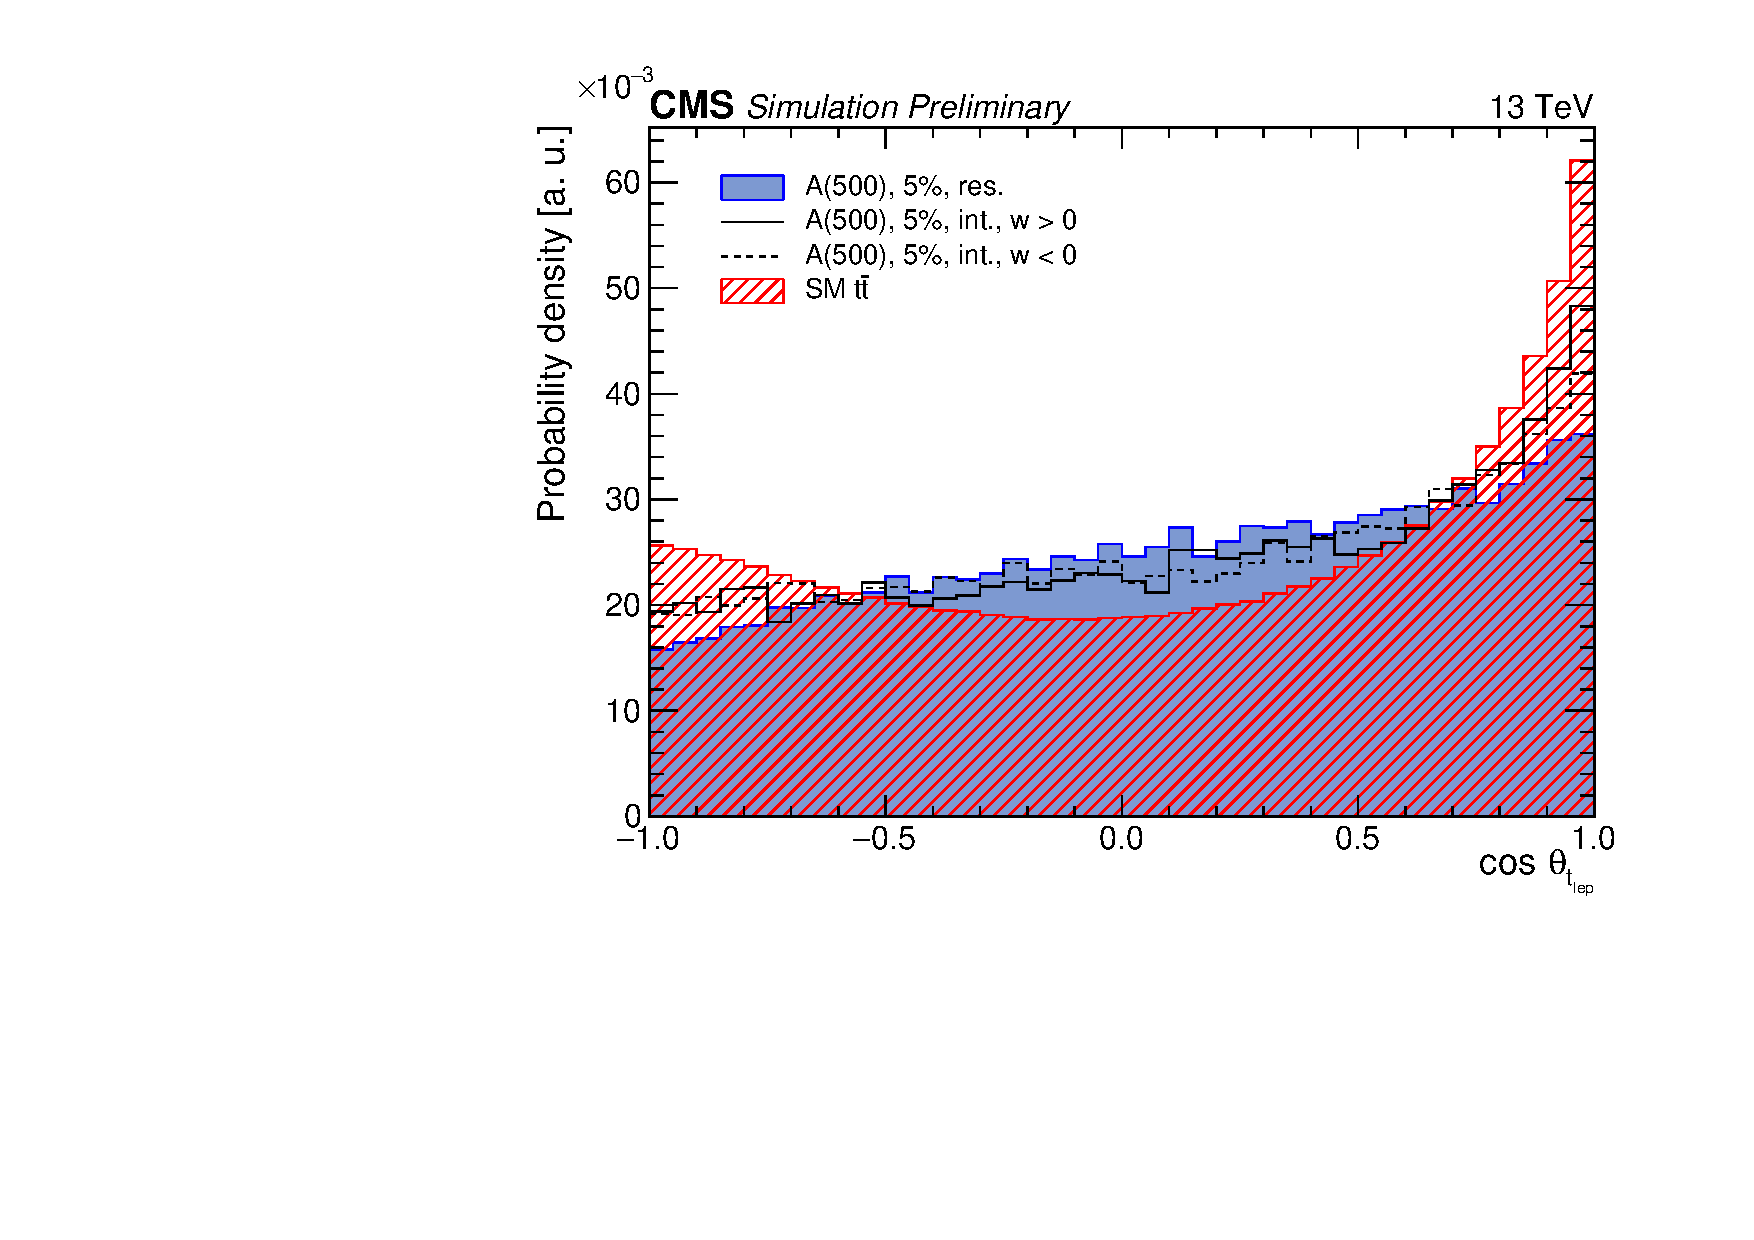
\includegraphics[width=0.45\textwidth]{fig/chapt5/searchVars/CosTopLepTT.pdf}
  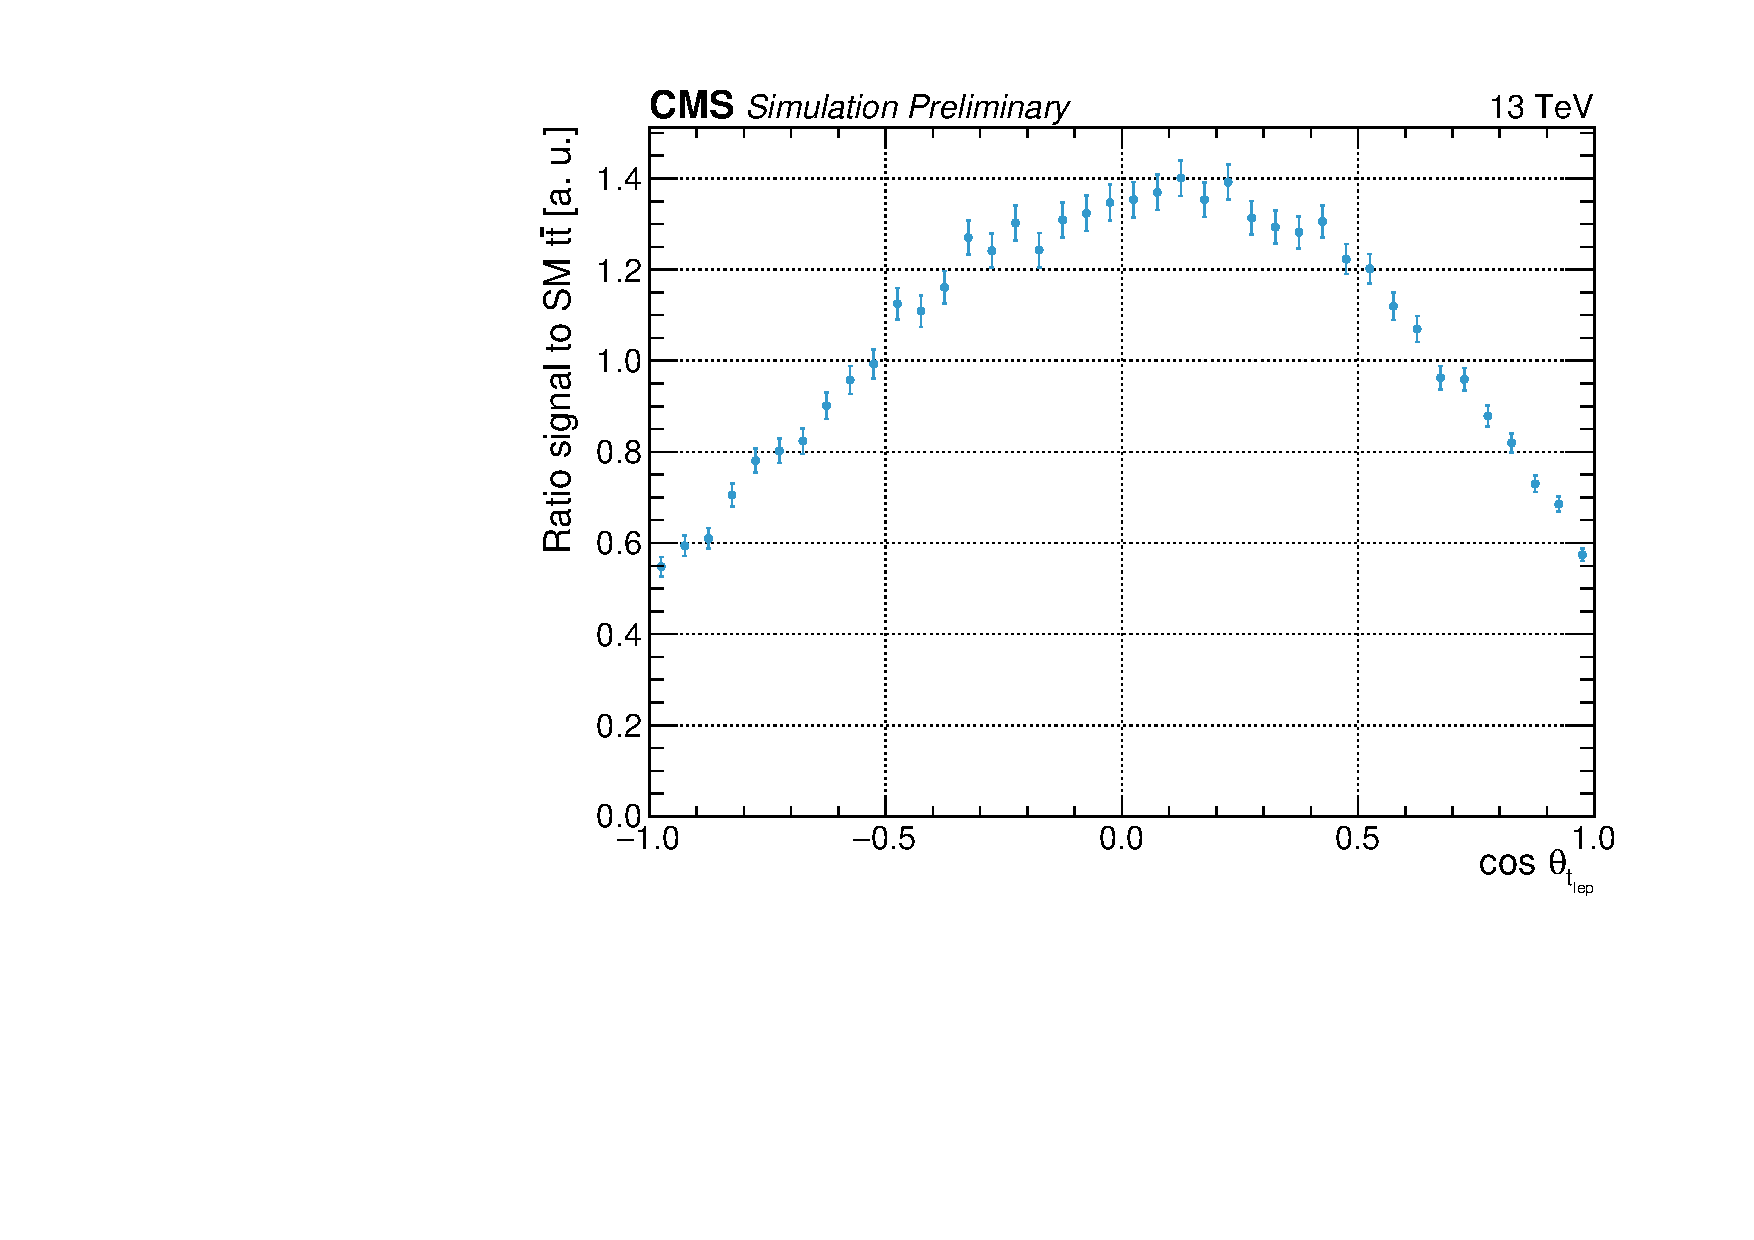
\includegraphics[width=0.45\textwidth]{fig/chapt5/searchVars/CosTopLepTT_ratio.pdf}
  \caption{Distribution of $\cos\theta^*$ in an example signal process for resonance, positive and negative interference and the SM~$t\bar{t}$ background (left) and the ratio between the pure resonance and the SM~$t\bar{t}$ background (right).}
  \label{Fig:CosThetaStar}
\end{figure}

\section{Data-driven modelling of the multijet background}
\label{Sec:DataDrivenQCD}
%
One of the main background for semi-leptonic $t\bar{t}$ decays is the multijet QCD that has overwhelming cross section. Due to tight selection criteria, only a small fraction of these events mimics the semi-leptonic final state. This requires large simulation samples to have proper QCD modelling and enough statistics after the final selection that is not practical. We used data-driven technique to model our multijet QCD where we defined sideband regions in data that are enriched in QCD events. The number of events stemming from the multijet background and the distributions of the relevant kinematic variables for final fit are taken directly from these data. The mass of $t\bar{t}$ and $\abs{\cos\theta^*}$ are used as normalization variables. In semi-leptonic decays of $t\bar{t}$, the multijet QCD background can mimic the signal via two main processes.
\begin{itemize}
\item Non-prompt and less isolated leptons from the decay of beauty and charm quarks. These are real leptons that gain significant $p_{T}$ from the mother b and c hadrons and have more activities in the vicinity. Lepton isolation cut suppresses these events.
\item Some hadrons didn't absorbed in the HCAL and make tracks in the muon system or jets with high electromagnetic fraction mimics electron signatures. They are treated as fake leptons.  
\end{itemize}

\subsection{Normalization}
%
The number of events from the multijet background is estimated with the so-called ABCD method (see, for instance, a review in Ref.~\cite{Loginov:2010zz}), independently in the muon and electron channels.
% Could not find a proper reference for the method. The earliest usage I found is from 2005, used in CDF: arXiv:hep-ex/0508029. In CMS it was used as early as EWK-07-002 and TOP-08-005.
The method is applied for the $M_{T}^W$ variable~\ref{Eq:MtW} and the lepton's relative isolation~$I$, which in case of muons is defined by Eq.~\ref{Eq:IsolationDeltaBeta}, while for electrons the $\rho$-corrected isolation included in the identification criterion is exploited.
Four regions are defined based on these variables as sketched in Fig.~\ref{Fig:ABCD_plane}.
Region~A is the signal region with an additional requirement of a successful $t\bar t$~reconstruction.
Region~C is built from it by inverting the $M_{T}^W$ selection: $m_\text{T}^W < 50$~GeV.
Complementarily, region~B is defined by inverting the isolation requirement: $I > 0.15$ for muons and $I > 0.0588$ (0.0571) for electrons in the barrel (endcaps).
This inversion, however, requires a change to the logic of the lepton step of the event selection.
In the definition of tight leptons in Sec.~\ref{Sec:Reconstruction} the isolation requirement is removed, and such a lepton with the highest~$p_{T}$ in an event must satisfy the aforementioned lower cut on the isolation.
The event must also contain no additional loose leptons according to the standard definition.
Jets are removed if they overlap with a loose lepton (of which there can be zero or one in an event, depending on the isolation of the selected lepton).
Finally, region~D is constructed from region~A by inverting both $M_{T}^W$ and isolation requirements.
Since the selections on the isolation and $M_{T}^W$ have been designed to suppress the multijet background, inversion of any of them increases its contribution.
The fractions of events from each background source expected in the different regions are reported in Tables~\ref{table:ABCD_fractions_semimu} and \ref{table:ABCD_fractions_semie}.

\begin{figure}
  \centering
  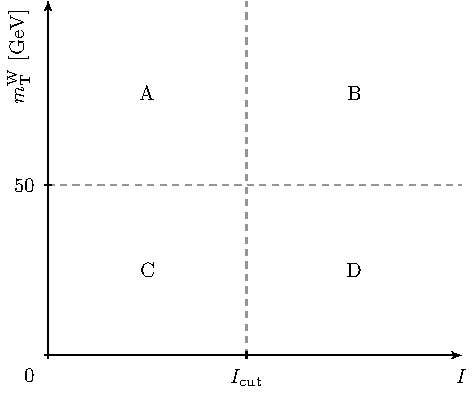
\includegraphics[width=0.5\textwidth]{fig/chapt6/normalisation/ABCD-sketch.pdf}
  \caption{Schematic representation of the four regions used for the evaluation of the number of multijet events entering the signal region.}
  \label{Fig:ABCD_plane}
\end{figure}

\begin{table}
  \caption{Fractions of events from each background source in the four regions used to evaluate the multijet background normalization. Muon channel.}
  \centering
  \begin{tabular}{lcccc}
    \hline
    \hline
    \multicolumn{1}{c}{Process} & A  & B  & C  & D \\
    \hline
    Multijet    & 0.01     & 0.21     & 0.06     & 0.67    \\
    $t\bar t$      & 0.92     & 0.75     & 0.88     & 0.31    \\
    Single top  & 0.02     & 0.02     & 0.02     & $<0.01$ \\
    W         & 0.04     & 0.03     & 0.04     & 0.01    \\
    Other       & $<0.01$  & $<0.01$  & $<0.01$  & $<0.01$ \\
    \hline
    \hline
  \end{tabular}
  \label{table:ABCD_fractions_semimu}
\end{table}

\begin{table}
  \caption{Fractions of events from each background source in the four regions used to evaluate the multijet background normalization. Electron channel.}
  \centering
  \begin{tabular}{lcccc}
    \hline
    \hline
    \multicolumn{1}{c}{Process} & A  & B  & C  & D \\
    \hline
    Multijet    & 0.01     & 0.16     & 0.04     & 0.31    \\
    $t\bar t$      & 0.92     & 0.78     & 0.89     & 0.64    \\
    Single top  & 0.02     & 0.02     & 0.02     & 0.01    \\
    W         & 0.04     & 0.04     & 0.04     & 0.03    \\
    Other       & $<0.01$  & $<0.01$  & $<0.01$  & $<0.01$ \\
    \hline
    \hline
  \end{tabular}
  \label{table:ABCD_fractions_semie}
\end{table}

The ABCD method determines the number of events from the multijet background in the signal region, $n_A^\text{QCD}$, using an assumption that the two variables are not correlated for this background, which gives
\begin{linenomath}
\begin{equation}
  n_{A}^\text{QCD} = \frac{n_{B}^\text{QCD} \cdot n_{C}^\text{QCD}}{n_{D}^\text{QCD}}.
  \label{Eq:ABCD_formula}
\end{equation}
\end{linenomath}
The assumption of no correlation is verified with MC simulation and is demonstrated to hold within statistical uncertainties:
\begin{linenomath}
\begin{equation*}
\begin{gathered}
  \frac{n_{A}^\text{QCD}}{n_{C}^\text{QCD}}=0.35 \pm 0.13, \quad \frac{n_{B}^\text{QCD}}{n_{D}^\text{QCD}}=0.25\pm 0.07 \quad \text{in muon channel}, \\
  \frac{n_{A}^\text{QCD}}{n_{C}^\text{QCD}}=0.53 \pm 0.22, \quad \frac{n_{B}^\text{QCD}}{n_{D}^\text{QCD}}=0.93\pm 0.45 \quad \text{in electron channel}.
\end{gathered}
\end{equation*}
\end{linenomath}
This conclusion is further supported by Fig.~\ref{Fig:RelIso_mtWcut}, which shows that distributions of the relative isolation agree between the two regions in $M_{T}^W$.

\begin{figure}
  \centering
  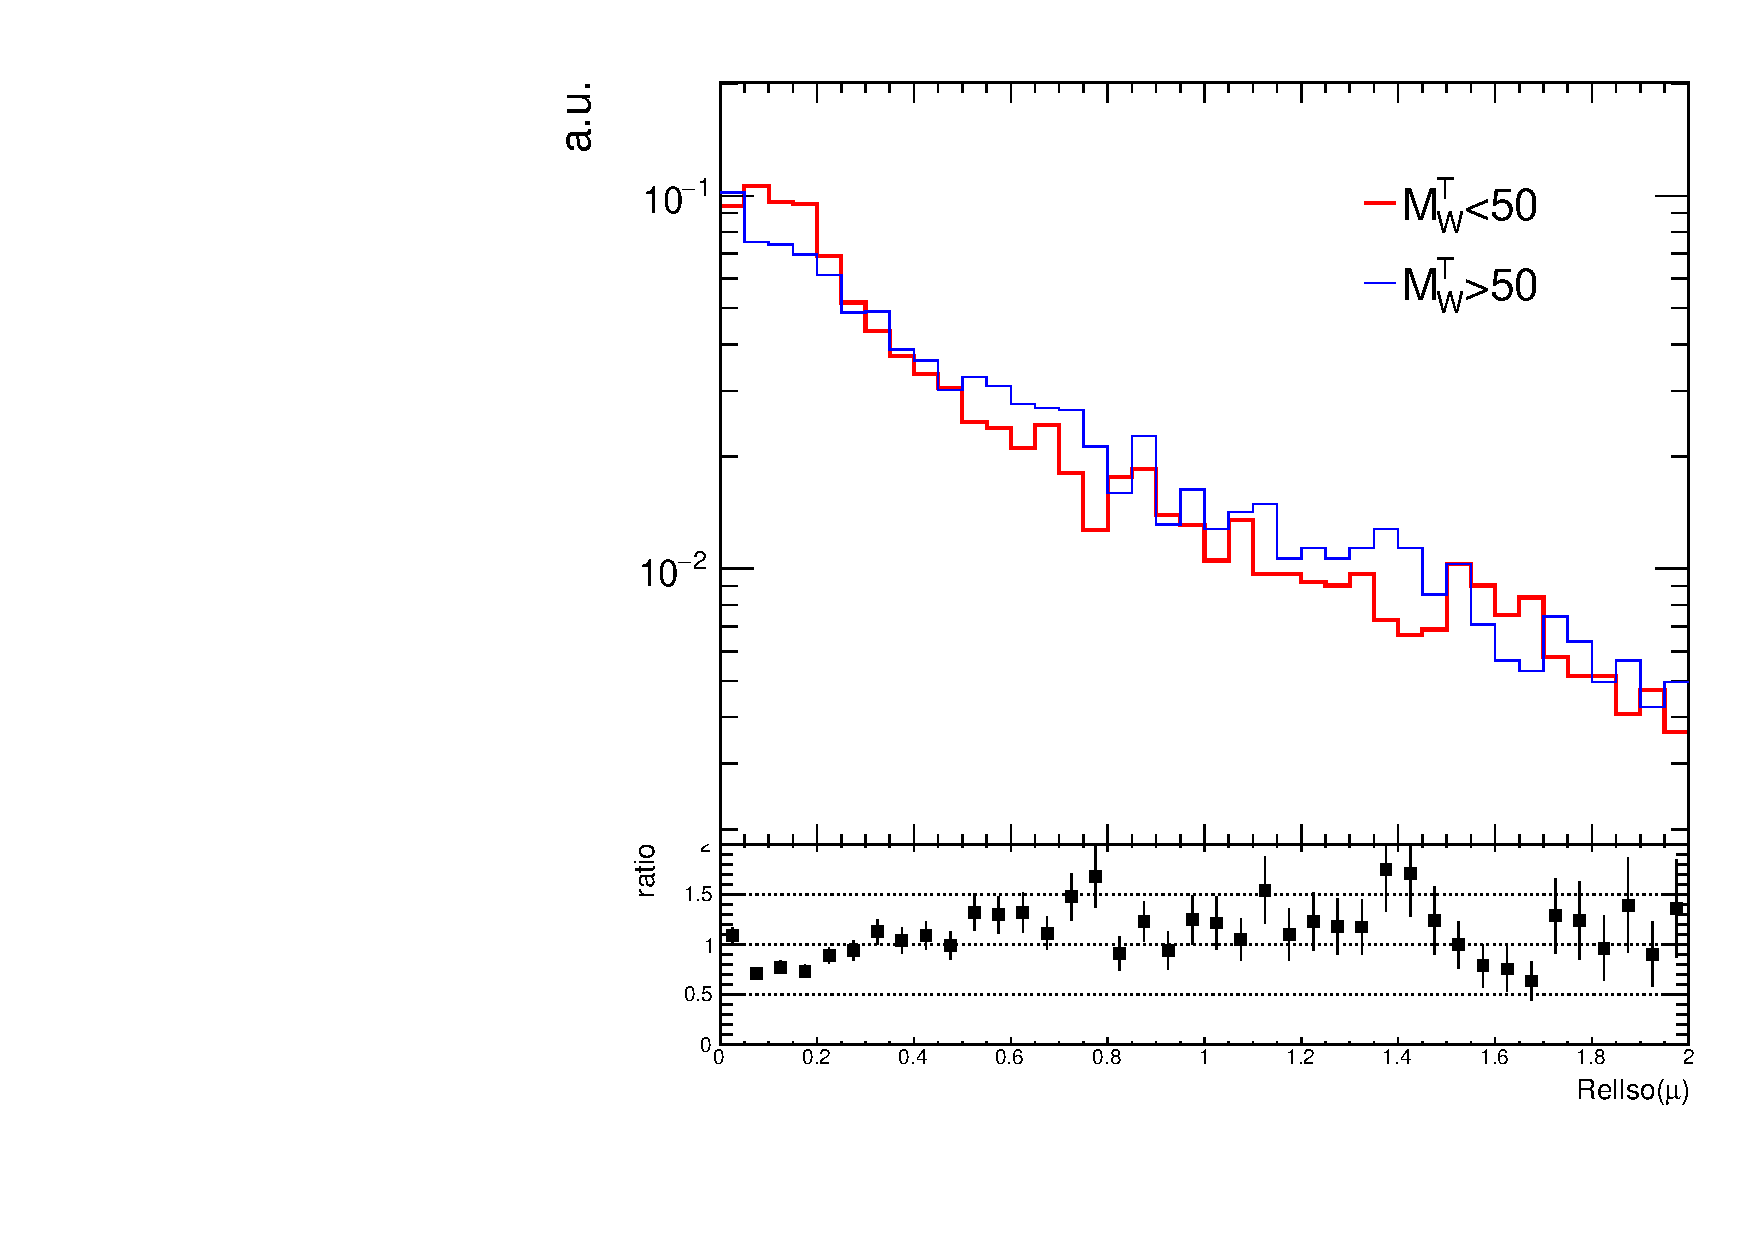
\includegraphics[width=0.45\textwidth]{fig/chapt6/normalisation/RelIso_mtWcut_semimu}
  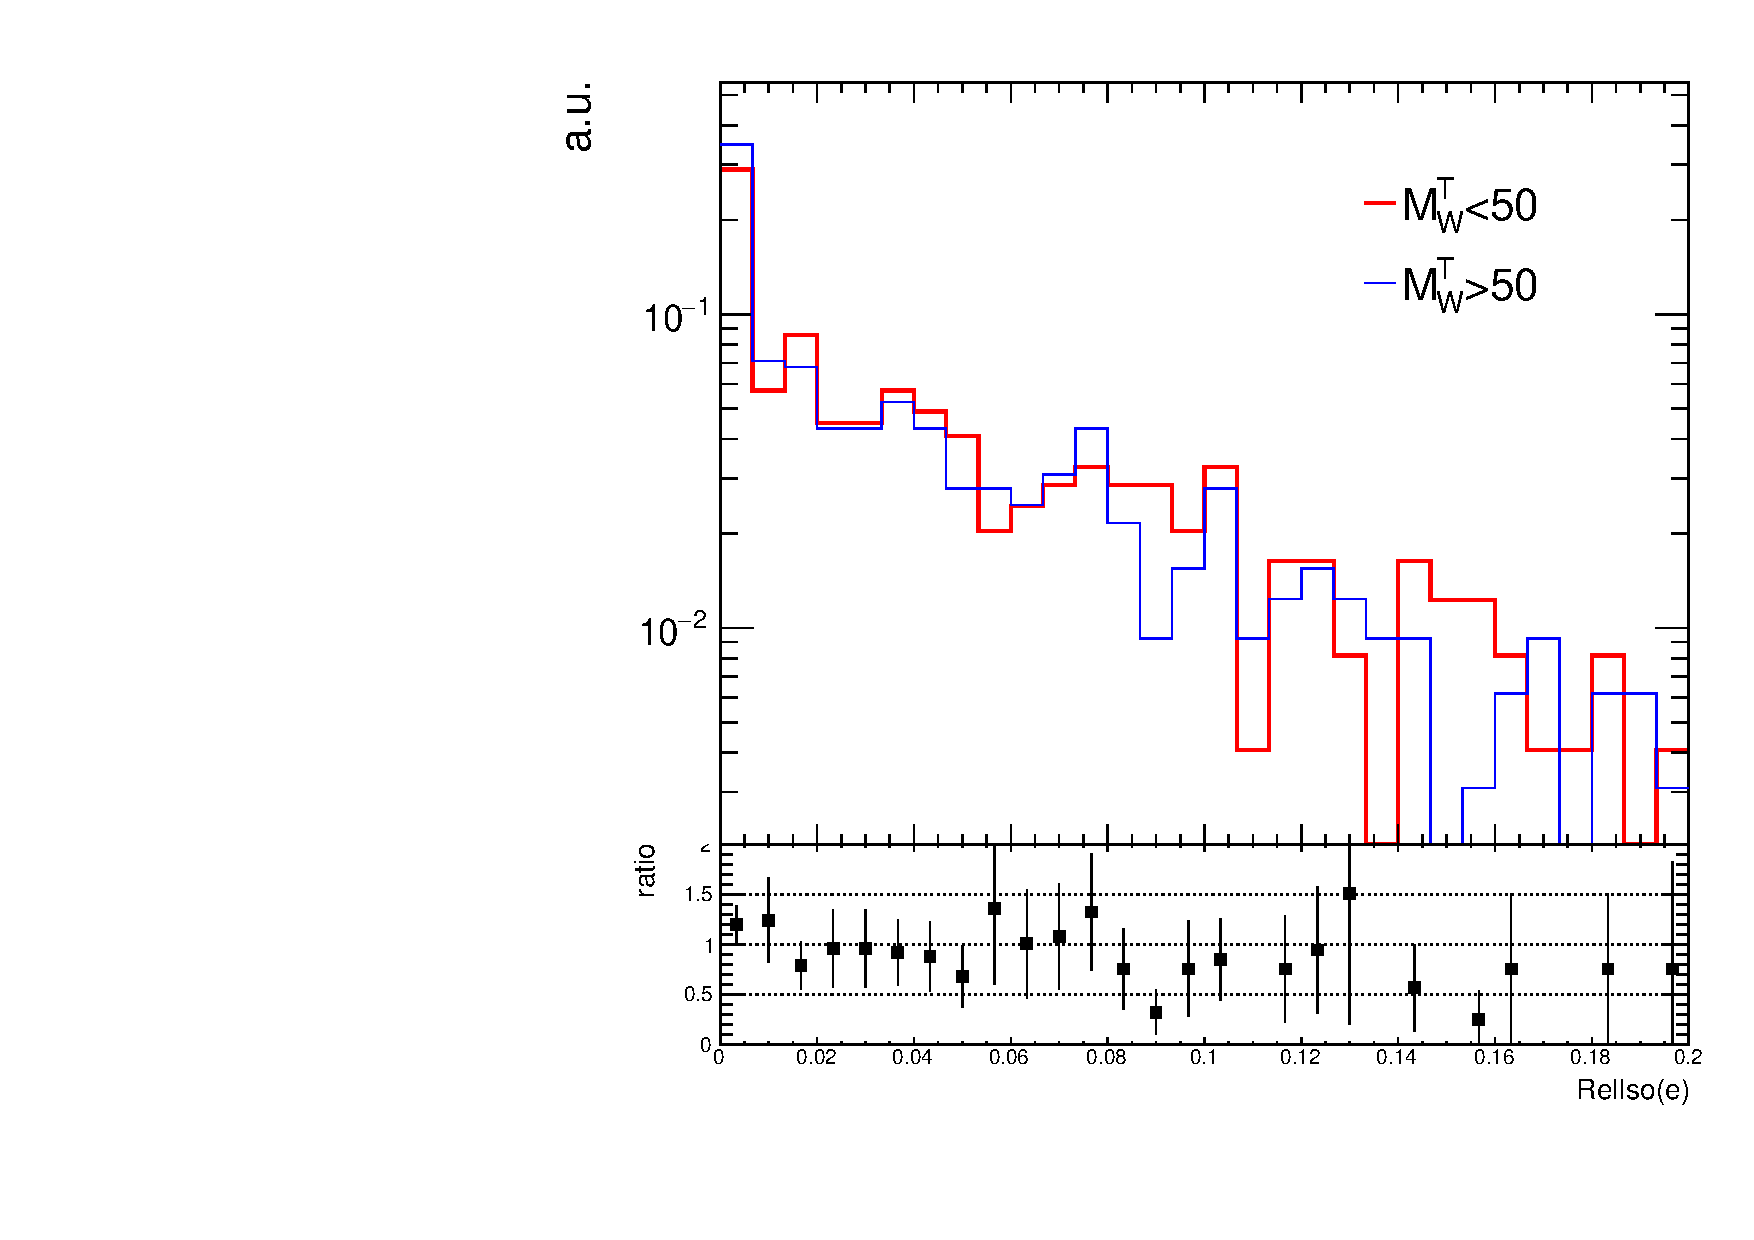
\includegraphics[width=0.45\textwidth]{fig/chapt6/normalisation/RelIso_mtWcut_semie}
  \caption{Distributions of the lepton's relative isolation, for events satisfying the nominal $M_{T}^W$~selection and the inverted one, in the muon (left) and electron (right) channels using MC simulation.}
  \label{Fig:RelIso_mtWcut}
\end{figure}

Figure~\ref{Fig:DataMC_reliso_mtw} shows distributions of variables~$I$ and $M_{T}^W$ in data and simulation, and they demonstrate a reasonable agreement.
The excess of data for large values of the isolation in case of the electron channel is attributed to the way the simulated samples for the multijet background have been produced.
The samples are enriched in events with higher electromagnetic activity, and the corresponding generator-level filter (\texttt{EMEnrichingFilter}) includes a loose isolation requirement.
This results in a deficit in simulation for large values of the isolation.
In Figs.~\ref{Fig:DataMC_ABCD_semimu} and \ref{Fig:DataMC_ABCD_semie} distributions of an example observable (the transverse momentum of the hadronically decaying top quark) in the four regions are shown.

\begin{figure}
  \centering
  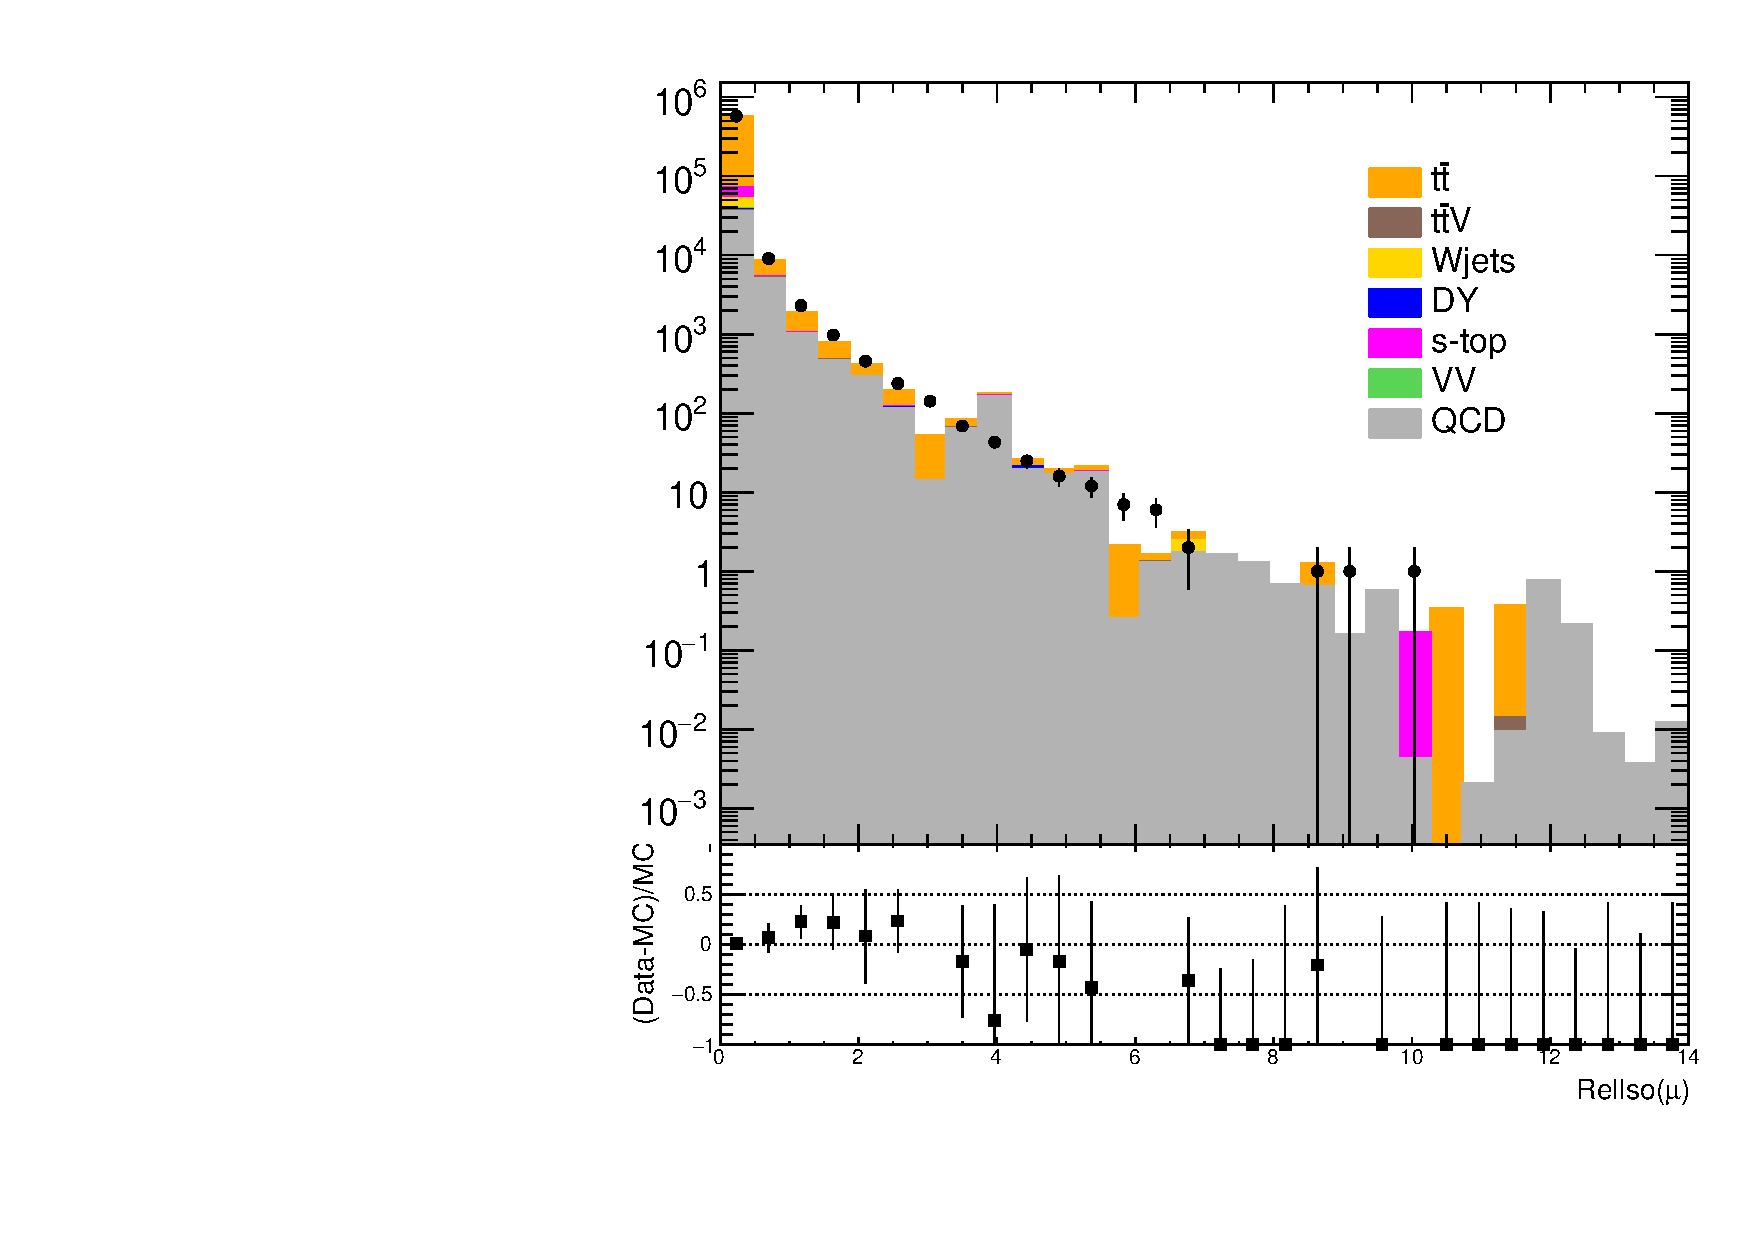
\includegraphics[width=0.45\textwidth]{fig/chapt6/normalisation/dataMC_reliso_semimu.pdf}
  \includegraphics[width=0.45\textwidth]{fig/chapt6/normalisation/dataMC_mTW_semimu.pdf} \\
  \includegraphics[width=0.45\textwidth]{fig/chapt6/normalisation/dataMC_reliso_semie.pdf}
  \includegraphics[width=0.45\textwidth]{fig/chapt6/normalisation/dataMC_mTW_semie.pdf}
  \caption{Distributions of $I$ (left) and $M_{T}^W$ (right) in the muon (top) and electron (bottom) channels.}
  \label{Fig:DataMC_reliso_mtw}
\end{figure}

\begin{figure}
  \centering
  \includegraphics[width=0.45\textwidth]{fig/chapt6/normalisation/dataMC_pt_thad_A_semimu.pdf}
  \includegraphics[width=0.45\textwidth]{fig/chapt6/normalisation/dataMC_pt_thad_C_semimu.pdf} \\
  \includegraphics[width=0.45\textwidth]{fig/chapt6/normalisation/dataMC_pt_thad_B_semimu.pdf}
  \includegraphics[width=0.45\textwidth]{fig/chapt6/normalisation/dataMC_pt_thad_D_semimu.pdf}
  \caption{Distributions of the $p_{T}$ of the hadronically decaying top quark in the four regions used to estimate the normalization of the multijet background (from left to right, top to bottom: A, B, C, and D). Muon channel.}
  \label{Fig:DataMC_ABCD_semimu}
\end{figure}

\begin{figure}
  \centering
  \includegraphics[width=0.45\textwidth]{fig/chapt6/normalisation/dataMC_pt_thad_A_semie.pdf}
  \includegraphics[width=0.45\textwidth]{fig/chapt6/normalisation/dataMC_pt_thad_C_semie.pdf} \\
  \includegraphics[width=0.45\textwidth]{fig/chapt6/normalisation/dataMC_pt_thad_B_semie.pdf}
  \includegraphics[width=0.45\textwidth]{fig/chapt6/normalisation/dataMC_pt_thad_D_semie.pdf}
  \caption{Distributions of the $p_{T}$ of the hadronically decaying top quark in the four regions used to estimate the normalization of the multijet background (from left to right, top to bottom: A, B, C, and D). Electron channel.}
  \label{Fig:DataMC_ABCD_semie}
\end{figure}

The sought-for number of events from the multijet background in the signal region is determined with a maximum-likelihood fit to the number of events observed in each of the four regions.
The likelihood is defined as
\begin{linenomath}
\begin{equation}
  L = \prod_R \frac{\lambda_R^{n_R^\text{Data}} e^{-\lambda_R}}{n_R^\text{Data}!}, \quad \lambda_R = s \cdot n_R^\text{Prompt} + n_R^\text{QCD},
  \label{Eq:QCDFit}
\end{equation}
\end{linenomath}
where $n_R^\text{Data}$ is the number of events observed in region~$R$ and $n_R^\text{Prompt}$ is the expected number of events from backgrounds with prompt leptons i-e those produced in decays of vector bosons.
The overall normalization of backgrounds that produce prompt leptons is allowed to float in the fit, simultaneously in all the four regions, as implemented with the scale factor~$s$.
Eq.~\ref{Eq:ABCD_formula} is imposed as a constraint in the fit by solving it for $n_D^\text{QCD}$ and substituting in the likelihood~\eqref{Eq:QCDFit}.
The nuisance parameters of the fit are the numbers $n_{B,C}^\text{QCD}$ and the scale factor~$s$.

Results of the fit are shown in Table~\ref{Tab:QCDFit}.
They are compared against a naive prediction from MC simulation and a simplified computation from Eq.~\ref{Eq:ABCD_formula} while setting $n_R^\text{QCD} = n_R^\text{Data} - n_R^\text{Prompt}$ for $R = B, C, D$.
The uncertainties in the table are statistical only, and they are not used in the subsequent analysis.
Instead, normalization of the multijet background is assigned a conservative uncertainty of ${+100}/{-50}$\%.

\begin{table}
  \caption{Number of events from the multijet background computed using the maximum-likelihood fit, from Eq.~\ref{Eq:ABCD_formula} after backgrounds with prompt leptons have been subtracted, and from simulation directly.}
  \centering
  \begin{tabular}{lcccc}
    \hline
    \hline
    Method  & Muon channel  & Electron channel \\
    \hline
    ML fit                     & $4284^{+540}_{-520}$   & $3682^{+1801}_{-1703}$  \\
    Subtraction of prompt bkg  & $3913\pm 347$          & $3539\pm 500$           \\
    MC simulation              & $4762\pm 1528$         & $3093\pm 1024$          \\
    \hline
  \end{tabular}
  \label{Tab:QCDFit}
\end{table}

\subsection{Shape}
%
A similar method is adopted as described in region~B above to extract the shape of multijet background from data for the search variables, m$_{tt}$ and $\abs{\cos\theta^*}$. The simulated backgrounds with prompt leptons are subtracted from the data and resultant shape is attributed to the multijet background, called the multijet template. The only difference compare to the normalization is, the lepton's relative isolation~$I$ region is divided into three sub-regions in such a way that each isolation bin has a similar number of events in data. The three bins in isolation have been selected by making a scan over the entire inverted isolation regions and calculated the number of events and the $p$-value between the two regions. The $p$-value is calculated using the Pearson's~$\chi^2$ test~\cite{chi2_test}, $H1 \rightarrow Chi2Test(H2, "WW P")$, which provides a pairwise comparison between the two shapes.  

For muon, the isolation region is divided according to the isolation variable $I_{rel}^{\mu}(\Delta\beta)$ as in table~\ref{Tab:QCDShapeRegions}. Comparing shape of data and MC in the three regions, we see enough multijet QCD statistics from simulation shown in Fig.~\ref{Fig:qcd_3region_shapes}. Based on the p-values obtained in table~\ref{Tab:QCDShapeChi2} using, we use $0.15 \leq I_{rel}^{\mu}(\Delta\beta) < 0.43$ to obtain the final distributions of $t\bar{t}$ mass and the 2$D$ distribution of the $t\bar{t}$ mass vs $\abs{\cos\theta^*}$. Fig.~\ref{Fig:data_driven_qcd}, second row, show the data MC comparison in the first and second combined isolation regions for $t\bar{t}$ mass and the 2$D$ distribution of the $t\bar{t}$ mass vs $\abs{\cos\theta^*}$ respectively.  

Electron channel is passed through the same procedure as muon but the first isolation region has different ECAL barrel (EB) and endcap (EE) lower limits shown in table~\ref{Tab:QCDShapeRegions}. The p-values obtained from the three regions, table~\ref{Tab:QCDShapeChi2}, show compatibility and the final template for electron channel is taken from the entire anti-isolation region. Data and MC comparison for $t\bar{t}$ mass and the 2$D$ distribution of the $t\bar{t}$ mass vs $\abs{\cos\theta^*}$ in the three regions are shown in Fig.~\ref{Fig:qcd_3region_shapes} third and fourth row respectively. The final data driven multijet template is shown in Fig.~\ref{Fig:data_driven_qcd}k and l plots.    

\begin{table}
  \caption{Regions in the lepton's relative isolation used in the construction of the data-driven multijet templates. In the electron channel the lower boundary of region~1 differs between the ECAL barrel and endcaps as it is aligned with the standard identification criterion.}
  \centering
  \begin{tabular}{lccc}
    \hline
    \hline
    Channel  & Region~1  & Region~2  & Region~3  \\
    \hline
    Muon & $0.15 \leqslant I < 0.24$  & $0.24 \leqslant I < 0.43$  & $I \geqslant 0.43$ \\
    \multirow{2}{*}{Electron}  & $0.0588 \leqslant I < 0.083$ (EB)  & \multirow{2}{*}{$0.083 \leqslant I < 0.13$}  & \multirow{2}{*}{$I \geqslant 0.13$}  \\
     & $0.0571 \leqslant I < 0.083$ (EE) & & \\
    \hline
    \hline
  \end{tabular}
  \label{Tab:QCDShapeRegions}
\end{table}

\begin{table}
  \caption{Pairwise comparisons of the shapes of the data-driven multijet templates constructed from the different regions in isolation. Shown are the $p$-values for the Pearson's~$\chi^2$ test of homogeneity.}
  \centering
  \begin{tabular}{lcccc}
    \hline
    \hline
    Channel  & Observable  & Region~1 vs 2  & Region~1 vs 3  & Region~2 vs 3  \\
    \hline
    \multirow{2}{*}{Muon}  & m$_{t\bar t}$  & 0.229  & $< 10^{-3}$  & $< 10^{-3}$  \\
     & $\cos\theta^*$  & 0.037  & $< 10^{-3}$  & $< 10^{-3}$  \\
    \multirow{2}{*}{Electron}  & m$_{t\bar t}$  & 0.778  & 0.265  & 0.190  \\
     & $\cos\theta^*$  & 0.334  & 0.115  & 0.760  \\
    \hline
    \hline
  \end{tabular}
  \label{Tab:QCDShapeChi2}
\end{table}
%------------------------------

\begin{figure}[htp]
%\centering
\begin{tabular}{ccc}
\hspace{-0.5cm}
\includegraphics[scale=0.30]{fig/chapt6/qcd/qcd_mu_ch/Mass_H_binned15_24.pdf}
& \hspace{-1.20cm} \includegraphics[scale=0.30]{fig/chapt6/qcd/qcd_mu_ch/Mass_H_binned24_43.pdf}
& \hspace{-1.20cm} \includegraphics[scale=0.30]{fig/chapt6/qcd/qcd_mu_ch/Mass_H_binned43_Inf.pdf}\\
   ($\mathbf{a}$)\qquad\qquad&($\mathbf{b}$)\qquad\qquad\qquad&($\mathbf{c}$)\qquad\qquad\qquad\\ \\
\hspace{-0.5cm}
\includegraphics[scale=0.3]{fig/chapt6/qcd/qcd_mu_ch/massH_cos_theta15_24.pdf}
& \hspace{-1.2cm} \includegraphics[scale=0.3]{fig/chapt6/qcd/qcd_mu_ch/massH_cos_theta24_43.pdf}
& \hspace{-1.2cm} \includegraphics[scale=0.3]{fig/chapt6/qcd/qcd_mu_ch/massH_cos_theta43_Inf.pdf}\\
   ($\mathbf{d}$)\qquad\qquad&($\mathbf{e}$)\qquad\qquad\qquad&($\mathbf{f}$)\qquad\qquad\qquad\\
\hspace{-0.5cm}
\includegraphics[scale=0.3]{fig/chapt6/qcd/qcd_e_ch/Mass_H_binned1.pdf}
& \hspace{-1.20cm} \includegraphics[scale=0.3]{fig/chapt6/qcd/qcd_e_ch/Mass_H_binned2.pdf}
& \hspace{-1.20cm} \includegraphics[scale=0.3]{fig/chapt6/qcd/qcd_e_ch/Mass_H_binned3.pdf}\\
   ($\mathbf{g}$)\qquad\qquad&($\mathbf{h}$)\qquad\qquad\qquad&($\mathbf{i}$)\qquad\qquad\qquad\\ \\
\hspace{-0.5cm}
\includegraphics[scale=0.3]{fig/chapt6/qcd/qcd_e_ch/massH_cos_theta1.pdf}
& \hspace{-1.2cm} \includegraphics[scale=0.3]{fig/chapt6/qcd/qcd_e_ch/massH_cos_theta2.pdf}
& \hspace{-1.2cm} \includegraphics[scale=0.3]{fig/chapt6/qcd/qcd_e_ch/massH_cos_theta3.pdf}\\
   ($\mathbf{j}$)\qquad\qquad&($\mathbf{k}$)\qquad\qquad\qquad&($\mathbf{l}$)\qquad\qquad\qquad\\
\end{tabular}
\caption{Shape comparison of $t\bar{t}$ mass (first row) and $t\bar{t}$ mass versus $\abs{\cos\theta^*}$ (second row) for Data and MC in $\mu$-channel using three isolation regions: $0.15 \leq I_{rel}^{\mu}(\Delta\beta) < 0.24$ (first column), $0.24 \leq I_{rel}^{\mu}(\Delta\beta) < 0.43$ (second column) and $0.43 \leq I_{rel}^{\mu}(\Delta\beta)$ (last column).\\
For electron channel, third row represents $t\bar{t}$ mass and fourth row $t\bar{t}$ mass versus $\abs{\cos\theta^*}$ where the isolation regions are: $0.0588 \leq I(\rho) < 0.083$ for barrel and $0.0571 \leq I(\rho) < 0.083$ for endcap in the first column. $0.083 \leq I(\rho) < 0.13$ both for barrel and endcap in the second column and $0.13 \leq I(\rho)$ in third column.}
\label{Fig:qcd_3region_shapes}
\end{figure}
%--------------------------------
\begin{figure}[htp]
%\centering
\begin{tabular}{cccc}
\hspace{-0.5cm}
\includegraphics[scale=0.20]{fig/chapt6/qcd/qcd_mu_ch/ttbar_m_3region_compare_muCh.pdf}
& \hspace{-1.3cm} \includegraphics[scale=0.20]{fig/chapt6/qcd/qcd_mu_ch/ttbar_m_cos_3region_compare_muCh.pdf}
& \hspace{-1.3cm} \includegraphics[scale=0.20]{fig/chapt6/qcd/qcd_e_ch/ttbar_m_3region_compare_eCh.pdf}
& \hspace{-1.3cm} \includegraphics[scale=0.20]{fig/chapt6/qcd/qcd_e_ch/ttbar_m_cos_3region_compare_eCh.pdf}\\
($\mathbf{a}$)\qquad\qquad&($\mathbf{b}$)\qquad\qquad&($\mathbf{c}$)\qquad\qquad&($\mathbf{d}$)\qquad\qquad\\ \\
\hspace{-0.5cm}
\includegraphics[scale=0.22]{fig/chapt6/qcd/qcd_mu_ch/Mass_H_binned43_Inf.pdf}
& \hspace{-1.0cm} \includegraphics[scale=0.225]{fig/chapt6/qcd/qcd_mu_ch/massH_cos_theta43_Inf.pdf}
& \hspace{-1.0cm} \includegraphics[scale=0.22]{fig/chapt6/qcd/qcd_e_ch/Mass_H_binned_all.pdf}
& \hspace{-1.0cm} \includegraphics[scale=0.225]{fig/chapt6/qcd/qcd_e_ch/massH_cos_theta_all.pdf}\\
($\mathbf{e}$)\qquad\qquad&($\mathbf{f}$)\qquad\qquad&($\mathbf{g}$)\qquad\qquad&($\mathbf{h}$)\qquad\qquad\\
\\
\hspace{-0.5cm}
\includegraphics[scale=0.22]{fig/chapt6/qcd/qcd_mu_ch/ttbar_m_data_drivenQCD.pdf}
& \hspace{-0.95cm} \includegraphics[scale=0.20]{fig/chapt6/qcd/qcd_mu_ch/ttbar_m_cos_finalTemp_muCh.pdf}
& \hspace{-0.95cm} \includegraphics[scale=0.22]{fig/chapt6/qcd/qcd_e_ch/ttbar_m_data_drivenQCD.pdf}
& \hspace{-0.95cm} \includegraphics[scale=0.20]{fig/chapt6/qcd/qcd_e_ch/ttbar_m_cos_finalTemp_eCh.pdf}\\
($\mathbf{i}$)\qquad\qquad&($\mathbf{j}$)\qquad\qquad&($\mathbf{k}$)\qquad\qquad&($\mathbf{l}$)\qquad\qquad\\
\\
\end{tabular}
\caption{(a) Shows mass of $t\bar{t}$ and (b) the 2$D$ distribution of $t\bar{t}$ mass vs $\abs{\cos\theta^*}$ for the difference between Data and non-QCD MC in three isolation regions shown in table~\ref{Tab:QCDShapeRegions} for $\mu$ channel while (c) and (d) are the same kinematic distributions for electron channel. Distributions (e) and (f) show $\abs{\cos\theta^*}$ and mass of $t\bar{t}$ vs $\abs{\cos\theta^*}$ for the range  $0.15 \leq I_{rel}^{\mu}(\Delta\beta) < 0.43$ respectively for muon channel and (g) and (h) for electron channel with $0.0588 \leq I(\rho)$ for barrel and $0.0571 \leq I(\delta\rho)$ in endcap. Third row are the final data-driven multijet QCD distributions normalized to the area used in the statistical evaluation. (i) and (j) are mass of $t\bar{t}$ and mass of $t\bar{t}$ vs $\abs{\cos\theta^*}$ distributions for $\mu$ channel and (k), (l) for electron channel.}
\label{Fig:data_driven_qcd}
\end{figure}
%-------------------------------
  
The multijet templates obtained from data can be effected by systematic variations in the dominant $t\bar t$~background with prompt leptons. Therefore a dedicated study has been done to see the effects of these variations. Normalization in $t\bar t$ is varied $\pm$6\%, explain in detail in Sec.~\ref{Sec:Systematics}, and the resultant up and down data driven templates are compared using Pearson's $\chi^{2}$ test as explained above. The two final data driven templates are consistent. Uncertainties from jet energy corrections, b-tagging efficiencies, and renormalization scale used for the final-state radiation are studied for $t\bar t$~background. No deviation has been observed in the up and down final templates. The p-values obtained from the Pearson's $\chi^{2}$ test for different systematics are listed in the table~\ref{Tab:QCDUncert} and the resultant shapes for $t\bar t$ normalization are shown in Fig.~\ref{Fig:data_driven_qcd_sys}. Because of this, no uncertainty on the shapes is assigned, apart from the inherent statistical uncertainty.     

\begin{table}
  \caption{Pairwise shapes comparison of the data-driven multijet templates constructed from the up down variations of different systematics on $t\bar t$. Shown are the $p$-values for the Pearson's~$\chi^2$ test of homogeneity for m$_{tt}$ and 2D distribution of $\text{m}_{tt}\otimes \cos\theta^*$}
  \centering
  \begin{tabular}{lccccc}
    \hline
    \hline
    Channel  & Observable     & Normalization  &  JES   & B-efficiency  & FSR  \\
    \hline \multirow{2}{*}
    {Muon}   & m$_{t\bar t}$  & 0.554          & 0.727  & 1             & 0.981 \\
             &    2D          & 1              & 1      & 1             & 0.957  \\
    \multirow{2}{*}
    {Electron}& m$_{t\bar t}$ & $<10^{-2}$     & 0.013  & 1             & 0.867  \\
             &    2D          & 0.860          & 0.990  & 1             & 0.999 \\
    \hline
    \hline
  \end{tabular}
  \label{Tab:QCDUncert}
\end{table}
 
\begin{figure}[htp]
\centering
\begin{tabular}{cc}

\hspace{-0.5cm}
\includegraphics[scale=0.4]
{fig/chapt6/qcd/qcd_mu_ch/ttbar_m_ttsys_UpDn.pdf}
& \hspace{-0.95cm} \includegraphics[scale=0.4]{fig/chapt6/qcd/qcd_mu_ch/ttbar_m_cosine_ttsys_UpDn.pdf}\\

 \hspace{-0.5cm} \includegraphics[scale=0.4]{fig/chapt6/qcd/qcd_e_ch/ttbar_m_ttsys_6perUpDn.pdf}
& \hspace{-0.95cm} \includegraphics[scale=0.4]{fig/chapt6/qcd/qcd_e_ch/ttbar_m_cosine_ttsys_6perUpDn.pdf}\\

\end{tabular}
\caption{A 6\% statistical variation on $t\bar{t}$ in the final data driven templates is shown for muon channel in upper and for electron channel in lower row. The up, down variations show consistency in the shape and as a result no systematics have been assigned. }\label{Fig:data_driven_qcd_sys}
\end{figure}
%-------------------------------
%------------------------------------------------------------------------

\section{Systematic uncertainties}
\label{Sec:Systematics}
%
Some assumptions and corrections are made because of the limited knowledge of detector features and theory predictions that leads to systematic deviations of the final results. The systematic uncertainties are calculated with changed assumptions or corrections from the nominal value and then compared the deviation to the nominal result. 
The majority of systematic uncertainties considered in this search can be classified into two categories.
The first one includes various experimental effects related to imperfect description of the detector or the LHC machine.
These uncertainties affect all considered processes.
The second group consists of theoretical uncertainties, which are defined for each simulated process individually.
All uncertainties are discussed below.
Whenever applicable, their impacts on the distributions of the search variables are shown using the SM~$t\bar t$ production as an example.


\subsection{Experimental uncertainties}

One of the dominant uncertainties in this analysis originates from the jet calibration.
It is evaluated by varying the multiplicative jet energy correction within its uncertainties.
All recommended individual JEC variations~\cite{Wiki:JECSources} are considered, each controlled with a dedicated nuisance parameter in the statistical model.
Variations of the same type are applied in a fully correlated manner to all jets, and they are propagated into the $p_{T}^{miss}$ as well.
Figure~\ref{Fig:SystJEC} demonstrates the impacts of JEC variations that affect central jets ($\abs{\eta} < 2.4$).
It shows ratios between distributions of the search variables in the SM~$t\bar t$ with each nuisance parameter shifted by one standard deviation and the distribution with the nominal JEC.
For a comparison, the impact of the combined JEC uncertainty is also plotted.
Figure~\ref{Fig:SystJECFwd} shows the impacts of remaining seven JEC uncertainties that affect only jets with $\abs{\eta} > 2.4$.
Since these jets are not used in the analysis directly, the corresponding uncertainties only contribute through the type-1 $p_{T}^{miss}$ correction.
As a result, their impacts are small, and these uncertainties are neglected, leaving a total of 19 independent JEC variations.

\begin{figure}
  \centering
  \includegraphics[width=0.45\textwidth]{fig/chapt7/syst/JEC/MassTT_1.pdf}
  \includegraphics[width=0.45\textwidth]{fig/chapt7/syst/JEC/CosTopLepTT_1.pdf} \\
  \includegraphics[width=0.45\textwidth]{fig/chapt7/syst/JEC/MassTT_2.pdf}
  \includegraphics[width=0.45\textwidth]{fig/chapt7/syst/JEC/CosTopLepTT_2.pdf} \\
  \includegraphics[width=0.45\textwidth]{fig/chapt7/syst/JEC/MassTT_3.pdf}
  \includegraphics[width=0.45\textwidth]{fig/chapt7/syst/JEC/CosTopLepTT_3.pdf} \\
  \includegraphics[width=0.45\textwidth]{fig/chapt7/syst/JEC/MassTT_4.pdf}
  \includegraphics[width=0.45\textwidth]{fig/chapt7/syst/JEC/CosTopLepTT_4.pdf}
  \caption{Impacts of individual JEC uncertainties for central jets. SM~$t\bar t$, sum of muon and electron channels.}
  \label{Fig:SystJEC}
\end{figure}

\begin{figure}
  \centering
  \includegraphics[width=0.45\textwidth]{fig/chapt7/syst/JEC/MassTT_fwd.pdf}
  \includegraphics[width=0.45\textwidth]{fig/chapt7/syst/JEC/CosTopLepTT_fwd.pdf}
  \caption{Impacts of individual JEC uncertainties for forward jets. SM~$t\bar t$, sum of muon and electron channels.}
  \label{Fig:SystJECFwd}
\end{figure}

JER data-to-simulation scale factors utilized in Eqs.~\ref{Eq:JER1} and \ref{Eq:JER2} are also varied within their uncertainties, simultaneously for all jets.
The impact of this variation is shown in Fig.~\ref{Fig:SystBTagJME}, together with the variation of the unclustered part of $p_{T}^{miss}$.
The latter uncertainty is computed by shifting energies of PF~candidates not clustered into jets with $p_T > 15$~GeV (which is the threshold used for the type-1 correction) according to the energy resolution for each type of PF~candidates~\cite{CMS-PAS-JME-16-004}.

Uncertainties due to variations of b-tagging scale factors are provided in Fig.~\ref{Fig:SystBTagJME} as well.
They are evaluated by varying values of the scale factors in Eq.~\ref{Eq:WeightBTag} within the respective uncertainties.
The variations for b and c~quark jets are fully correlated, with the uncertainty for c~quark jets set to be twice the value for b~quark jets.
The scale factors for light-flavour jets are varied independently from the heavy-flavour ones.

\begin{figure}
  \centering
  \includegraphics[width=0.45\textwidth]{fig/chapt7/syst/impacts/MassTT/jetMETNoJEC.pdf}
  \includegraphics[width=0.45\textwidth]{fig/chapt7/syst/impacts/CosTopLepTT/jetMETNoJEC.pdf} \\
  \includegraphics[width=0.45\textwidth]{fig/chapt7/syst/impacts/MassTT/bTag.pdf}
  \includegraphics[width=0.45\textwidth]{fig/chapt7/syst/impacts/CosTopLepTT/bTag.pdf}
  \caption{Impacts of uncertainties in JER and unclustered part of $p_{T}^{miss}$ (upper row) and b-tagging (lower row). SM~$t\bar t$, sum of muon and electron channels.}
  \label{Fig:SystBTagJME}
\end{figure}

Figure~\ref{Fig:SystLepton} shows impacts of uncertainties in trigger scale factors and scale factors of lepton identification.
The latter combine all aspects of the lepton definition discussed in Sec.~\ref{Sec:LeptonSF}, which include also the isolation requirement and the track reconstruction.
Uncertainties of individual contributing scale factors are summed up in quadrature.

\begin{figure}
  \centering
  \includegraphics[width=0.45\textwidth]{fig/chapt7/syst/impacts/MassTT/trigger.pdf}
  \includegraphics[width=0.45\textwidth]{fig/chapt7/syst/impacts/CosTopLepTT/trigger.pdf} \\
  \includegraphics[width=0.45\textwidth]{fig/chapt7/syst/impacts/MassTT/lepton.pdf}
  \includegraphics[width=0.45\textwidth]{fig/chapt7/syst/impacts/CosTopLepTT/lepton.pdf}
  \caption{Impacts of uncertainties of trigger scale factors (upper row) and efficiencies of lepton identification (lower row). SM~$t\bar t$, sum of muon and electron channels.}
  \label{Fig:SystLepton}
\end{figure}

The uncertainty on the integrated luminosity of 2.5\%~\cite{CMS-PAS-LUM-17-001} is translated into a simultaneous variation of normalizations of all processes that are described with MC simulation.
The effective pp cross section used for the pile-up reweighting as described in Sec.~\ref{Subsec:PileupReweighting} is also affected by the imprecise knowledge of the luminosity and, additionally, the uncertainty of the physical cross section of the inelastic pp~scattering~\cite{Wiki:PileupErrors}.
To account for this uncertainty, the pile-up reweighting is repeated with the effective cross section shifted by 5\%~\cite{HN:PileupCrossSection} in each direction.
The resulting change in the distributions is shown in Fig.~\ref{Fig:SystPileup}.

\begin{figure}
  \centering
  \includegraphics[width=0.45\textwidth]{fig/chapt7/syst/impacts/MassTT/pileup.pdf}
  \includegraphics[width=0.45\textwidth]{fig/chapt7/syst/impacts/CosTopLepTT/pileup.pdf}
  \caption{Impact of the uncertainty on the pile-up profile. SM~$t\bar t$, sum of muon and electron channels.}
  \label{Fig:SystPileup}
\end{figure}

Finally, the normalization of the data-driven template for the multijet background is varied conservatively by ${+100} / {-50}$\%, independently in the muon and electron channels.
As it has been demonstrated in Sec.~\ref{Sec:DataDrivenQCD}, uncertainties on the shape of this template can be neglected.

\subsection{Theory uncertainties}\label{subsec_theo_uncer}
%
An extensive list of theory uncertainties is considered for the SM~$t\bar t$ background as it dominates the signal region.
Since the signal region includes the bulk of its kinematic phase space (as opposed of selecting an extreme corner), the overall normalization of this background is assigned the same 6\% uncertainty as the uncertainty of the $\text{NNLO} + \text{NNLL}$ QCD cross section used for the normalization.
It is imposed that this uncertainty accounts for shifts in the inclusive cross section that can be introduced by any other theory uncertainty thus factorizing the latter one into a variation of the cross section and the impact on shapes of distributions as well as the selection efficiency.
To implement this, templates that describe theory uncertainties in $t\bar t$ are always normalized to the nominal inclusive cross section.
The corresponding variations of the normalization only incorporate effects of changes of the selection efficiency, including the acceptance.

The first set of uncertainties addresses changes of the renormalization and factorization scales, $\mu_\text{R}$ and $\mu_\text{F}$, in the matrix element.
The two scales are varied independently by a factor of two in each direction, and the impacts of these variations are shown in Fig.~\ref{Fig:SystMEScale}.
In some analyses a simultaneous variation of the two scales, which is provided with a dedicated set of LHE weights, is also considered.
In order to check if this is necessary, an attempt was made to decompose the simultaneous variation into a linear combination of independent variations.
Using the two-dimensional distributions of $(m_{t\bar t}, \abs{\cos\theta^*})$, the decomposition was performed by minimizing
\begin{linenomath}
\begin{equation}
 \sum_{i \in \text{bins}} \left(c_\text{R} \cdot h_\text{R}^{(i)} + c_\text{F} \cdot h_\text{F}^{(i)} - h_\text{R+F}^{(i)}\right)^2
\end{equation}
\end{linenomath}
with respect to freely floating parameters $c_\text{R,\,F}$.
Here $h^{(i)}$ is the relative deviation of the given template from the nominal one in bin~$i$.
The results are shown in Fig.~\ref{Fig:MEScaleDecomp} in projections onto each axis.
The difference between the reference simultaneous variation and the fitted combination of individual variations is within 0.2\% everywhere, and the overall shape is captured correctly.
It is therefore concluded that there is no need to consider the simultaneous variation explicitly.

\begin{figure}
  \centering
  \includegraphics[width=0.45\textwidth]{fig/chapt7/syst/impacts/MassTT/scaleME.pdf}
  \includegraphics[width=0.45\textwidth]{fig/chapt7/syst/impacts/CosTopLepTT/scaleME.pdf}
  \caption{Impacts of variations of the renomalization and the factorization scales in the matrix element. SM~$t\bar t$, sum of muon and electron channels.}
  \label{Fig:SystMEScale}
\end{figure}

\begin{figure}
  \centering
  \includegraphics[width=0.45\textwidth]{fig/chapt7/syst/MEScaleDecomp/MassTT_up.pdf}
  \includegraphics[width=0.45\textwidth]{fig/chapt7/syst/MEScaleDecomp/CosTopLepTT_up.pdf} \\
  \includegraphics[width=0.45\textwidth]{fig/chapt7/syst/MEScaleDecomp/MassTT_down.pdf}
  \includegraphics[width=0.45\textwidth]{fig/chapt7/syst/MEScaleDecomp/CosTopLepTT_down.pdf}
  \caption{Decomposition of the simultaneous variation of the $\mu_\text{R}$ and $\mu_\text{F}$ scales (shown in red) into a linear combination of individual variations (filled histograms). The fitted combinations are shown with orange lines. For a comparison, a simple sum of the individual variations is also included (black). SM~$t\bar t$, sum of muon and electron channels.}
  \label{Fig:MEScaleDecomp}
\end{figure}

Several uncertainties in the $t\bar t$~production are described with dedicated simulated data sets, which were listed in Table~\ref{Tab:SimSamplesSyst}.
The renormalization scales used in simulation of initial- and final-state radiation (ISR and FSR), which are controlled in the $\textsc{Pythia}$ program with parameters \texttt{SpaceShower:renormMultFac} and \texttt{TimeShower:renormMultFac}, are varied independently by a factor of two in each direction.
Two alternative values for the mass of the top quark $m_t = 169.5$ and 175.5~GeV are probed.
The $h_\text{damp}$ parameter in $\textsc{Powheg}$, which controls the suppression of radiation of additional high-$p_{T}$ jets, is changed from its nominal value of 1.58\,$m_t$ to 0.99\,$m_t$ and 2.24\,$m_t$~\cite{CMS-PAS-TOP-16-021}.
Finally, a variation of parameters of the underlying event (UE) tune determined in Ref.~\cite{CMS-PAS-TOP-16-021} is provided.
The effective integrated luminosity in each of these alternative datasets is about factor 2.6 smaller than in the nominal one, and some of the variations, such as the UE tune, are expected to have a small impact in this search.
Because of this, the two-dimensional $t\bar t$~distributions with the analysis binning defined in Sec.~\ref{Sec:SearchVarsDef} are compared taking statistical uncertainties into account.
The results of the comparison are reported in Table~\ref{Tab:SystDedicatedSamples}.
Pairwise tests for compatibility between shapes of the up and down variations or of one of the variations and the nominal distribution are performed using the Pearson's $\chi^2$ test for homogeneity.
The table also shows the impacts of the variations on the normalization.
It is evident that the variations in ISR and UE do not produce statistically significant changes in the shape of the distribution, and the shifts in the normalization are small compared to the overall 6\% uncertainty.
Consequently, these two uncertainties are neglected in the analysis.
Impacts of the three remaining uncertainties are shown in Fig.~\ref{Fig:SystTTSamples}.
For the mass of the top quark the provided variation is $\pm 3$~GeV, while the full uncertainty in the latest CMS combination is about 0.5~GeV~\cite{Khachatryan:2015hba}.
To account for the difference, the corresponding templates are mapped to a $\pm 6\,\sigma$ variation in the statistical analysis.

\begin{table}
\center{
  \caption{Systematic variations described by dedicated $t\bar t$~samples: $p$-values for pairwise homogeneity tests and impacts on the rate.}
  \label{Tab:SystDedicatedSamples}
  \begin{tabular}{lccccc}
  \hline
  \hline
  \multirow{2}{*}{Variation}  & \multicolumn{3}{c}{Shape compatibility}  & \multicolumn{2}{c}{Rate change}  \\
    & Nominal vs up  & Nominal vs down  & Up vs down  & Up  & Down  \\
  \hline
  ISR              & 0.150          & 0.655          & 0.487          & +0.8\%  & -0.5\%  \\
  FSR              & $< 1\times 10^{-3}$  & $< 1\times 10^{-3}$  & $< 1\times 10^{-3}$  & -9.6\%  & +6.0\%  \\
  $m_t$            & $< 1\times 10^{-3}$  & $< 1\times 10^{-3}$  & $< 1\times 10^{-3}$  & +1.8\%  & -2.2\%  \\
  $h_\text{damp}$  & 0.021          & 0.024          & $< 1\times 10^{-3}$  & +0.3\%  & -0.9\%  \\
  UE               & 0.921          & 0.279          & 0.721          & -0.0\%  & -0.2\%  \\
  \hline
  \hline
  \end{tabular}
}
\end{table}
\begin{figure}
  \centering
  \includegraphics[width=0.45\textwidth]{fig/chapt7/syst/impacts/MassTT/scalePS.pdf}
  \includegraphics[width=0.45\textwidth]{fig/chapt7/syst/impacts/CosTopLepTT/scalePS.pdf} \\
  \includegraphics[width=0.45\textwidth]{fig/chapt7/syst/impacts/MassTT/massTop.pdf}
  \includegraphics[width=0.45\textwidth]{fig/chapt7/syst/impacts/CosTopLepTT/massTop.pdf} \\
  \includegraphics[width=0.45\textwidth]{fig/chapt7/syst/impacts/MassTT/hDamp.pdf}
  \includegraphics[width=0.45\textwidth]{fig/chapt7/syst/impacts/CosTopLepTT/hDamp.pdf}
  \caption{Impacts of variations of the renormalization scale in FSR (top), mass of the top quark (middle), and the $h_\text{damp}$ parameter (bottom). SM~$t\bar t$, sum of muon and electron channels.}
  \label{Fig:SystTTSamples}
\end{figure}

The PDF uncertainties are computed from the set NNPDF3.0.
They are described by 100 alternative versions of the PDF, referred to as ``MC replicas'', which are provided in the form of dedicated event weights.
These inputs cannot be used directly in the adopted statistical analysis, which assigns a continuous variation in the distribution $(m_{t\bar t}, \abs{\cos\theta^*})$ to each nuisance parameter.
To overcome this obstacle, an attempt is made to construct a small number of base variations such that the deviation from the nominal distribution given by each MC replica can the described as a linear combination of said base variations.
This is accomplished with the help of the Principal Component Analysis (PCA).
For the purpose of the PCA, each MC replica represents a ``measurement'' and corresponding relative deviations from the nominal distribution in its individual bins identified as the ``features''.
In order to allow for a combination with the sister search in the dilepton final state, the relative deviations in bins of the distribution of its search variables are also included in the measurements.
Each measurement is thus described by 240 features: $25 \times 5 = 125$ relative deviations in bins of the distribution $(m_{t\bar t}, \abs{\cos\theta^*})$ in the $l+jets$ final state (muon and electron channel are combined together) plus $23 \times 5 = 115$ deviations in bins of the distribution $(m_{t\bar t}, c_\text{hel})$ used in the dilepton final state ($c_\text{hel}$ is an angular variable sensitive to the spin of the $t\bar t$~resonance~\cite{CMS-AN-17-202}).
The PCA finds an orthogonal transformation of coordinates in the feature space that eliminates linear correlations between the (transformed) features.
Technically, it diagonalizes the $240 \times 240$ covariance matrix constructed from the 100 measurements.
The eigenvalues of the covariance matrix have the meaning of the variance of the set of measurements in the directions given by the corresponding eigenvectors.
The largest eigenvalues are shown in the left panel of Fig.~\ref{Fig:PDFPCA}.
It reveals that the first two eigenvalues are dominant, which can be interpreted that the dissimilarity between the 100 measurements is mostly restricted to the plane defined by the corresponding two eigenvectors, while along any perpendicular direction the measurements are clustered together.
This hierarchy allows to approximate the measurements by their projections to this plane, i-e by keeping only the two dominant components.
The projection is shown in the right panel of Fig.~\ref{Fig:PDFPCA}.
The distribution of the measurements is approximately Gaussian, with a zero correlation by construction, and therefore the variations given by the two eigenvectors can be mapped to independent normally distributed nuisance parameters in the statistical analysis.
The two dominant components define the sought-for base variations, which technically can be constructed by transforming back to the original feature space eigenvectors $(\sqrt{\lambda_1}, 0, 0, \ldots)^T$ and $(0, \sqrt{\lambda_2}, 0, \ldots)^T$, where $\lambda_{1, 2}$ are the first two eigenvalues.
The resulting variations are shown in Fig.~\ref{Fig:BasePDFVars}.
When viewed as functions of $m_{t\bar t}$, they are qualitatively similar between the two final states and different bins in the angular variables.
The impact of the first (second) variation is pronounced most for smaller (larger) values of $m_{t\bar t}$.
In the $l+jets$ final state the relative deviations given by the constructed base variations are applied to the nominal distributions in the muon and electron channels to obtain final templates used in the analysis.
Their projections for the two search variables, together with the input deviations given by individual MC replicas, are shown in the upper row in Fig.~\ref{Fig:SystPDF}.

\begin{figure}
  \centering
  \includegraphics[width=0.45\textwidth]{fig/chapt7/syst/PDF/eigenvalues.pdf}
  \includegraphics[width=0.45\textwidth]{fig/chapt7/syst/PDF/projection12.pdf}
  \caption{The PCA for PDF uncertainties. Ten largest eigenvalues (left) and the projection of the measurements onto the plane defined by the first two eigenvectors (right). Lengths of the semiaxes of the grey ellipse are equal to the standard deviations along the respective projections. SM~$t\bar t$, sum of muon and electron channels.}
  \label{Fig:PDFPCA}
\end{figure}

\begin{figure}
  \centering
  \includegraphics[width=0.45\textwidth]{fig/chapt7/syst/PDF/baseTemplates_ljets.pdf}
  \includegraphics[width=0.45\textwidth]{fig/chapt7/syst/PDF/baseTemplates_dilep.pdf}
  \caption{Base PDF variations constructed with the PCA, split by the final state. The dashed lines separate groups of ordered bins in $m_{t\bar t}$ between different bins in the angular variables.}
  \label{Fig:BasePDFVars}
\end{figure}

Additionally, the uncertainty due to the choice of $\alpha_s(m_Z)$ in PDF is included.
Its nominal value in the chosen PDF set is 0.118, and weights for a variation of $\pm 1\times 10^{-3}$ are available.
According to the PDF4LHC15 recommendations~\cite{Butterworth:2015oua}, these variations are rescaled to match a shift in $\alpha_s$ of $\pm 1.5\times 10^{-3}$.
They are shown in the lower row in Fig.~\ref{Fig:SystPDF}.

\begin{figure}
  \centering
  \includegraphics[width=0.45\textwidth]{fig/chapt7/syst/PDF/PDF-mtt.pdf}
  \includegraphics[width=0.45\textwidth]{fig/chapt7/syst/PDF/PDF-cosTheta.pdf} \\
  \includegraphics[width=0.45\textwidth]{fig/chapt7/syst/PDF/alphaS-mtt.pdf}
  \includegraphics[width=0.45\textwidth]{fig/chapt7/syst/PDF/alphaS-cosTheta.pdf}
  \caption{Variations due to PDF uncertainties. Individual PDF replicas and the two constructed combined variations (top) and variations in $\alpha_s$ in PDF (bottom). SM~$t\bar t$, sum of muon and electron channels.}
  \label{Fig:SystPDF}
\end{figure}

The last uncertainty considered for the $t\bar t$~background accounts for mismodelling of the $p_{T}$~spectrum of top quarks discussed in Sec.~\ref{Sec:TopPtReweighting}.
Parameters of the involved reweighting are varied according to Eq.~\ref{Eq:TopPtWeightParams}.
Figure~\ref{Fig:SystTopPt} demonstrates the resulting shifts in the distributions.

\begin{figure}
  \centering
  \includegraphics[width=0.45\textwidth]{fig/chapt7/syst/impacts/MassTT/topPt.pdf}
  \includegraphics[width=0.45\textwidth]{fig/chapt7/syst/impacts/CosTopLepTT/topPt.pdf}
  \caption{Variations due to uncertainties in the reweighting for the top quark's $p_T$~spectrum. SM~$t\bar t$, sum of muon and electron channels.}
  \label{Fig:SystTopPt}
\end{figure}

All other backgrounds are minor, and the only theory uncertainties included for them are conservative variations of their production rates.
Their values are reported in Table~\ref{Tab:TheoryRateSyst}, where SM~$t\bar t$ is included for completeness.
Each line in the table corresponds to an independent nuisance parameter.
The variations are asymmetric because the nuisance parameters are assigned log-normal distributions.

\begin{table}
\center{
  \caption{Normalization uncertainties for backgrounds described with MC simulation.}
  \label{Tab:TheoryRateSyst}
  \begin{tabular}{lccccc}
  \hline
  \hline
  Process  & $\text{Up} / \text{down}$ uncertainties  \\
  \hline
  $t\bar t$                     & ${+6} / {-6}$\%    \\
  t, $t$ channel           & ${+20} / {-17}$\%  \\
  tW                     & ${+15} / {-13}$\%  \\
  t, $s$ channel           & ${+20} / {-17}$\%  \\
  $W + \text{jets}$          & ${+50} / {-33}$\%  \\
  $Z/\gamma^* + \text{jets}$  & ${+50} / {-33}$\%  \\
  $VV$                     & ${+50} / {-33}$\%  \\
  $t\bar t V$                  & ${+30} / {-23}$\%  \\
  \hline
  \hline
  \end{tabular}
}
\end{table}


In case of signal processes uncertainties due to factor two variations in the renormalization and the factorization scales are evaluated.
Although the analysis utilizes the full variations, including changes in the shape of the distribution, these uncertainties mostly affect the overall normalization.
The impacts of the two variations on the cross sections, together with the PDF uncertainty, are shown in Fig.~\ref{Fig:SgnCrossSectionUnc} for an example set of signal hypotheses.
The total uncertainty is dominated by the variation of the $\mu_\text{R}$ scale.
This allows to ignore the PDF uncertainty, whose correlation with the uncertainty in the $t\bar t$~background would be highly non-trivial.
The total uncertainty can reach values in excess of 30\%, which is expected since the generation has been performed at leading order.
As with the SM~$t\bar t$, the two scales are varied independently.
In addition, the variation of the same type of scale is done independently between the resonant part of the signal and the interference.
This allows a greater flexibility in the signal model to mimic the SM background and therefore is more conservative than a simultaneous variation.

\begin{figure}
  \centering
  \includegraphics[width=0.45\textwidth]{fig/chapt4/gen_plots/crossSectionUnc_res.pdf}
  \includegraphics[width=0.45\textwidth]{fig/chapt4/gen_plots/crossSectionUnc_int.pdf}
  \caption{Cross sections of signal processes and their uncertainties, as functions of the mass of the heavy Higgs boson. $\mathcal{CP}$-odd state, 10\% total width, resonant part (left) and interference (right), $l + \text{jets}$ final state.}
  \label{Fig:SgnCrossSectionUnc}
\end{figure}

\subsection{MC statistical uncertainty}
%
The last category of considered systematic uncertainties accounts for the finite number of simulated events from which the expected distributions are constructed.
Resulting statistical uncertainties, split by process, are shown in Fig.~\ref{Fig:SystMCStat}.
The full uncertainty is dominated by the contribution from the SM~$t\bar t$ background, and this allows to assign MC statistical uncertainties to this process only, thus limiting greatly the number of required nuisance parameters.
A single uncertainty is computed per bin of the $(m_{t\bar t}, \abs{\cos\theta^*})$ distribution adding in quadrature uncertainties from $t\bar t$ and all other backgrounds.
These uncertainties are attached to the $t\bar t$~process so that in the statistical model they are scaled together with the dominant background.
In total, 260 nuisance parameters are added (two channels, 26 bins in m$_{t\bar t}$, 5 bins in the angle).
For some results, the ``light'' Barlow--Beeston approach~\cite{Barlow:1993dm, Conway:2011in} is utilized, which is largely equivalent to the above but profits from an analytical optimization with respect to the nuisance parameters that control the MC statistical uncertainties.

\begin{figure}
  \centering
  \includegraphics[width=0.6\textwidth]{fig/chapt7/syst/statMC.pdf}
  \caption{MC statistical uncertainty in bins of m$_{t\bar t}$, relative to the full expected background. For the multijet background the data-driven template is used.}
  \label{Fig:SystMCStat}
\end{figure}

\section{Statistical analysis}
\label{Sec:StatAnalysis}
%
The analysis exploits the two-dimensional distribution of $(m_{t\bar t}, \abs{\cos\theta^*})$ for statistical evaluation. The binning defined in Sec.~\ref{Sec:SearchVarsDef} and muon and electron channels are included separately.
The statistical model is defined by the likelihood function
\begin{linenomath}
\begin{equation}
 L(g, \nu) = \prod_i \frac{\lambda_i^{n_i}(g, \nu)}{n_i!}\, e^{-\lambda_i(g, \nu)},\quad \lambda_i(g, \nu) = g^4 \cdot s_{R,i}(\nu) + g^2 \cdot s_{I,i}(\nu) + b_i(\nu).
 \label{Eq:Likelihood}
\end{equation}
\end{linenomath}
Here $g \geqslant 0$ is the coupling modifier from Eq.~\ref{Eq:Coupling}, which is treated as the parameter of interest, and $\nu$ is the vector of nuisance parameters that control systematic uncertainties described in the previous section.
Index~$i$ enumerates bins of the distributions in each channel, and $n_i$ is the number of events observed in the corresponding bin.
The expected number of events, $\lambda$, is given by the sum of contributions from the resonant part of the signal, $s_R$, the interference~$s_I$, and the SM background~$b$.
Although the interference template can contain negative values, the full expectation~$\lambda$ is always positive.
When $g = 0$, the background-only model is reproduced.

The analysis is implemented with the help of the combine tool~\cite{Wiki:Combine}, which is based on the RooStats project~\cite{RooStats}.
Due to a limitation of the tool, which can only handle non-negative templates, and for the purpose of interpolation between reference values of $m_\Phi$, the interference template is split into two parts according to the sign of the weight of contributing events.
The sign of one of the templates is inverted so that both of them are non-negative.
The two templates are scaled in the model by factors $g^2$ and $-g^2$ respectively, thus reproducing the desired distribution.
The morphing of input templates for arbitrary values of nuisance parameters is done using the ``shape'' option, which results in an approximately quadratic interpolation in the vicinity of the nominal template and a linear extrapolation.
Effects of simultaneous variations of multiple nuisance parameters are combined in a multiplicative manner.

To check the statistical model for potential pathological behaviour, a maximum-likelihood fit to an $s+b$ Asimov data set is performed, and resulting constraints on nuisance parameters are examined.
In an Asimov data set the likelihood~\eqref{Eq:Likelihood} is evaluated by setting the observed number of events in each bin, $n_i$, to its expectation~$\lambda_i$ obtained for nominal values of all nuisance parameters.
As the signal benchmark, a $\mathcal{CP}$-odd Higgs boson with a mass of 500~GeV and a relative width of 5\% of the mass has been chosen.
The coupling modifier~$g$ has been set unity when defining the Asimov data set but allowed to float in the fit.
The post-fit uncertainty on each parameter has been computed by scanning the likelihood profiled with respect to all other parameters.
The resulting constraints are reported in Fig.~\ref{Fig:Constraints} (left).
It does not include the numerous nuisance parameters controlling MC statistical uncertainties; for all of them the uncertainties are around $\pm 0.9$.
The majority of observed constraints are expected.
The renormalization scale in FSR in the SM~$t\bar{t}$ is one of the largest uncertainties, reaching around 10\% (note that the scale is varied by a factor of 2, not $\sqrt{2}$ as done sometimes).
Input uncertainties in the normalizations of W+jets and multijet backgrounds have been chosen conservatively, so as the uncertainty on the efficiency of the single-electron trigger.
The two constrained JEC uncertainties, ``FlavorQCD'' and ``RelativeBal'' are the dominant JEC uncertainties, and they are conservative by construction.
The constraint on the pile-up cross section is not expected, however.
Figure~\ref{Fig:PUProfiles} suggests that this variation is affected by statistical fluctuations and defined in a separate CMS Analysis Note~\cite{CMS-AN-18-077}. 
But since this variation has a very small impact on the fitted coupling modifier~$g$ (see App.~\ref{app5}), the constraint can be safely ignored.

Figure~\ref{Fig:Constraints} (right) shows values of nuisance parameters obtained in an $s+b$ fit with the same signal hypothesis performed on data.
Constraints on the parameters are similar to those observed with the Asimov data set.
The largest deviation from the nominal value is found for the parameter controlling the renormalization scale~$\mu_\text{R}$ in SM~$t\bar{t}$.
This is consistent with the observation that the down variation in $\mu_\text{R}$ (see Fig.~\ref{Fig:MEScaleDecomp}) resembles the deviation of data from simulation seen in Fig.~\ref{Fig:DataMCMuon3}.
\begin{figure}
  \centering
  \includegraphics[width=0.49\textwidth]{fig/chapt7/stat/constraints_blind.pdf}
  \includegraphics[width=0.49\textwidth]{fig/chapt7/stat/constraints.pdf}
  \caption{(left) Constraints on nuisance parameters obtained in a fit to an $s+b$ Asimov data set. (right) Constraints on nuisance parameters obtained in a fit to data.}
  \label{Fig:Constraints}
\end{figure}

The agreement between the data and the background-only model for the search variables, which is discussed in App.~\ref{app3} on a qualitative ground, is quantified with two versions of goodness-of-fit tests.
The tests are based on the ``saturated model''~\cite{Baker:1983tu, Wiki:GoF} and the Kolmogorov--Smirnov measure.
They are performed independently for each search variable, utilizing one-dimensional distributions with a fine binning.
The full list of systematic uncertainties is included, with the exception of individual JEC variations that are replaced with the total uncertainty.
Distributions of the test statistic under the background-only hypothesis are constructed with the help of pseudo-experiments, where the central values of the nuisance parameters are set by the fit to data.
The results are shown in Fig.~\ref{Fig:GoF}.
For both tests the reported $p$-values suggest compatibility with the background-only model.

The compatibility with the background-only model is further illustrated in Fig.~\ref{Fig:DataMCPostFit}.
It shows distributions of the search variables after background-only maximum-likelihood fits to data have been performed, independently for each of the two variables.

\begin{figure}
  \centering
  \includegraphics[width=0.45\textwidth]{fig/chapt7/stat/gof/MassTT_saturated.pdf}
  \includegraphics[width=0.45\textwidth]{fig/chapt7/stat/gof/CosTopLepTT_saturated.pdf} \\
  \includegraphics[width=0.45\textwidth]{fig/chapt7/stat/gof/MassTT_KS.pdf}
  \includegraphics[width=0.45\textwidth]{fig/chapt7/stat/gof/CosTopLepTT_KS.pdf}
  \caption{Goodness-of-fit tests for the search variables done with the saturated model (top) and the Kolmogorov--Smirnov measure (bottom). The red arrows mark values of the test statistics observed in data.}
  \label{Fig:GoF}
\end{figure}

\begin{figure}
  \centering
  \includegraphics[width=0.45\textwidth]{fig/chapt7/stat/MassTT_mu_postfit.pdf}
  \includegraphics[width=0.45\textwidth]{fig/chapt7/stat/CosTopLepTT_mu_postfit.pdf} \\
  \includegraphics[width=0.45\textwidth]{fig/chapt7/stat/MassTT_e_postfit.pdf}
  \includegraphics[width=0.45\textwidth]{fig/chapt7/stat/CosTopLepTT_e_postfit.pdf}
  \caption{Distributions of the search variables after background-only fits. Post-fit uncertainty is shown.}
  \label{Fig:DataMCPostFit}
\end{figure}

Since no deviations from the background-only model have been observed, upper limits on the coupling modifier~$g$ are computed.
The analysis follows the standard procedure outlined in Ref.~\cite{CMS-NOTE-2011-005}.
The ``LHC-type'' test statistic~\cite{Cowan:2010js} is utilized, and the critical region for the underlying statistical test is defined using the $CL_\text{s}$ criterion~\cite{Read:2000ru, Read:2002hq, Junk:1999kv}.
Profiting from the sufficiently large number of events observed in each bin of the two-dimensional distributions, distributions of the test statistic are constructed using the asymptotic approximation~\cite{Cowan:2010js}.
The upper limits are computed for each considered signal hypothesis independently.
In this chapter only results for the four reference mass points are reported, while the full computation with an interpolation for intermediate values of $m_\Phi$ is performed for the combination with the dilepton channel~\cite{CMS-AN-17-202}, shown in Chap.~\ref{chapt:8}.
The results are shown in Figs.~\ref{Fig:LimitsCPOdd} and \ref{Fig:LimitsCPEven}.
The red line in the plots marks lower boundaries of unphysical regions in which the partial width of the $\Phi \rightarrow t\bar t$ decay~\eqref{Eq:Width} would exceed the assumed total width of the particle.

\begin{figure}
  \centering
  \includegraphics[width=0.45\textwidth]{fig/chapt7/stat/limits/A-relW2p5.pdf}
  \includegraphics[width=0.45\textwidth]{fig/chapt7/stat/limits/A-relW5.pdf} \\
  \includegraphics[width=0.45\textwidth]{fig/chapt7/stat/limits/A-relW10.pdf}
  \includegraphics[width=0.45\textwidth]{fig/chapt7/stat/limits/A-relW25.pdf} \\
  \includegraphics[width=0.45\textwidth]{fig/chapt7/stat/limits/A-relW50.pdf}
  \caption{Observed and expected 95\% CL exclusion for $\mathcal{CP}$-even heavy Higgs bosons with masses 400, 500, 600, and 750\,GeV.}
  \label{Fig:LimitsCPOdd}
\end{figure}

\begin{figure}
  \centering
  \includegraphics[width=0.45\textwidth]{fig/chapt7/stat/limits/H-relW2p5.pdf}
  \includegraphics[width=0.45\textwidth]{fig/chapt7/stat/limits/H-relW5.pdf} \\
  \includegraphics[width=0.45\textwidth]{fig/chapt7/stat/limits/H-relW10.pdf}
  \includegraphics[width=0.45\textwidth]{fig/chapt7/stat/limits/H-relW25.pdf} \\
  \includegraphics[width=0.45\textwidth]{fig/chapt7/stat/limits/H-relW50.pdf}
  \caption{Observed and expected 95\% CL exclusion for $\mathcal{CP}$-even heavy Higgs bosons with masses 400, 500, 600, and 750\,GeV.}
  \label{Fig:LimitsCPEven}
\end{figure}

\section{Summary}
We have studied the 2016 data using a l+jets selection to search for a heavy Higgs in the $t\bar t$ final state taking into account the interference effects with the SM $t\bar t$. A two-dimensional distribution of the mass of the reconstructed $t\bar t$ system, m$_{t\bar t}$ and an angular variable $\abs{\cos\theta^*}$ is investigated with a complete assessment of the main systematic uncertainties. With no indication of the presence of any BSM signal, upper limits on the coupling scale factors are computed for various signal hypotheses.



%\renewcommand*{\thesection}{\thechapter.\arabic{section}}       % reset again to chaptnum.sectnum

\clearpage{\pagestyle{empty}\cleardoublepage}
